\documentclass[a4paper,12pt,openany,ans]{book}
%\usepackage{calligra}
\usepackage[T1]{fontenc}
\usepackage{fancyhdr}
\usepackage{amsmath}
\usepackage{amsthm, thmtools}
\usepackage{graphicx}
\usepackage{epsfig}
\usepackage{color}
\usepackage[dvipsnames]{xcolor}
\usepackage{makeidx}
\usepackage[left=2cm, right=2cm, top=2cm, bottom=2cm]{geometry}
\usepackage[load-configurations=abbreviations]{siunitx}
\usepackage[framemethod=TikZ]{mdframed}
\usepackage{exsheets}
\usepackage{longtable}
\usepackage{hyperref}

\setlength{\parindent}{0in}
\setlength{\parskip}{0.5em}

\SetupExSheets{counter-format=ch.se.qu}

% ----------------------------------------------
% setup rounded boxes for questions, answers and
% scaffolds 
%
  \mdfsetup{
    innertopmargin=5pt,
    innerbottommargin=5pt,
    innerleftmargin=10pt,
    innerrightmargin=10pt,
    leftmargin=5pt,
    rightmargin=5pt,
    splitbottomskip=2pt,
    splittopskip=2pt,
    topline=true,
    leftline=true,
    bottomline=true,
    rightline=true,
    linewidth=1pt,
    innerlinewidth=0pt,
    font=\normalfont,
    roundcorner=5pt
  }

\global\mdfdefinestyle{tpqtype1}{linecolor=red}
\global\mdfdefinestyle{tpanstype1}{linecolor=green}
\global\mdfdefinestyle{tpscaffold1}{linecolor=blue}
\global\mdfdefinestyle{lobj}{linecolor=Purple}

% -------------------------------------------------

\SetupExSheets{
	solution/pre-hook = {\begin{mdframed}[style=tpanstype1]},
	solution/post-hook = {\end{mdframed}}
}
\SetupExSheets{
	question/pre-hook = {\begin{mdframed}[style=tpqtype1]},
	question/post-hook = {\end{mdframed}}
}

% --------------------------------------------------------------------
% Declare some properties to questions for collating them later
\DeclareQuestionProperty{Exams}
\DeclareQuestionProperty{LearningObjectives}
\DeclareQuestionProperty{References}
% --------------------------------------------------------------------



\author{Gandham Phanikumar \\
Professor, Department of Metallurgical and Materials Engineering\\
Indian Institute of Technology Madras\\
Chennai 600036 INDIA\\
{e-mail: \tt gphani@iitm.ac.in}\\
{url: \tt http://gphanikumar.github.io}\\
\vspace{1 in}\\
{Course website: \tt https://courses.iitm.ac.in/}
}

\title{Transport Phenomena in Materials}

\pagestyle{fancy}

%% L/C/R denote left/center/right header (or footer) elements
%% E/O denote even/odd pages

%% \leftmark, \rightmark are chapter/section headings generated by the 
%% book document class

\setlength{\headheight}{15 pt}
\fancyhead[LE,RO]{}
\fancyhead[RE]{\leftmark}
\fancyhead[LO]{\rightmark}
\fancyfoot[LO,RE]{\slshape Transport Phenomena in Materials}
\fancyfoot[C]{\thepage}
\fancyfoot[RO,LE]{\slshape MM2041}
\renewcommand{\footrulewidth}{0.5 pt}
% --------------------------------------------------------------------
% Define the levels of learning objectives using theorem environment

\swapnumbers
\newtheoremstyle{learningobjective} %name
{3pt} % space above
{3pt} % space below
{\itshape} % body font
{3pt}% indent amount
{\bf}% theorem head font
{ :}%punctuation after theorem head
{.5em}% space after theorem head
{}% theorem head spec

% --------------------------------------------------------------------




\makeindex

\begin{document}

% --------------------------------------------------------------------
% we share the counter for all the learning objectives to make the referencing easier.
% a list of learning objectives will give the index
% Defining some new theorem environments to hold learning objectives
\newmdtheoremenv [ %
outerlinewidth = 1 ,%
roundcorner = 10 pt ,%
leftmargin = 40 ,%
rightmargin = 40 ,%
backgroundcolor = yellow!20,%
outerlinecolor = blue!50!black,%
innertopmargin = \topskip,%
splittopskip = \topskip,%
ntheorem = true ,%
]{lo1}{Remember}[chapter]

\newmdtheoremenv [ %
outerlinewidth = 1 ,%
roundcorner = 10 pt ,%
leftmargin = 40 ,%
rightmargin = 40 ,%
backgroundcolor = yellow!20,%
outerlinecolor = blue!50!black,%
innertopmargin = \topskip,%
splittopskip = \topskip,%
ntheorem = true ,%
]{lo2}[lo1]{Understand}

\newmdtheoremenv [ %
outerlinewidth = 1 ,%
roundcorner = 10 pt ,%
leftmargin = 40 ,%
rightmargin = 40 ,%
backgroundcolor = yellow!20,%
outerlinecolor = blue!50!black,%
innertopmargin = \topskip,%
splittopskip = \topskip,%
ntheorem = true ,%
]{lo3}[lo1]{Apply}

\newmdtheoremenv [ %
outerlinewidth = 1 ,%
roundcorner = 10 pt ,%
leftmargin = 40 ,%
rightmargin = 40 ,%
backgroundcolor = yellow!30,%
outerlinecolor = blue!50!black,%
innertopmargin = \topskip,%
splittopskip = \topskip,%
ntheorem = true ,%
]{lo4}[lo1]{Analyze}

\newmdtheoremenv [ %
outerlinewidth = 1 ,%
roundcorner = 10 pt ,%
leftmargin = 40 ,%
rightmargin = 40 ,%
backgroundcolor = lime!20,%
outerlinecolor = blue!50!black,%
innertopmargin = \topskip,%
splittopskip = \topskip,%
ntheorem = true ,%
]{lo5}[lo1]{Evaluate}

\newmdtheoremenv [ %
outerlinewidth = 1 ,%
roundcorner = 10 pt ,%
leftmargin = 40 ,%
rightmargin = 40 ,%
backgroundcolor = lime!20,%
outerlinecolor = blue!50!black,%
innertopmargin = \topskip,%
splittopskip = \topskip,%
ntheorem = true ,%
]{lo6}[lo1]{Create}

% --------------------------------------------------------------------




\thispagestyle{empty}

% density
\DeclareSIUnit{\kgpmc}{\kilo\gram\per\metre\cubed}
% acceleration
\DeclareSIUnit{\mpss}{\metre\per\second\squared}
% viscosity
\DeclareSIUnit{\pas}{\pascal\second}
% thermal conductivity
\DeclareSIUnit{\wpmk}{\watt\per\meter\per\kelvin}
% heat transfer coefficient
\DeclareSIUnit{\wpmsk}{\watt\per\metre\squared\per\kelvin}
% mass flow rate
\DeclareSIUnit{\kgps}{\kilo\gram\per\second}
% volume flow rate
\DeclareSIUnit{\mcps}{\metre\cubed\per\second}
% velocity
\DeclareSIUnit{\mps}{\metre\per\second}
%density per unit time
\DeclareSIUnit{\kgpmcps}{\kilo\gram\per\metre\cubed\per\second}

\newcommand{\vnabla}{\vec{\nabla}}


\maketitle

\pagenumbering{arabic}

\tableofcontents

\listoffigures

\listoftables

\renewcommand{\listtheoremname}{List of Learning Objectives}
\listoftheorems

\chapter*{List of Symbols}
\addcontentsline{toc}{chapter}{List of Symbols}

\begin{tabular}{cp{0.6\textwidth}}

$u$ & velocity \\ 
$\mu$ & viscosity \\ 

\end{tabular}\\


\newpage

%\pagenumbering{arabic}

% -------------------------------
% Introduction to Tensors
% -------------------------------
\chapter{Introduction to the course}

\section{Description}

{\bf MM2041} Transport Phenomena in Materials \\
Credits: 3 0 0 3

\begin{itemize}
\item Fundamentals of heat conduction, convection, radiation and their combined effect; steady and unsteady heat transfer in metallurgical processes, e.g. continuous casting, spray forming, solidifcation, extrusion etc.

\item Diffusion and its application in solid state materials processing, convective mass transfer in extraction processes, unsteady diffusion in finite and infinite bodies, diffusion and chemical reaction in porous and nonporous solid. 

\item Newton's law of viscosity, laminar flow problems related to metallurgy, general equation of continuity and motion, application of Bernoulli's equation in flow measuring devices and flow from ladles. 
\end{itemize} 

{\bf References:}

\begin{enumerate}
\item Transport Phenomenon in Metallurgy \\
G.H. Geiger and D.R. Poirier\\
Addison Wesley, 1973
\item Transport Phenomenon \\
R.B. Bird, W.E. Stewart and E.N. Lightfoot\\
John Wiley and Sons, 1994 
\item Transport Phenomena and Materials Processing\\
Sindo Kou \\
John Wiley and Sons. Inc., 1996 
\item Transport Phenomena in Materials Processing\\
D.R. Poirer and G.H. Geiger\\
TMS, Warrendale, PA, 1998
\end{enumerate} 

\pagebreak

{\bf MT538} Transport Phenomena in Metallurgical Processes\\
Credits: 3 0 0 3

\begin{itemize}
\item Types of reactors like plug flow, fluidised bed and their applications. Transport of heat and mass in sinter beds, fluidised beds, plug flow reactions as applied to metallurgical processes.

\item Convective and diffusion controlled mass transport. 

\item Modelling of metallurgical reactions, slag-metal reactions, heat treatment processes, sponge iron making, hydro metallurgical and pyro metallurgical processes in non-ferrous extraction

\end{itemize} 

{\bf References:}

\begin{enumerate}
\item Transport Phenomenon in Metallurgy \\
G.H. Geiger and D.R. Poirier\\
Addison Wesley, 1973
\item An Introduction to Transport Phenomena in Materials Engineering\\
David R. Gaskell\\
Macmillan, New York (1992)
\item Transport Phenomena and Materials Processing\\
Sindo Kou \\
John Wiley and Sons. Inc., 1996 
\item Transport Phenomena in Materials Processing\\
D.R. Poirer and G.H. Geiger\\
TMS, Warrendale, PA, 1998
\item Rate phenomena in process metallurgy\\
Julian Szekely and Nickolas J. Themells\\
John Wiley and sons, New York (1971) 
\end{enumerate} 

\section{Aim of the course}

\begin{list}{}{}
\item Introduce transport of heat, momentum and mass - in materials of our interest
\item Physics behind the transport phenomena
\item Range of applicability of the equations, initial and boundary conditions, solution methods
\item Similarity and relations between the three transport phenomena
\end{list}

\section{Learning objectives and Bloom's Taxonomy}

In this book, we use the revised Bloom's taxonomy as given by Anderson and co-workers~\cite{anderson}. The learning objectives will appear with the following tags. The action verbs and their definitions as in~\cite{anderson} are given below. An attempt is made to either use the action verb in the question or map each question in the book to the corresponding learning objective.

{\bf C1 : Remember} 
\begin{itemize}
\item Recognize / Identify : being able to correctly relate to knowledge in long term memory
\item Recall / Retrieve : being able to extract knowledge from long term memory
\end{itemize}

{\bf C2 : Understand} 
\begin{itemize}
\item Classify / Categorize / Subsume : Determining that something belongs to a category
\item Summarize / Abstract / Generalize : being able to express the take away
\item Interpret / Clarify / Paraphrase / Represent / Translate : changing from one form of representation to another
\item Exemplify / Illustrate / Instantiate : Finding a specific example or illustration of a principle or concept
\item Infer / Conclude / Extrapolte / Interpolate / Predict : being able to draw a logical conclusion
\item Explain / Construct : arrive at the cause and effect relationship
\item Compare / Contrast / Map / Match : being able to relate two (sets) of concepts, objects, ideas etc.
\end{itemize}

{\bf C3A : Apply} 
\begin{itemize}
\item Execute / carry out : apply a sequence of steps to a related and familiar task
\item Implement / Use : apply a sequence of steps to an unfamiliar task
\end{itemize} 

{\bf C3B : Analyze} 
\begin{itemize}
\item Differentiate / Discriminate / Distinguish / Focus / Select : being able to pick the desirable or relevant portions from the rest
\item Organize / Find / Integrate / Outline / Parse / Structure : being able to determine how different pieces fit with each other in a coherent structure of knowledge
\item Attribute / Deconstruct : being able to identify the underlying intent / point of view / value / bias
\end{itemize}

{\bf C3C : Evaluate} 
\begin{itemize}
\item Check / Coordinate / Detect / Monitor / Test : detecting inconsistencies in a process, determining effectiveness of a procedure or its implementation
\item Critique / Judge : detect inconsistencies against a criterion of evaluation, determine suitability of a procedure
\end{itemize}

{\bf C3D : Create} 
\begin{itemize}
\item Generate / Hypothesize : being able to come up with an alternative hypothesis based on a criterion
\item Plan / Design : Devise a procedure to accomplish a task
\item Produce / Construct : Invent a product
\end{itemize}

\section{Prelude}

In the course, we will use multiple notations to write down the equations. Consider the following alternate forms of the equation that states divergence of a vector $u$ is zero.

$$\vec{u} = u_1 \hat{x}_1 + u_2 \hat{x}_2 + u_3 \hat{x}_3 $$

$$\vec{\nabla} = \hat{x}_1 \frac{\partial}{\partial x_1} + \hat{x}_2 \frac{\partial}{\partial x_2} + \hat{x}_3 \frac{\partial}{\partial x_3} $$

\begin{eqnarray}
\frac{\partial u_1}{\partial x_1} + \frac{\partial u_2}{\partial x_2} + \frac{\partial u_3}{\partial x_3} = 0 \\
\vec{\nabla} \cdot \vec{u} = 0 \\
\nabla_i u_i = 0 \\
u_{i,i} = 0
\end{eqnarray} 

{\bf Continuum hypothesis:} The material is continuous in structure such that the physical quantities associated with the material within a given small volume are regarded as spread over uniformly over that volume.


The hypothesis is valid for most of the situations. In situations such as when the length scales are nanometric and the time scales are picometric, the hypothesis breaks down.

\section{Online videos}

Videos of lectures based on this course are freely available on youtube. The links for the videos and the mapping of the content are given below.

The youtube links can be accessed by prepending the string with {\tt https://youtu.be/}.

\begin{longtable}{|p{1cm}|p{8cm}|p{3cm}|p{2cm}|}
\hline
Lec & Topics & Link & Mapping \\
\hline
	01 & {\bf Subscript Notation - Part 1}: Subscript notation, Einstein summation convention,  use of comma for differentiation, inner and outer products, Kronecker delta, Trace of Matrix, use of Kronecker delta to replace free indices. & \href{https://youtu.be/7xNUBQax8Hk}{\tt 7xNUBQax8Hk} & Chapter~\ref{ch:subnot1} \\
\hline
	02 & {\bf Subscript Notation - Part 2} : Levi-Civita symbol / Permutation matrix, curl, cross product, determinant, double cross products and use of Kronecker delta to simplify products of Levi-Civita symbols, proving vector identities using subscript notation & \href{https://youtu.be/43\_Z57\_lzRY}{\tt 43\_Z57\_lzRY} & Chapter~\ref{ch:subnot2} \\
\hline
	03 & {\bf Coordinate Rotation} : Orthogonal coordinate system, handedness, transformation matrix for coordinate rotation and its properties, definition of tensors of different order. & \href{https://youtu.be/CaZTftBJD6I}{\tt CaZTftBJD6I} & Chapter~\ref{ch:coordtrans} \\
\hline
	04 & {\bf Introduction to Tensors}: Tensor quantities of different order, forms of isotropic tensors of different order, algebraic operations on tensors, symmetric and anti-symmetric tensors, inner and outer product of tensors, contraction theorem, quotient theorem. & {\tt FbnS5qsRkSg} & Chapter~\ref{ch:tensintro} \\
\hline
	05 & {\bf Symmetry of Properties}: Constitutive relationships with examples illustrating tensors of different order, Curie principle, Neumann principle, imposing symmetry of crystal on a tensor property and evaluating components, Diagonalization of symmetric tensors. & \href{https://youtu.be/UjhI0PwkSko}{\tt UjhI0PwkSko} & Chapter~\ref{ch:symprop} \\
\hline
	06 & {\bf Material Derivative}: Eulerian specification, material derivative, control volume approach, convention for flux, divergence theorem, velocity gradients and strain rate tensor, rate of dilation, definition of incompressible fluid, balance of mass and continuity equation in rectangular, cylindrical and spherical coordinate systems, application of continuity equation to determine missing components of incompressible fluid flow in rectangular coordinate system. & \href{https://youtu.be/weOlLUmy0oY}{\tt weOlLUmy0oY} & Chapter~\ref{ch:continuity} \\
\hline
	07 & {\bf Planar Flows}: Stream function in rectangular, cylindrical and spherical coordinate systems, vorticity, definition of irrotational flow, velocity potential, potential flows, elementary planar flows and their combinations, application to metallurgical problems. & \href{https://youtu.be/Q1daoeW7-3Q}{\tt Q1daoeW7-3Q} & Chapter~\ref{ch:planflow} \\
\hline
	08 & {\bf Reynolds Transport Theorem} : Concept map of derivation of Reynolds transport theorem, Deformation of fluid element due to velocity gradients, convected coordinates, Jacobian of transformation, rate of dilation in terms of Jacobian of transformation, material derivative of integral over control volume, Reynolds transport theorem, application to continuity equation and momentum. & \href{https://youtu.be/V-OoTDBNZK4}{\tt V-OoTDBNZK4} & Appendixes  \ref{variablechange}, \ref{materialderivative}, \ref{rtt}, \ref{ktt} \\
\hline
	09 & {\bf Derivation of Navier-Stokes equation - Part 1} : Concept map of derivation of Navier-Stokes equation, Newtons second law of balance of linear momentum to control volume approach, body forces, stress tensor and its symmetry, deviatoric stress, definition of pressure in terms of trace of stress tensor, velocity gradients and its components representing dilational strain rate, shear strain rate and rotational strain rate, linear constitutive relation between velocity gradient and deviatoric stress, definition of Newtonian fluid, Stokes assumption, Equation of motion, Navier-Stokes equation. & \href{https://youtu.be/Y3lcc5rCJ8E}{\tt Y3lcc5rCJ8E} & Chapter~\ref{ch:nsderive1} \\
\hline
	10 & {\bf Navier Stokes equations - Part 2} : Types of fluids based on relation between strain rate and shear stress, expressions for shear stress in rectangular and cylindrical coordinate systems, designation of different terms in Navier-Stokes equation, scaling of Navier-Stokes equation, Reynolds number, Navier-Stokes equations in 2D using stream function, Jacobian determinant, Special cases of Navier-Stokes equations under limiting conditions. & \href{https://youtu.be/elG1VXdLKO0}{\tt elG1VXdLKO0} & Chapter~\ref{ch:nsderive2} \\
\hline
	11 & {\bf Flow problem statements}: Assumptions used in flow problem definitions, Newtonian fluid, Incompressible fluid, constant properties, laminar regime, problem domain and boundaries, steady state, unidirectional flow, fully developed flow, boundary conditions, no slip condition, validity of analytical solutions. & \href{https://youtu.be/Z0ahHJ0ZUhE}{\tt Z0ahHJ0ZUhE} & Chapter~\ref{ch:flowprob} \\
\hline
	12 & {\bf Simple cases in fluid flow : rectangular coordinate system} : Convention for sign of shear stress, distribution of velocity and shear stress across domain for simple problems: film flow on an inclined plane, planar Couette flow, average flow rate, volume flow rate and mass flow rate, residence time and exposure time. & \href{https://youtu.be/nZgfzlCAm1E}{\tt nZgfzlCAm1E} & Chapter~\ref{ch:flowprob} \\
\hline
	13 & {\bf Simple cases in fluid flow : cylindrical coordinate system} : Pressure variation due to velocity components, unidirectional radial flow in cylindrical coordinate system, Poiseuille flow, average flow rate through a pipe, Hagen-Poiseuille equation, Axial flow through annular region, Couette flow, limiting case enabling planar flow assumption. & \href{https://youtu.be/pdIlZvocUbI}{\tt pdIlZvocUbI} & Chapter~\ref{ch:momcasescyl} \\
\hline
	14 & {\bf Pipe flow and porous medium}: Electrical analogue to pipe flow, definition of hydraulic radius, concept of superficial velocity through a porous medium, modeling porous medium as a bundle of tubes, Blake-Kozeny equation, Darcy's law, definition of Reynold's number for porous media, bed of spheres as a porous medium.& \href{https://youtu.be/qEYDWzyPyqo}{\tt qEYDWzyPyqo} & Chapter~\ref{ch:creepflow} \\
\hline
	15 & {\bf Simple cases in fluid flow : spherical coordinate system}: Concept map of derivation of Stokes equation, creeping flow over a sphere, Stokes equation, stream function solution, friction drag and form drag, Stokes law for terminal velocity. & \href{https://youtu.be/yFiZ2aGQi1k}{\tt yFiZ2aGQi1k} & Chapter~\ref{ch:creepflow} \\
\hline
	16 & {\bf Friction factors and correlations} : Definition of friction factor for internal and external flow, friction factor expressions from exact analytical solutions to Navier-Stokes equations, empirical correlations for simple cases in turbulent regime. & \href{https://youtu.be/tFk7ulqJxTE}{\tt tFk7ulqJxTE} & Chapter~\ref{ch:turbulent} \\
\hline
	17 & {\bf Energy Transport}: Enthalpy change without phase change, spontaneity of thermal equilibration using total entropy change, Fourier law for heat conduction, derivation of governing equation for heat conduction, boundary conditions for heat transfer, heat transfer coefficient. & \href{https://youtu.be/RY-JNULWk3g}{\tt RY-JNULWk3g} & Chapter~\ref{ch:energytransport} \\
\hline
	18 & {\bf Conduction  cases - steady state} : Steady state heat conduction across rectangular slab, cylindrical wall and spherical shell, point effect of diffusion, thermal resistances, electrical analogue to heat conduction, limiting case to approximate cylindrical and spherical cases to rectangular equivalents, steady state heat conduction across a composite wall. & \href{https://youtu.be/yS0tVTsFGI4}{\tt yS0tVTsFGI4} & Chapter~\ref{ch:heatcases1} \\
\hline
	19 & {\bf Conduction  cases - transient state} : Transient heat conduction in 1D, interface limited and diffusion limited heat transfer, Biot number, Fourier number, Lumped heat capacitance method, error function solution, application of error function to determine interface temperature in metallurgical problems such as casting, Chvorinov's rule. & \href{https://youtu.be/XB4wVJT0yd4}{\tt XB4wVJT0yd4} & Chapter~\ref{ch:heatcases2} \\
\hline
	20 & {\bf Convective heat transfer} : Effect of advection on heat transfer / convective heat transfer, Peclet number, limiting cases for use of upstream temperature / upwind scheme, heat transfer in a pipe with Poiseuille flow, Bulk temperature, Nusselt number, empirical correlations of Nusselt number for simple cases. & \href{https://youtu.be/49zn\_rY5HEQ}{\tt 49zn\_rY5HEQ} & Chapter~\ref{ch:convheat} \\
\hline
	21 & Mass Transfer overview & \href{https://www.youtube.com/watch?v=azXGH2kcDJU}{\tt azXGH2kcDJU} & \\
	\hline
	22 & Chemical equilibrium & \href{https://www.youtube.com/watch?v=c5T6bttIWSQ}{\tt c5T6bttIWSQ} & \\
	\hline
	23 & Reaction equilibrium & \href{https://www.youtube.com/watch?v=1LvAAmpr7fA}{\tt 1LvAAmpr7fA} & \\
	\hline
	24 & Species Balance equation & \href{https://www.youtube.com/watch?v=TuiURnxQ6h0}{\tt TuiURnxQ6h0} & \\
	\hline
	25 & Solute transfer modelling - Part 1 & \href{https://www.youtube.com/watch?v=BxGh2taiYXQ}{\tt BxGh2taiYXQ} & \\
	\hline
	26 & Solute transfer modelling - Part 2 & \href{https://www.youtube.com/watch?v=EBmByHHc6rA}{\tt EBmByHHc6rA} & \\
	\hline
	27 & Solute segregation profile - Part 1 & \href{https://www.youtube.com/watch?v=tBMw6-C4Hx4}{\tt tBMw6-C4Hx4} & \\
	\hline
	28 & Solute segregation profile - Part 2 & \href{https://www.youtube.com/watch?v=1429Vw7yk1c}{\tt 1429Vw7yk1c} & \\
	\hline
	29 & Problem statements & \href{https://www.youtube.com/watch?v=JWemMy2w1Gw}{\tt JWemMy2w1Gw} & \\
	\hline
	30 & Diffusion in solid state & \href{https://www.youtube.com/watch?v=NTXrsUwMgtA}{\tt NTXrsUwMgtA} & \\
	\hline
	31 & Transient diffusion in solid state & \href{https://www.youtube.com/watch?v=mYuLNGQR0FI}{\tt mYuLNGQR0FI} & \\
	\hline
	32 & Mass transfer in fluids & \href{https://www.youtube.com/watch?v=KfcZQmCT1k4}{\tt KfcZQmCT1k4} & \\
	\hline
	33 & Similarity Analysis & \href{https://www.youtube.com/watch?v=940uYw5DIBg}{\tt 940uYw5DIBg} & \\
	\hline
\caption{List of online videos and content description}
\label{tbl:links}
\end{longtable}

% ----------------- end of intro.tex ---------------------------

\chapter{Subscript notation}
\label{ch:subnot1}


\section{Concept map}

Most of the discussion in the notes will assume a cartesian co-ordinate system unless otherwise mentioned.
You can read further about introduction to tensors in one of the following resources:
\begin{itemize}
\item Chapter 26 titled Tensors in~\cite{riley}.
\item The whole of ~\cite{bourne}.
\end{itemize}


\index{Concept map, subscript notation}

A concept map of how subscript notation will be used in this chapter is given in figure~\ref{subcmap}.
\begin{figure}[h]
 \centering
 \includegraphics[width=5 in]{images/c02-SubscriptConceptMap.eps}
 % ctrans.eps: 46x0 pixel, 300dpi, 0.39x0.00 cm, bb=0 35 595 420
 \caption{Concept map on the use of subscript notation in introducing tensors.}
 \label{subcmap}
\end{figure}



\section{Rules of subscript notation}

% learning objective
\begin{lo3}[Tensors]
Analyse free and dummy indices in an expression and determine number of components
\end{lo3}

Subscript notation \index{Subscript notation} was introduced by G. Ricci and popularised by Einstein. Each subscript (or index) runs from 1 to the dimension of the space in consideration. Since most of the time a 3D space is referred to, the subscripts run from 1 to 3. Following rules apply to the notation:

\begin{enumerate}
\item Cartesian Summation Convention: \index{Cartesian summation convention} Subscripts that are repeated are called dummy subscripts and should be summed over the range that the subscript can take. Dummy index should not appear more than twice in a term.
\item Subscripts that are not repeated are called free subscripts. 
\item Subscripts can come anywhere in an expression.
\item Subscripts after a comma indicate differentiation.
\item Free subscripts on either sides of the '$=$' sign should match. 
\end{enumerate} 

Subscript notation is useful to represent three and higher dimensional entities. It simplifies expressions.

{\bf Examples}
\begin{itemize}

\item Vector
$$ u_i = \left( u_1 \  u_2 \  u_3 \right) = \vec{u} = u_1 \hat{x}_1 + u_2 \hat{x}_2 + u_3 \hat{x}_3  $$

\item Matrices and Tensors
\begin{equation*}
a_{ij} = \left( \begin{array}{ccc}
a_{11} & a_{12} & a_{13} \\
a_{21} & a_{22} & a_{23} \\
a_{31} & a_{32} & a_{33} \\
\end{array}\right) 
\end{equation*} 

\item Nabla or Del or Grad:
\begin{equation*}
\vec{\nabla} =
\frac{\partial}{\partial x_1} \hat{x_1} +
\frac{\partial}{\partial x_2} \hat{x_2} +
\frac{\partial}{\partial x_3} \hat{x_3}
= \nabla_i
\end{equation*} 

\item Gradient:
\begin{equation*}
\vec{\nabla}\phi =
\frac{\partial \phi}{\partial x_1} \hat{x_1} +
\frac{\partial \phi}{\partial x_2} \hat{x_2} +
\frac{\partial \phi}{\partial x_3} \hat{x_3}
= \frac{\partial \phi}{\partial x_i} 
= \nabla_i\phi 
= \phi_{,i}
\end{equation*} 

\item Divergence:
$$ \vec{\nabla}\cdot\vec{u} = \frac{\partial u_1}{\partial x_1} + \frac{\partial u_2}{\partial x_2} + \frac{\partial u_3}{\partial x_3} $$
$$\text{Div}(u) = \frac{\partial u_i}{\partial x_i} = u_{i,i} $$

\item Inner product \index{Inner product} is an operation where there is a contraction of the number of subscripts. For two vectors, it is also called as dot product.
$$a_{i}b_{i} = a_1b_1 + a_2b_2 + a_3b_3 $$

$$ a_{i}a_{i} = a_1^2 + a_2^2 + a_3^2 $$

\begin{equation*}
\begin{array}{c}
c_j = a_{ij}b_{i} \\
c_1 = a_{11}b_1 + a_{21}b_2 + a_{31}b_3\\
\vdots
\end{array}
\end{equation*} 


\item Outer product \index{Outer product} is an operation where there is a an expansion of the number of subscripts.
\begin{equation*}
a_{i}b_{j} = \left( \begin{array}{ccc}
a_{1}b_{1} & a_{1}b_{2} & a_{1}b_{3} \\
a_{2}b_{1} & a_{2}b_{2} & a_{2}b_{3} \\
a_{3}b_{1} & a_{3}b_{2} & a_{3}b_{3} \\
\end{array}\right) 
\end{equation*} 

\end{itemize}

% ----------------------------------------------------------------------------

\begin{question}
Subscripts that are not repeated are called free subscripts. Each subscript (or index) runs from 1 to the dimension of the space (3, by default). 
Fill the number of components for each of the following quantities.
	\begin{enumerate}
		\item $u_i$
		\item $\sigma_{ij}$
		\item $\epsilon_{ijk}$
		\item $\mu_{ijkl}$
	\end{enumerate}

Think of these entities as those physical parameters that can be represented by a bunch of numbers in any given coordinate system. These numbers can be arranged as matrices for convenience.
\end{question}
\begin{solution}[print]
	\begin{enumerate}
		\item $u_i$ : $3^1=3$
		\item $\sigma_{ij}$ : $3^2=9$
		\item $\epsilon_{ijk}$ : $3^3=27$
		\item $\mu_{ijkl}$ : $3^4=81$
	\end{enumerate}
\end{solution}

% ----------------------------------------------------------------------

\begin{question}
Cartesian summation convention: Subscripts that are repeated are called dummy subscripts and should be summed over the range that the subscript can take. The rest of the subscripts are free subscripts. 
Fill the number of components for each of the following quantities.

	\begin{enumerate}
		\item $u_i v_i$ 
		\item $a_{ij} b_{ij}$ 
		\item $d_{ijk} E_k$ 
		\item $\epsilon_{ijk} \sigma_{ij}$ 
		\item $S_{ijkl} \sigma_{kl}$ 
		\item ${1 \over 2} C_{ijkl} e_{ij} e_{kl}$ 
		\item $\chi_{ijkl} E_{j} E_{k} E_{l}$ 
	\end{enumerate}
\end{question}
\begin{solution}[print]
	\begin{enumerate}
		\item $u_i v_i$ : $3^0=1$
		\item $a_{ij} b_{ij}$ : $3^0=1$
		\item $d_{ijk} E_k$ : $3^2=9$
		\item $\epsilon_{ijk} \sigma_{ij}$ : $3^1=3$
		\item $S_{ijkl} \sigma_{kl}$ : $3^2=9$
		\item ${1 \over 2} C_{ijkl} e_{ij} e_{kl}$ : $3^0=1$
		\item $\chi_{ijkl} E_{j} E_{k} E_{l}$ : $3^1=3$
	\end{enumerate}
\end{solution}

% ----------------------------------------------------------------------

\begin{question}
Subscripts can come anywhere in an expression.
Fill the number of components for each of the following quantities.
	\begin{enumerate}
		\item $\partial u_i \over \partial x_i$
		\item $\partial \sigma_{ij} \over \partial x_j$
		\item $\partial u_i \over \partial x_j$
		\item $\rho_{mn} J_n + \alpha_{mn} {\partial T \over \partial Z_n}$
	\end{enumerate}
\end{question}
\begin{solution}[print]
	\begin{enumerate}
		\item $\partial u_i \over \partial x_i$ : $3^0=1$
		\item $\partial \sigma_{ij} \over \partial x_j$ : $3^1=3$
		\item $\partial u_i \over \partial x_j$ : $3^2=9$
		\item $\rho_{mn} J_n + \alpha_{mn} {\partial T \over \partial Z_n}$ : $3^1=3$
	\end{enumerate}
\end{solution}

% ----------------------------------------------------------------------

\begin{question}
Subscripts after a comma indicate differentiation.
$$ u_{i,i} = {\partial u_i \over \partial x_i} = {\partial u_1 \over \partial x_1} + {\partial u_2 \over \partial x_2} + {\partial u_3 \over \partial x_3} $$

	\begin{enumerate}
		\item $\sigma_{ij,j}$
		\item $u_{i,j}$
	\end{enumerate}
\end{question}
\begin{solution}[print]
	\begin{enumerate}
		\item $\sigma_{ij,j}$ : ${\partial \sigma_{i1} \over \partial x_1} + {\partial \sigma_{i2} \over \partial x_2} + {\partial \sigma_{i3} \over \partial x_3}$ 
		\item $u_{i,j}$ : A matrix of 9 elements
	\end{enumerate}
\end{solution}

% ----------------------------------------------------------------------

% learning objective
\begin{lo2}[Tensors]
\label{lo2.1}
Validate an expression to be conforming to the rules of subscript notation
\end{lo2}

% ----------------------------------------------------------------------

\begin{question}
Free subscripts on either sides of the '$=$' sign should match. In an expression, each term shall have the same free subscript.
	Identify the errors in the following expressions. [LO~\ref{lo2.1}]
	\SetQuestionProperties{
		LearningObjectives = \ref{lo2.1},
		}
	\begin{enumerate}
		\item $a_i = {\partial u_i \over \partial x_i} + b_j $
		\item $J_i = -k_{ij}{\partial T \over \partial x_j} + q_j$
		\item ${\partial u_i \over \partial t} + u_j {\partial u_i \over \partial x_j} = - {\partial p \over \partial x_i} + F_j $
	\end{enumerate}
\end{question}
\begin{solution}[print]
	Corrected expressions are given as follows:
	\begin{enumerate}
		\item $a_{ij} = {\partial u_i \over \partial x_j} + b_{ij} $
		\item $J_i = -k_{ij}{\partial T \over \partial x_j} + q_i$
		\item ${\partial u_i \over \partial t} + u_j {\partial u_i \over \partial x_j} = - {\partial p \over \partial x_i} + F_i $ 
	\end{enumerate}
\end{solution}

% ----------------------------------------------------------------------

\section{Nabla}

{\bf Nabla or Del or Grad}
\begin{equation*}
\vec{\nabla} =
\frac{\partial}{\partial x_1} \hat{x_1} +
\frac{\partial}{\partial x_2} \hat{x_2} +
\frac{\partial}{\partial x_3} \hat{x_3}
= \nabla_i
\end{equation*} 

% ------------------------------------------------------------------
\begin{question}
Write the following using the above convention.
	\begin{enumerate}
		\item Gradient of a scalar function $\phi$
		\item Divergence of a vector $\vec{u}$
	\end{enumerate}
\end{question}
\begin{solution}[print]
	\begin{enumerate}
		\item Gradient of a scalar function $\phi$ is $\nabla_i \phi$
		\item Divergence of a vector $\vec{u}$ is $\nabla_i u_j \delta_{ij} = \nabla_i u_i$
	\end{enumerate}
\end{solution}
% ------------------------------------------------------------------

\section{Kronecker Delta}

% learning objective
\begin{lo3}[Preliminaries]
Apply the definition of Kronecker delta to simplify expressions in subscript notation
\end{lo3}

Definition of Kronecker delta \index{Kronecker delta} which is used to represent an isotropic tensor of order 2 is : 
$$ \delta_{ij} = 
\begin{array}{lll}
1 & \mathrm{if} & i=j \\
0 & \mathrm{if} & i \ne j\\
\end{array} $$

\begin{equation*}
\delta_{ij} = \left( \begin{array}{ccc}
1 & 0 & 0 \\
0 & 1 & 0 \\
0 & 0 & 1 \\
\end{array}\right) 
\end{equation*} 

\begin{itemize}
\item Trace of a matrix $a$
$$ \text{Tr}(a) = a_{ij}\delta_{ij} = a_{ii} = a_{11}+a_{22}+a_{33}$$
$$\boxed{ \text{Tr}(a) = a_{ii} }$$

\item Trace of $\delta_{ij}$ is $\delta_{ii}=3$.

\item $\delta_{ij}$ is used to simplify expressions involving dummy indices.
Consider $b_{ik} = a_{ij} \delta_{jk}$ Expand the expression for a given $i,k$ and convince yourself that 
$$ \boxed{a_{ik} \delta_{ij} = a_{jk} }$$
$$p_i \delta_{ij} = p_j$$
\end{itemize}

% -----------------------------------------------

\begin{question}
Evaluate the following and comment.

	\begin{enumerate}
		\item $a_i b_j \delta_{ij}$
		\item $a_i b_i$
		\item $c_{ij} \delta_{ij}$
		\item $\delta_{ij} \delta_{ij}$
	\end{enumerate}
\end{question}
\begin{solution}[print]
	\begin{enumerate}
		\item $a_i b_j \delta_{ij}$ = $a_1 b_1 + a_2 b_2 + a_3 b_3$
		\item $a_i b_i$ = $a_1 b_1 + a_2 b_2 + a_3 b_3$
		\item $c_{ij} \delta_{ij}$ = $c_{11} + c_{22} + c_{33}$
		\item $\delta_{ij} \delta_{ij}$ = $3$
	\end{enumerate}
\end{solution}


% -----------------------------------------------

\begin{question}[ID=kdelteuse1]
From the above expressions, can you discover what the Kronecker delta would do to one of the matching indices?
\end{question}
\begin{solution}[print]
Identify a term that is summed with Kronecker delta over one of the indices. Replace that index in the term with the free index of Kronecker delta. See for example:
$$ a_{ik} \delta_{ij} = a_{jk}$$
\end{solution}

% -----------------------------------------------
% learning objective
\begin{lo3}[Preliminaries]
Apply the definition of Levi-Civita symbol to simplify expressions in subscript notation
\end{lo3}


\section{Levi-Civita Symbol}

Levi-Civita symbol is also called as permutation matrix or alternator. \index{Permutation matrix} \index{Levi-Civita symbol}

Definition: 
$$ \epsilon_{ijk} = 
\begin{array}{ll}
1 & \mathrm{if}\  i,j,k \  \mathrm{appear \  cyclic} \\
-1 & \mathrm{if}\  i,j,k \  \mathrm{donot \ appear\ cyclic} \\
0 & \mathrm{if}\ i=j \  \mathrm{or} \  j=k \ \mathrm{or} \  k=i  \\
\end{array} $$

$$ 
\begin{array}{l}
\epsilon_{123} = \epsilon_{231} = \epsilon_{312} = 1 \\
\epsilon_{132} = \epsilon_{213} = \epsilon_{321} = -1 \\
\epsilon_{111} = \epsilon_{112} = \epsilon_{211} =\epsilon_{121} = \epsilon_{113} = \epsilon_{311} =\epsilon_{131} = 0 \\
\epsilon_{222} = \epsilon_{221} = \epsilon_{122} =\epsilon_{212} = \epsilon_{223} = \epsilon_{322} =\epsilon_{232} = 0 \\
\epsilon_{333} = \epsilon_{331} = \epsilon_{133} =\epsilon_{313} = \epsilon_{332} = \epsilon_{233} = \epsilon_{323} = 0 \\
\end{array}
$$

Permutation matrix will help in writing expressions involving a cross product in a simplified manner.

One can write $\epsilon_{ijk}$ also in terms of a triple product as follows:

$$ \epsilon_{ijk} = \left[ \hat{x_i}, \hat{x_j}, \hat{x_k} \right] $$

% ---------------------------------------------------------------

\begin{question}
What is the value of $\epsilon_{ijk} \epsilon_{ijk}$ ?
\end{question}
\begin{solution}[print]
6
\end{solution}

% ---------------------------------------------------------------


Expand the following expressions separately and write in the box what they usually mean.


\begin{tabular}{| c | m{4cm} | m{5 cm} |}
\hline
Expression & No. of components & Comment \\
\hline
$\epsilon_{ijk} u_j v_k$ & &\\[1cm]
\hline
$\epsilon_{ijk} u_{k,j}$ &  & \\[1cm]
\hline
$\epsilon_{ijk} a_{1i} a_{2j} a_{3k}$ &  & \\[1cm]
\hline
\end{tabular}

% -----------------------------------------------------------------
% learning objective
\begin{lo3}[Preliminaries]
Convert an expression in vectorial notation to subscript notation
\end{lo3}

% -----------------------------------------------------------------

% learning objective
{\bf Utility of permutation matrix}:

If you have discovered the utility of $\epsilon_{ijk}$ to write cross products, then write the following expressions in their equivalent subscript notation.

\begin{tabular}{| c | m{2cm} | m{7 cm} |}
\hline
Vectorial Expression & free index & expression in subscript notation \\
\hline
$\vec{c} = \vec{a} \times \vec{b}$ & &\\[1cm]
\hline
$\vec{c} = \vec{\nabla} \times \vec{a}$ & &\\[1cm]
\hline
$\vec{c} \cdot \left( \vec{\nabla} \times \vec{a} \right)$ & &\\[1cm]
\hline
$\vec{c} \times \left( \vec{\nabla} \times \vec{a} \right)$ & &\\[1cm]
\hline
\end{tabular}


Discuss with your neighbour and answer the following.


\begin{enumerate}
\item In what kind of vectorial expressions do you need to know how to simplify terms where the permutation matrix appears twice.

\item Within a term written using subscript notation, is the sequence of the terms important? If no - why? If yes - in what situations.

\end{enumerate}

\begin{itemize}

\item Curl :
$$ \vec{p} = \vec{\nabla}\times\vec{u}$$
$$ p_i = \epsilon_{ijk} \nabla_j u_k = \epsilon_{ijk} u_{k,j} = \epsilon_{ijk} \frac{\partial u_k}{\partial x_j}$$
$$\boxed{ \text{Curl}(u) = \epsilon_{ijk} \frac{\partial u_k}{\partial x_j} }$$

\item Cross Product : \index{Cross product}
$$ \vec{p} = \vec{u}\times\vec{v}$$
$$ \boxed{p_i = \epsilon_{ijk} u_j v_k }$$

\item Condition for coplanarity of three vectors $a_i$, $b_j$ and $c_k$ is:
$$ \epsilon_{ijk} a_i b_j c_k = 0 $$
\index{Determinant}
\item Determinant of a matrix $a$ : 
$$\text{Det}(a) = \| a_{ij} \|$$
$$ \boxed{\text{Det}(a) = \epsilon_{ijk}a_{1i}a_{2j}a_{3k}} $$

\end{itemize}

% ---------------------------------------------------------------

\section{Summary}
\begin{enumerate}
\item Kronecker delta $\delta_{ij}$ and its application to dot product.
\item Levi-Civita symbol $\epsilon_{ijk}$ and its application to cross product.
\end{enumerate}

% ---------------------------------------------------------------


\chapter{Application of subscript notation}
\label{ch:subnot2}

\section{Relation between Kronecker delta and Levi-Civita symbol}

\begin{question}
\label{epsilon-reduce}
Convince yourself about the relation between $\delta_{ij}$ and $\epsilon_{ijk}$ :
$$\epsilon_{ijk}\epsilon_{klm} = \delta_{il}\delta_{jm} - \delta_{im}\delta_{jl} $$
\end{question}
\begin{solution}[print]
The values of RHS are 
\begin{equation}
\label{epsilondelta}
\begin{array}{r}
+1 \text{ if } i=l \text{ and } j = m \text{ and } i \ne j \\
-1 \text{ if } i=m \text{ and } j = l \text{ and } i \ne j \\
0 \text{ for any other combination}
\end{array}
\end{equation}

For the first case, it turns out that $\epsilon_{ijk} = \epsilon_{lmk} = \epsilon_{klm}$ and the indices are non-repeating. Thus, whether they are cyclic or not, LHS is $\epsilon_{klm}^2$ and is $+1$. For the second case, $\epsilon_{ijk} = \epsilon_{mlk} = -\epsilon_{klm}$ and the indices are non-repeating. Thus, LHS is $-\epsilon_{klm}^2$ and is $-1$. 

\end{solution}

As a continuation of this, one can also write:
$$ \epsilon_{ijk} \epsilon_{ijm} = 2 \delta_{km} $$

% -------------------------------------------------------------------------------

Based on the relations given above, the following vector identities can be derived using subscript notation.

% -------------------------------------------------------------------------------

\section{Vector identities}

\begin{lo3}[Vector Identities]
Prove vector identities using subscript notation
\end{lo3}

% ---------------------------------------------------------------
\begin{question}
Prove the following vector identity.
\begin{equation}
\vnabla \cdot(\vnabla \phi) = \nabla^2\phi
\end{equation} 
\end{question}
\begin{solution}[print]
$$ \vnabla \cdot(\vnabla \phi) = \frac{\partial}{\partial x_i} \frac{\partial}{\partial x_i} \phi 
= \frac{\partial^2 \phi}{\partial x^2_i} = \nabla^2\phi $$
\end{solution}

% -------------------------------------------------------------------------------

\begin{question}
Prove the following vector identity.
\begin{equation}
\vnabla \times(\vnabla \phi) = 0
\end{equation} 
\end{question}
\begin{solution}[print]

$$ p_i = \vnabla \times(\vnabla \phi) = \epsilon_{ijk} \frac{\partial}{\partial x_j} \frac{\partial \phi}{\partial x_k} = \epsilon_{ijk} \frac{\partial^2 \phi}{\partial x_j \partial x_k} $$

For each term with the index $i$, there are two non zero terms on the RHS to be summed up. While the order of differentiation is immaterial, $\epsilon_{ijk}$ is asymmetric about the indices $j,k$. Hence the RHS will vanish.

Take for example,

$$ p_1 = \epsilon_{1jk} \frac{\partial^2 \phi}{\partial x_j \partial x_k} =
\epsilon_{123} \frac{\partial^2 \phi}{\partial x_2 \partial x_3} +  \epsilon_{132} \frac{\partial^2 \phi}{\partial x_3 \partial x_2}  = 
( \epsilon_{123} + \epsilon_{132}) \frac{\partial^2 \phi}{\partial x_2 \partial x_3} = 0 $$

Similarly the other terms will also vanish.
\end{solution}

% -------------------------------------------------------------------------------

\begin{question}[ID=qprereq1] \label{qp:aris2.23.1}
(Exercise 2.23.1 of \cite{aris}) Show how to find the vector which lies in the intersection of the plane of $\vec{a}$ and $\vec{b}$ with the plane of $\vec{c}$ and $\vec{d}$.
\end{question}
\begin{solution}[print]
Look at the solution for 2.23.1 of Aris here.
\end{solution}

% -------------------------------------------------------------------------------

\begin{question}
Convince yourself that the following relations are valid.
Condition for coplanarity of three vectors $a_i$, $b_j$ and $c_k$ is:
$$ \epsilon_{ijk} a_i b_j c_k = 0 $$
\end{question}
\begin{solution}[print]
The term given is the determinant of a square matrix where each row contains the elements of each of the three vectors. However, the condition for coplanarity of three vectors is that one of them is a linear combination of the other two. But we know that when one row of a square matrix is a linear combination of the other two then the determinant is zero. Hence proved.
\end{solution}

% ---------------------------------------------------------------

The following involve only gradient and inner product operations.

% --------------------------------------------------------------

\begin{question}
Prove the following using subscript notation.
$$\vec{\nabla}(\phi \psi) = \phi \vec{\nabla} \psi + \psi \vec{\nabla} \phi$$
\end{question} 

\begin{solution}[print]
$$\vec{\nabla}(\phi \psi) = \phi \vec{\nabla} \psi + \psi \vec{\nabla} \phi$$
$$\vec{\nabla}(\phi \psi) = {\partial \over \partial x_i} (\phi \psi) $$
Differentiate by parts
$$ = \psi {\partial \over \partial x_i} \phi  + \phi {\partial \over \partial x_i} \psi $$
$$ = \psi \vec{\nabla} \phi + \phi \vec{\nabla} \psi  $$
\end{solution}

% --------------------------------------------------------------

\begin{question}
Prove the following using subscript notation.
$$\vnabla \cdot(\vnabla \phi) = \nabla^2\phi$$
\end{question} 
\begin{solution}[print]
$$ \vec{\nabla} \cdot(\vec{\nabla} \phi) = \nabla^2\phi $$

$$ \vec{\nabla} \cdot(\vec{\nabla} \phi) = \frac{\partial}{\partial x_i} \frac{\partial}{\partial x_i} \phi 
= \frac{\partial^2 \phi}{\partial x^2_i} = \nabla^2\phi $$
\end{solution}

% --------------------------------------------------------------

\begin{question}
	\label{divsv}
Prove the following using subscript notation.
$$\vec{\nabla} \cdot (\phi\vec{f}) = \phi (\nabla\cdot\vec{f}) + \vec{f} \cdot \left(\vec{\nabla}\phi\right) $$
\end{question}
\begin{solution}[print]
$$ \vec{\nabla} \cdot \left( \phi \vec{f} \right) = {\partial \over \partial x_i} \left( \phi f_i \right) $$
Differentiate by parts, element by element
$$ = \phi {\partial \over \partial x_i} f_i + f_i {\partial \over \partial x_i} \phi $$
$$ = \phi \left( \vec{\nabla} \cdot \vec{f} \right) + \vec{f} \cdot \left( \vec{\nabla} \phi \right) $$
\end{solution}

% --------------------------------------------------------------

The following identity introduces the curl operation. 

\begin{question}
Prove the following using subscript notation
$$ \vec{\nabla} \times(\phi\vec{f}) = \nabla\phi \times \vec{f} + \phi (\nabla\times\vec{f})$$
\end{question}

\begin{solution}[print]
$$ \vec{\nabla} \times(\phi\vec{f}) = \nabla\phi \times \vec{f} + \phi (\nabla\times\vec{f})$$

$$ \vec{\nabla} \times \left( \phi \vec{f} \right) = \epsilon_{ijk} {\partial \over \partial x_j} {\phi f_k} $$

Differentiate by parts

$$ = \epsilon_{ijk} \left[ f_k {\partial \over \partial x_j} \phi + \phi {\partial \over \partial x_j} f_k \right] $$

$$ = \epsilon_{ijk} {\partial \phi \over \partial x_j} f_k + \phi \epsilon_{ijk} {\partial f_k \over \partial x_j} $$

$$ = \vec{\nabla}\phi \times \vec{f} + \phi \vec{\nabla} \times \vec{f} $$

\end{solution}

% --------------------------------------------------------------

\begin{question}
Prove the following using subscript notation
$$\vec{\nabla}\cdot(\vec{\nabla}\times\vec{f}) = 0$$
\end{question} 

\begin{solution}[print]
$$ \vec{\nabla} \cdot \vec{\nabla} \times \vec{f} = {\partial \over \partial x_i} \epsilon_{ijk} {\partial \over \partial x_j} f_k $$

$$ = \epsilon_{ijk} {\partial \over \partial x_i} {\partial \over \partial x_j} f_k$$

In this expression, $\epsilon_{ijk}$ is not symmetric over the indices $i$ and $j$.

But $ {\partial \over \partial x_i} {\partial \over \partial x_j}$ is symmetric over the indices $i$ and $j$ since the order of differentiation should not matter for well behaved functions.
Thus, when summed over these indices, the result must be zero.

\end{solution}

% --------------------------------------------------------------

The following identity involves cross product and needs switching indexes to reduce index expressions to more intuitive form.

\begin{question}
Prove the following using subscript notation.
$$\nabla\cdot(\vec{f}\times\vec{g}) = \vec{g}\cdot(\nabla\times\vec{f}) - \vec{f}\cdot(\nabla\times\vec{g})$$
\end{question} 

\begin{solution}[print]
$$ \vec{\nabla} \cdot \left( \vec{f} \times \vec{g} \right) = {\partial \over \partial x_i} \epsilon_{ijk} f_j g_k = \epsilon_{ijk} {\partial \over \partial x_i} \left( f_j g_k \right) $$
Differentiate by parts
$$ = \epsilon_{ijk} \left[ f_j {\partial g_k \over \partial x_i} + g_k {\partial f_j \over \partial x_i} \right] = f_j \epsilon_{ijk} {\partial g_k \over \partial x_i} + g_k \epsilon_{ijk} {\partial f_j \over \partial x_i} $$
$$ = f_j \epsilon_{jki} {\partial \over \partial x_i} g_k + g_k \epsilon_{kij} {\partial \over \partial x_i} f_j $$
$$ = - f_j \epsilon_{jik} {\partial \over \partial x_i} g_k + g_k \epsilon_{kij} {\partial f_j \over \partial x_i} $$
$$ = - \vec{f}\cdot(\nabla\times\vec{g}) + \vec{g}\cdot(\nabla\times\vec{f}) $$
\end{solution}

% --------------------------------------------------------------

The following identity involves the cross product twice. Use the identity in the question~\ref{epsilon-reduce} to convert two Levi-Civita tensors into Kronecker delta terms.

\begin{question}
Prove the following using subscript notation
$$\vec{\nabla}(\vec{\nabla}\cdot\vec{f}) = \vec{\nabla}\times(\vec{\nabla}\times\vec{f}) + \nabla^2\vec{f}$$
\end{question} 

\begin{solution}[print]
We start with R.H.S.
$$ \vec{\nabla}\times\vec{f} = \epsilon_{ijk} {\partial \over \partial x_j} f_k $$

$$ \vec{\nabla}\times(\vec{\nabla}\times\vec{f}) = \epsilon_{lmi} {\partial \over \partial x_m} \epsilon_{ijk} {\partial \over \partial x_j} f_k $$

$$ = \epsilon_{ijk} \epsilon_{lmi} {\partial^2 f_k \over \partial x_m \partial x_j} $$

$$ = \left[ \delta_{lj}\delta_{mk} - \delta_{lk}\delta_{mj} \right] {\partial^2 f_k \over \partial x_m \partial x_j} $$

$$ = \left[ \delta_{lj}\delta_{mk} - \delta_{lk}\delta_{mj} \right] {\partial^2 f_k \over \partial x_m \partial x_j} $$

$$ = \delta_{lj} \delta_{mk} {\partial^2 f_k \over \partial x_m \partial x_j} - \delta_{lk} \delta_{mj} {\partial^2 f_k \over \partial x_m \partial x_j} $$

$$ = \delta_{lj} {\partial^2 f_m \over \partial x_m \partial x_j} - \delta_{mj} {\partial^2 f_l \over \partial x_m \partial x_j} $$

$$ = {\partial^2 f_m \over \partial x_m \partial x_l} - {\partial^2 f_l \over \partial x_m \partial x_m} = {\partial \over \partial x_l} {\partial f_m \over \partial x_m } - {\partial^2 f_l \over \partial x_m \partial x_m} $$

$$ = \vec{\nabla} \left( \vec{\nabla} \cdot \vec{f} \right) - \vec{\nabla}^2 \vec{f} $$

Rearrange the terms to see that the identity has been proved.

\end{solution}

% -----------------------------------------------------------------------

\begin{question}
$$\nabla\times(\vec{f}\times\vec{g}) = \vec{f} (\nabla\cdot\vec{g}) - \vec{g} (\nabla\cdot\vec{f}) + (\vec{g}\cdot\nabla)\vec{f} - (\vec{f}\cdot\nabla)\vec{g} $$
\end{question} 

\begin{solution}[print]
$$ \vec{f} \times \vec{g} = \epsilon_{ijk} f_j g_k $$
$$ \vec{\nabla} \times \left( \vec{f} \times \vec{g} \right) = \epsilon_{lmi} {\partial \over \partial x_m} \epsilon_{ijk} f_j g_k $$
$$ = \epsilon_{ijk} \epsilon_{lmi} {\partial \over \partial x_m} \left( f_j g_k \right) $$
$$ = \left[ \delta_{lj} \delta_{mk} - \delta_{lk} \delta_{mj} \right] \left[ f_j {\partial g_k \over \partial x_m} + g_k {\partial f_j \over \partial x_m} \right] $$

$$ = \left[ \delta_{lj} \delta_{mk} - \delta_{lk} \delta_{mj} \right] \left[ f_j {\partial g_k \over \partial x_m} + g_k {\partial f_j \over \partial x_m} \right] $$

$$ = \delta_{lj} \delta_{mk} f_j {\partial g_k \over \partial x_m} - 
\delta_{lk} \delta_{mj} f_j {\partial g_k \over \partial x_m} + 
\delta_{lj} \delta_{mk} g_k {\partial f_j \over \partial x_m} - 
\delta_{lk} \delta_{mj} g_k {\partial f_j \over \partial x_m}  $$

$$ = \delta_{mk} f_l {\partial g_k \over \partial x_m} - 
\delta_{lk} f_m {\partial g_k \over \partial x_m} + 
\delta_{mk} g_k {\partial f_l \over \partial x_m} - 
\delta_{lk} g_k {\partial f_m \over \partial x_m}  $$

$$ = f_l {\partial g_m \over \partial x_m} - 
 f_m {\partial g_l \over \partial x_m} + 
 g_m {\partial f_l \over \partial x_m} - 
g_l {\partial f_m \over \partial x_m}  $$

$$ = \vec{f} \left( \vec{\nabla} \cdot \vec{g} \right) -
\left( \vec{f} \cdot \vec{\nabla} \right) \vec{g} +
\left( \vec{g} \cdot \vec{\nabla} \right) \vec{f} -
\vec{g} \left( \vec{\nabla} \cdot \vec{f} \right) $$
\end{solution}

% -----------------------------------------------------------------------

\begin{question}
$$\vec{\nabla} \left( \vec{f} \cdot \vec{g} \right) = \vec{f} \times \left( \vec{\nabla} \times \vec{g} \right) + \vec{g} \times \left( \vec{\nabla} \times\vec{f} \right) + \left( \vec{f} \cdot \vec{\nabla} \right) \vec{g} + \left( \vec{g} \cdot \vec{\nabla} \right) \vec{f} $$
\end{question}

\begin{solution}[print]
We start from the R.H.S.

$$ \vec{f} \times \left( \vec{\nabla} \times \vec{g} \right) = \epsilon_{lmi} f_m \epsilon_{ijk} {\partial g_k \over \partial x_j} $$

$$ \vec{g} \times \left( \vec{\nabla} \times \vec{f} \right) = \epsilon_{lmi} g_m \epsilon_{ijk} {\partial f_k \over \partial x_j} $$

Thus,

$$ \vec{f} \times \left( \vec{\nabla} \times \vec{g} \right) + \vec{g} \times \left( \vec{\nabla} \times \vec{f} \right) = \epsilon_{lmi} f_m \epsilon_{ijk} {\partial g_k \over \partial x_j} + \epsilon_{lmi} g_m \epsilon_{ijk} {\partial f_k \over \partial x_j} $$

$$ = \epsilon_{ijk} \epsilon_{lmi} \left[ f_m {\partial g_k \over \partial x_j} + g_m {\partial f_k \over \partial x_j} \right]$$

$$ = \left[ \delta_{lj} \delta_{mk} - \delta_{lk} \delta_{mj} \right] \left[ f_m {\partial g_k \over \partial x_j} + g_m {\partial f_k \over \partial x_j} \right] $$

$$ = \delta_{lj} \delta_{mk} f_m {\partial g_k \over \partial x_j}  - \delta_{lk} \delta_{mj} f_m {\partial g_k \over \partial x_j} + \delta_{lj} \delta_{mk} g_m {\partial f_k \over \partial x_j} - \delta_{lk} \delta_{mj} g_m {\partial f_k \over \partial x_j} $$

$$ = f_k {\partial g_k \over \partial x_l} -  f_j {\partial g_l \over \partial x_j} + g_k {\partial f_k \over \partial x_l} - g_j {\partial f_l \over \partial x_j} $$

$$ = f_k {\partial g_k \over \partial x_l} +  g_k {\partial f_k \over \partial x_l} -  f_j {\partial g_l \over \partial x_j} - g_j {\partial f_l \over \partial x_j} $$

$$ = {\partial \over \partial x_l} \left( f_k g_k \right) - \left( f_j {\partial \over \partial x_j} \right) g_l - \left( g_j {\partial \over \partial x_j} \right) f_l $$

$$ = \vec{\nabla} \left( \vec{f} \cdot \vec{g} \right) - \left( \vec{f} \cdot \vec{\nabla} \right) \vec{g} - \left( \vec{g} \cdot \vec{\nabla} \right) \vec{f} $$

Rearrange the terms to see that the identity has been proved.

\end{solution}

% -----------------------------------------------------------------------

\begin{question}
Prove the identity.
$$\frac{1}{2} \vec{\nabla}(\vec{f}\cdot\vec{f}) = \vec{f} \times \vec{\nabla}\times\vec{f} + (\vec{f}\cdot \vec{\nabla})\vec{f}$$
\end{question}
\begin{solution}[print]
Use the identity for $\nabla(\vec{f}\cdot\vec{g})$ and put $\vec{f} = \vec{g}$.
\end{solution}

% -----------------------------------------------------------------------

\begin{question}
$$(\vec{f}\times\vec{g})\times\vec{h} = (\vec{f}\cdot\vec{h}) \vec{g} - (\vec{g}\cdot\vec{h}) \vec{f}$$
\end{question}
\begin{solution}[print]
Using $i$ as the free index:
$$ \vec{f} \times \vec{g} = \epsilon_{ijk} f_j g_k $$

Using $l$ as the free index:
$$ \left( \vec{f} \times \vec{g} \right) \times \vec{h} = \epsilon_{lim} \left[ \epsilon_{ijk} f_j g_k \right] h_m $$

Cycle the indexes and gather the permutation matrices:
$$ = \epsilon_{ijk} \epsilon_{iml} f_j g_k h_m $$

$$ = \left[ \delta_{mj} \delta_{lk} - \delta_{mk} \delta_{jl} \right] f_j g_k h_m $$

$$ = \delta_{mj} \delta_{lk} f_j g_k h_m - \delta_{mk} \delta_{jl} f_j g_k h_m $$

$$ = f_j g_l h_j - f_l g_m h_m $$
$$ = \left( \vec{f} \cdot \vec{h} \right) \vec{g} - \left( \vec{g} \cdot \vec{h} \right) \vec{f} $$

\end{solution}

% -----------------------------------------------------------------------

These identities involve two cross products involving vector fields.

% -----------------------------------------------------------------------

\begin{question}
$$\vec{f} \times \left( \vec{g} \times\vec{h} \right) = \left( \vec{f} \cdot \vec{h} \right) \vec{g} - \left( \vec{f} \cdot\vec{g} \right) \vec{h}$$
\end{question}
\begin{solution}[print]

Using $i$ as the free index:
$$ \vec{g} \times \vec{h} = \epsilon_{ijk} g_j h_k $$

Using $l$ as the free index:
$$ \left( \vec{f} \times \vec{g} \right) \times \vec{h} = \epsilon_{lmi} f_m \left[ \epsilon_{ijk} g_j h_k \right] $$

Cycle the indices and gather the permutation matrices:
$$ = \epsilon_{ijk} \epsilon_{ilm} f_m g_j h_k $$

$$ = \left[ \delta_{jl} \delta_{mk}  - \delta_{mj} \delta_{lk} \right] f_m g_j h_k $$

$$ = \delta_{jl} \delta_{mk}  f_m g_j h_k - \delta_{mj} \delta_{lk} f_m g_j h_k $$

$$ = f_k g_l h_k - f_j g_j h_l $$

$$ = \left( \vec{f} \cdot \vec{h} \right) \vec{g} - \left( \vec{f} \cdot \vec{g} \right) \vec{h} $$

\end{solution}

% -----------------------------------------------------------------------

These identities involve a number of terms to be consolidated.

% -----------------------------------------------------------------------

\begin{question}
$$(\vec{f} \times \vec{g}) \cdot (\vec{f} \times \vec{g}) = |f|^2 |g|^2 - (\vec{f} \cdot \vec{g})^2$$
\end{question}
\begin{solution}[print]

Choose $i$ as the free index for each of the two terms.

Write first term using:
$$ \vec{f} \times \vec{g} = \epsilon_{ijk} f_j g_k $$
Write second term using:
$$ \vec{f} \times \vec{g} = \epsilon_{ilm} f_l g_m $$

Dot the two quantities over the index $i$ to give:

$$ \left( \vec{f} \times \vec{g} \right) \cdot \left( \vec{f} \times \vec{g} \right) = \epsilon_{ijk} f_j g_k \epsilon_{ilm} f_l g_m $$

$$ = \epsilon_{ijk} \epsilon_{ilm} f_j g_k f_l g_m $$

$$ = \left( \delta_{jl} \delta_{km} - \delta_{jm} \delta_{kl} \right) f_j g_k f_l g_m $$

$$ = \delta_{jl} \delta_{km} f_j g_k f_l g_m - \delta_{jm} \delta_{kl} f_j g_k f_l g_m $$

$$ = f_l f_l g_m g_m - f_m g_m f_l g_l $$

$$ = \left( \vec{f} \cdot \vec{f} \right) \left( \vec{g} \cdot \vec{g} \right) - \left( \vec{f} \cdot \vec{g} \right)^2 $$

\end{solution}

% -----------------------------------------------------------------------

\section{Summary}

\begin{enumerate}
\item Kronecker delta can be used for inner (dot) products and to replace indices
\item Levi-Civita symbol can be used for cross products and to evaluate determinants
\end{enumerate}

% -----------------------------------------------------------------------


% ----- end of prereq1.tex --------------------------------



\chapter{Coordinate transformations}
\label{ch:coordtrans}

% learning objective
\begin{lo3}[Coordinate transforms]
Determine components of a vector in a new coordinate system given the transformation matrix
\end{lo3}

\section{Rotation of coordinate axes}
\index{Coordinate transformation}

\begin{figure}[h]
\begin{center}
\framebox{
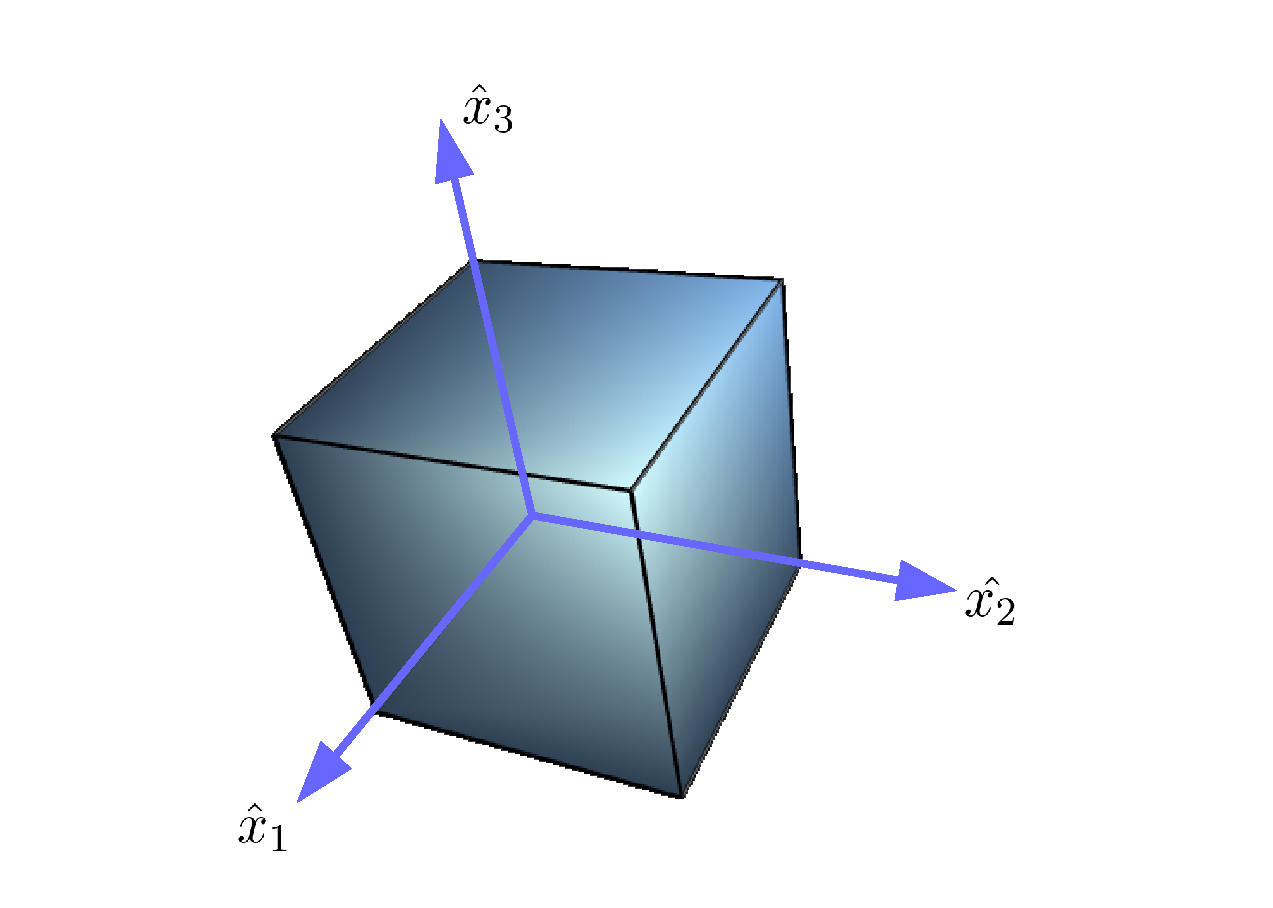
\includegraphics[scale=0.4]{images/c04-Orthogonality.eps}
 }
\end{center}
\caption{Orthogonal axes}
\label{orthogonalaxes1}
\end{figure}


Right-handed system: 
$$ \hat{x}_1 \cdot \left( \hat{x}_2 \times \hat{x}_3 \right) = 1 $$

$$ \hat{x}_1 \cdot \hat{x}_1 = \hat{x}_2 \cdot \hat{x}_2 = \hat{x}_3 \cdot \hat{x}_3 = 1 $$
$$ \hat{x}_1 \cdot \hat{x}_2 = \hat{x}_1 \cdot \hat{x}_3 = \hat{x}_2 \cdot \hat{x}_3 = 0 $$


If a coordinate system is rotated, how are the unit vectors of the two systems related?

\begin{figure}[h]
\begin{center}
\framebox{
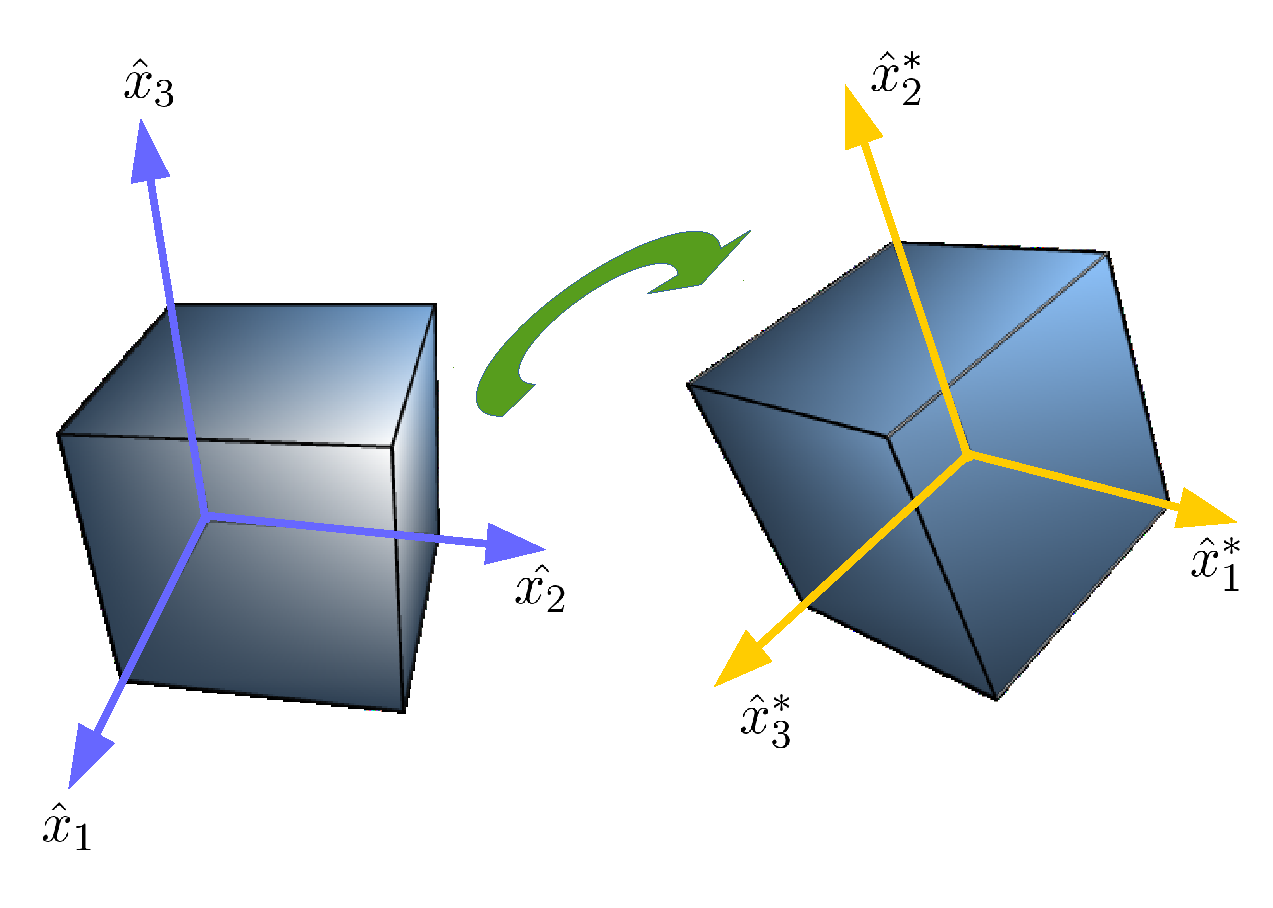
\includegraphics[scale=0.52]{images/c04-RotationIllustration.eps}
 }
\end{center}
\caption{Illustration of simple rotation of coordinate system}
\label{rotationofaxes}
\end{figure}



{\bf An example of coordinate transformation}

Consider rotating the coordinate system about $\hat{x}_3$ by an arbitrary angle $\theta$.

\begin{figure}[h]
\begin{center}
\framebox{
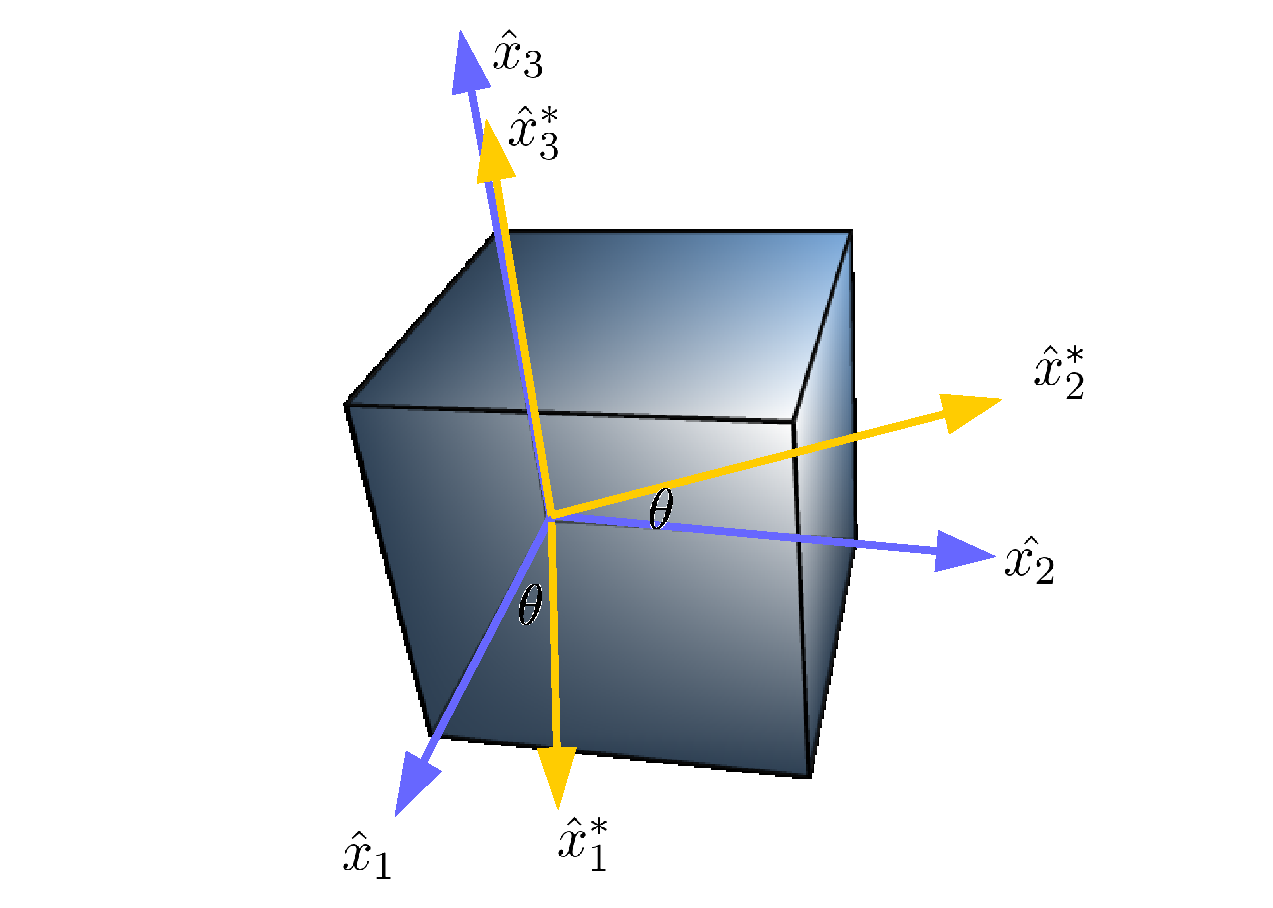
\includegraphics[scale=0.5]{images/c04-SimpleRotation.eps}
 }
\end{center}
\caption{Simple rotation about $\hat{x}_3$ axis}
\label{rotationofaxes2}
\end{figure}


{\bf New unit vectors in terms of old ones}

\begin{figure}[h]
\begin{center}
\framebox{
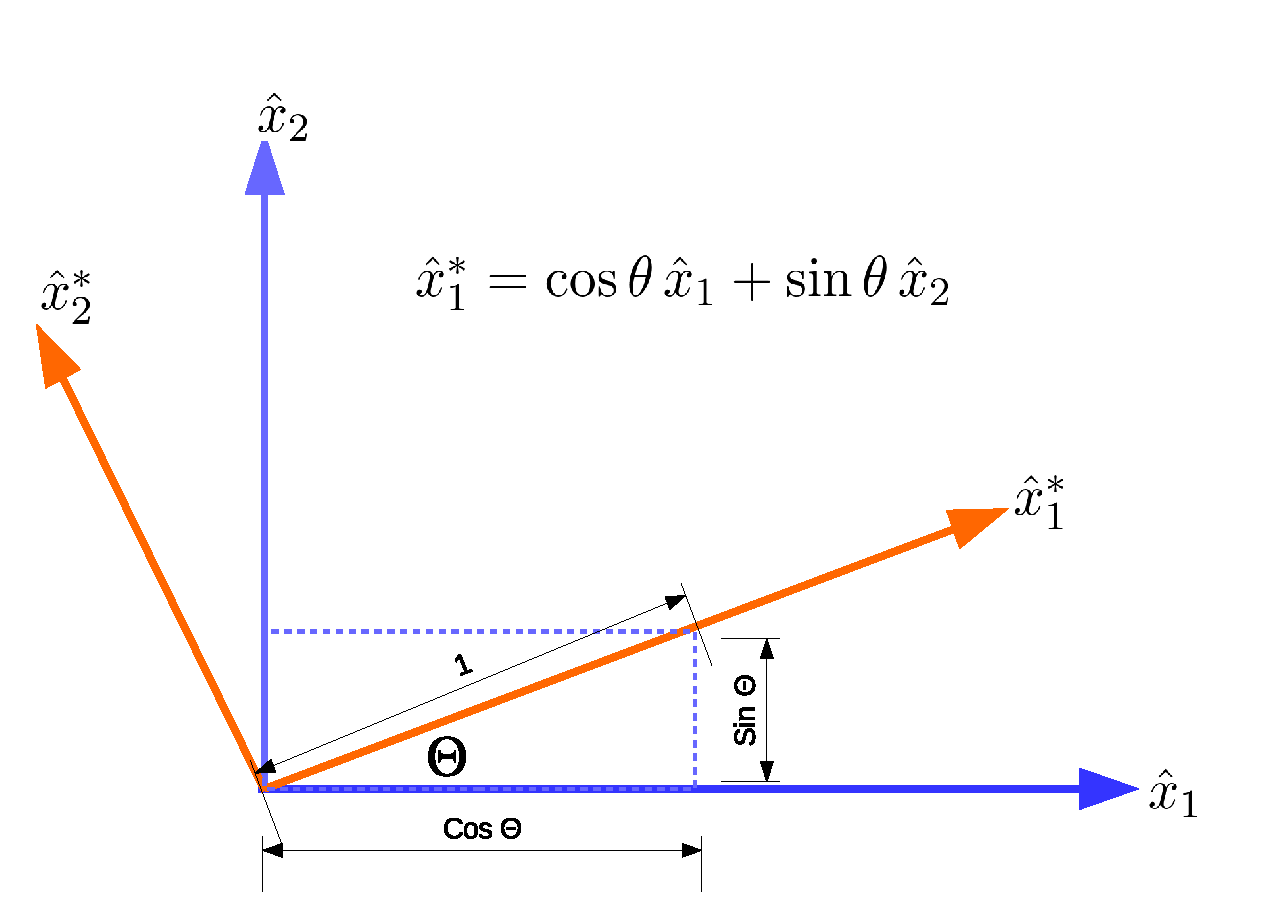
\includegraphics[scale=0.52]{images/c04-CoordinateRotations-1.eps}
 }
\end{center}
\caption{New unit vector $\hat{x}_1$ in terms of old ones after coordinate rotation}
\label{rotationofaxes3}
\end{figure}



\begin{figure}[h]
\begin{center}
\framebox{
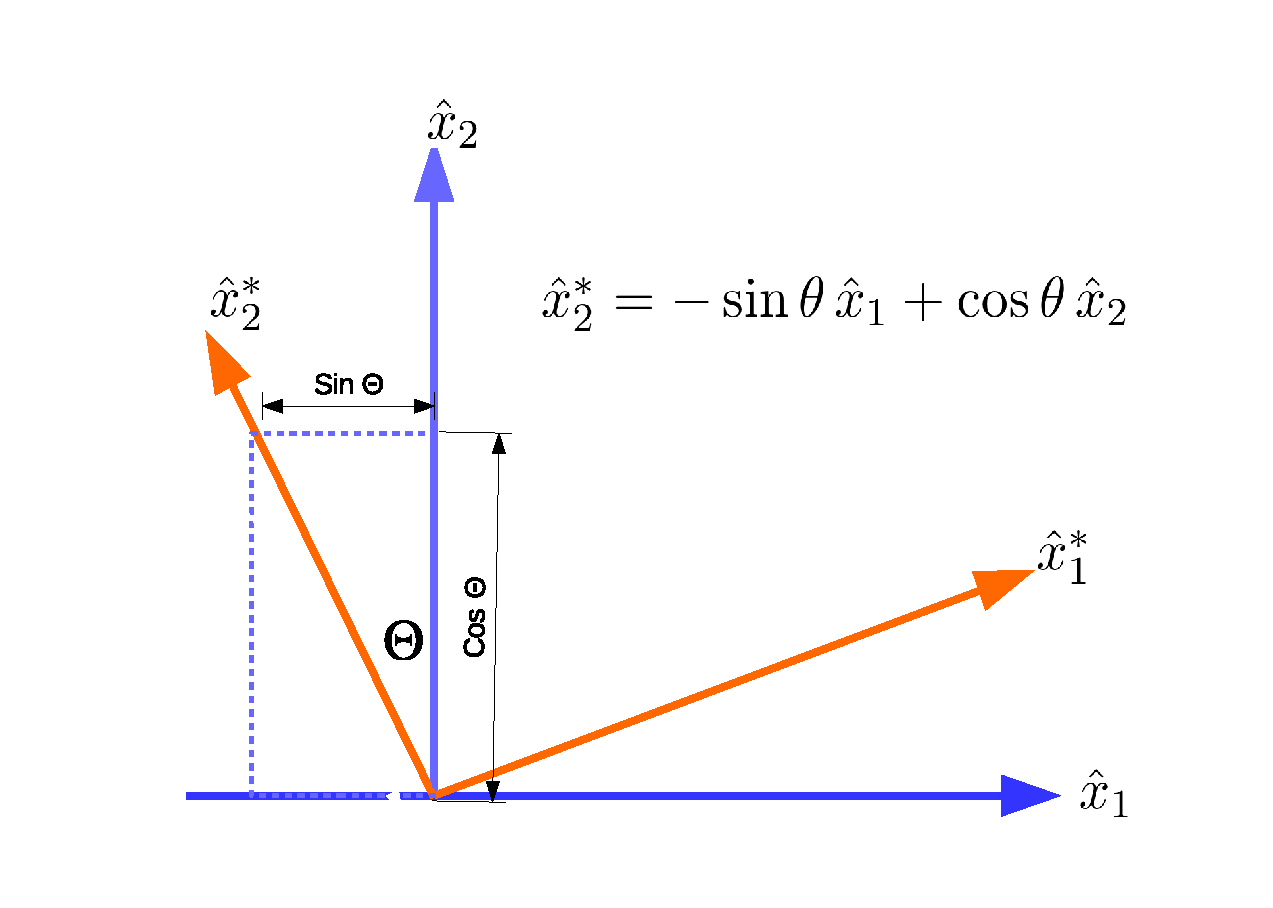
\includegraphics[scale=0.52]{images/c04-CoordinateRotations-2.eps}
 }
\end{center}
\caption{New unit vector $\hat{x}_2$ in terms of old ones after coordinate rotation}
\label{rotationofaxes4}
\end{figure}


$$ \hat{x}^*_1 = \cos\theta \, \hat{x}_1 + \sin\theta \, \hat{x}_2 + 0 \, \hat{x}_3 $$ 
$$ \hat{x}^*_2 = -\sin\theta \, \hat{x}_1 + \cos\theta \, \hat{x}_2 + 0 \, \hat{x}_3 $$ 
$$ \hat{x}^*_3 = 0 \, \hat{x}_1 + 0 \, \hat{x}_2 + \hat{x}_3 $$ 

or

\begin{equation*}
\left[ 
\begin{array}{l}
\hat{x}_1^*  \\
\hat{x}_2^* \\
\hat{x}_3^*  \\
\end{array}
\right] 
= \left[ 
\begin{array}{lll}
 \cos\theta  &  \sin\theta  & 0\\
 -\sin\theta &  \cos\theta  & 0 \\
  0 & 0 & 1\\
\end{array}
\right] 
\left[ 
\begin{array}{l}
\hat{x}_1 \\
\hat{x}_2 \\
\hat{x}_3 \\
\end{array}
\right]
\end{equation*}

\begin{equation*}
\left[ 
\begin{array}{l}
\hat{x}_1^*  \\
\hat{x}_2^* \\
\hat{x}_3^*  \\
\end{array}
\right] 
= \left[ 
\begin{array}{lll}
 T_{11}  &  T_{12}  & T_{13}\\
 T_{21}  &  T_{22}  & T_{23}\\
 T_{31}  &  T_{32}  & T_{33}\\
\end{array}
\right] 
\left[ 
\begin{array}{l}
\hat{x}_1 \\
\hat{x}_2 \\
\hat{x}_3 \\
\end{array}
\right]
\end{equation*}

Where
\begin{equation*}
T 
= \left[ 
\begin{array}{lll}
 \cos\theta  &  \sin\theta  & 0\\
 -\sin\theta &  \cos\theta  & 0 \\
  0 & 0 & 1\\
\end{array}
\right] 
\end{equation*}

Using subscript notation,

$$ \hat{x}^*_p = T_{pi} \hat{x}_i $$

{\bf Old unit vectors in terms of new ones}

\begin{figure}[h]
\begin{center}
\framebox{
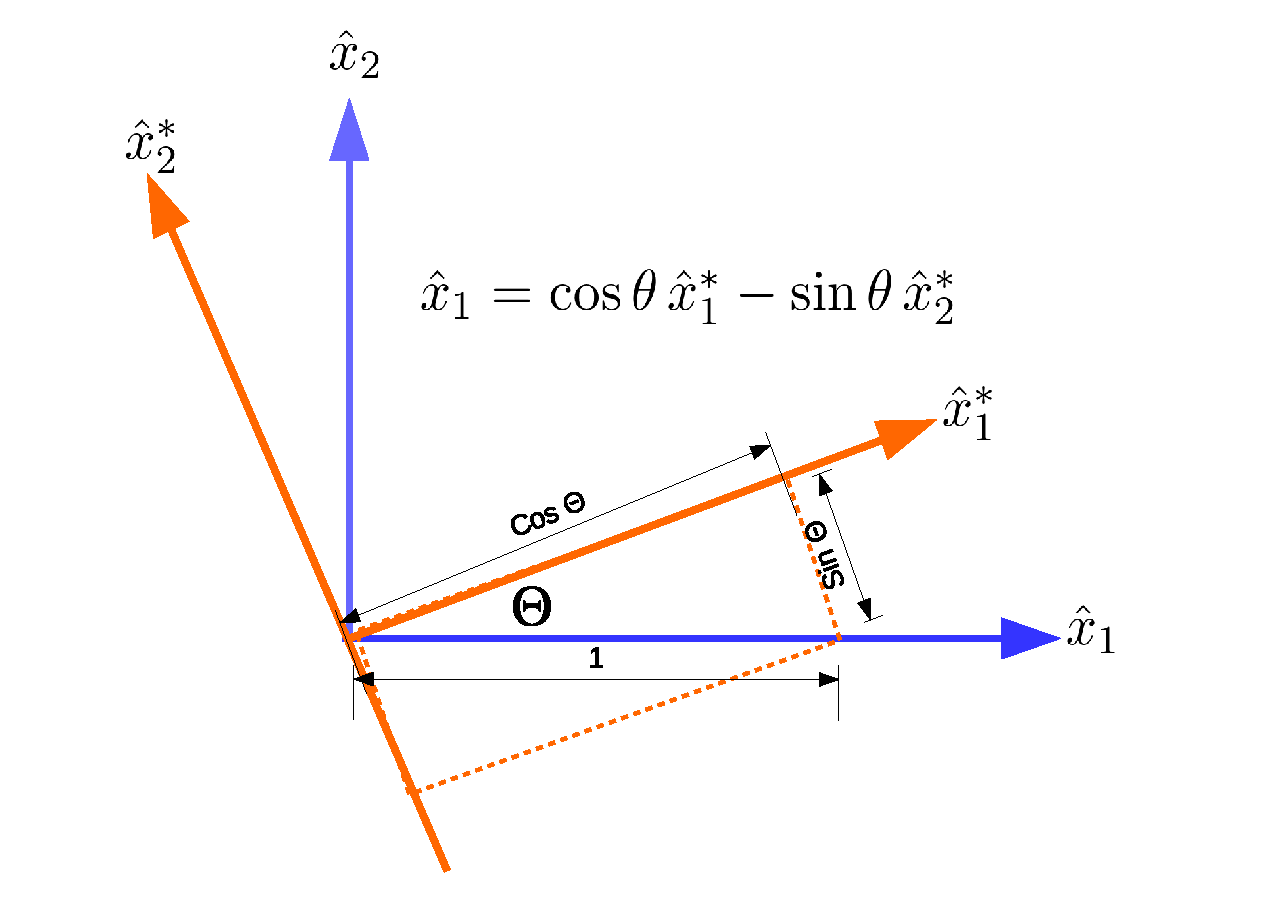
\includegraphics[scale=0.52]{images/c04-CoordinateRotations-3.eps}
 }
\end{center}
\caption{Old unit vector $\hat{x}_1$ in terms of new ones after coordinate rotation}
\label{rotationofaxes5}
\end{figure}



\begin{figure}[h]
\begin{center}
\framebox{
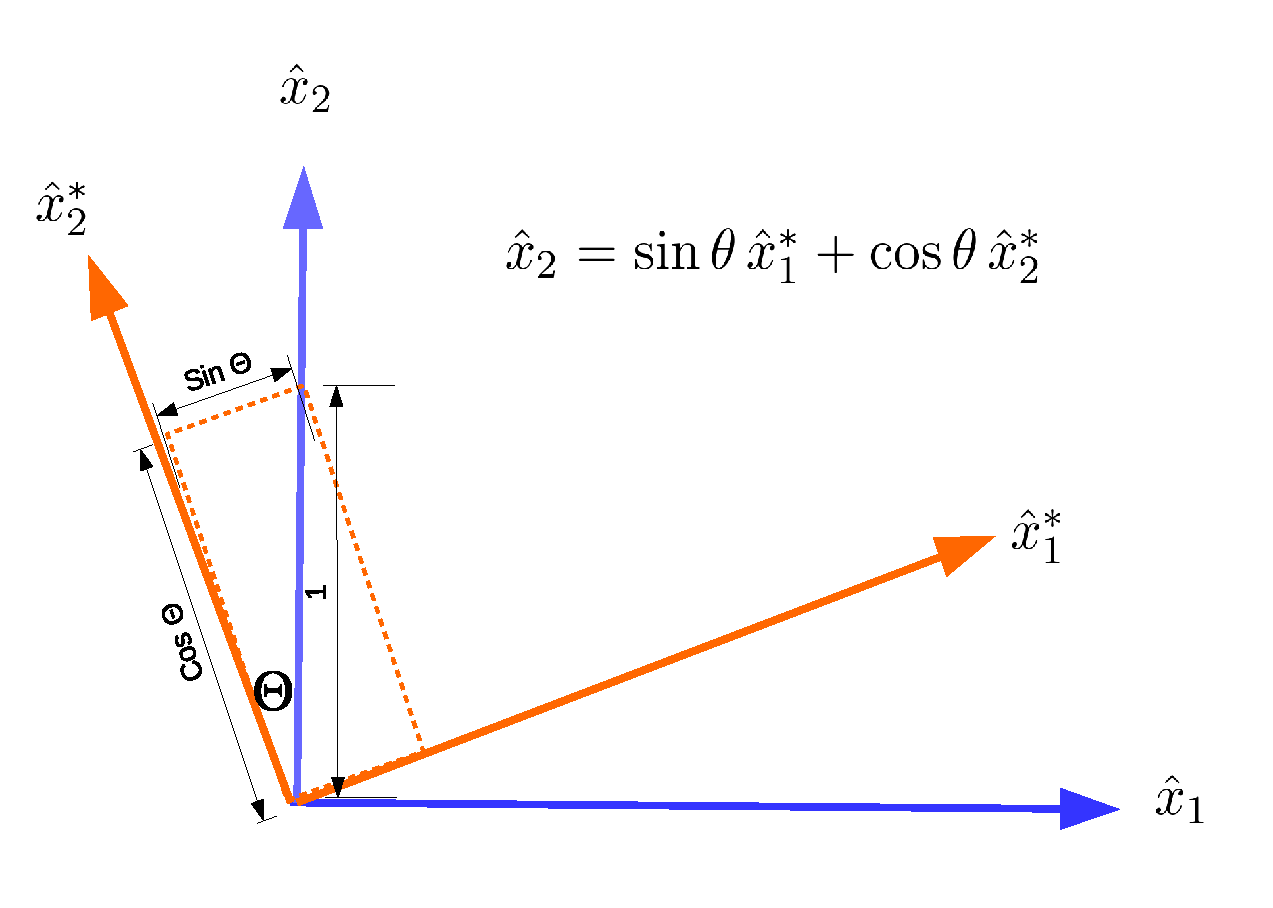
\includegraphics[scale=0.52]{images/c04-CoordinateRotations-4.eps}
 }
\end{center}
\caption{Old unit vector $\hat{x}_2$ in terms of new ones after coordinate rotation}
\label{rotationofaxes6}
\end{figure}



$$ \hat{x}_1 = \cos\theta \, \hat{x}^*_1 + -\sin\theta \, \hat{x}^*_2 + 0 \, \hat{x}^*_3 $$ 
$$ \hat{x}_2 = \sin\theta \, \hat{x}^*_1 + \cos\theta \, \hat{x}_2 + 0 \, \hat{x}_3 $$ 
$$ \hat{x}_3 = 0 \, \hat{x}^*_1 + 0 \, \hat{x}^*_2 + \hat{x}^*_3 $$ 

or

\begin{equation*}
\left[ 
\begin{array}{l}
\hat{x}_1  \\
\hat{x}_2 \\
\hat{x}_3  \\
\end{array}
\right] 
= \left[ 
\begin{array}{lll}
 \cos\theta  &  -\sin\theta  & 0\\
 \sin\theta &  \cos\theta  & 0 \\
  0 & 0 & 1\\
\end{array}
\right] 
\left[ 
\begin{array}{l}
\hat{x}^*_1 \\
\hat{x}^*_2 \\
\hat{x}^*_3 \\
\end{array}
\right]
\end{equation*}

Using subscript notation,

$$ \hat{x}_i = T_{pi} \hat{x}^*_p $$


{\bf Watch out the sequence of indices}

Transformation of old to new coordinate system:

$$ \hat{x}^*_p = T_{pi} \hat{x}_i $$
\begin{equation*}
\left[ 
\begin{array}{l}
\hat{x}_1^*  \\
\hat{x}_2^* \\
\hat{x}_3^*  \\
\end{array}
\right] 
= \left[ 
\begin{array}{lll}
T_{11} & T_{12} & T_{13} \\
T_{21} & T_{22} & T_{23} \\
T_{31} & T_{32} & T_{33} \\
\end{array}
\right] 
\left[ 
\begin{array}{l}
\hat{x}_1 \\
\hat{x}_2 \\
\hat{x}_3 \\
\end{array}
\right]
\end{equation*}

Transformation of new back to old coordinate system:

$$ \hat{x}_i = T_{pi} \hat{x}^*_p $$
\begin{equation*}
\left[ 
\begin{array}{l}
\hat{x}_1  \\
\hat{x}_2 \\
\hat{x}_3  \\
\end{array}
\right] 
= \left[ 
\begin{array}{lll}
T_{11} & T_{12} & T_{13} \\
T_{21} & T_{22} & T_{23} \\
T_{31} & T_{32} & T_{33} \\
\end{array}
\right] 
\left[ 
\begin{array}{l}
\hat{x}^*_1 \\
\hat{x}^*_2 \\
\hat{x}^*_3 \\
\end{array}
\right]
\end{equation*}


Watch out the sequence of indices !	

For old to new coordinate system, the convention is:

$$ \hat{x}^*_p = T_{pi} \hat{x}_i $$

Where, $p$ is the index for new- and $i$ is the index for old- coordinate systems.

{\bf Alternate definition of $T_{pi}$}

Consider the transformation from old to new coordinate system:
$$ \hat{x}^*_p = T_{pi} \hat{x}_i $$
Expand for $p=1$:
$$ \hat{x}^*_1 = T_{1i} \hat{x}_i = T_{11} \hat{x}_1 + T_{12} \hat{x}_2 + T_{13} \hat{x}_3 $$


This means one can also write the elements of $T_{pi}$ as

$$ T_{11} ={\partial \hat{x}^*_1 \over \partial \hat{x}_1 } $$
$$ T_{12} ={\partial \hat{x}^*_1 \over \partial \hat{x}_2 } $$
$$ T_{13} ={\partial \hat{x}^*_1 \over \partial \hat{x}_3 } $$

$$ T_{pi} = {\partial \hat{x}^*_p \over \partial \hat{x}_i} $$

% -----------------------------------------------------------------------


Consider the transformation from new to old coordinate system:
$$ \hat{x}_i = T_{pi} \hat{x}^*_p $$
Expand for $i=1$:
$$ \hat{x}_1 = T_{p1} \hat{x}^*_p = T_{11} \hat{x}^*_1 + T_{21} \hat{x}^*_2 + T_{31} \hat{x}^*_3 $$

Write the elements of $T_{pi}$ as
$$ T_{11} ={\partial \hat{x}_1 \over \partial \hat{x}^*_1 } $$
$$ T_{21} ={\partial \hat{x}_1 \over \partial \hat{x}^*_2 } $$
$$ T_{31} ={\partial \hat{x}_1 \over \partial \hat{x}^*_3 } $$

$$ T_{pi} = {\partial \hat{x}_i \over \partial \hat{x}^*_p} $$
$$ T_{pi} = {\partial \hat{x}^*_p \over \partial \hat{x}_i} = {\partial \hat{x}_i \over \partial \hat{x}^*_p}$$

{\bf Yet another definition of $T_{pi}$}

Consider the transformation from old to new coordinate system:
$$ \hat{x}^*_p = T_{pi} \hat{x}_i $$
Expand for $p=1$:
$$ \hat{x}^*_1 = T_{1i} \hat{x}_i = T_{11} \hat{x}_1 + T_{12} \hat{x}_2 + T_{13} \hat{x}_3 $$


This means one can also write the elements of $T_{pi}$ as

$$ \hat{x}^*_1 \cdot  \hat{x}_1 = T_{11} $$
$$ \hat{x}^*_1 \cdot \hat{x}_2 = T_{12} $$
$$ \hat{x}^*_1  \cdot \hat{x}_3 = T_{13} $$


$$ T_{pi} =  \hat{x}^*_p \cdot \hat{x}_i $$


% -----------------------------------------------------------------------

{\bf Properties of $T_{pi}$ using orthogonality}

$$ \hat{x}^*_1 \cdot \hat{x}^*_1 = 1 $$
$$ \hat{x}^*_1 = T_{1i} \hat{x}_i $$
$$ T_{1i} T_{1i} = 1 = \delta_{11} $$

$$ \hat{x}^*_1 \cdot \hat{x}^*_2 = 0 $$
$$ \hat{x}^*_1 = T_{1i} \hat{x}_i $$
$$ \hat{x}^*_2 = T_{2i} \hat{x}_i $$
$$ T_{1i} T_{2i} = 0 = \delta_{12} $$

$$ \hat{x}^*_1 \cdot \hat{x}^*_3 = 0 $$
$$ \hat{x}^*_1 = T_{1i} \hat{x}_i $$
$$ \hat{x}^*_3 = T_{3i} \hat{x}_i $$
$$ T_{1i} T_{3i} = 0 = \delta_{13} $$

Generalizing,

$$ T_{mi} T_{ni} = \delta_{mn} $$

Similarly, using the orthogonality of the old coordinate system, we can get

$$ T_{im} T_{in} = \delta_{mn} $$


% -----------------------------------------------------------------------

{\bf Properties of transformation matrix}

\begin{itemize}
\item $T_{pi}$ is determined by the rotation of the coordinate system
\item Determinant of $T_{pi}$ is 1
\item Inverse of $T_{pi}$ is its transpose, namely $T_{ip}$
\item Orthogonality leads to $ T_{mi} T_{ni} = \delta_{mn} $ and $ T_{im} T_{in} = \delta_{mn} $
\end{itemize}


% -----------------------------------------------------------------------

{\bf Components of a vector across coordinate rotation}

\begin{figure}[h]
\begin{center}
\framebox{
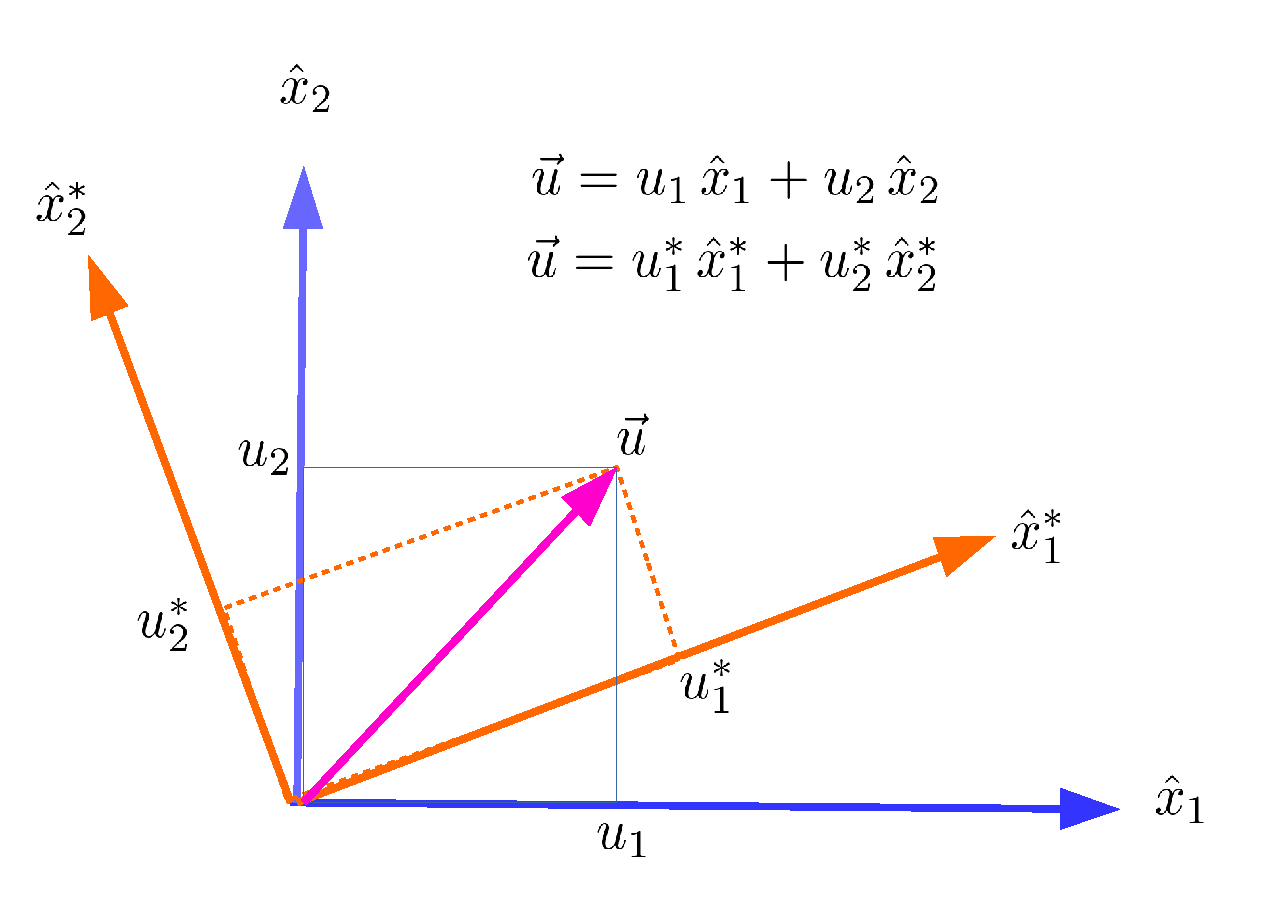
\includegraphics[scale=0.52]{images/c04-CoordinateRotations-5.eps}
 }
\end{center}
\caption{Components of a vector across coordinate rotation}
\label{rotationofaxes7}
\end{figure}


% -----------------------------------------------------------------------

{\bf Components of a vector across coordinate rotation}

$$ \vec{u} = u_1 x_1 + u_2 x_2 + u_3 x_3 $$
$$ = u_1 \left( \cos\theta \, \hat{x}^*_1 + \sin\theta \, \hat{x}^*_2 + 0 \, \hat{x}^*_3 \right) + $$
$$ + u_2 \left( -\sin\theta \, \hat{x}^*_1 + \cos\theta \, \hat{x}^*_2 + 0 \, \hat{x}^*_3 \right) +$$
$$ + u_3 \left( 0 \, \hat{x}^*_1 + 0 \, \hat{x}^*_2 + \hat{x}^*_3 \right) $$

$$ = \left( u_1 \cos\theta + u_2 \sin\theta \right) \hat{x}^*_2 + \left( -u_1 \sin\theta + u_2 \cos\theta \right) \hat{x}^*_2 + u_3 \hat{x}^*_3 $$

$$ = u^*_1 x^*_1 + u^*_2 x^*_2 + u^*_3 x^*_3  $$


% -----------------------------------------------------------------------

{\bf Components of a vector across coordinate rotation}

\begin{equation*}
\left[ 
\begin{array}{l}
u^*_1  \\
u^*_2 \\
u^*_3  \\
\end{array}
\right] 
= \left[ 
\begin{array}{lll}
 \cos\theta  &  \sin\theta  & 0\\
 -\sin\theta &  \cos\theta  & 0 \\
  0 & 0 & 1\\
\end{array}
\right] 
\left[ 
\begin{array}{l}
u_1 \\
u_2 \\
u_3 \\
\end{array}
\right]
\end{equation*}

or

$$ u^*_p = T_{pi} u_i $$

This equation preserves the nature of $\vec{u}$ across coordinate transforms and is thus a way to {\bf define} a vector.


% -----------------------------------------------------------------------

{\bf Definition of a vector}

A bunch of three numbers $u_i$ that follow the following relation across a coordinate transformation are components of a vector $\vec{u}$

{\bf Definition}
$$ u^*_p = T_{pi} u_i $$

A vector field is a vector that is a function of a location. 

{\bf Examples}
Velocity field $u\left(x,y,z\right)$, Gradient of thermal field $\vec{\nabla}T\left(r,\theta,z\right)$, Gradient of composition $\vec{\nabla}C_A\left(x,y,z\right)$, Electric field $E\left(x,y,z,\right)$ etc.,


% -----------------------------------------------------------------------

{\bf Definition of a scalar}

Scalar is a quantity which is invariant (does not change) across a coordinate transformation.

{\bf Examples}
Temperature $T$, Energy $G$, density $\rho$ etc.,

A scalar field is a scalar that is a function of location. 

{\bf Examples}
Thermal field $T\left(x,y,z\right)$, Density field $\rho\left(r,\theta,z\right)$, Phase field $\phi\left(x,y,z,\right)$ etc.,

Value of a scalar field at a location should not change if the coordinates chosen to represent the location change.


% ----------------------------------------------------------------------------------------

Cartesian co-ordinate system $\hat{x}_i$ is used. Consider the following co-ordinate transformation where the xy plane is rotated about z-axis clockwise by an angle $\theta$. 
\vspace{1cm}

%\begin{figure}[h]
% \centering
% \includegraphics[width=5 in]{images/ctrans0.eps}
% % ctrans.eps: 46x0 pixel, 300dpi, 0.39x0.00 cm, bb=0 35 595 420
% \caption{Co-ordinate Transformation}
% \label{ctrans}
%\end{figure}


The new axes (starred) are given in terms of the old axes (unstarred) by the following relations:

\begin{equation}
\begin{array}{l}
\hat{x}_1^* =  \hat{x}_1 cos\theta + \hat{x}_2 sin\theta \\
\hat{x}_2^* =  -\hat{x}_1 sin\theta + \hat{x}_2 cos\theta \\
\hat{x}_3^* =  \hat{x}_3 \\
\end{array}
\end{equation}
or
\begin{equation}
\label{oldnew}
\begin{array}{l}
\hat{x}_1^* = T_{11}\hat{x}_1 + T_{12}\hat{x}_2 + T_{13}\hat{x}_3\\
\hat{x}_2^* = T_{21}\hat{x}_1 + T_{22}\hat{x}_2 + T_{23}\hat{x}_3\\
\hat{x}_3^* = T_{31}\hat{x}_1 + T_{32}\hat{x}_2 + T_{33}\hat{x}_3\\
\end{array}
\end{equation}

\begin{equation}
\left( 
\begin{array}{l}
\hat{x}_1^*  \\
\hat{x}_2^* \\
\hat{x}_3^*  \\
\end{array}
\right) 
= \left( 
\begin{array}{lll}
 cos\theta  &  sin\theta  & 0\\
 -sin\theta &  cos\theta  & 0 \\
  0 & 0 & 1\\
\end{array}
\right) 
\left( 
\begin{array}{l}
\hat{x}_1 \\
\hat{x}_2 \\
\hat{x}_3 \\
\end{array}
\right)
\end{equation}

or

\begin{equation}
\label{vecdeff}
\boxed{
\hat{x}_p^* = T_{pi}\hat{x}_i
}
\end{equation} 

The transformation matrix \index{Transformation matrix} $T_{pi}$ used in the above expression is by the convention that first index represents the row and the second index, the column. In one of the reference texts, viz., Aris' book ~\cite{aris}, equation (2.11.1) shows that this convention is reversed. As a result the indices appear swapped in the definitions. This use of different convention is clear also from equation (A.6.4) in the same book.

When we express $x_i^*$ in terms of $x_i$, the {\bf transformation matrix} can be written as: 

\begin{equation}
T_{pi} = \frac{\partial \hat{x}_p^*}{\partial \hat{x}_i} =
\left( 
\begin{array}{lll}
\frac{\partial \hat{x}_1^*}{\partial \hat{x}_1} &
\frac{\partial \hat{x}_1^*}{\partial \hat{x}_2} &
\frac{\partial \hat{x}_1^*}{\partial \hat{x}_3} \\
\\
\frac{\partial \hat{x}_2^*}{\partial \hat{x}_1} &
\frac{\partial \hat{x}_2^*}{\partial \hat{x}_2} &
\frac{\partial \hat{x}_2^*}{\partial \hat{x}_3} \\
\\
\frac{\partial \hat{x}_3^*}{\partial \hat{x}_1} &
\frac{\partial \hat{x}_3^*}{\partial \hat{x}_2} &
\frac{\partial \hat{x}_3^*}{\partial \hat{x}_3} \\
\end{array}
\right) 
\end{equation}

We have chosen cartesian co-ordinate systems which have the following properties of {\em orthogonality} \index{Orthogonality}:

\begin{equation}
\label{ortho}
\begin{array}{lll}
\hat{x}^*_1 \cdot \hat{x}^*_1 = 1 & \hat{x}^*_2 \cdot \hat{x}^*_3 = 0 & \hat{x}^*_3 \cdot \hat{x}^*_2 = 0  \\
\hat{x}^*_2 \cdot \hat{x}^*_2 = 1 & \hat{x}^*_3 \cdot \hat{x}^*_1 = 0 & \hat{x}^*_1 \cdot \hat{x}^*_3 = 0  \\
\hat{x}^*_3 \cdot \hat{x}^*_3 = 1 & \hat{x}^*_1 \cdot \hat{x}^*_2 = 0 & \hat{x}^*_3 \cdot \hat{x}^*_1 = 0 \\
\end{array} 
\end{equation} 


Expressing $\hat{x}^*$ in terms of $\hat{x}$ and using equations~\ref{oldnew} and \ref{ortho}, we get:

\begin{equation}
\begin{array}{l}
T_{11}T_{12} + T_{21}T_{22} + T_{31}T_{32} = 0 \\
T_{12}T_{13} + T_{22}T_{23} + T_{32}T_{33} = 0 \\
T_{13}T_{11} + T_{23}T_{21} + T_{33}T_{31} = 0 \\
T_{11}T_{11} + T_{12}T_{12} + T_{13}T_{13} = 1 \\
T_{21}T_{21} + T_{22}T_{22} + T_{23}T_{23} = 1 \\
T_{31}T_{31} + T_{32}T_{32} + T_{33}T_{33} = 1
\end{array} 
\end{equation} 

or 

\begin{equation}
\boxed{
T_{ij}T_{ik} = \delta_{jk} 
}
\end{equation} 

{\bf Rotating the co-ordinate system back...}

Similarly, we can express $\hat{x}$ in terms of $\hat{x}^*$. Inverse transformation relation is given using the transpose of the transformation matrix as follows. Transpose of a matrix is nothing but the same matrix with the indices swapped around.
$$ \hat{x}_i = D_{ip} \hat{x}_p^*$$

The co-ordinate transformation matrix $D$ for new to old system is related to the matrix for old to new the following manner.

$$ D_{ip} = T_{ip}^{-1}= T_{ip}^{T} = T_{pi} $$

$$ \hat{x}_i = D_{ip} \hat{x}_p^* = T_{pi} \hat{x}_p^*$$

\begin{equation}
\label{vecdefr}
\boxed{\hat{x}_i = T_{pi} \hat{x}_p^*}
\end{equation}

{\bf Note:} Compare equations \ref{vecdeff} and \ref{vecdefr} and notice which of the indices is being repeated in the RHS.

Exploiting the orthogonality of the old co-ordinate system:

\begin{equation}
\begin{array}{lll}
\hat{x}_1 \cdot \hat{x}_1 = 1 & \hat{x}_2 \cdot \hat{x}_3 = 0 & \hat{x}_3 \cdot \hat{x}_2 = 0 \\
\hat{x}_2 \cdot \hat{x}_2 = 1 & \hat{x}_3 \cdot \hat{x}_1 = 0 & \hat{x}_1 \cdot \hat{x}_3 = 0 \\
\hat{x}_3 \cdot \hat{x}_3 = 1 & \hat{x}_1 \cdot \hat{x}_2 = 0 & \hat{x}_2 \cdot \hat{x}_3 = 0 \\
\end{array} 
\end{equation} 


\begin{equation}
\boxed{
T_{ji}T_{ki} = \delta_{jk}
}
\end{equation} 


\section{Scaffold to determine transformation matrix}

\begin{mdframed}[style=tpscaffold1]
\begin{enumerate}

\item For a rotation of a coordinate system about $\hat{x}_3$ by 90 degrees, anti-clockwise, express the unit vectors of the new coordinate system in terms of those of the old coordinate system. Write down how the transformation matrix would look like.

\item For a rotation of a coordinate system about $\hat{x}_3$ by 90 degrees, clockwise, write down how the transformation matrix would look like.

\item Write the unit vectors of the new coordinate system $\hat{x}_i^*$ in terms of $T_{ij}$ and unit vectors of the old coordinate system $\hat{x}_i$. Use the orthogonality properties of the unit vectors in the new coordinate system and determine what values the expression $T_{ij}T_{ik}$ would take.

\item If the transformation matrix for coordinate system rotation from $\hat{x}_i$ (old) to $\hat{x}_p^*$ (new) is $T_{pi}$ then convince yourself that the transformation matrix for rotating the new coordinate system back to the old one is the transpose of $T_{pi}$.

\item Write the unit vectors of the old coordinate system $\hat{x}_i$ in terms of $T_{ij}$ and unit vectors of the new coordinate system $\hat{x}_p^*$. Use the orthogonality properties of the unit vectors in the new coordinate system and determine what values the expression such as $T_{ji}T_{ki}$ would take.

\item Based on the answers to the above questions, generalize a rule when two terms of type $T_{ij}$ were to come together in an expression that involves summation over any index.

\end{enumerate}
\end{mdframed}

\section{Rodrigues rotation formula}

% learning objective
\begin{lo3}[Coordinate transforms]
Determine components of a transformation matrix given the axis and angle of rotation of a rectangular coordinate system
\end{lo3}


The transformation matrix for rotation of a coordinate system about an arbitrary axis given by the unit vector $\hat{n}$ by an arbitrary angle $\theta$ is given by:

\begin{equation}
R_{ij} = \cos\theta \, \delta_{ij} + \left( 1 - \cos \theta \right) \, n_i \, n_j - \sin\theta \epsilon_{ijk} n_k
\end{equation}

\begin{equation}
\hat{n} = n_i \hat{i} + n_j \hat{j} + n_k \hat{k}
\end{equation}

\begin{equation}
n_i^2 + n_j^2 + n_k^2 = 1
\end{equation}

The transformation matrix when expanded looks like the following.

\begin{align*}
\end{align*}

\begin{equation}
R_{ij}
= \left[ 
\begin{array}{lll}
\cos\theta + n_1^2\left( 1 - \cos\theta\right) & n_1 n_2 \left(1 - \cos\theta\right)-n_3 \sin\theta & n_1 n_3\left(1 - \cos\theta\right) + n_2 \sin\theta \\
n_1 n_2 \left( 1 - \cos\theta \right) + n_3 \sin\theta  &  \cos\theta + n_2^2 \left(1 - \cos\theta\right) & n_2 n_3\left(1 - \cos\theta\right) - n_1 \sin\theta \\
n_1 n_3 \left( 1 - \cos\theta \right) - n_2 \sin\theta & n_2 n_3 \left(1 - \cos\theta\right) + n_1 \sin\theta & \cos\theta + n_3^2 \left(1 - \cos\theta\right)  \\
\end{array}
\right] 
\end{equation}

One can substitute the values of $n_i$ for the unit vector $\hat{n}$ about which a rotation is being made, along with the value for $\theta$ for the angle of rotation and obtain the components of the transformation matrix $R_{ij}$ readily.

% ----------------------------------------------------------------------------

\begin{question}
	Show that the following matrix is a possible transformation matrix for coordinate rotation about a fixed point. 
\begin{equation}
T_{ij}
= \left[ 
\begin{array}{lll}
	\sin\theta \cos\phi & \sin\theta \sin\phi & \cos\theta \\
	\cos\theta \cos\phi & \cos\theta \sin\phi & -\sin\theta \\
	-\sin\phi & \cos\phi & 0
\end{array}
\right] 
\end{equation}

\end{question}
\begin{solution}[print]
	Show that the determinant is unity and that the orthogonality relations apply.
\end{solution}

% ----------------------------------------------------------------------------

\begin{question}
	If $T_{ij}$ is a transformation matrix, show that the following relations apply.
	$$ T_{11} = T_{22} T_{33} - T_{23} T_{32} $$
	$$ T_{12} = T_{23} T_{31} - T_{21} T_{33} $$
	$$ T_{13} = T_{21} T_{32} - T_{22} T_{31} $$

\end{question}
\begin{solution}[print]
	Consider the terms in $T_{ij}$ as direction cosines and compare the terms using the expression for determinant $\text{Det}\left(T_{ij}\right)=1$
\end{solution}

% ----------------------------------------------------------------

\section{Summary}

\begin{enumerate}
\item Orthogonality relations can be used to simplify terms while determining isotropy of a tensor
\end{enumerate}

% ----------------------------------------------------------------

\chapter{Introduction to Cartesian Tensors}
\label{ch:tensintro}

\section{Cartesian Tensors}

% learning objective
\begin{lo1}[Tensor introduction]
Recall the definitions of tensors and their order.
\end{lo1}


Many entities, such as those that have a physical meaning, are independent of the co-ordinate system we choose to represent them.  If $n$ is the dimension of the space we are concerned, the entities can be classifed - according to the number of components $(n^i)$ they would have - as {\bf tensors} of order $i$. 

\fbox{ %begin minipage frame
\begin{minipage}{4 in}
In this notes, when we say tensor, we imply Cartesian tensor. We don't want to get into covariant, contravariant and such things at this stage.
\end{minipage}
} % end of minipage frame



\subsection{Scalar}
Scalar is a tensor of order zero. Only one value would suffice to describe it at any location. Scalars are invariant under co-ordinate transformations.

{\bf Definition:} Scalar is an entity that remains invariant under all co-ordinate transformations.

Eg: Temperature $T$, Composition of - say - $A$ species $C_A$, Pressure in a fluid $p$, Density $\rho$, etc., 

\subsection{Vector}
Vector is a tensor of order one. It requires as many values / components as the dimension of the space (which is three for most of us) ie., a set of three components in a 3D space. 

{\bf Definition:} Vector is an entity that transforms the following way under a co-ordinate transformation: 
\begin{equation}
a^*_p = T_{pi}a_i
\end{equation} 

Eg: Velocity of fluid $\vec{u} = u_i$, Temperature gradient $\partial T \over \partial x_i$, Composition gradient $\partial C_A \over \partial x_i$, Displacement $u_i$, Electric Potential difference $P$, Electric Current $J_i$ etc.,

\subsection{Bisor}
Bisor is a tensor of order two. All tensors of order 2 or more are called as just {\bf tensors}. Specific names for tensors of order 2 and above are often considered old fashioned. A tensor of order 2 requires 9 components to describe it in general in 3D. 

{\bf Definition:} Tensor of order two is an entity that transforms the following way under a co-ordinate transformation: 
\begin{equation}
a^*_{pq} = T_{pi}T_{qj}a_{ij}
\end{equation} 

Eg: Stress $\sigma_{ij}$, Strain $e_{ij}$, Electrical Conductivity $\sigma_{ij}$, Electrical Resistivity $\rho_{ij}$, Diffusivity $D_{ij}$, Thermal Conductivity $k_{ij}$, Magnetic Permeability $\mu_{ij}$, Dielectric Permittivity $\epsilon_{ij}$, Thermal Expansion Coefficient $\alpha_{ij}$, Gyration Tensor $g_{ij}$

\subsection{Trisor}

Trisor is a tensor of order three. 27 components! 

{\bf Definition:} Tensor of order three is an entity that transforms the following way under a co-ordinate transformation: 
\begin{equation}
a^*_{pqr} = T_{pi}T_{qj}T_{rk}a_{ijk}
\end{equation} 

Eg: Piezoelectric coefficient $e_{ijk}$, 

\subsection{Tetror}

Tetror is a tensor of order four. 81 components! 
\begin{equation}
a^*_{pqrs} = T_{pi}T_{qj}T_{rk}T_{sl} a_{ijkl}
\end{equation}

Eg: Elastic Modulus $c_{ijkl}$

\subsection{Tensor}

\index{Tensor}

In general, a tensor is an entity that follows the following generalised rule for any co-ordinate transformation. The number of indices of $a$ indicate the order of the tensor which is the same as the number of times $T$ occurs in the expression.

\begin{equation}
\boxed{a^*_{pqrst...} = T_{pi}T_{qj}T_{rk}T_{sl}T_{tm}... a_{ijklm...} }
\end{equation}

% learning objective
\begin{lo2}[Tensor Introduction]
Validate a tensorial expression and identify the tensorial order of a parameter
\end{lo2}

Here we must bring in some examples.


\section{Operations on tensors}

\index{Tensor operations}

\begin{itemize}

\item Sum and difference of two tensors (of same order) is also a tensor. In the following example, if $b_{ij}$ and $c_{ij}$ are tensors, then $a_{ij}$ and $d_{ij}$ are also tensors.
$$ a_{ij} = b_{ij} + c_{ij} $$
$$ d_{ij} = b_{ij} - c_{ij} $$

\index{Dyadic product}
\item An outer product of a tensor of order $m$  with a tensor of order $n$ will give a tensor of order $m+n$. Outer product is also referred to as dyadic product.
$$a_{ijk} = b_{ij}c_{k}$$

\item An inner product of a tensor of order $m$ with a tensor of order $n$ will give a tensor of order $|m-n|$.
$$a_{i} = b_{ijk}c_{jk}$$

\index{Contraction theorem}
\item {\bf Contraction theorem}\label{contraction} \index{Contraction theorem} : If $a_{ijkl..}$ is a tensor of order $m$, then the entity obtained by repeating any two subscripts is a tensor of order $m-2$. Eg., if $d_{ijkl}$ is a tensor of order 4, then by repeating two of its indices (say, third and fourth), the entity obtained $a_{ij}$ is a tensor of order $4-2=2$.
$$ a_{ij} = d_{ijkk}$$


A corollary to the above theorem is obtained when we take a tensor of order two and repeat the indices. i.e., Trace of a second order tensor $a_{ii}$ is tensor of order zero or scalar or invariant across co-ordinate transformations.


\item {\bf Quotient law of tensors} \index{Quotient law}: If there is an entity representable by (subscript notation as) $a_{ij}$ relative to any cartesian co-ordinate system and if $a_{ij}b_i$ is a {\em vector} where $b_i$ is {\em any arbitrary vector} then $a_{ij}$ is a {\em tensor} of order two. Proof is given in section \ref{quotientrule}.

Combining with the theorem on outer product, quotient law can be extended to tensors of higher order.


\end{itemize}


\section{Types of tensors}

\subsection{Symmetric Tensor}
\index{Tensor, symmetric}

$a$ is a {\em symmetric} tensor if $a_{ij} = a_{ji}$

{\bf Theorem}: For every second order symmetric tensor, there exists a co-ordinate system relative to which, the matrix of the components of the tensor is diagonal \footnote{This theorem has important implications when applied to the stress tensor in the mechanical behaviour of materials. The diagonal terms are called principal stresses.}. Proof is given in section \ref{diagonalisable}.

\subsection{Anti-symmetric Tensor}
\index{Tensor, anti-symmetric}

$a$ is a {\em skew-symmetric} or {\em anti-symmetric} tensor if $a_{ij} = -a_{ji}$

The vector formed by the components of an anti-symmetric tensor:

$$
\omega_k = \left( 
\begin{array}{l}
\omega_1\\
\omega_2 \\ 
\omega_3
\end{array} 
\right)
$$

$$ \Omega_{ij} =  \left(
\begin{array}{ccc}
0 & \omega_3 & -\omega_2 \\
-\omega_3 & 0 & \omega_1 \\
\omega_2 & -\omega_1 & 0
\end{array} 
\right)
$$

$$\omega_k = \frac{1}{2} \epsilon_{kij} \Omega_{ij} $$
Also,
$$\Omega_{ij} = \epsilon_{ijk}\omega_{k}$$

\index{Dual tensors}
The two tensors $\omega_k$ and $\Omega_{ij}$ are called dual tensors.

{\bf Theorem}: Every second order tensor is expressible as a sum of a symmetric tensor and an anti-symmetric tensor. 

\begin{equation}
a_{ij} = \frac{1}{2}\left( a_{ij}+a_{ji}\right) + \frac{1}{2}\left( a_{ij}-a_{ji}\right) 
\end{equation} 



% ---------------------------------------------------------------------

% learning objective
\begin{lo2}[Tensor introduction]
Prove an expression to be a tensor of appropriate order using the definition of a tensor
\end{lo2}

% ---------------------------------------------------------------------

\begin{question}
Prove that gradient of a continuous scalar function is a vector. 
\begin{equation}
a_i = \nabla_i\phi = \frac{\partial \phi}{\partial x_i}
\end{equation} 
\end{question}
\begin{solution}[print]
\end{solution}

% ---------------------------------------------------------------------

\begin{question}
Prove that the magnitude of a vector is invariant under co-ordinate transformations.
\end{question}
\begin{solution}[print]
\end{solution}

% ---------------------------------------------------------------------

\begin{question}
Prove that $\delta_{ij}$ is (an isotropic) tensor of order two.
\end{question}
\begin{solution}[print]
\end{solution}

% ---------------------------------------------------------------------

\begin{question}
Prove that if $u_i$ and $v_j$ are vectors, then the dyad $a_{ij} = u_i v_j$ is a tensor of order two.
\end{question}
\begin{solution}[print]
\end{solution}

% ---------------------------------------------------------------------

\begin{question}
(Exercise 2.42.1 of \cite{aris}) Prove that for any vector $\vec{a}$, $\epsilon_{ijk}a_k$ are the components of a second order tensor.
\end{question}
\begin{solution}[print]
\end{solution}

% ---------------------------------------------------------------------

\begin{question}
(Exercise 2.42.3 and 2.44.2 of \cite{aris}) If $r^2 = x_k x_k$ and $f(r)$ is any twice differentiable function, show that the following nine derivatives are components of a tensor.
$$\left[ f''(r) -{f'(r) \over r} \right] {x_i x_j \over r^2} + {f'(r) \over r} \delta_{ij} $$.
Show also that the trace of that tensor is the following.
$${1 \over r^2}{d \over dr} \left( r^2 {df \over dr} \right)$$
\end{question}
\begin{solution}[print]
\end{solution}

% ---------------------------------------------------------------------

\begin{question}
Prove that strain rate or velocity gradient is a tensor of order two.
$$ e_{ij} = {\partial u_i \over \partial x_j}$$
\end{question}
\begin{solution}[print]
\end{solution}

% ---------------------------------------------------------------------

\begin{question}
If $\sigma_{ij}$ is a tensor, prove that $\sigma_{ii}$, the trace of the matrix of $\sigma_{ij}$ is invariant under co-ordinate transformations. \footnote{This quantity has a special meaning in mechanical behaviour of materials.}
\end{question}
\begin{solution}[print]
\end{solution}

% ---------------------------------------------------------------------

\begin{question}
Prove that $\epsilon_{ijk}$ is a tensor of order three. Clue: Use the subscript notation for determinant of the transformation matrix. When two rows of a matrix are same, the determinant vanishes.
\end{question}
\begin{solution}[print]
\end{solution}

% ---------------------------------------------------------------------

\begin{question}
Prove that the dyad $\delta_{ij}\delta_{kl}$ is (an isotropic) tensor of order four. Considering that $\delta_{ij}$ is an isotropic and hence a symmetric tensors, how many combinations of the four indices can you get so that you can arrive at possible isotropic tensors of order four.
\end{question}
\begin{solution}[print]
\end{solution}

% ---------------------------------------------------------------------

\begin{question}
If $a_{ij}$ and $b_{kl}$ are tensors of order two, prove that the dyad $a_{ij} b_{kl}$ is a tensor of order four. Prove that $a_{ij} b_{jk}$ is a tensor of order two. Also, that $a:b = a_{ij}b_{ji}$ is a scalar.
\end{question}
\begin{solution}[print]
\end{solution}

% ---------------------------------------------------------------------

\begin{question}
Use the Neumann's principle to prove that the number of components necessary to describe the thermal conductivity of a tetragonal crystal is two. You can assume that the thermal conductivity is a symmetric tensor to start with, thanks to Onsager's theory~\cite{onsager1, onsager2}.
\end{question}
\begin{solution}[print]
\end{solution}


\begin{center}
{\bf \Large Tensor Properties}
\end{center}

\begin{enumerate}{}{}

\item If $a_{ij}$ and $b_{ij}$ are two tensors of order 2, then write the order / rank and list the free indices for each of the following quantities.

\begin{tabular}{| c | c | m{1 in} | m{1 in} |}
\hline
 Sl. & Expression & Order / Rank & Free Indices \\[1 cm]
\hline
1 & $a_{ij} b_{jk}$ & & \\[1 cm]
\hline
2 & $a_{ij} b_{ik}$ & & \\[1 cm]
\hline
3 & $a_{ij} b_{kj}$ & & \\[1 cm]
\hline
4 & $a_{ij} b_{ij}$ & & \\[1 cm]
\hline
5 & $a_{ij} b_{ji}$ & & \\[1 cm]
\hline
6 & $a_{ji} b_{ij}$ & & \\[1 cm]
\hline
7 & $a_{ij} b_{ki}$ & & \\[1 cm]
\hline
8 & $a_{ij} b_{kl}$ & & \\[1 cm]
\hline
\end{tabular}

\item In the above list of expressions, which of the above qualifies as a matrix multiplication the way you knew it?

\item Consider the above expressions are contraction operations on $d_{ijkl}$ where $d_{ijkl} = a_{ij} b_{kl}$. List which expression is a contraction operation over which of the indices of $d$.

\item In the above list of expressions, are all the second order tensorial quantities identical?

\item The elements of a vector $\vec{a}$ in the new coordinate system after rotation from an old coordinate system are given as follows. Here, $T_{pi}$ indicates the transformation matrix corresponding to the rotation of axes. 
$$ a^*_p = T_{pi} \, a_i$$ 
Show that the components of this vector $\vec{a}$ in the old coordinate system in terms of the new coordinate system can be given by the following equation.
$$ a_i = T_{pi} \, a^*_p$$ 

\item If $b_i$ is any vector and $a_{ij}$ is a matrix of nine numbers and if a relation could be found such that $a_{ij} b_i = c_j$ is always a vector, then show that $a_{ij}$ is a tensor.\\
Hint: Start with definition of $b_i$ and $c_j$ being vectors. Apply the relation connecting them across a coordinate transformation. The result you obtain is called as the Quotient Rule.

\item Show that $\delta_{ij}$ is an isotropic tensor of order 2. That is, the elements of $\delta_{ij}$ do not change for {\bf any} arbitrary rotation of the coordinate system.\\
Hint: Use the subscript replacement ability of Kronecker delta and the orthogonality condition for a transformation matrix.

\item Show that $\epsilon_{ijk}$ is an isotropic tensor of order 3.\\
Hint: Use the formula for determinant of a matrix using the permutation symbol.

\item Show that $\delta_{ij} \delta_{kl}$ is an isotropic tensor of order 4. Show that the other two combination of indices will also give the same conclusion. Show that a linear combination of these three fourth order isotropic tensors is also an isotropic tensor of order four.

\end{enumerate}


{\bf To ponder / home work}

\begin{enumerate}
\item What can you recall about eigenvectors and eigenvalues for a $3 \times 3$ matrix?
\item If $A$ is a $3 \times 3$ matrix and $\delta_{ij}$ is the identity matrix, write down the determinant of the matrix $\left| A - \lambda \delta_{ij} \right|$. The cubic polynomial in $\lambda$ you obtain is called the characteristic polynomial and the equation that equals this polynomial to zero is called {\bf secular} equation or characteristic equation of a tensor of order two.
\index{Secular equation}
\index{Characteristic equation}
\item Collate the coefficients of $\lambda^3$, $\lambda^2$ and $\lambda$ in the above expression.
\item Write each of these coefficient expressions in subscript notation.
\item Is it right to say that each of these coefficients are invariant under rotation of coordinate system?
\end{enumerate}

% learning objective
\begin{lo2}[Tensor components]
\item Determine the components of a second order tensor after rotation of coordinate systems given the transformation matrix
\end{lo2}

Give some examples here

% learning objective
\begin{lo2}[Tensor components]
\item Determine unknown components of a tensor of second order by using the invariants
\end{lo2}

Give some examples here

\section{Summary}

\begin{enumerate}
\item 
\item 
\end{enumerate}

% --------- end of TensorIntro.tex --------------------------------

% ---------------------------------------------------------------------
\chapter{Symmetry of Property Tensors}
\label{ch:symprop}


\section{Tensor quantities}

\begin{itemize}
\item {\bf Polar tensors} do not change sign when the handedness of the coordinate system changes
$$ a_{pqrs...} = T_{pi} T_{qj} T_{rk} T_{sl} ... a_{ijkl...}$$
\item {\bf Axial / Pseudo tensors} change sign when the handedness of the coordinate system changes
$$ a_{pqrs...} = \left| a \right| T_{pi} T_{qj} T_{rk} T_{sl} ... a_{ijkl...}$$
Here, $\left| a \right|$ is the determinant of the direction cosine matrix.
\end{itemize}

\section{Tensors that represent physical properties}

\begin{itemize}

\item
{\bf Constitutive relations} \index{Constitutive relation} are those that describe a physical phenomenon by connecting the cause with the effect through a material property.

In a constitutive relation, the entity that connects a tensor of order $m$ with a tensor of order $n$ is of the order $m+n$ by the quotient law of tensors. 

\item
{\bf Neumann's principle} \index{Neumann principle} : The symmetry group of any physical property of a crystal comprises the point symmetry group of the crystal.

A tensor that represents a physical property of a material should have at least the symmetry of the material.

\item
Pierre {\bf Curie symmetry principle} (1894) \index{Curie principle}: Effect is at least as symmetric as the cause. The symmetry of a crystal of known symmetry in the presence of external fields is given by the intersection of the symmetries of the crystal and the fields.

\end{itemize}


\begin{table}[h!]

\begin{tabular}[t]{lll}
{\bf Property} & {\bf Equation} &{\bf Quantities} \\

Pyroelectric effect & $\Delta P_i = \gamma_i \Delta T$ & \parbox[t]{18em}{electric polarisation, pyroelectric coefficient and change in temperature \\} \\

Thermal conduction & $ q_i = -k_{ij} \frac{dT}{dx_j}$ & \parbox[t]{18em}{heat flux, thermal conductivity and temperature gradient\\} \\

Electrical conduction & $ J_i = \sigma_{ij} E_j $ & \parbox[t]{18em}{electric current, electrical conductivity and electrical field\\} \\

Thermal expansion & $ e_{ij} = \alpha_{ij} \Delta T $ & \parbox[t]{18em}{thermal strain, thermal expansion coefficient and change in temperature\\} \\

Direct piezoelectric effect & $ P_i = d_{ijk} \sigma_{jk} $ & \parbox[t]{18em}{electric polarization, piezoelectric coefficient and stress tensor\\} \\

Inverse piezoelectric effect & $ e_{jk} = l_{ijk} E_i $ & \parbox[t]{18em}{strain, inverse piezoelectric coefficient and electric field\\} \\

Linear electrooptical effect & $ \Delta \eta_{ij} = r_{ijk} E_k $ & \parbox[t]{18em}{polarization constants, tensor of linear electrooptical effect and electric field\\} \\

Elasticity & $ e_{ij} = c_{ijkl} \sigma_{kl}$ & \parbox[t]{18em}{strain, elastic compliance and stress\\} 

\end{tabular}
\caption{Examples of common physical phenomena, adapted from \cite{perelomova}.}
\label{table:1}
\end{table}


Using the Neumann's principle, the tensor representing a property of a material should have the same symmetry as that of the material itself.

Liquids and glasses are isotropic ie., they have infinite symmetry \footnote{Only on a long range. They do have a short range order allegedly close to icosahedral in case of liquid metals}. The stuff remains the same in all the directions. So the physical property should also remain the same in all directions. So, the tensor representing the physical property of this stuff should be isotropic. That is, any arbitrary transformation of the co-ordinate system should leave the matrix containing the values of physical property unchanged. It is possible only if the property is representable by an isotropic tensor of corresponding order. Thus, for second order tensors such as thermal conductivity, diffusivity etc.,  of liquids only one value is necessary.

$$a_{ij} = a \delta_{ij}$$

Polycrystalline materials have crystals in all possible directions and as a bulk they behave as if the material is isotropic. Most of the engineering materials of interest are polycrystalline. Exceptions are highly textured materials (eg. after rolling) and single crystals (for turbine blades or semiconductor industry).

Take, for example, the second order tensor representing the thermal conductivity of a crystal. It should in general have 6 components (9 components become 6 thanks to the tensor being symmetric). Using the Curie principle, it can be shown as in section \ref{cubicsimplify} that for cubic crystals one needs to specify only one value for thermal conductivity.

% -----------------------------------------------------------------------

{\bf Examples of Tensor quantities}

\begin{tabular}{lll}
\hline \\
Order & Polar & Axial \\
\hline \\
0 & Specific heat & Rotary Power \\
1 & Pyroelectricity & Pyromagnetism \\
2 & Thermal expansion & Magnetoelectricity \\
3 & Piezoelectricity & Piezomagnetism \\
4 & Elastic compliance & Piezogyrotropy \\
\hline \\
\end{tabular}


% -----------------------------------------------------------------------
{\bf Quotient theorem}

\begin{itemize}
\item If $u_i$ and $v_j$ are tensors of order one and are related in every coordinate system as $u_i = b_{ij} v_j$ then $b_{ij}$ is a tensor of order two.

\item If $a_{ij}$ and $c_{ik}$ are tensors of order two and are related in every coordinate system as $a_{ij} b_{jk} = c_{ik}$ then $b_{jk}$ is a tensor of order two.

\item One can deduce the tensor character of most quantities that describe a physical process.

\item One can determine the highest possible rank of a tensor connecting a cause and effect in a constitutive equation.

\end{itemize}

% -----------------------------------------------------------------------

Tinder's book~\cite{tinder} has detailed analysis on how the tensor properties of crystals develop. An illustration of some common tensor quantities and their order is given in the figure~\ref{tensorexamples}. Newnham's book~\cite{newnham} also has a good discussion on the tensor properties of materials, their anisotropy, symmetry and structure.

\begin{figure}[h]
\begin{center}
\framebox{
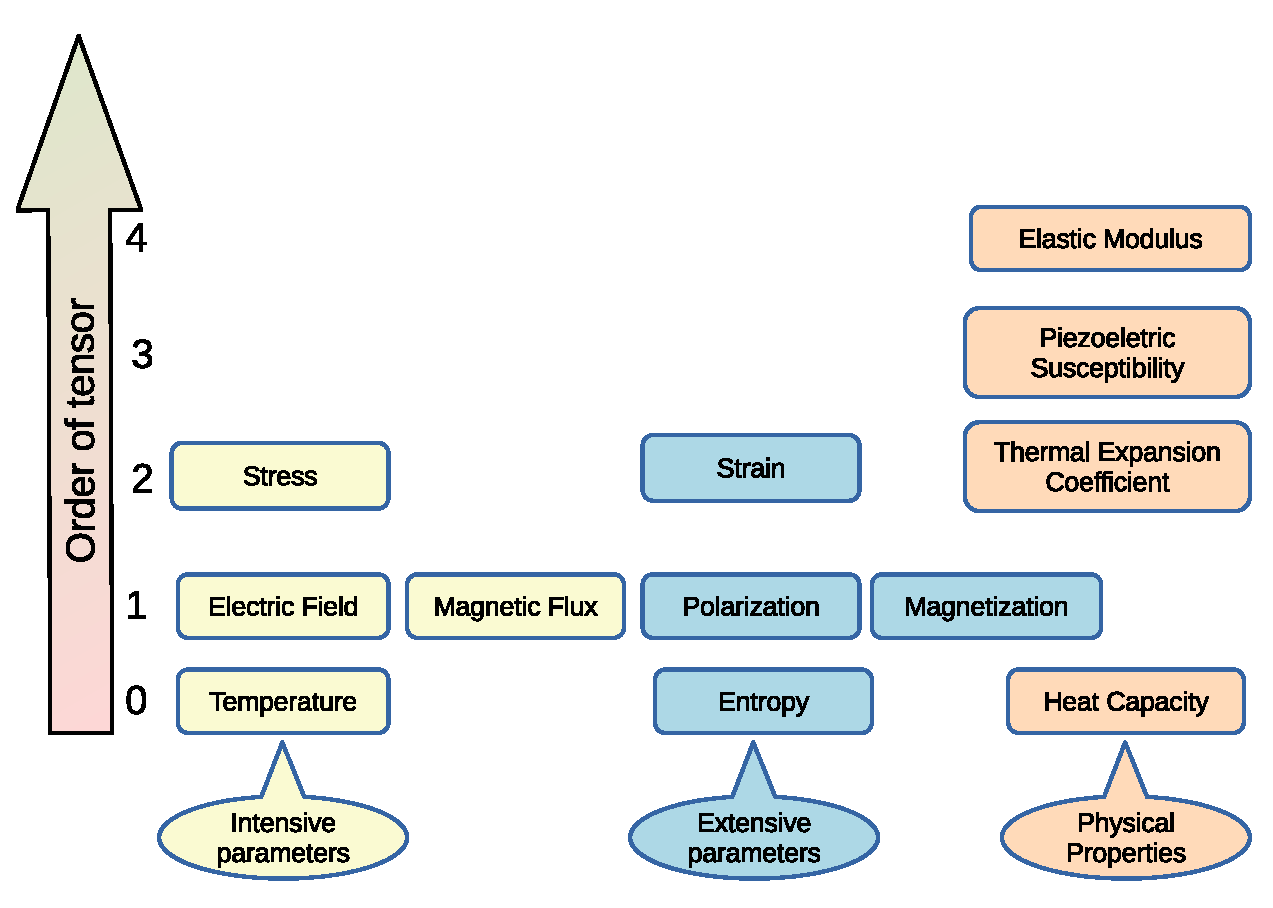
\includegraphics[scale=0.8]{images/c06-tensorexamples.eps}
 }
\end{center}
\caption{Examples of tensor quantities}
\label{tensorexamples}
\end{figure}

{\bf Constitutive relations}

{\bf Definition}
Constitutive relations are those that connect cause and effect.

$$ \text{Effect} = \text{Property} \, \times \, \text{Cause} $$

\begin{itemize}
\item Linear constitutive relations are quite popular.
\end{itemize}

% -----------------------------------------------------------------------

{\bf Heat conduction}

{\bf Fourier's law}
$$\vec{J} = -k \vec{\nabla}T$$

Thermal conductivity $k_{ij}$ is a tensor of order 2 since heat flux $\vec{J}$ and thermal gradient $\vec{\nabla} T$ are vectors.


% -----------------------------------------------------------------------

{\bf Elasticity}

{\bf Hooke's law}
$$ e = C \sigma $$

Compliance $C_{ijkl}$ is a tensor of order 4 since strain $e_{kl}$ and stress $\sigma_{ij}$ are tensors of order 2.


% -----------------------------------------------------------------------

{\bf Viscosity}

{\bf Newton's law}
$$ d_{ij} = \mu_{ijkl} {\partial u_k \over \partial x_l} $$

Viscosity $\mu_{ijkl}$ is a tensor of order 4 since strain rate ${\partial u_k \over \partial x_l}$ and deviatoric stress $d_{ij}$ are tensors of order 2.


% -----------------------------------------------------------------------

{\bf Thermal expansion}

$$ \sigma = \alpha \, \Delta T $$

Thermal expansion coefficient $\alpha_{ij}$ is a tensor of order 2 since stress $\sigma_{ij}$ is a tensor of order 2 and temperature difference $\Delta T$ is a scalar.


% -----------------------------------------------------------------------

{\bf Electrical resistance}

{\bf Ohm's law}
$$ \vec{E} = \rho \, \vec{J} $$

Electrical resistivity $\rho_{ij}$ is a tensor of order 2 since electric field strengh $\vec{E}$ and current density  $\vec{J}$ are vectors.


% -----------------------------------------------------------------------

{\bf Piezoelectric effect}

$$ P_i = d_{ijk} \sigma_{jk} $$

Direct piezeoelectric coefficient $d_{ijk}$ is a tensor of order 3 since polarization $\vec{P}$ is a vector and stress $\sigma_{jk}$ is a tensor of order 2.

Since centrosymmetric crystals cannot have properties of odd rank tensor, such crystals do not exhibit Piezeoelectricity.

% -----------------------------------------------------------------------

{\bf Electrostriction}

$$ x_{ij} = d_{ijk} E_k + M_{ijkl} E_k E_l $$

Direct piezeoelectric coefficient $d_{ijk}$ is a tensor of order 3 since polarization $\vec{P}$ is a vector and stress $\sigma_{jk}$ is a tensor of order 2.

Because of the second term, electrostriction is not limited to non-centrosymmetric crystals.


% -----------------------------------------------------------------------

{\bf Solute diffusion}

{\bf Fick's law}
$$ \vec{J}_A = -D \vec{\nabla} C_A $$

According to Fick's law, diffusion of a species A is down the concentration gradient. Actually it is down the chemical potential gradient. Since flux of species $\vec{J}_A$ and concentration (or chemical potential) gradient $\vec{\nabla} C_A$ (or $\vec{\nabla} \mu_A$) are vectors, diffusivity $D_{ij}$ must be a tensor of order 2.


% -----------------------------------------------------------------------


{\bf Curie Principle}


When certain causes lead to certain effects, the symmetry elements of the causes should be observed in these effects.


% -----------------------------------------------------------------------

{\bf Neumann Principle}

The symmetry of any physical property of a crystal must include the symmetry elements of the point group of the crystal.

% -----------------------------------------------------------------------

{\bf Symmetry effects on property tensors}

\begin{itemize}
\item Gases : Isotropic  
\item Liquids : Isotropic
\item Polycrystalline solids : Isotropic
\item Textured solids : Anisotropic, depending on type of texture
\item Single crystals : Anisotropic, depending on crystal symmetry
\end{itemize}

% -----------------------------------------------------------------------

% learning objective
\begin {lo3} [Tensors]
List number of independent components and the form of isotropic tensors
\end {lo3}

\section{Isotropic tensors}

\index{Tensor, isotropic}

{\bf Definition:} A tensor is isotropic if its elements donot change under {\em any} co-ordinate transformation\footnote{involving only rotations and reflections but not expansions or contractions ie., Det($T_{ij}$) is unity}.

\begin{itemize}

\item
Kronecker delta is an isotropic tensor of order two. The general form of an isotropic tensor of order two is 
$$ a_{ij} = a \delta_{ij}$$

\item
Levi-Civita density is an isotropic tensor of order three. Proof is given in section \ref{levicivitaisotropic} It is also referred to as alternating tensor or permutation tensor.

Relation between $\epsilon_{ijk}$ and $\delta_{ij}$ and the proof are given in equation \ref{epsilondelta}.

\item
$\delta_{ij}\delta_{kl}$ is an isotropic tensor of order four.

Most general form of an isotropic tensor of order four, where $\mu_1$, $\mu_2$ and $\mu_3$ are constants:

\begin{equation}
\boxed{\mu_{ijkl} = \mu_1\delta_{ij}\delta_{kl} + \mu_2\delta_{ik}\delta_{jl} + \mu_3\delta_{il}\delta_{jk}}
\end{equation} 

Proof is given in section \ref{isotensorfour}.

\end{itemize}


{\bf General forms of isotropic tensors for properties}

\begin{itemize}
\item Isotropic tensor of order 2 : $$\lambda \, \delta_{ij}$$
\item Isotropic tensor of order 3 : $$\lambda \, \epsilon_{ijk}$$
\item Isotropic tensor of order 4 : $$\lambda_1 \, \delta_{ij} \delta_{kl} + \lambda_2 \, \delta_{il} \delta_{kj} + \lambda_3 \, \delta_{ik} \delta_{jl}$$
\end{itemize}


% -----------------------------------------------------------------------

{\bf Imposing symmetry on property tensor}

If $a$ is a property tensor of order 2, use the following expression to identify the minimum number of elements of $a$ needed to represent it.
$$ a_{pq} = T_{pi} T_{qj} a_{ij} $$
Where $T_{pi}$ is the matrix corresponding to a coordinate transformation that represents a symmetry operation.

% -----------------------------------------------------------------------

\section{Symmetry elements of crystal classes}
Herrmann-Mauguin symbol is used for crystal class.


\begin{table}[h!]
\begin{tabular}{lll}
\hline \\
Crystal System & Crystal Class & Symmetry Elements \\
\hline \\
Monoclinic &  $2$ & $2 \parallel Z_2$ \\
Orthorhombic &  $222$ & $2 \parallel Z_1$ , $2 \parallel Z_2$ \\
Tetragonal & $\bar{4}2m$ & $\bar{4} \parallel Z_3$ , $2 \parallel Z_1$ \\
Hexagonal & $6/mmm$ & $6 \parallel Z_3$, $m \bot Z_3$, $m \bot Z_1$ \\
Cubic & $\bar{4}3m$ & $\bar{4} \parallel Z_3$, $3 \parallel [111]$ \\
\hline \\
\end{tabular}
\caption{Symmetry elements in some crystal systems}
\label{table:2}
\end{table}

% -----------------------------------------------------------------------

% learning objective
\begin {lo3} [Tensors]
Determine a transformation matrix suitable for a symmetry operation
\end {lo3}

{\bf Transformation matrices for symmetry operations}

Twofold rotation $2 \parallel Z_1$
\begin{equation*}
\left[
\begin{array}{lll}
1 & 0 & 0 \\
0 & -1 & 0 \\
0 & 0 & -1 \\
\end{array}
\right]
\end{equation*}

Mirror $m \bot Z_1$ 
\begin{equation*}
\left[
\begin{array}{lll}
-1 & 0 & 0 \\
0 & 1 & 0 \\
0 & 0 & 1 
\end{array}
\right]
\end{equation*}

Threefold rotation $3 \parallel Z_3$
\begin{equation*}
\left[
\begin{array}{lll}
-{1 \over 2} & {\sqrt{3} \over 2} & 0 \\
-{\sqrt{3} \over 2} & -{1 \over 2} & 0 \\
0 & 0 & 1 
\end{array}
\right]
\end{equation*}
Threefold rotation $3 \parallel [111]$
\begin{equation*}
\left[
\begin{array}{lll}
0 & 1 & 0 \\
0 & 0 & 1 \\
1 & 0 & 0 
\end{array}
\right]
\end{equation*}

Fourfold rotation $4 \parallel Z_3$
\begin{equation*}
\left[
\begin{array}{lll}
0 & 1 & 0 \\
-1 & 0 & 0 \\
0 & 0 & 1 
\end{array}
\right]
\end{equation*}

Fourfold inversion $\bar{4} \parallel Z_3$
\begin{equation*}
\left[
\begin{array}{lll}
0 & -1 & 0 \\
1 & 0 & 0 \\
0 & 0 & -1 
\end{array}
\right]
\end{equation*}


% -----------------------------------------------------------------------

{\bf Most property tensors are symmetric}

{\bf Microscopic Reversibility Principle}
For a system in thermodynamic equilibrium, every type of micromotion occurs just as often as its reverse.

{\bf Onsager's Reciprocity Principle}
Provided a proper choice is made for the fluxes and affinities, the matrix of phenomenological coefficients is symmetrical

As an implication of this, thermal conductivity $k_{ij}$ is a symmetric tensor.


% -----------------------------------------------------------------------
% learning objective
\begin {lo3} [Tensors]
Apply symmetry principles to reduce the number of independent components of a property tensor
\end {lo3}

\section{Scaffold to reduce components by symmetry operations}

\begin{mdframed}[style=tpscaffold1]
A crystal has a property $k_{ij}$ which is known to be a symmetric tensor of order 2. 

\begin{enumerate}
\item Write down the matrix representation of this tensor in its most general form.
\item If the crystal were to be rotated by 90 degrees, anti-clockwise about the $z$-axis, write down the new unit vectors in terms of the old unit vectors.
\item Looking at the above three relations, write down the transformation matrix $T$.
\item Determine the expression for the $k^*_{11}$ component of this tensor property in the new coordinate system.
\item Determine the expression for the $k^*_{21}$ component of this tensor property in the new coordinate system.
\item What does it mean to say $k^*_{11} = k_{11}$? or to say $k^*_{21} = k_{21}$?
\item If $k^*_{11} = k_{11}$, what can you infer?
\item If $k^*_{21} = k_{21}$, what can you infer?
\item If a four fold rotational symmetry is all that this crystal possesses, what can you say about the simplest form of $k$? Which crystal system would such a symmetry correspond to?
\item Extend the above steps for two other four fold rotations and arrive at the simplest possible form for $k$ for a cubic crystal.
\end{enumerate}
\end{mdframed}

{\bf Applying symmetry to property tensor}

Thermal conductivity $k_{ij}$, a second order symmetric tensor.
\begin{equation*}
k_{ij} = \left[
\begin{array}{lll}
k_{11} & k_{12} & k_{13} \\
k_{12} & k_{22} & k_{23} \\
k_{13} & k_{23} & k_{33}
\end{array}
\right]
\end{equation*}

Take the symmetry operation of 4 fold rotation (by $90^o$) about $\hat{x}_3$. Corresponding transformation matrix is:
\begin{equation*}
T = \left[
\begin{array}{lll}
0 & 1 & 0 \\
-1 & 0 & 0 \\
0 & 0 & 1
\end{array}
\right] 
\end{equation*}


Combining Neumann Principle and the definition of a second order tensor,
$$ k_{pq} = T_{pi} T_{qj} k_{ij} $$
\begin{enumerate}
\item Pick a combination of $p \, \& \, q$
\item Expand RHS, knowing not all terms of T are non-zero.
\item Repeat for all possible symmetry operations
\end{enumerate}


Using : $T_{12} = T_{33} = 1$, $T_{21}=-1$ and $ k_{pq} = T_{pi} T_{qj} k_{ij} $
$$k_{11} = T_{1i}T_{1j}k_{ij} = T_{12} T_{12} k_{22} = k_{22} \implies k_{11} = k_{22}$$

Similarly,
$$k_{21} = T_{2i} T_{1j} k_{ij} = T_{21} T_{12} k_{12} = -k_{12} = -k_{21} \implies k_{21} = k_{12} = 0$$

Using remaining symmetry operations, one can see that all off diagonal terms of $k_{ij}$ vanish and all diagonal terms are same.
\begin{equation*}
k_{ij} = \left[
\begin{array}{lll}
k_{11} & 0 & 0 \\
0 & k_{11} & 0 \\
0 & 0 & k_{11}
\end{array}
\right] = k_{11} \delta_{ij}
\end{equation*}


% -----------------------------------------------------------------------

\section{Components of a symmetric tensor property}

Triclinic:
\begin{equation*}
\left[
\begin{array}{lll}
S_{11} & S_{12} & S_{13} \\
 & S_{22} & S_{23} \\
 &  & S_{33} \\
\end{array}
\right]
\end{equation*}

Monoclinic:
\begin{equation*}
\left[
\begin{array}{lll}
S_{11} & 0 & S_{13} \\
 & S_{22} & 0 \\
 &  & S_{33} \\
\end{array}
\right]
\end{equation*}

Orthorhombic:
\begin{equation*}
\left[
\begin{array}{lll}
S_{11} & 0 & 0 \\
 & S_{22} & 0 \\
 &  & S_{33} \\
\end{array}
\right]
\end{equation*}

Tetragonal, trigonal, hexagonal:
\begin{equation*}
\left[
\begin{array}{lll}
S_{11} & 0 & 0 \\
 & S_{11} & 0 \\
 &  & S_{33} \\
\end{array}
\right]
\end{equation*}

Cubic:
\begin{equation*}
\left[
\begin{array}{lll}
S_{11} & 0 & 0 \\
 & S_{11} & 0 \\
 &  & S_{11} \\
\end{array}
\right]
\end{equation*}

% -----------------------------------------------------------------------

{\bf Diagonalizability theorem}

\begin{itemize}

\item There exists a coordinate system in which a symmetric tensor can be represented only by diagonal elements.
\item Stress is a symmetric tensor because of continuum approximation.
\item This is used to arrive at the principal components of a stress state.
\end{itemize}

% ---------------------------------------------------------------------

\section{Summary}

\begin{enumerate}
\item Kronecker delta $\delta_{ij}$ can be used: to simplify subscripts, $a_{ik} \delta_{ij} = a_{jk}$, to represent inner / dot products and to represent an isotropic tensor of order two.
\item Levi-Civita / permutation matrix can be used: to represent cross products, to arrive at determinants of matrices and to represent an isotropic tensor of order three.
\item Kronecker delta and Levi-Civita symbol are connected as: $\epsilon_{ijk} \epsilon_{klm} = \delta_{il} \delta_{jm} - \delta_{im} \delta_{jl}$ and $\epsilon_{ijk} \epsilon_{ijm} = 2 \delta_{km}$.
\end{enumerate}

% ---------------------------------------------------------------------

% -------------------------------
% Fluid Flow
% -------------------------------
\chapter{Continuity Equation}
\label{ch:continuity}

\section{Learning objectives}
At the end of this chapter, a student should be able to 
\begin{enumerate}
\item apply continuity equation to determine unknown components of a velocity field
\item plot stream function as contours to visualize flow field in a 2D domain
\end{enumerate}

% learning objective
\begin {lo3} [Fluid Flow]
Derive continuity equation
\end {lo3}

\section{Concept map}
\index{Concept map, material derivative}

\begin{figure}[h]
\begin{center}
\framebox{
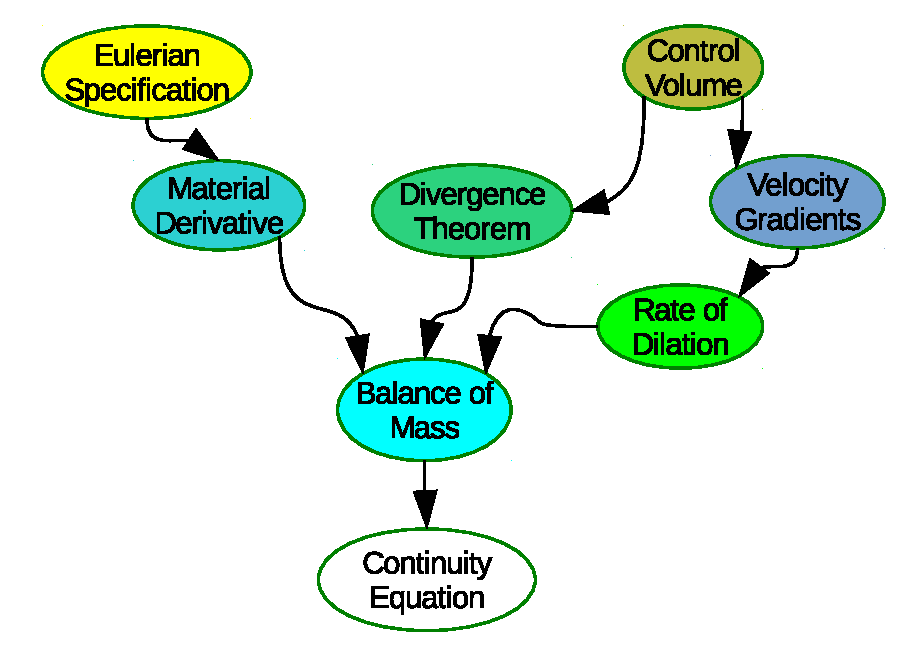
\includegraphics[scale=0.8]{images/c07-MaterialDerivativeFlowChart.eps}
 }
\end{center}
\caption{Concept map to arrive at continuity equation}
\label{ContinuityEquationConceptMap}
\end{figure}

A concept map that exposes the connections between different concepts behind continuity equation is given in the figure~\ref{ContinuityEquationConceptMap}.

% -----------------------------------------------------------------------

\section{Type of specifications}

\begin{figure}[h]
\begin{center}
\framebox{
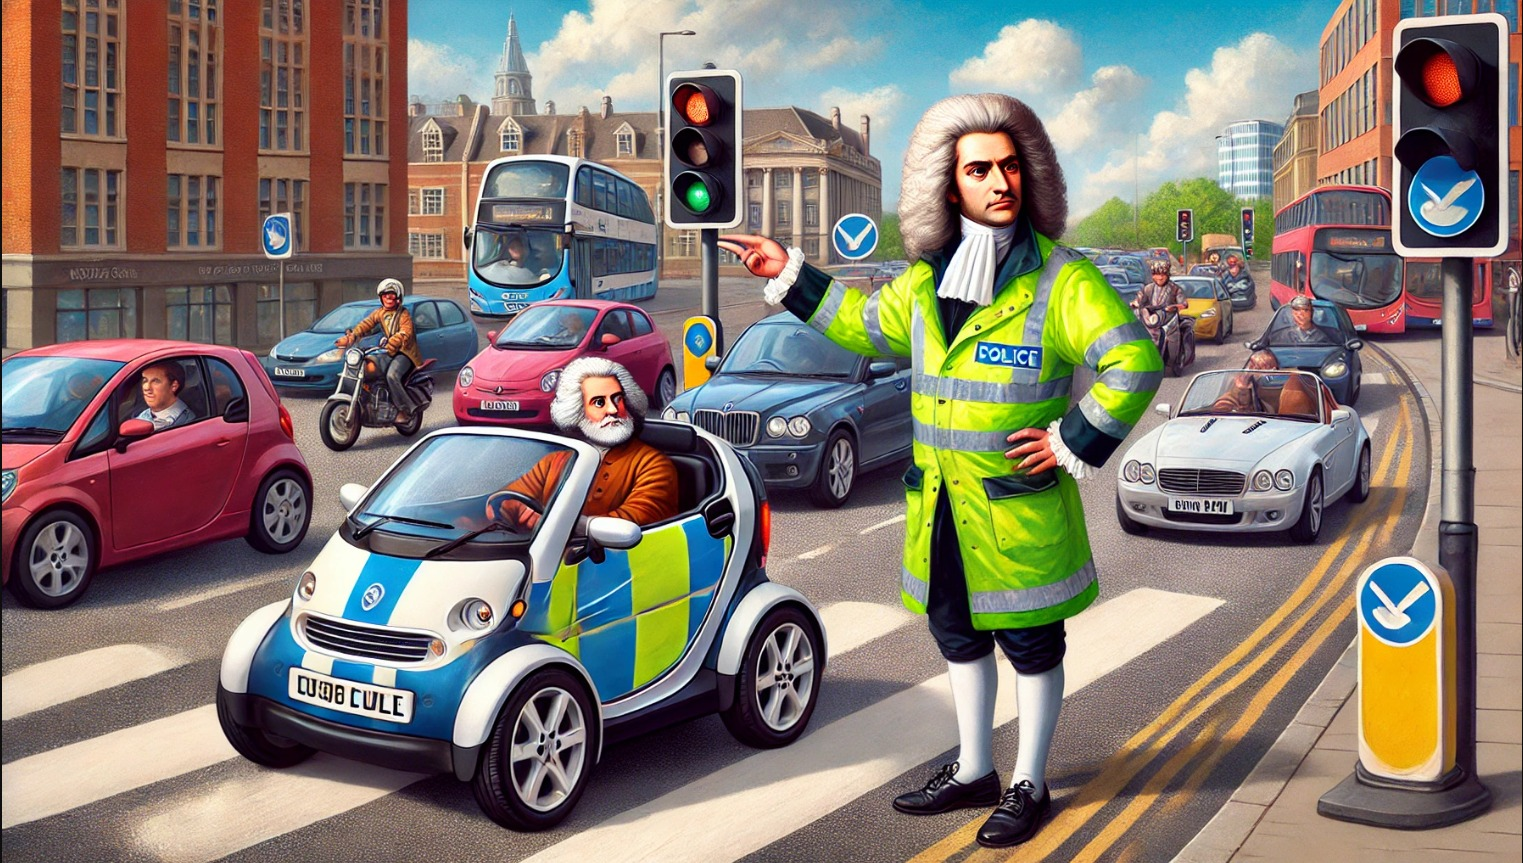
\includegraphics[scale=0.8]{images/c07-eulerlagrange.eps}
 }
\end{center}
\caption{An image generated by chatgpt to show Euler as traffic police and Lagrange as a driver. Helps connect the specifications to the respective perspectives}
\label{eulerlagrange}
\end{figure}


Figure~\ref{VolumeElementMotion} illustrates a control volume being advected in a fluid. Consider a parameter that can be specified at the center of this control volume. Time derivative of such a parameter could be described either in a coordinate system fixed to the center of the control volume itself or in an external coordinate system of the observer.

\begin{figure}[h]
\begin{center}
\framebox{
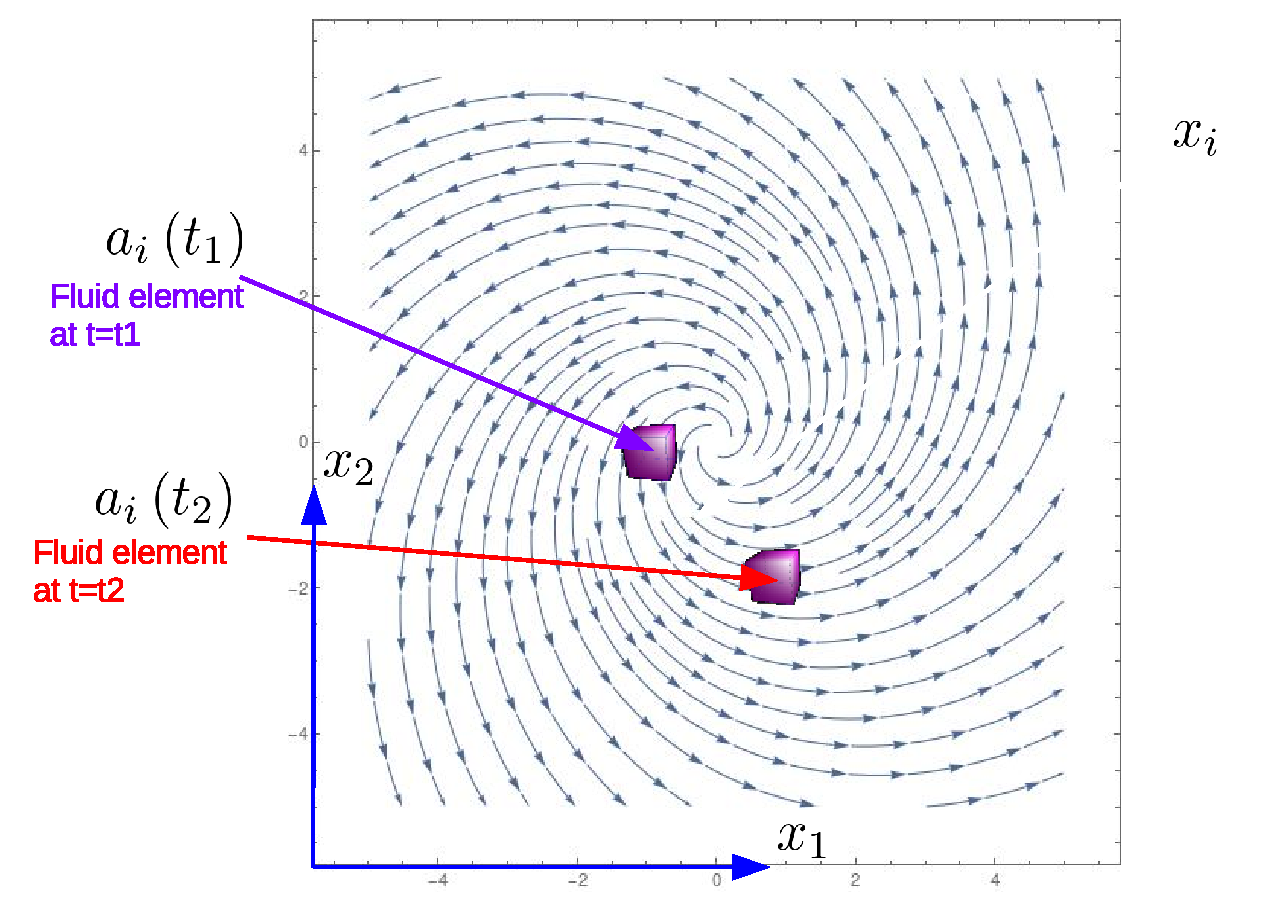
\includegraphics[scale=0.5]{images/c07-VolumeElementMotion.eps}
 }
\end{center}
\caption{Motion of a volume element in a fluid}
\label{VolumeElementMotion}
\end{figure}


% -----------------------------------------------------------------------


{\bf Lagrangian}:
Velocities are specified at the centre of mass ($a_i$) and time ($t$).

{\bf Eulerian}:
Velocities are specified in terms of position ($x_i$) and time ($t$).

\begin{itemize}
\item Eulerian specification gives spatial gradients of velocities directly.
\item Lagrangian specification helps trace the path of an element directly.
\end{itemize}


% -----------------------------------------------------------------------

\section{Time derivative}

\index{Eulerian specification}
Consider a flow field and trace a particle that moves with the flow. The flow field can be specified in two ways. In the {\bf Eulerian} type of specification, the velocities are specified in terms of position ($x_i$) and time ($t$). It gives the spacial distribution of velocity $u_i(x_i,t)$ similar to density, temperature and pressure at any given instant. 

\index{Lagrangian specification}
In {\bf Lagrangian} type of specification, the dynamical history of a specific piece of material (fluid element) is given. The flow field of the element is given in terms of the position (of the center of mass) of the element and time as $v_i(a_i,t)$. 

Eulerian specification gives spacial gradients of velocities directly. Lagrangian specification helps trace the path of an element directly. Unless otherwise specified, one usually uses to the Eulerian frame of reference.

In the Lagrangian specification, since the velocity $v_i(a_i, t)$ is specified at the centre of gravity of the fluid element, acceleration of a fluid element is given by

\begin{equation}
\frac{dv_i}{dt} = \frac{\partial v_i}{\partial t} 
\end{equation} 

In the Eulerian specification, since the velocity ($u_i(x_i,t)$) is specified in terms of the absolute position where as the location of the fluid element changes as dictated by the flow  (see section \ref{variablechange}), acceleration of the fluid element is given as below:

\begin{equation}
\frac{du_i}{dt} = \frac{\partial u_i}{\partial t} + u_i \frac{\partial u_j}{\partial x_j} = \frac{\partial u_i}{\partial t} + u_j \nabla_j u_i 
\end{equation} 

or

\begin{equation}
\frac{d\vec{u}}{dt} = \frac{\partial \vec{u}}{\partial t} + (\vec{u} \cdot \vnabla) \vec{u} 
\end{equation} 

Proof of the same is given in section \ref{materialderivative}.

We now define the {\bf material derivative} which is a time derivative following the motion of the fluid as 

\begin{equation}
\boxed{\frac{D}{Dt} = \frac{\partial}{\partial t} + (\vec{u} \cdot \vnabla) }
\end{equation} 


{\bf Lagrangian}:
$$ {d \phi \over d t} = {\partial \phi \over \partial t} $$

{\bf Eulerian}:
$$ {d \phi \over d t} = {\partial \phi \over \partial t} +  {\partial \phi \over \partial x_1} {\partial x_1 \over \partial t} + {\partial \phi \over \partial x_2} {\partial x_2 \over \partial t} + {\partial \phi \over \partial x_3} {\partial x_3 \over \partial t} $$
$$ = {\partial \phi \over \partial t} +  {\partial \phi \over \partial x_1} u_1 + {\partial \phi \over \partial x_2} u_2 + {\partial \phi \over \partial x_3} u_3 $$
$$ = \left[ {\partial \over \partial t} +  u_1 {\partial \over \partial x_1} + u_2 {\partial \over \partial x_2} + u_3 {\partial \over \partial x_3} \right] \phi $$
$$ {d \phi \over d t} = \left[ {\partial \over \partial t} + \vec{u} \cdot \vec{\nabla} \right] \phi $$

% -----------------------------------------------------------------------

{\bf Acceleration}

{\bf Lagrangian}:
$$ {d \vec{V} \over d t} = {\partial \vec{V} \over \partial t} $$

{\bf Eulerian}:
$$ {d \vec{u} \over d t} = \left[ {\partial \over \partial t} + \vec{u} \cdot \vec{\nabla} \right] \vec{u} $$

% -----------------------------------------------------------------------


{\bf Material derivative}:

$$ {D \over D t} \equiv {\partial \over \partial t} + \vec{u} \cdot \vec{\nabla} \equiv {\partial \over \partial t} + u_j \nabla_j $$

% -----------------------------------------------------------------------

\section{Flux of mass}

{\bf Convention for flux}:

\begin{figure}[h]
\begin{center}
\framebox{
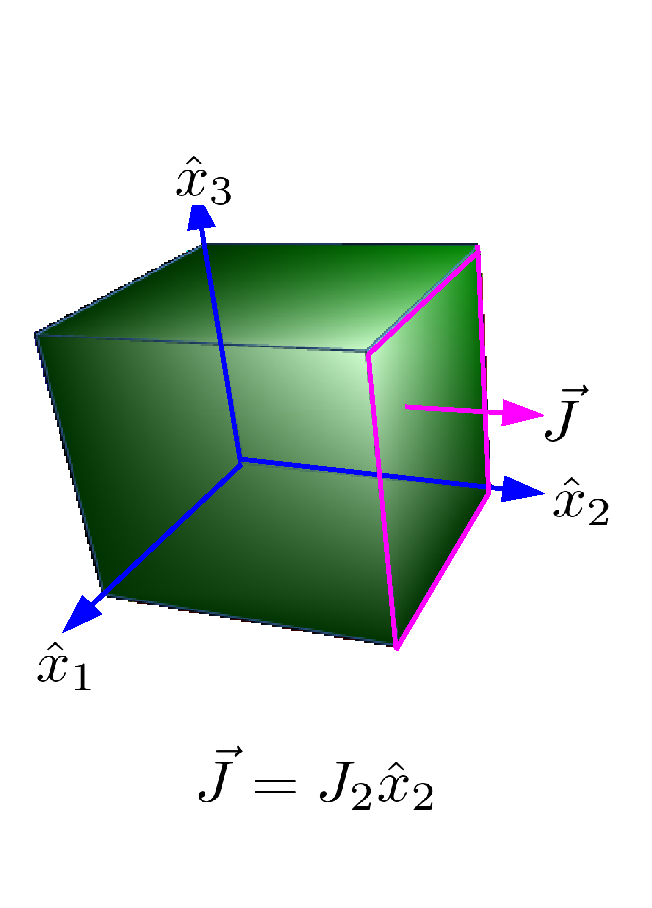
\includegraphics[scale=0.5]{images/c07-FluxConvention.eps}
 }
\end{center}
\caption{Convention for flux of material}
\label{FluxConvention}
\end{figure}


Area element has {\bf outward} normal.
$$ \vec{dS} = dA \, \hat{n} $$
$$ \vec{dS} = dx_1 \, dx_3 \, \hat{x}_2 $$
Mass flux:
$$ \vec{J} = \rho \vec{u} $$
$$ J_2 = \rho u_2 $$
Mass flow rate through the area element:
$$ \vec{J} \cdot \vec{dS} = \rho u_2 \, dx_1 \, dx_3 $$

% -----------------------------------------------------------------------

{\bf Divergence theorem}:

\begin{figure}[h]
\begin{center}
\framebox{
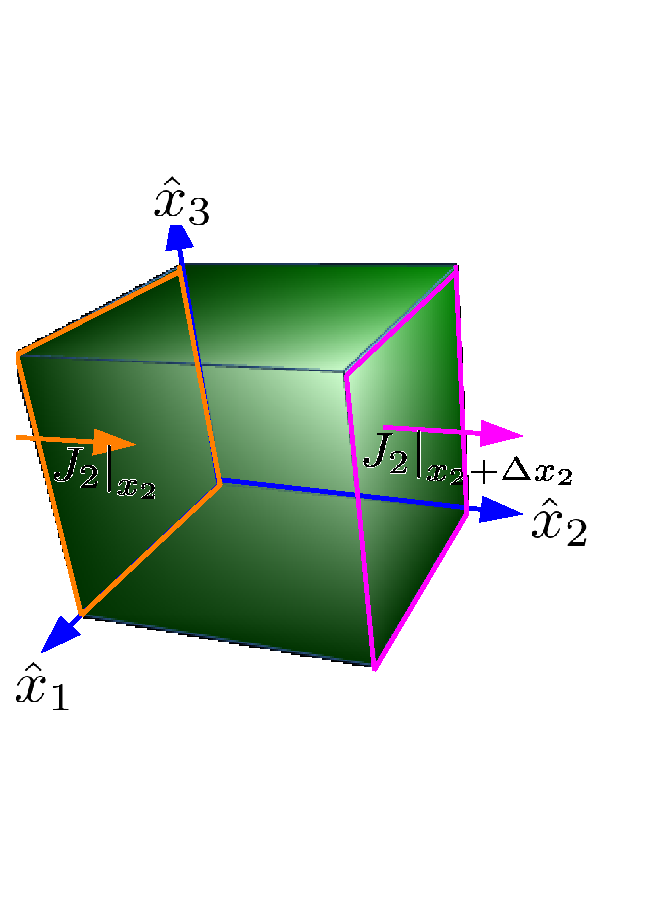
\includegraphics[scale=0.5]{images/c07-DivergenceTheorem.eps}
 }
\end{center}
\caption{Schematic for divergence theorem}
\label{DivergenceSchematic}
\end{figure}

Consider for 6 faces of the volume element:
$$ \sum{\vec{J} \cdot \vec{dS}} $$

Total outward mass flow:
$$ \left. J_2 \right|_{x_2+\Delta x_2} \Delta x_1 \Delta x_3 - \left. J_2 \right|_{x_2} \Delta x_1 \Delta x_3 $$
$$ + \left. J_3 \right|_{x_3+\Delta x_3} \Delta x_1 \Delta x_2 - \left. J_3 \right|_{x_3} \Delta x_1 \Delta x_2 $$
$$ + \left. J_1 \right|_{x_1+\Delta x_1} \Delta x_2 \Delta x_3 - \left. J_1 \right|_{x_1} \Delta x_2 \Delta x_3 $$
$$ = \left[ { \partial J_1 \over \partial x_1} + { \partial J_2 \over \partial x_2} + { \partial J_3 \over \partial x_3}  \right] \Delta x_1 \Delta x_2 \Delta x_3 $$
$$ \Delta V = \Delta x_1 \, \Delta x_2 \, \Delta x_3 $$


% -----------------------------------------------------------------------

{\bf Divergence theorem}:

$$ \sum{\vec{J} \cdot \vec{dS}} = \left[ \vec{\nabla} \cdot \vec{J} \right] \Delta V $$
$$ \int_{s}{\vec{J} \cdot \vec{dS}} = \int_{v}{\vec{\nabla} \cdot \vec{J} dV} $$ 
$$ \int_{s}{J_i \, n_i \, dS} = \int_{v}{ {\partial J_i \over \partial x_i} dV} $$ 

% -----------------------------------------------------------------------

\section{Mass balance}

{\bf Statement in words}:
Total influx of mass into a control volume equals increase in its mass.

As per our convention, $\vec{dS}$ is outward normal to the face of the control volume. So $\int_{s}{\vec{J} \cdot \vec{dS}}$ is total outflux.

Increase in mass of a control volume fixed in space is $\int_{v}{{\partial \rho \over \partial t} dV}$.

{\bf Statement for a CV }
$$\int_{v}{{\partial \rho \over \partial t} dV} = - \int_{s}{\vec{J} \cdot \vec{dS}}$$


% -----------------------------------------------------------------------

\section{Continuity equation}

Consider a control volume of surface area $S$ and volume $V$ though which a flow $\vec{u}$ is taking place. Conservation of mass requires that the increase in amount of fluid in the element is equal to the amount brought in by the fluid flow (in the absence of sources and sinks that are singular). By convention, the surface normal $\vec{n}$ points {\em outwards} and hence the conservation can be written as follows.

Mass balance over a control volume fixed in space:

\begin{equation}
	\int_{V}{\frac{\partial \rho}{\partial t} dV} = -\int_{S}{\vec{J} \cdot\vec{n}dS} = -\int_{S}{\left( \rho\vec{u} \right) \cdot\vec{n}dS}
\end{equation} 

$$ \int_{v}{{\partial \rho \over \partial t} dV} = - \int_{s}{\vec{J} \cdot \vec{dS}} = - \int_{v}{\vec{\nabla} \cdot \vec{J} dV} = - \int_{v}{\vec{\nabla} \cdot \left(\rho \vec{u} \right) dV} $$

Expanding the RHS,

$$ \int_{v}{{\partial \rho \over \partial t} dV} = - \rho \int_{v}{\vec{\nabla} \cdot \vec{u} dV} - \int_{v}{ \vec{u} \cdot \vec{\nabla} \rho dV} $$

$$ \int_{v}{\left[{\partial \rho \over \partial t} + \vec{u} \cdot \vec{\nabla} \rho\right] dV} = - \int_{v}{ \rho \vec{\nabla} \cdot \vec{u} dV} $$


Using the Gauss theorem\footnote{Actually Gauss-Ostrogradsky theorem} to convert the surface integral to volume integral,

\begin{equation}
\int_{V}{\frac{\partial \rho}{\partial t} dV} = -\int_{V}{\vnabla\cdot(\rho\vec{u})dV}
\end{equation} 

For this relation to be valid at {\em all} locations in the fluid,


\begin{equation}
\label{conteq1}
\boxed{\frac{\partial \rho}{\partial t} +  \vnabla\cdot(\rho\vec{u}) = 0}
\end{equation}


Use the identity in question~\ref{divsv} to expand the above equation as

\begin{equation}
\frac{\partial \rho}{\partial t} + (\vec{u}\cdot\vnabla)\rho + \rho\vnabla\cdot\vec{u}  = 0
\end{equation} 

Identifying the definition of material derivative $\frac{D}{Dt}$ and dividing by $\rho$,

\begin{equation}
\label{conteq2}
\boxed{\frac{1}{\rho}\frac{D \rho}{D t} + \vnabla\cdot\vec{u}  = \frac{1}{\rho}\frac{D \rho}{D t} + \Delta = 0}
\end{equation} 

\index{Rate of dilation}
\index{Compressibility}
\index{Rate of expansion}
$\vnabla\cdot\vec{u}$ is called as {\em rate of dilation} or rate of expansion or compressibility and is indicated by a symbol $\Delta$.

\begin{equation}
\label{rdiln}
\Delta = \vnabla\cdot\vec{u}  = \nabla_i u_i = u_{i,i}
\end{equation} 

Equations \ref{conteq1} and \ref{conteq2} are two alternate forms of the {\em continuity equation}.

\index{Incompressible fluid}
A fluid is called as {\em incompressible} if the density does not change due to changes in pressure (or) if the rate of change of density following the flow is zero. For {\em incompressible} fluids, the continuity equation reduces to:

\begin{equation}
\vnabla\cdot\vec{u}  = \Delta = 0
\end{equation} 

Sections \ref{variablechange} and \ref{materialderivative} state the same thing more rigorously.

% -----------------------------------------------------------------------

\section{Strain rate tensor}

The way velocity gradients would change the shape of a moving control volume in a fluid is illustrate in the following figures.

\begin{figure}[h]
\begin{center}
\framebox{
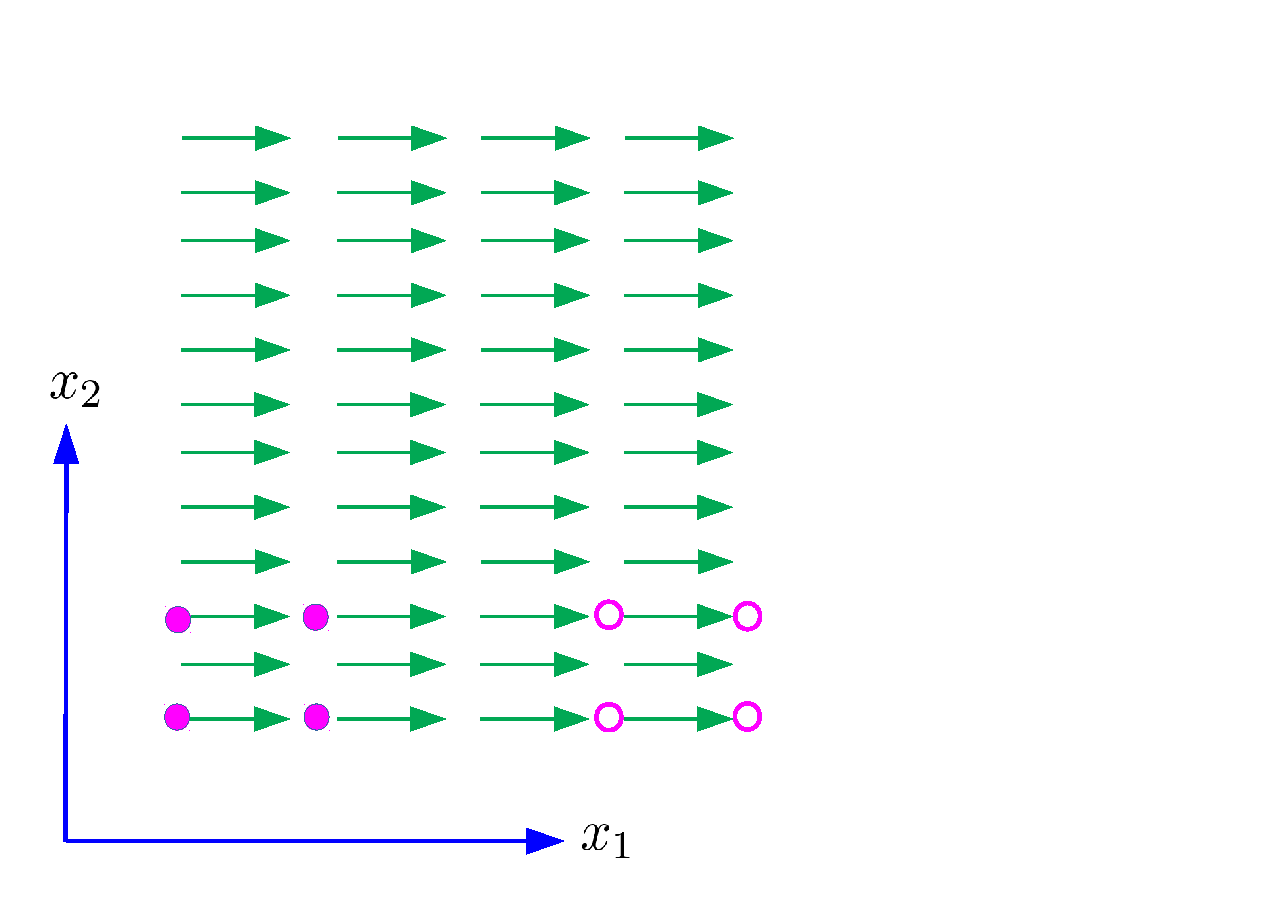
\includegraphics[scale=0.5]{images/c07-CVTranslate1.eps}
 }
\end{center}
\caption{Motion of a control volume due to unidirectional flow along $\hat{x}_1$}
\label{CVTranslation1}
\end{figure}


% -----------------------------------------------------------------------

\begin{figure}[h]
\begin{center}
\framebox{
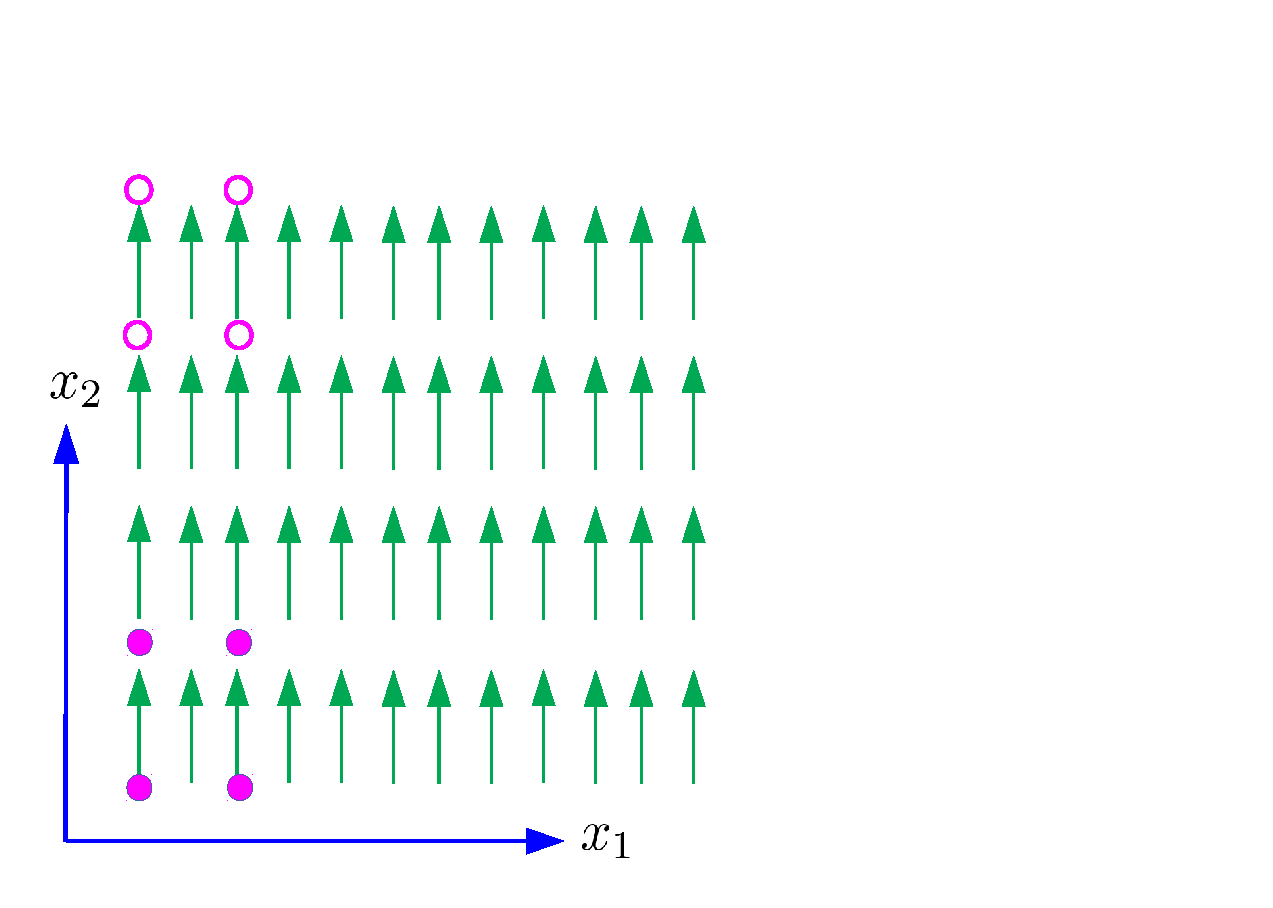
\includegraphics[scale=0.5]{images/c07-CVTranslate2.eps}
 }
\end{center}
\caption{Motion of a control volume due to unidirectional flow along $\hat{x}_2$}
\label{CVTranslation2}
\end{figure}


% -----------------------------------------------------------------------

\begin{figure}[h]
\begin{center}
\framebox{
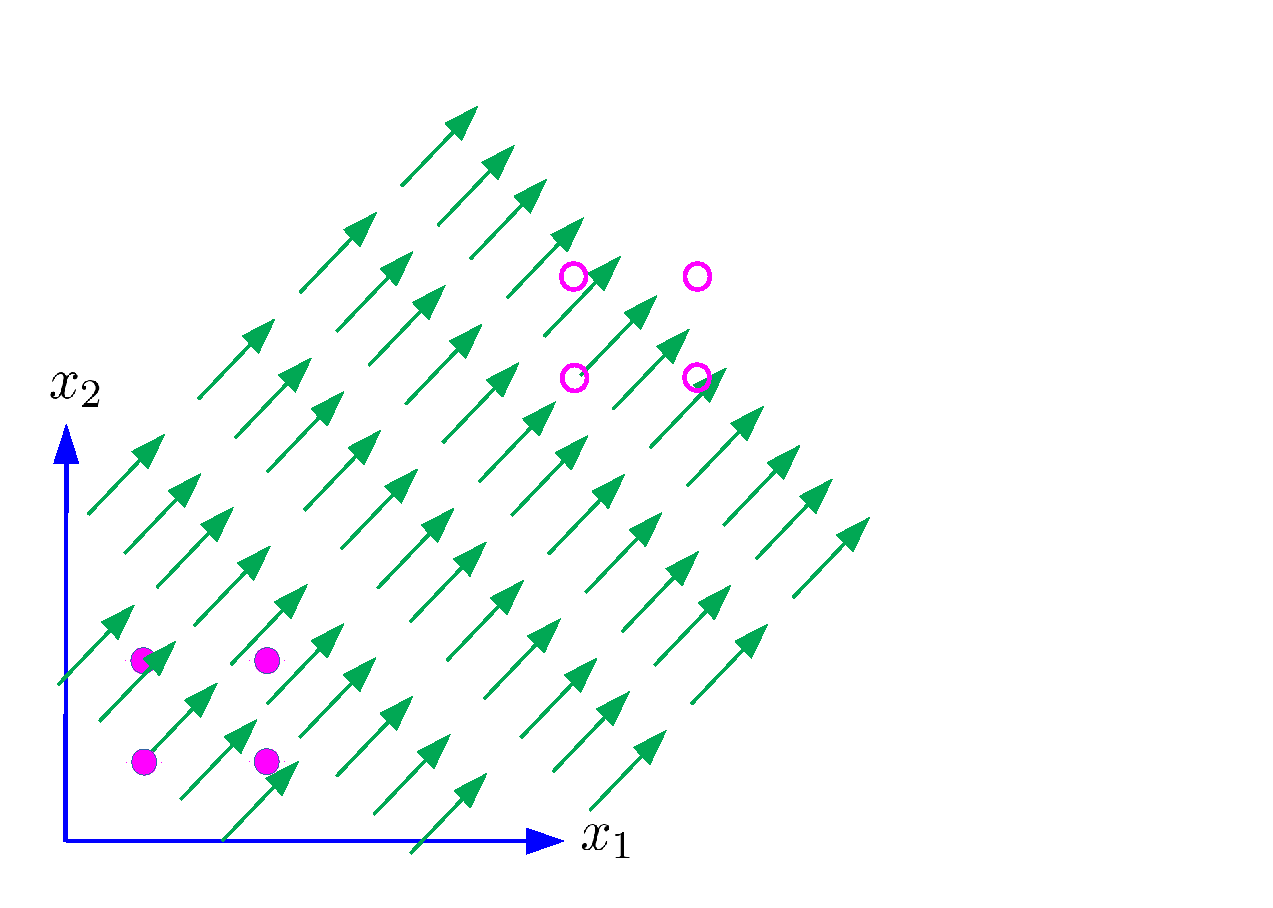
\includegraphics[scale=0.5]{images/c07-CVTranslate3.eps}
 }
\end{center}
\caption{Motion of a control volume due to unidirectional flow}
\label{CVTranslation3}
\end{figure}

% -----------------------------------------------------------------------

\begin{figure}[h]
\begin{center}
\framebox{
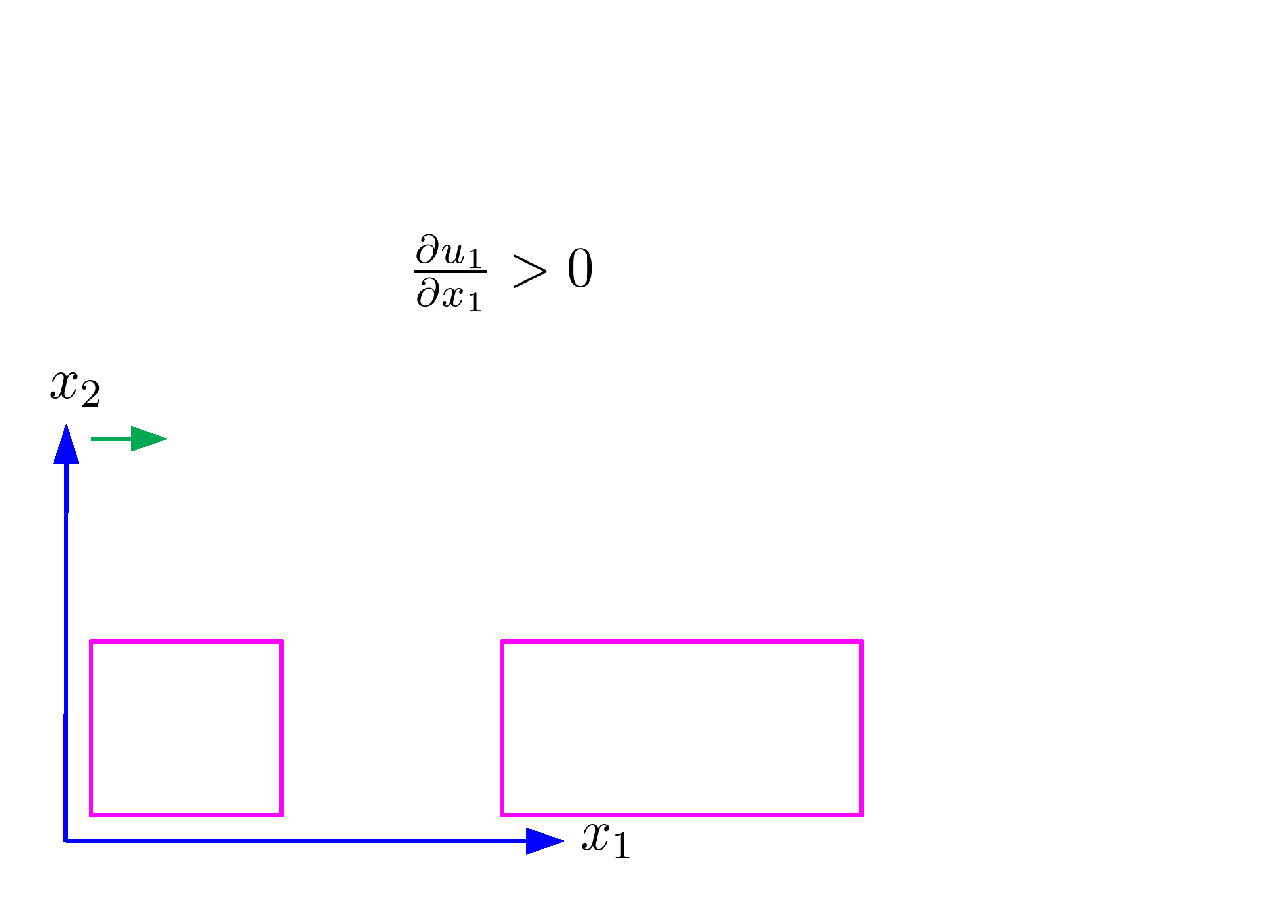
\includegraphics[scale=0.5]{images/c07-CVTranslate4.eps}
 }
\end{center}
\caption{Motion of a control volume due to flow with velocity gradient}
\label{CVTranslation4}
\end{figure}

From the figures, it is clear that uniform velocities lead to only translation of a control volume but velocity gradients would change the shape.

% -----------------------------------------------------------------------

\begin{equation*}
{\partial u_i \over \partial x_j} = 
\left[
\begin{array}{lll}
{\partial u_1 \over \partial x_1} & {\partial u_1 \over \partial x_2} & {\partial u_1 \over \partial x_3} \\
\\
{\partial u_2 \over \partial x_1} & {\partial u_2 \over \partial x_2} & {\partial u_2 \over \partial x_3} \\
\\
{\partial u_3 \over \partial x_1} & {\partial u_3 \over \partial x_2} & {\partial u_3 \over \partial x_3} \\
\end{array}
\right]
\end{equation*}

Changes to a fluid element:
\begin{enumerate}
\item Translation
\item Dilation
\item Shear
\item Rotation
\end{enumerate}

% -----------------------------------------------------------------------

\section{Rate of dilation}

\begin{figure}[h]
\begin{center}
\framebox{
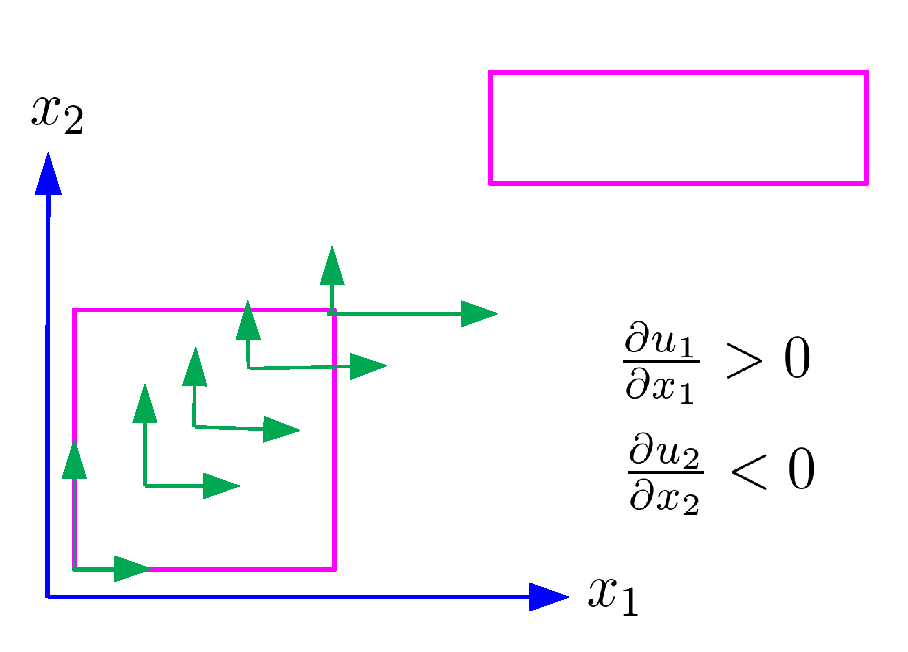
\includegraphics[scale=0.5]{images/c07-CVTranslate5.eps}
 }
\end{center}
\caption{Rate of dilation}
\label{CVTranslation5}
\end{figure}

Define rate of dilation as:
$$ \Delta = \vec{\nabla} \cdot \vec{u} $$
$$ \Delta = \text{Trace of} \, {\partial u_i \over \partial x_j} $$

% -----------------------------------------------------------------------

\section{Other forms of continuity equation}

$$ {1 \over \rho} {D \rho \over D t} + \Delta = 0 $$

We define an {\bf incompressible fluid} as follows:
$$ {1 \over \rho} {D \rho \over D t} = 0 $$

Continuity equation of an incompressible fluid:
$$ \Delta = \vec{\nabla} \cdot \vec{u} = {\partial u_1 \over \partial x_1} + {\partial u_2 \over \partial x_2} + {\partial u_3 \over \partial x_3} = 0 $$

% -----------------------------------------------------------------------

{\bf Continuity equation}: 
For incompressible fluids:
$$\vec{\nabla} \cdot \vec{u} = 0$$

{\bf Statement in words}
Divergence of velocity field is zero

Other coordinate systems such as ($r$, $\theta$, $z$) or ($r$, $\theta$, $\phi$):
\begin{enumerate}
\item Write down velocity field 
\item Look up divergence operator 
\item Express continuity equation
\end{enumerate}

% -----------------------------------------------------------------------


{\bf Continuity equation : cylindrical coordinate system}:

Velocity components:
$$ \vec{V} = V_r \, \hat{e}_r + V_\theta \, \hat{e}_\theta + V_z \, \hat{e}_z $$

$\vec{\nabla}$ operator:
$$ \vec{\nabla} = {\partial \over \partial r} \hat{e}_r + {1 \over r} {\partial \over \partial \theta} \hat{e}_\theta + {\partial \over \partial z} \hat{e}_z $$

Remember:
$$ {\partial \hat{e}_r \over \partial \theta} = \hat{e}_\theta \, \, \& \, \, {\partial \hat{e}_\theta \over \partial \theta} = -\hat{e}_r$$

Continuity equation:
$$ \vec{\nabla} \cdot \vec{V} = {1 \over r} {\partial \over \partial r} \left( r V_r \right) + {1 \over r} {\partial V_\theta \over \partial \theta} + {\partial V_z \over \partial z} = 0 $$


% -----------------------------------------------------

{\bf Continuity equation : spherical coordinate system}:

Velocity components:
$$ \vec{V} = V_r \, \hat{e}_r + V_\theta \, \hat{e}_\theta + V_\phi \, \hat{e}_\phi $$

$\vec{\nabla}$ operator:
$$ \vec{\nabla} = {\partial \over \partial r} \hat{e}_r + {1 \over r} {\partial \over \partial \theta} \hat{e}_\theta + {1 \over r\sin\theta}{\partial \over \partial \phi} \hat{e}_\phi $$

Continuity equation:
$$ \vec{\nabla} \cdot \vec{V} = {1 \over r^2} {\partial \over \partial r} \left( r^2 V_r \right) + {1 \over r \sin\theta} {\partial \over \partial \theta} \left( V_\theta \sin\theta \right) + {1 \over r \sin\theta} {\partial V_\phi \over \partial \phi} = 0 $$


% -----------------------------------------------------

\section{Applications of continuity equation}
Continuity equation for an incompressible fluid:
$$ \vec{\nabla} \cdot \vec{u} = 0 $$
\begin{enumerate}
\item Determine valid unidirectional velocity fields
\item Validate components of a velocity field
\item Determine a velocity components if rest are known
\item For 2D flows, reduce the velocity field to a scalar function
\end{enumerate}

% -----------------------------------------------------

% learning objective
\begin {lo3} [Fluid Flow]
Determine functional form of unidirectional velocity fields
\end {lo3}

\subsection{Unidirectional velocities}

Using the continuity equation for an incompressible fluid, set all velocity components except one as zero and integrate to determine the general form of unidirectional velocity in that direction.

Set $u_2=0$ and $u_3=0$ in the following equation:
$$ {\partial u_1 \over \partial x_1} + {\partial u_2 \over \partial x_2} + {\partial u_3 \over \partial x_3} = 0 $$

The unidirectional velocity along $x_1$ is of the form:
	$$ u_1 = f\left(x_2, x_3 \right) $$

Set two of the three velocity components in the following equation as zero:
$$ {1 \over r} {\partial \over \partial r} \left( r u_r \right) + {1 \over r} {\partial u_\theta \over \partial \theta} + {\partial u_z \over \partial z} = 0 $$

Thus, the unidirectional velocities in cylindrical coordinate system will be of the following forms, along respective directions:
	$$ u_r = {f\left(\theta,z\right) \over r} $$
	$$ u_\theta = f\left(r, z \right) $$
	$$ u_z = f\left(r, \theta \right) $$

% -----------------------------------------------------

Similarly, set two of the three velocity components in the following equation as zero:

$$ {1 \over r^2} {\partial \over \partial r} \left( r^2 u_r \right) + {1 \over r \sin\theta} {\partial \over \partial \theta} \left( u_\theta \sin\theta \right) + {1 \over r \sin\theta} {\partial u_\phi \over \partial \phi} = 0 $$

Thus, the unidirectional velocities in spherical coordinate system will be of the following forms, along respective directions:
	$$ u_r = {f\left(\theta,\phi\right) \over r^2} $$
	$$ u_\phi = f\left(r, \theta \right) $$

% -----------------------------------------------------------------------

% learning objective
\begin {lo3} [Fluid Flow]
Apply continuity equation to validate a velocity field given by its components
\end {lo3}

\subsection{Interpretation of continuity equation}:
Continuity equation for an incompressible fluid in 2D:
$$ {\partial u_1 \over \partial x_1} + {\partial u_2 \over \partial x_2} = 0 $$
\begin{enumerate}
\item If ${\partial u_1 \over \partial x_1} > 0$ then ${\partial u_2 \over \partial x_2} < 0$
\item Increase in magnitude in all directions not possible
\item Flow near corners
\end{enumerate}


% -----------------------------------------------------------------------------------


\section{Summary}

Continuity equation for incompressible flow in rectangular coordinate system is given as: 

$$ {\partial u_x \over \partial x} + {\partial u_y \over \partial y} + {\partial u_z \over \partial z} = 0 $$

Continuity equation for incompressible flow in cylindrical coordinate system is given as: 

$$ {1 \over r} {\partial \left( r V_r \right) \over \partial r} +  {1 \over r} {\partial V_\theta \over \partial \theta} + {\partial V_z \over \partial z} = 0 $$

% -----------------------------------------------------------------------

\section{Exercises}

\begin{question}
\item Which of the following sets of equations represent possible two-dimensional incompressible flow cases?
\begin{enumerate}
	\item $u=2x^2+y^2$; $v=x^3-x(y^2-2y)$
	\item $u=2xy-x^2+y$; $v=2xy-y^2+x^2$
\end{enumerate}
\end{question}
\begin{solution}[print]
Evaluate $\nabla \cdot \vec{u} = 0$ and conclude. 
\end{solution}

% -----------------------------------------------------------------------

\begin{question}
\item Which of the following sets of equations represent possible two-dimensional incompressible flow cases?

\begin{enumerate}
\item $u_r=U\cos\theta$; $u_\theta=-U\sin\theta$
\item $u_r={-q / 2\pi r}$; $u_\theta={K/2\pi r}$
\end{enumerate}
\end{question}
\begin{solution}[print]
\end{solution}

% -----------------------------------------------------------------------

\begin{question}
The $y$ component of velocity in a steady, incompressible flow field in $xy$ plane is $v = {Ay/x^2}$ where $A=2m^2/s$ and $x$ is measured in meters. Find the simplest $y$ component of velocity for this flow field.
\end{question}
\begin{solution}[print]
\end{solution}

% -----------------------------------------------------------------------

\begin{question}
For an incompressible flow in the $r\theta$ plane, the $r$ component of velocity is given as $u_r = -{\lambda \cos\theta/r^2}$. Determine a possible $\theta$ component of velocity. How many possible $\theta$ components are there?
\end{question}
\begin{solution}[print]
\end{solution}
  
% -----------------------------------------------------------------------

\section{Further study}

\begin{enumerate}

\item What is d'Alembert's paradox?
 
\item Watched any NCFMF videos on youtube? Watch one and write down what you have learned. 

\item Have you watched the movie "twister"? Can you try and write down an equation that shows the velocity field of air in a twister?

\end{enumerate}

% -----------------------------------------------------------------------

\chapter{Planar flows}
\label{ch:planflow}

\section{Learning objectives}

At the end of this lesson, a student should be able to
\begin{enumerate}
\item pick a combination of elementary planar flows that suit a given flow condition
\item plot contours of stream function and interpret the direction of the flow field at a given location
\end{enumerate}

\section{Reducing the number of unkown velocity components}

{\bf Continuity equation of an incompressible fluid}
Rectangular coordinate sytem:
$$ \vec{\nabla} \cdot \vec{u} = {\partial u_1 \over \partial x_1} + {\partial u_2 \over \partial x_2} + {\partial u_3 \over \partial x_3} = 0  $$
Cylindrical coordinates:
$$ \vec{\nabla} \cdot \vec{V} = {1 \over r} {\partial \over \partial r} \left( r V_r \right) + {1 \over r} {\partial V_\theta \over \partial \theta} + {\partial V_z \over \partial z} = 0 $$
Spherical coordinates:
$$ \vec{\nabla} \cdot \vec{V} = {1 \over r^2} {\partial \over \partial r} \left( r^2 V_r \right) + {1 \over r \sin\theta} {\partial \over \partial \theta} \left( V_\theta \sin\theta \right) + {1 \over r \sin\theta} {\partial V_\phi \over \partial \phi} = 0 $$
\begin{enumerate}
\item Validate components of a velocity field
\item Determine a velocity components if rest are known
\item For 2D flows, reduce the velocity field to a scalar function
\end{enumerate}

% -----------------------------------------------------------------------

{\bf Planar flow concepts}
Concepts to be familiar with:
\begin{enumerate}
\item Stream function $\psi$
\item Potential $\Phi$
\item Vorticity $\omega$
\end{enumerate}

Elementary planar flows: 
\begin{enumerate}
\item Uniform flow
\item Source flow
\item Sink flow
\item Doublet
\item Vortex
\end{enumerate}

% -----------------------------------------------------------------------

% learning objective
\begin {lo3} [Fluid Flow]
Apply definition of stream function to determine velocity components
\end {lo3}

\section{Stream function}

\index{Stream function}

Convince yourself that the following definitions of the velocity components from their respective stream function $\psi$ will satisfy the continuity equation for {\bf any} continuous and well behaved scalar function $\psi$.

Definition of stream function $\psi$ in rectangular coordinate system is given as follows so that $\vec{\nabla} \cdot \vec{u} = 0$ for a 2D flow:

$$ u_x \equiv {\partial \psi \over \partial y} \hspace{1 in} u_y \equiv -{\partial \psi \over \partial x}$$

Definition of stream function $\psi$ in cylindrical coordinate system is given as follows.

$$ v_r \equiv {1 \over r}{\partial \psi \over \partial \theta} \hspace{1 in} v_\theta \equiv -{\partial \psi \over \partial r}$$

Irrotational flow is one in which fluid elements moving in the flow field do not undergo any rotation. This is expected when viscous forces are not dominant. This needs the condition $\vec{\nabla} \times \vec{u} =0$. Such a flow field can be represented using a potential $\phi$ defined as follows.
$$ \vec{u} = -\vec{\nabla} \phi$$

Velocity components for a potential flow in rectangular coordinate system are given as follows.

$$ u_x = -{\partial \phi \over \partial x} \hspace{1 in} u_y = -{\partial \phi \over \partial y}$$

Velocity components for a potential flow in cylindrical coordinate system are given as follows.

$$ u_r = -{\partial \phi \over \partial r} \hspace{1 in} u_\theta = -{1 \over r}{\partial \phi \over \partial \theta}$$


\subsection{Rectangular}

Continuity equation in rectangular coordinates:

$$\vec{\nabla} \cdot \vec{V} = {\partial V_x \over \partial x} + {\partial V_y \over \partial y} + {\partial V_z \over \partial z} = 0$$

Case 1: $V_z = 0$, No $z$-dependence

$$V_x = {\partial \psi \over \partial y} $$

$$V_y = - {\partial \psi \over \partial x} $$

Following relation comes from these definitions easily.

$$ {\partial V_x \over \partial y} - {\partial V_y \over \partial x} = \nabla^2 \psi$$

\subsection{Cylindrical}

Continuity equation in Cylindrical coordinates:

$$ \vec{\nabla} \cdot \vec{V} = {1 \over r} {\partial \over \partial r} \left( r V_r \right) + {1 \over r} {\partial V_\theta \over \partial \theta} + {\partial V_z \over \partial z} = 0 $$

Case 2: $V_z = 0$, No $z$-dependence:
 $$ V_r = {1 \over r} {\partial \psi \over \partial \theta} $$
 $$ V_\theta = - {\partial \psi \over \partial r} $$


Case 3: $V_\theta = 0$, No $\theta$-dependence:
 $$ V_r = {1 \over r} {\partial \psi \over \partial z} $$
 $$ V_z = -{1 \over r} {\partial \psi \over \partial r} $$



\subsection{Spherical}

Continuity equation in Spherical coordinates:

$$ \vec{\nabla} \cdot \vec{V} = {1 \over r^2} {\partial \over \partial r} \left( r^2 V_r \right) + {1 \over r \sin\theta} {\partial \over \partial \theta} \left( V_\theta \sin\theta \right) + {1 \over r \sin\theta} {\partial V_\phi \over \partial \phi} = 0 $$

Case 4: $V_\phi = 0$, No $\phi$-dependence:
 $$ V_r = {1 \over r^2 \sin\theta} {\partial \psi \over \partial \theta} $$
 $$ V_\theta = - {1 \over r \sin\theta} {\partial \psi \over \partial r} $$

\begin{quote}
{\bf Classwork:} Convince yourself that the above components of the velocity in 2D flow satisfy the corresponding form of continuity equation.
\end{quote}


Stream function is represented as $\psi\left(x,y\right)$ in a 2D rectangular coordinate system.

Assume $V_z = 0$, no $z$-dependence of other components

Continuity equation in 2D:
$${\partial V_x \over \partial x} + {\partial V_y \over \partial y} = 0$$

Define $\psi$ such that:

$$V_x = {\partial \psi \over \partial y} \, \& \, V_y = - {\partial \psi \over \partial x} $$
Continuity equation is satisfied for {\bf any well behaved} $\psi\left(x,y\right)$


% -----------------------------------------------------

{\bf Sign convention relating $\psi$ and velocity}


\begin{figure}[h]
\begin{center}
\framebox{ 
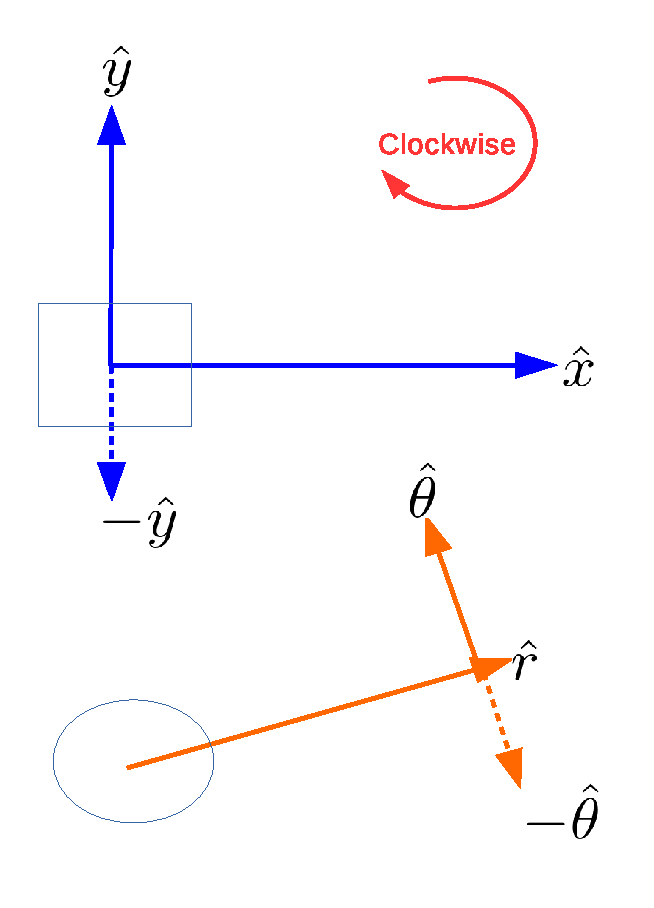
\includegraphics[scale=0.5]{images/c08-psisignconvention.eps}
}
\end{center}
\caption{Sign convention for stream function}
\label{psisignconvention}
\end{figure}


    Rectangular: 
    $$V_x = {\partial \psi \over \partial y} \, \& \, V_y = - {\partial \psi \over \partial x} $$
{\bf Convention}
Differentiation of $\psi$ in a direction gives velocity component $90^o$ clockwise from that direction.
    Cylindrical:
 $$ V_r = {1 \over r} {\partial \psi \over \partial \theta} \, \, \& \, \, V_\theta = - {\partial \psi \over \partial r} $$

{\bf Meaning of $\psi$}


\begin{figure}[h]
\begin{center}
\framebox{ 
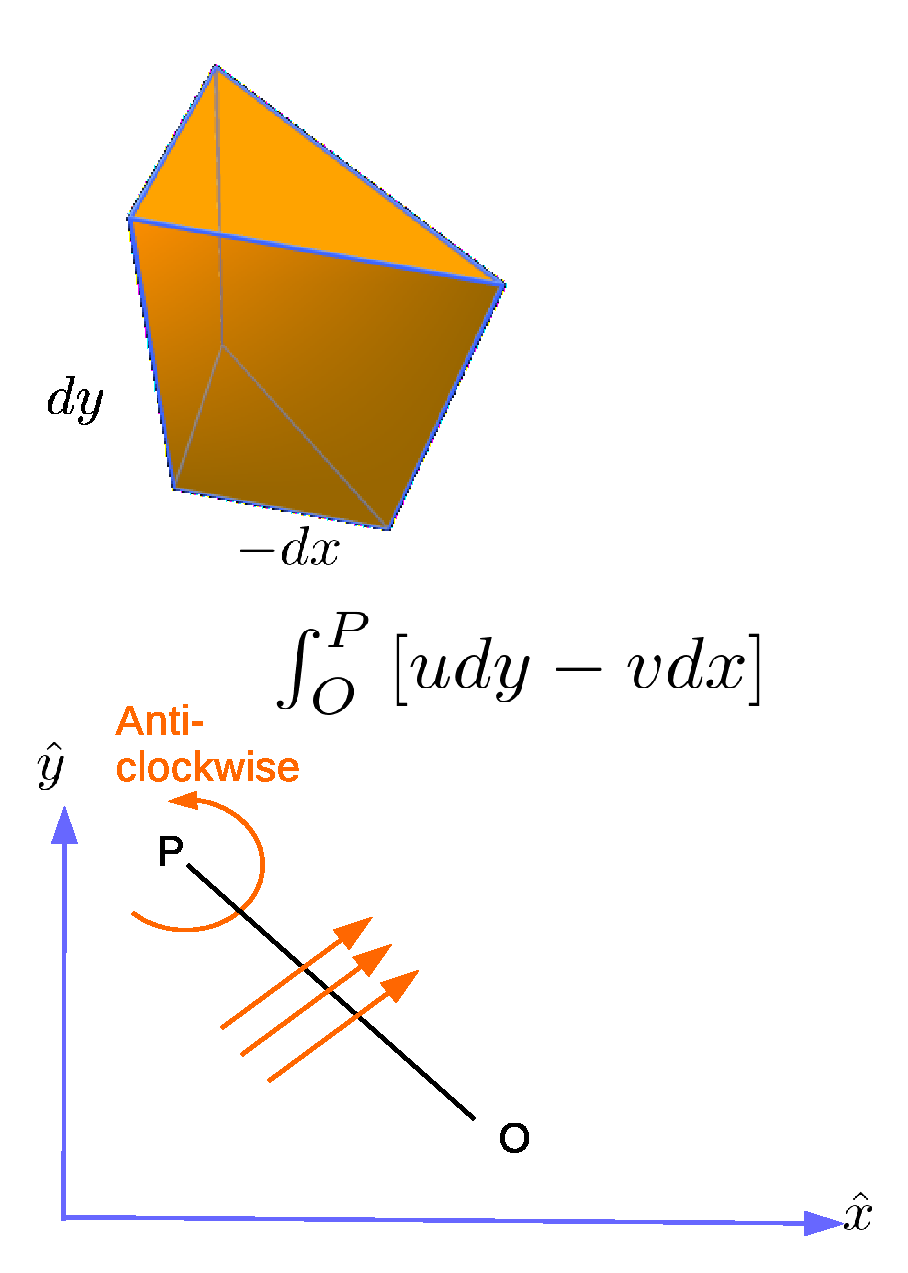
\includegraphics[scale=0.5]{images/c08-psiflowconvention.eps}
}
\end{center}
\caption{Convention for flow direction using contours of stream function}
\label{psiflowconvention}
\end{figure}

If the flow is two dimensional, with only $r$ and $\theta$ components, then we can introduce the stream function $\psi$ as 

\begin{equation}
u_r \equiv {1 \over r} {\partial \psi \over \partial \theta}
\end{equation}

\begin{equation}
u_\theta \equiv - {\partial \psi \over \partial r}
\end{equation}

such that the continuity equation 

\begin{equation}
{\partial \left(r u_r\right) \over \partial r} + {\partial u_\theta \over \partial \theta} = 0
\end{equation}

is satisfied by the fact that the order of differentiation of $\psi$ with respect to $r$ and $\theta$ does not matter.


{\bf Convention}
Flux of fluid volume across a line OP is taken positive when it is in the anti-clockwise sense about P.

Exact differential of $\psi$:
$$ d\psi = {\partial \psi \over \partial x} dx +  {\partial \psi \over \partial y} dy = -v dx + u dy $$
$$ \psi_P - \psi_O = \int_{O}^{P}{\left[u dy - v dx\right]}$$

$\psi$ is flux of fluid volume across a line OP.

% -----------------------------------------------------

{\bf Stream function $\psi\left(r,\theta\right)$}

Assume $V_z = 0$, no $z$-dependence

Continuity equation in 2D:
$$ {1 \over r} {\partial \over \partial r} \left( r V_r \right) + {1 \over r} {\partial V_\theta \over \partial \theta} = 0 $$

Define $\psi$ such that:
 $$ V_r = {1 \over r} {\partial \psi \over \partial \theta} \, \, \& \, \, V_\theta = - {\partial \psi \over \partial r} $$


% -----------------------------------------------------

{\bf Stream function $\psi\left(r,z\right)$}

Assume $V_\theta = 0$, no $\theta$-dependence

Continuity equation in 2D:
$$ {1 \over r} {\partial \over \partial r} \left( r V_r \right) + {\partial V_z \over \partial z} = 0 $$

Define $\psi$ such that:
 $$ V_r = {1 \over r} {\partial \psi \over \partial z} \, \, \& \, \, V_z = -{1 \over r} {\partial \psi \over \partial r} $$

% -----------------------------------------------------

{\bf Stream function $\psi\left(r,\theta\right)$}

Assume $V_\phi = 0$, no $\phi$-dependence

Continuity equation in 2D:
$$ {1 \over r^2} {\partial \over \partial r} \left( r^2 V_r \right) + {1 \over r \sin\theta} {\partial \over \partial \theta} \left( V_\theta \sin\theta \right) = 0 $$

Define $\psi$ such that:
 $$ V_r = {1 \over r^2 \sin\theta} {\partial \psi \over \partial \theta} \, \, \& \, \, V_\theta = - {1 \over r \sin\theta} {\partial \psi \over \partial r} $$


% -----------------------------------------------------------------------

% learning objective
\begin {lo3} [Fluid Flow]
Validate a velocity profile as irrotational
\end {lo3}

\section{Vorticity}

Vorticity is often represented using $\omega$.

{\bf Definition}
$$ \omega = \vec{\nabla} \times \vec{u}$$

{\bf Circulation} $\Gamma$ is line integral of tangential velocity component about a closed curve C fixed in the flow.
$$ \Gamma = \oint_{C}{\vec{u} \times \vec{dS}}$$

Stokes theorem in 2D:
$$ \Gamma = \oint_{C}{\vec{u} \times \vec{dS}} = \int_{A}{\vec{\nabla} \times \vec{u} dA} =  \int_{A}{\vec{\omega} \cdot \hat{n} dA} $$ 

In an {\bf irrotational} flow fluid elements do not undergo any rotation:
$$ \omega = 0 $$ 

% -----------------------------------------------------------------------

% learning objective
\begin {lo3} [Fluid Flow]
Apply definition of velocity potential to determine velocity components
\end {lo3}

\section{Velocity potential}

Velocity potential is often represented using $\Phi$.

Using the vector identity $\vec{\nabla} \times \vec{\nabla} \Phi = 0$ for any scalar function $\Phi$, one can propose a {\bf potential} to determine velocity fields of an {\bf irrotational flow}.

Flow is down the potential gradient. Let's define $\Phi$ such that:
$$ \vec{u} = -\vec{\nabla}\Phi $$
$$ u_1 = -{\partial \Phi \over \partial x_1} \, \, \& \, \, u_2 = -{\partial \Phi \over \partial x_2} $$


% -----------------------------------------------------------------------

{\bf Generating velocity potentials}

Continuity equation for incompressible fluids:
$$ \vec{\nabla} \cdot \vec{u} = - \vec{\nabla} \cdot \vec{\nabla}\Phi = 0 \implies  \nabla^2 \phi = 0 $$

Any scalar function that satisfies the Laplace's equation can be used as $\Phi$ to generate 2D velocity field.

Unlike stream function, velocity potentials can be used in 3D too.


% -----------------------------------------------------------------------

\section{Potential flow}

Potential flow in cylindrical coordinate system:

Define $\Phi$ such that:
$$ u_r = -{\partial \Phi \over \partial r} \, \, \& \, \, u_\theta = -{1 \over r}{\partial \Phi \over \partial \theta} $$

Continuity equation in 2D becomes:
$$ {\partial^2 \Phi \over \partial r^2} + {1 \over r}{\partial \Phi \over \partial r}+ {1 \over r^2} {\partial^2 \Phi \over \partial \theta^2} = -\nabla^2 \Phi = 0 $$

Any scalar function that satisfies the Laplace's equation can be used as $\Phi$ to generate 2D velocity field.

% -----------------------------------------------------------------------

{\bf Stream function and velocity potential}

\begin{enumerate}
\item Difference in values of contours of $\psi$ represent volume flow between them.
\item Velocity vector at any point is tangential to the contour of $\psi$ through the point
\item Contours of $\psi$ indicate the sense of flow.
\item Contours of $\Phi$ are normal to those of $\psi$.
\end{enumerate}


% -----------------------------------------------------------------------

% learning objective
\begin {lo3} [Fluid Flow]
Plot elementary planar flows
\end {lo3}

\section{Elementary planar flows}

\subsection{Uniform flow}

Stream function $\psi$:

$\psi = A y$ or $\psi = Ar \cos\theta$

Velocity Potential $\Phi$:

$\Phi = -A x$ or $\Phi = Ar \sin\theta$

Velocities:

$ u = A$, $v=0$

\begin{figure}[h]
\begin{center}
\framebox{ 
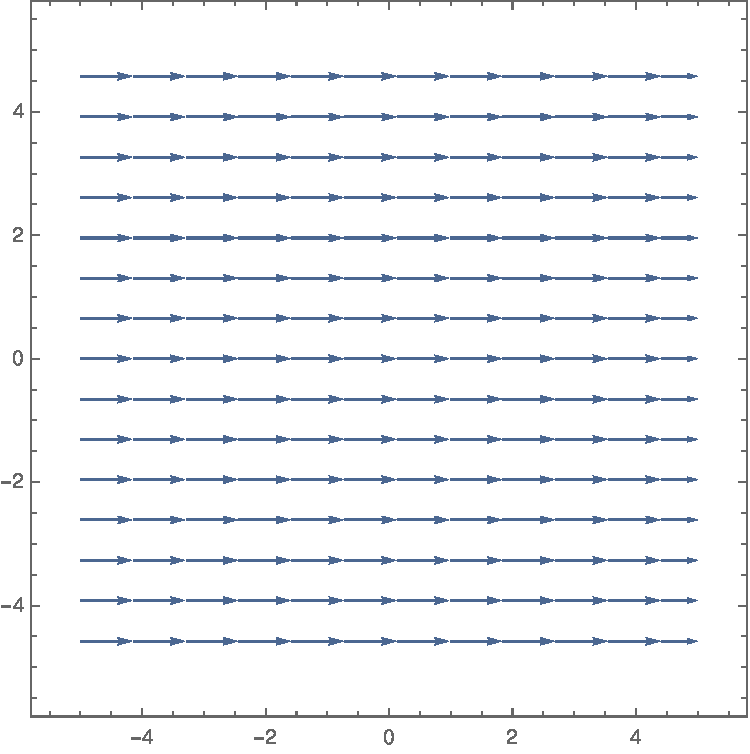
\includegraphics[scale=0.5]{images/c08-UniformFlow.ps}
}
\end{center}
\caption{Uniform flow using potential function}
\label{planaruniformflow}
\end{figure}



% -----------------------------------------------------------------------

\subsection{Stagnation flow}

Stream function $\psi$:

$$\psi = -2xy$$
Velocity Potential $\Phi$:
$$\Phi = x^2 - y^2$$
Velocities:

$ u = -2x$ \, $v = 2y$

\begin{figure}[h]
\begin{center}
\framebox{ 
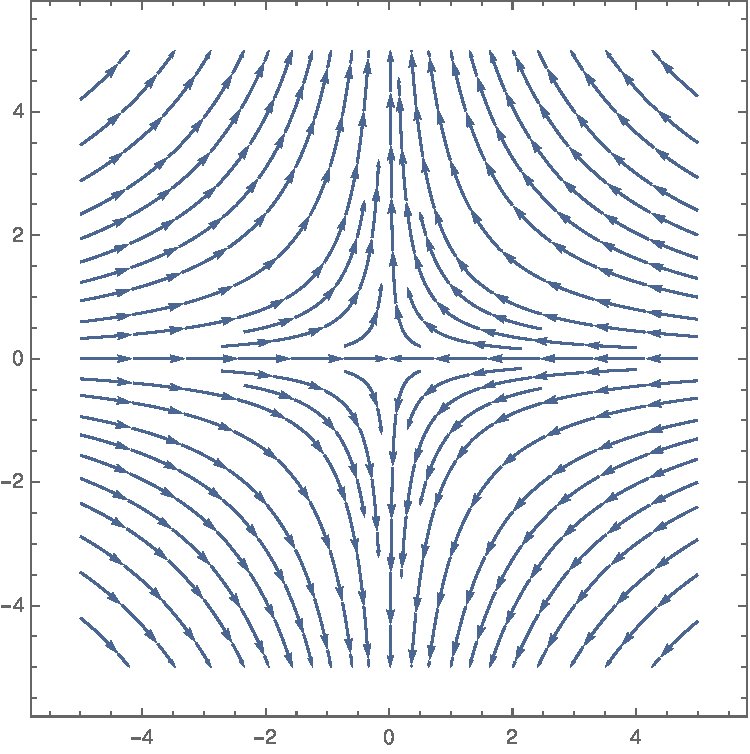
\includegraphics[scale=0.5]{images/c08-StagnationFlow.ps}
}
\end{center}
\caption{Stagnation flow using potential function}
\label{planarstagnationflow}
\end{figure}


% -----------------------------------------------------------------------

\subsection{Sink flow}

$Q$ is  volume flow rate per unit depth

Stream function $\psi$:

$\psi = {-Q \over 2\pi} \theta$

Velocity Potential $\Phi$:

$\Phi = {Q \over 2\pi} \ln r$

Velocities:

$u_r = {-Q \over 2 \pi r}$,  $u_\theta = 0$

\begin{figure}[h]
\begin{center}
\framebox{ 
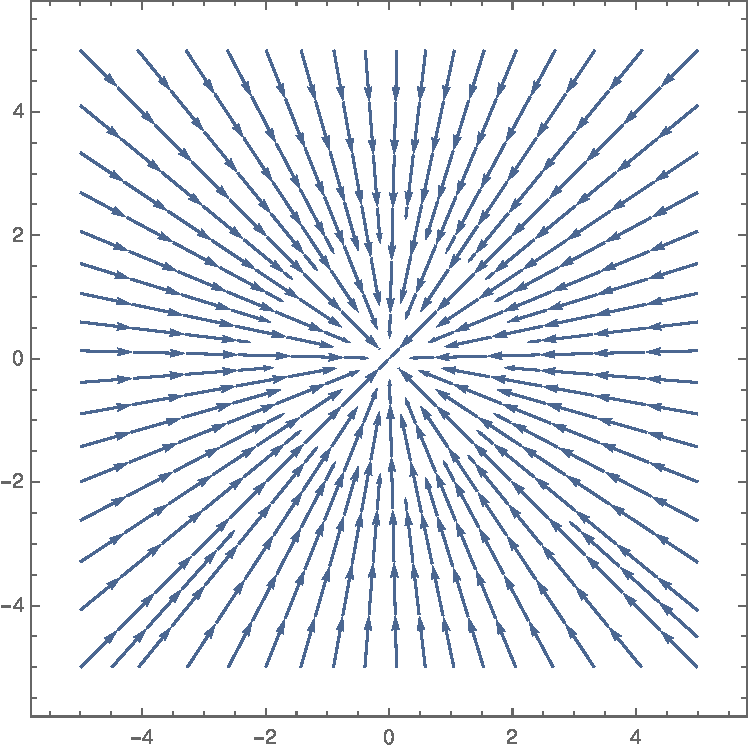
\includegraphics[scale=0.5]{images/c08-SinkFlow.ps}
}
\end{center}
\caption{Sink flow using potential function}
\label{planarsinkflow}
\end{figure}


% -----------------------------------------------------------------------
\subsection{Source flow}

$Q$ is  volume flow rate per unit depth

Stream function $\psi$:

$\psi = {Q \over 2\pi} \theta$

Velocity Potential $\Phi$:

$\Phi = {-Q \over 2\pi} \ln r$

Velocities:

$u_r = {Q \over 2\pi r}$,  $u_\theta = 0$

\begin{figure}[h]
\begin{center}
\framebox{ 
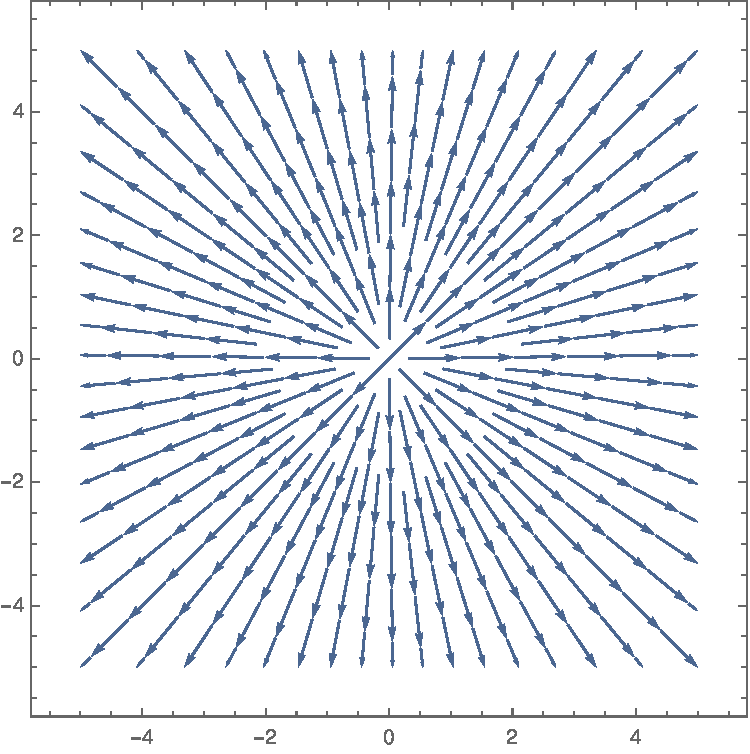
\includegraphics[scale=0.5]{images/c08-SourceFlow.ps}
}
\end{center}
\caption{Source flow using potential function}
\label{planarsourceflow}
\end{figure}

% -----------------------------------------------------------------------

\subsection{Doublet}

$A$ is strengh of doublet.

Stream function $\psi$:
$$\psi = {-A \sin\theta \over r}$$

Velocity Potential $\Phi$:
$$\Phi = {-A\cos\theta \over r}$$

Velocities:

$u_r = {-A \cos\theta \over r^2}$, $u_\theta = {-A \sin\theta \over r^2}$

\begin{figure}[h]
\begin{center}
\framebox{ 
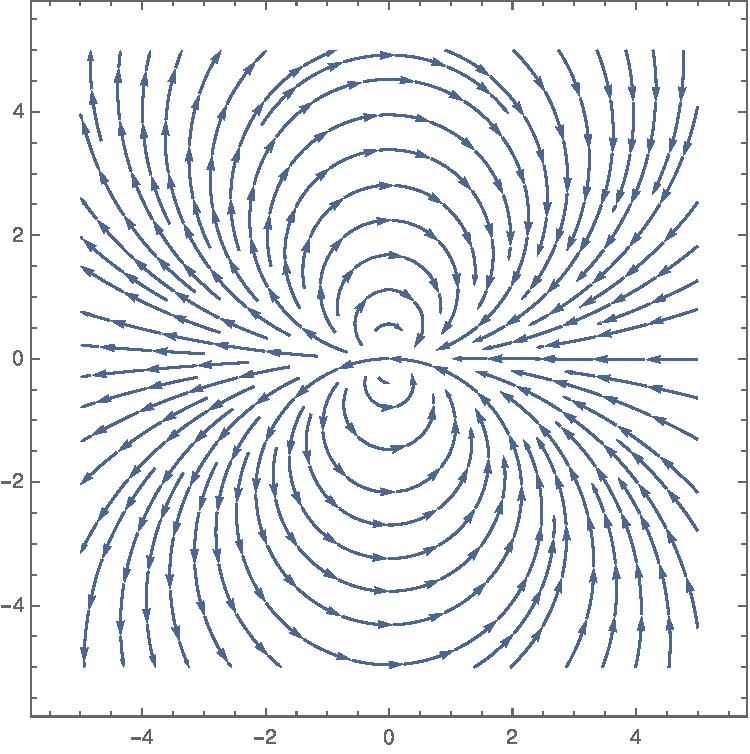
\includegraphics[scale=0.4]{images/c08-Doublet.ps}
}
\end{center}
\caption{Doublet flow using potential function}
\label{planardoubletflow}
\end{figure}


% -----------------------------------------------------------------------
\subsection{Vortex}

$A$ is strength of vortex

Stream function $\psi$:
$$\psi = {-A \over 2\pi} \ln r$$

Velocity Potential $\Phi$:

$$\Phi = {-A \over 2 \pi} \theta $$

Velocities:

$u_r =0$, $u_\theta={A \over 2 \pi r}$

\begin{figure}[h]
\begin{center}
\framebox{ 
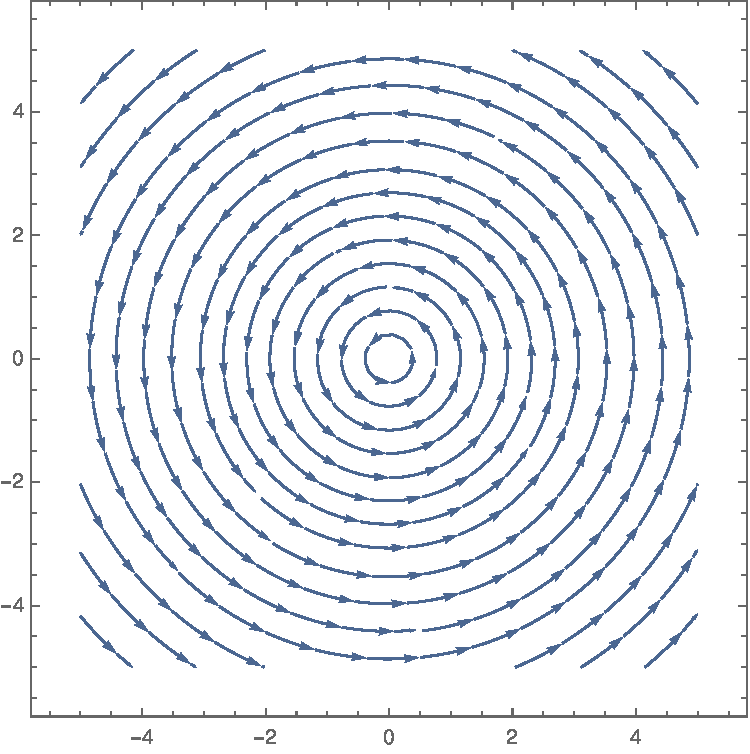
\includegraphics[scale=0.4]{images/c08-Vortex.ps}
}
\end{center}
\caption{Vortex flow using potential function}
\label{planarvortexflow}
\end{figure}


% -----------------------------------------------------------------------

\subsection{Combinations of elementary planar flows}

Source flow + Uniform flow $\rightarrow$ Flow past a half-body

\begin{figure}[h]
\begin{center}
\framebox{ 
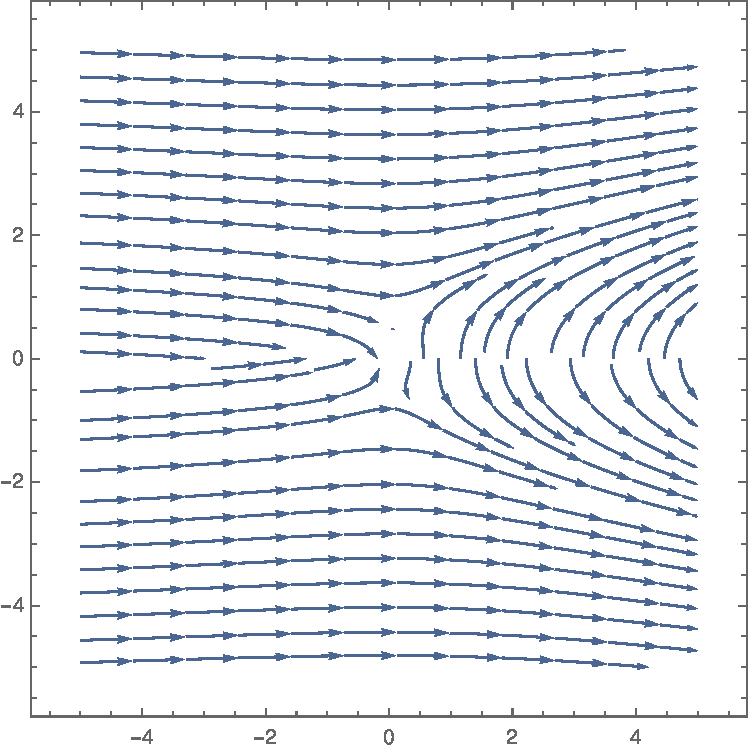
\includegraphics[scale=0.4]{images/c08-SourceUniform.ps}
}
\end{center}
\caption{Source + Uniform flow using potential function}
\label{planarsourceuniformflow}
\end{figure}


Source or Sink flow + Vortex $\rightarrow$ Spiral flow
\begin{figure}[h]
\begin{center}
\framebox{ 
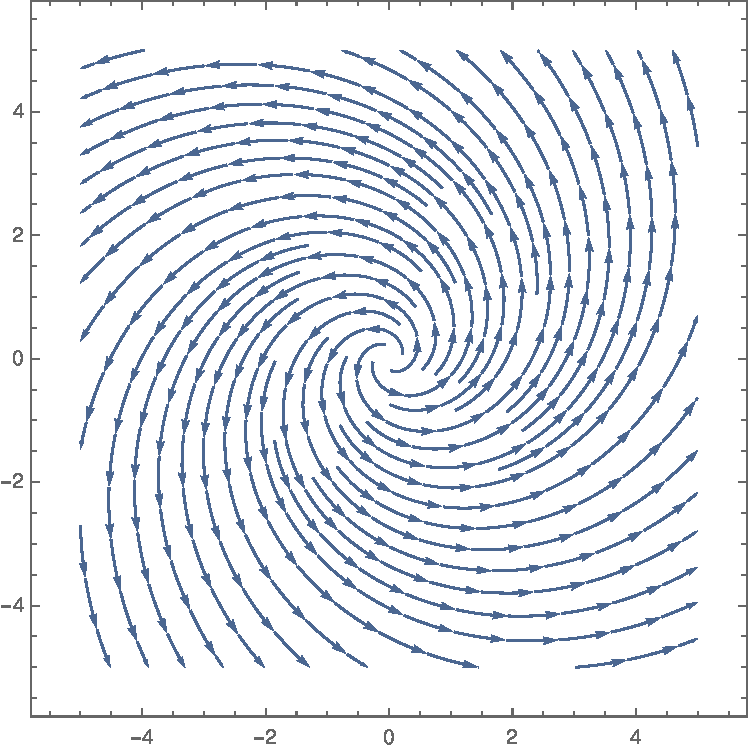
\includegraphics[scale=0.4]{images/c08-SourceVortex.ps}
}
\end{center}
\caption{Source + Vortex flow using potential function}
\label{planarsourcevortexflow}
\end{figure}


% -----------------------------------------------------------------------

{\bf Combinations of elementary planar flows}

Doublet + Uniform flow $\rightarrow$ Flow past a cylinder

\begin{figure}[h]
\begin{center}
\framebox{ 
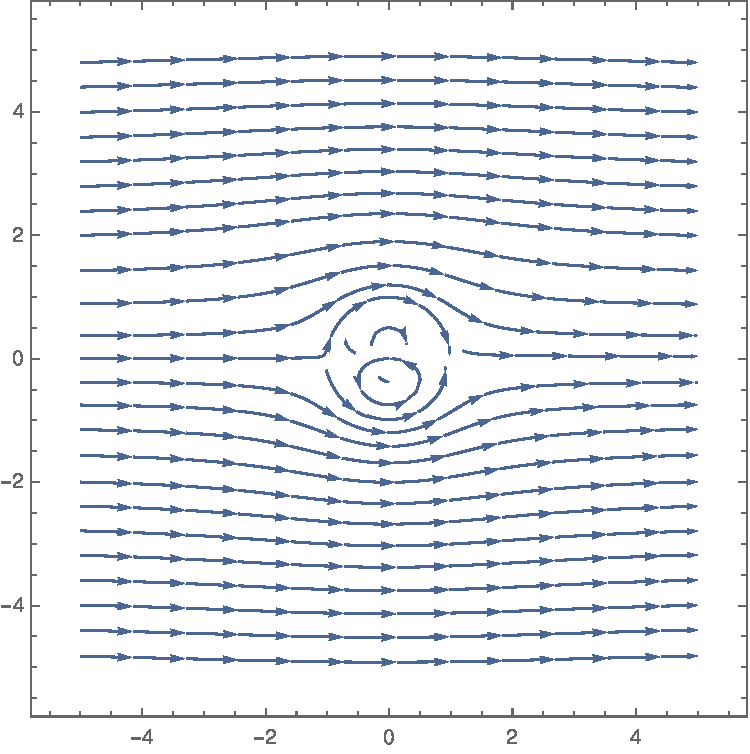
\includegraphics[scale=0.4]{images/c08-DoubletUniform.ps}
}
\end{center}
\caption{Doublet + Uniform flow using potential function}
\label{planardoubletuniformflow}
\end{figure}


Doublet +Vortex + Uniform flow $\rightarrow$ Flow past a cylinder with circulation

\begin{figure}[h]
\begin{center}
\framebox{ 
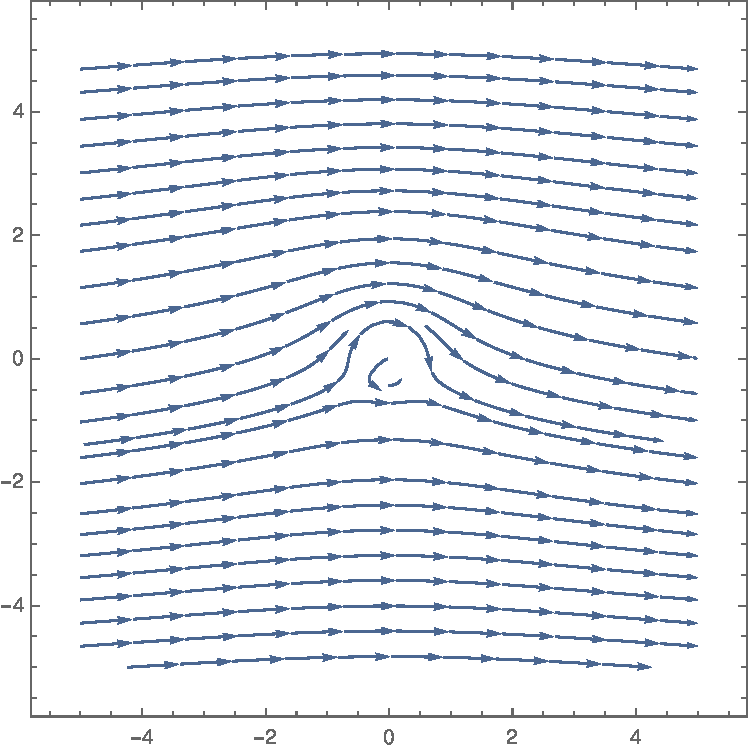
\includegraphics[scale=0.4]{images/c08-DoubletVortexUniform.ps}
}
\end{center}
\caption{Doublet + Vortex + Uniform flow using potential function}
\label{planardoubletvortexuniformflow}
\end{figure}


% -----------------------------------------------------------------------

%{\bf Applications in materials processing}
%Tapping liquid metal from a ladle
%\includegraphics[width=5in]{images/TundishMold.png}\\
%\includegraphics[width=5in]{images/concast.png}\\
%{\small ref: \tt www.wikipedia.com}

%Gas flow through nozzles
%\includegraphics[width=5in]{images/GTAW.jpg}\\
%{\small ref: \tt www.wikipedia.com}

% -----------------------------------------------------------------------

\section{Summary}

\begin{enumerate}
\item Stream function relations
\item Vorticity relations
\item Condition for irrotational flow
\end{enumerate}

% -----------------------------------------------------------------------

\section{Further study}

\begin{enumerate}
\item The velocity field near the core of a tornado can be approximated as following.
$$ \vec{u} = -{q \over 2 \pi r} \hat{e}_r + {K \over 2 \pi r} \hat{e}_\theta $$
Is this an irrotational flow field? Obtain the stream function for this flow. \\ Ans: $\psi = -\left( q\theta+K\ln r \right)/2\pi$.

\item An incompressible flow field is defined using stream function as follows. $$ \psi = A\left(x^2-y^2\right)$$
Determine the velocity components of this flow field. Also, check if this flow field is irrotation and if so, determine the velocity potential $\phi$ for this flow.

\item Using the definitions of $\psi$ and $\phi$ and the continuity equation for a 2D flow field, show that any scalar function that satisfies the Laplace's equation can represent a 2D, irrotational, incompressible flow field.

\item Volume flow rate across two streamlines is given by $Q=\int{u dl}$ where $l$ is the distance across the two streamlines. Convince yourself that the volume flow rate Q between two streamlines $\psi_1$ and $\psi_2$ is $\psi_2-\psi_1$. \\ Hint: Write the exact differential for $\psi$ and evaluate the flow rate between two streamlines keeping either $x$ or $y$ constant.

\item Convince yourself that the constant $\psi$ line at any point is negative reciprocal to the slope of $\phi$ at that point.\\ Hint: Use exact differential of $\psi$ and $\phi$ and write $ \left( {\partial y \over \partial x} \right)_\psi$ etc.,

\item A flow field where the streamlines are concentric circles is called a vortex. What kind of functional form can you think of for the velocity components in a vortex?
 
\item During welding, argon gas jet is used to protect the liquid melt pool. The gas flows down the cylindrical tube kept at a small height from the plate being welded. Draw schematically the flow field for this situation and design a possible functional form for the velocity components in different regions of this problem.\\ Hint: There are regions where the flow is unidirectional and where the flow is radially outward (source flow). 

\end{enumerate}

% -----------------------------------------------------------------------

\chapter{Navier-Stokes Equations - Part 1}
\label{ch:nsderive1}

\section{Learning objectives}

At the end of this lesson, a student should be able to
\begin{enumerate}
\item perform algebraic analysis using subscript notation
\item identify the terms and their role in the Navier-Stokes equations
\item recall Navier-Stokes equations in rectangular coordinate system
\item derive and recall definition of Reynold's number
\item analyse the dominant terms of Navier-Stokes equations for small and large values of Reynold's number
\end{enumerate}

\section{Concept map}

% learning objective
\begin{lo2}[Fluid Flow]
  List the concepts behind Navier-Stokes equations
\end{lo2}

The starting point for momentum balance equation is Newton's second law of motion applied to a moving volume element in a fluid.


The strategy to derive Navier-Stokes equation \index{Navier-Stokes equation} is illustrated in the concept map below.

\begin{figure}[h]
 \centering
 \includegraphics[width=6 in]{images/c09-NavierStokesFlowChart2.eps}
 % ctrans.eps: 46x0 pixel, 300dpi, 0.39x0.00 cm, bb=0 35 595 420
 \caption{Concept map of derivation of Navier-Stokes equation}
 \label{nsconceptmap}
\end{figure}


\section{Forces}

{\bf Long range forces} decrease slowly with increase in distance between the interacting elements. These are called body forces or volume forces. Examples such as gravity (due to density $\rho$ gradients), electromagnetic (in metals carrying electric currents) and fictitious (centrifugal or coriolis) act on the whole of the fluid element and are usually proportional to the size of the volume element ($\delta V$). They can be represented as:

$$ F_i(x_i,t) \rho \delta V $$

Eg. gravity pointing vertically downwards :

$$ F_i = g \hat{x}_2 $$

{\bf Short range forces} decrease rapidly with increase in distance between the interacting elements and are of molecular origin. Examples such as forces applied on surfaces (normal and shear), Marangoni forces (due to surface tension gradients) act on a thin layer of the fluid and are called surface forces. Local short range forces exerted by the fluid on different surface elements ($\delta A$) can be represented as:

$$ \sigma(x_i, n_j, t) \delta A $$

where, $n_j$ is the unit normal to the surface element $\delta A$. $\sigma$ is called the local {\bf stress}.

\section{Equation of motion}

% learning objective
\begin {lo3} [Fluid Flow]
Derive equation of motion
\end {lo3}

Consider a moving fluid element of volume $dV$ and area $dS$ on a surface with normal $n_i$. Using the material derivative $\frac{D}{Dt}$ introduced earlier, the rate of change of momentum of a small fluid element of volume $dv$ is given by:

$$ \frac{D}{Dt} \int_{V}{\rho u_i dV} $$

Using the Reynold's transport theorem \index{Reynolds transport theorem} [\ref{rtt}] and the continuity equation, one can bring the material derivative inside the integral as illustrated in section [\ref{ktt}]. 

$$ \frac{D}{Dt} \int_{V}{\rho u_i dV} =  \int_{V}{\rho \frac{Du_i}{Dt} dV} $$

The total force that acts on $dV$ is the sum of body forces and surface forces:

$$ \int_{V}{F_i\rho dV} + \int_{S}{\sigma_{ij}n_jdS} $$

Using Gauss divergence theorem, \index{Gauss Divergence theorem}

\begin{equation}
\int_{S}{\sigma_{ij}n_jdS} = \int_{V}{\frac{\partial \sigma_{ij}}{\partial x_j}dV}
\end{equation} 

From Newton's second law, the rate of change of momentum is equal to the total force acting on the element. Hence,

\begin{equation}
\int_{V}{\frac{Du_i}{Dt}\rho dV}  =  \int_{V}{F_i\rho dV} + \int_{V}{\frac{\partial \sigma_{ij}}{\partial x_j}dV}
\end{equation} 

Since the three integrands are being summed over the same volume element, it will be applicable at {\em any} location in the fluid if the equation applies to the integrands themselves:

\begin{equation}
\label{eqmotion}
\boxed{\frac{Du_i}{Dt}\rho =  F_i\rho + \frac{\partial \sigma_{ij}}{\partial x_j}}
\end{equation} 

We now need to express $\sigma_{ij}$ in a way that can minimise the number of unknown parameters in the above equation of motion.

\section{Stress tensor}

Section \ref{cauchy} stating the Cauchy's stress principle and section \ref{stresstensor} prove that stress is a tensor. We can also use conservation of angular momentum to show that the stress tensor is symmetric as described in section \ref{symstress}. Hence it can be expressed as 

\begin{equation}
\sigma_{ij} = \left(
\begin{array}{lll}
\sigma_{11} & \sigma_{12} & \sigma_{13} \\ 
\sigma_{12} & \sigma_{22} & \sigma_{23} \\ 
\sigma_{13} & \sigma_{23} & \sigma_{33} \\ 
\end{array}
\right)
\end{equation} 

Since it is always possible to find a co-ordinate system such that the matrix containing the elements of a symmetric tensor is diagonal, we can write $\sigma_{ij}$ as the follows.


\begin{equation}
\sigma_{ij} = \left(
\begin{array}{lll}
\sigma_{11} & 0 & 0 \\ 
0 & \sigma_{22} & 0 \\ 
0 & 0 & \sigma_{33} \\ 
\end{array}
\right)
\end{equation} 

or 

\begin{equation}
\sigma_{ij} = \left(
\begin{array}{lll}
\frac{1}{3}\sigma_{kk} & 0 & 0 \\ 
0 & \frac{1}{3}\sigma_{kk} & 0 \\ 
0 & 0 & \frac{1}{3}\sigma_{kk} \\ 
\end{array}
\right) + \left(
\begin{array}{lll}
\sigma_{11}-\frac{1}{3}\sigma_{kk} & 0 & 0 \\ 
0 & \sigma_{22}-\frac{1}{3}\sigma_{kk} & 0 \\ 
0 & 0 & \sigma_{33}-\frac{1}{3}\sigma_{kk} \\ 
\end{array}
\right) 
\end{equation} 

where

\begin{equation}
\sigma_{kk}=\sigma_{11} + \sigma_{22} + \sigma_{33}
\end{equation} 

\begin{equation}
\sigma_{ij} = \frac{1}{3}\sigma_{kk}\delta_{ij} +  d_{ij}
\end{equation} 

We define static pressure of the fluid with the convention that positive pressure is that which acts to compress a fluid element,

\begin{equation}
p = -\frac{1}{3}\sigma_{kk}
\end{equation} 

so that 

\begin{equation}
\label{sigmaij}
\sigma_{ij} = -p\delta_{ij} +  d_{ij}
\end{equation} 

\index{Deviatoric stress}
$d_{ij}$ is called the {\em deviatoric} part of the tensor and leads only to volume conserving deformation of the fluid elements ie., flow of the fluid. Static pressure, on the other hand, leads to a shape-conserving change in the volume element. It is easy to note that 

\begin{equation}
d_{kk} = 0
\end{equation} 

We have separated the stress into two terms:
\begin{itemize}
\item 
{\em pressure} \index{Pressure} term ($-p\delta_{ij}$) that tends to change the volume of a fluid element 
\item 
{\em deviatoric stress} term ($d_{ij}$) that tends to change the shape of a fluid element while keeping the volume constant
\end{itemize}

By analysing all modes of change of shape of a fluid element, we can relate the deviatoric stress with the terms that quantify the shape changes of a fluid element. For non-zero velocity field, because the fluid element translates as time progresses, we will notice that rate of change of shape is more appropriate to analyse a fluid element.

\section{Strain rate tensor}

\index{Strain rate tensor}

The meaning of velocity gradient or a strain rate term $\frac{\partial u_i}{\partial x_j}$ is given in section \ref{strainratemeaning}. Proof that velocity gradient is a tensor of order two is given in section \ref{strainratetensor}. Strain rate or velocity gradient is represented as below and can be shown to be a second order tensor and thus expressible as a sum of symmetric and anti-symmetric tensors. 

\begin{equation}
\frac{\partial u_i}{\partial x_j} = e_{ij} + \Omega_{ij} 
\end{equation} 

\begin{equation}
e_{ij} = \frac{1}{2} \left( \frac{\partial u_i}{\partial x_j} + \frac{\partial u_j}{\partial x_i} \right) 
\end{equation} 

\begin{equation}
\Omega_{ij} = \frac{1}{2} \left( \frac{\partial u_i}{\partial x_j} - \frac{\partial u_j}{\partial x_i} \right) 
\end{equation} 

Define $\omega$ as 

\begin{equation}
\vec{\omega} = \vnabla \times \vec{u} 
\end{equation} 

or

\begin{equation}
\omega_i = \epsilon_{ijk}u_{j,k} = \epsilon_{ijk} \frac{\partial u_j}{\partial x_k} 
\end{equation} 

so that,

\begin{equation}
\Omega_{ij} = -\frac{1}{2}\epsilon_{ijk}\omega_k
\end{equation} 


\section{Relation between stress and strain-rate}

A relation between the deviatoric stress and strain-rate (velocity gradient) is necessary to proceed further to be able to use the equation of motion to solve for the velocity $u_i$. We have to adopt a {\em phenomenological} approach. 

\begin{list}{}{}
\item By definition, $d_{ij}$ is the deviatoric stress which implies that it is zero for a stationary fluid.
\item The velocities and thus the velocity gradients $\frac{\partial u_i}{\partial x_j}$ are zero for a stationary fluid.
\item The deviatoric stress represents the frictional interaction between different layers of the fluid and is assumed to be dependent only on the instantaneous and local distribution of the velocities. 
\end{list} 

From the above observations, we may {\em assume} that the deviatoric stress and the strain-rate are directly and {\em linearly} related to each other. Since both the quantities are tensors of order two, the entity that connects them both must be a tensor of order four.

\begin{equation}
d_{ij} = A_{ijkl} \frac{\partial u_k}{\partial x_l}
\end{equation} 

Since the above equation connects an effect with a cause, it is a {\em constitutive relation}
and the entity $A_{ijkl}$ is a physical parameter. The material in concern is a fluid in which a directionality can safely be assumed to be absent ie., 

\begin{center}
{\em fluids are isotropic}
\end{center}

 Hence, $A_{ijkl}$ must possess the same properties as that of an isotropic tensor of order four. From the properties of tensors, we know that the general form of an isotropic tensor of order four [\ref{isotensorfour}] is 

\begin{equation}
A_{ijkl} = \mu_1 \delta_{ij}\delta_{kl} + \mu_2 \delta_{il}\delta_{kj} + \mu_3 \delta_{ik}\delta_{jl}
\end{equation} 

Since deviatoric stress $d_{ij}$ is symmetric, interchanging the subscripts $i$ and $j$ should keep the quantity identical. In the above equation, this applies also to the R.H.S. ie.,

\begin{equation}
A_{ijkl} = A_{jikl} \Rightarrow \mu_2 = \mu_3
\end{equation} 

\begin{equation}
A_{ijkl} = \mu_1 \delta_{ij}\delta_{kl} + \mu_2 \left( \delta_{il}\delta_{kj} + \delta_{ik}\delta_{jl} \right)
\end{equation} 

$A_{ijkl}$ is now symmetrical in $k$ and $l$ also.

Expanding the above equation,

\begin{equation}
d_{ij} = A_{ijkl} \left( e_{kl} + \Omega_{kl} \right)
\end{equation} 

Since $A_{ijkl}$ is now symmetrical in $k$ and $l$, when it is multiplied by an entity that is anti-symmetric about $k$ and $l$ and the terms are summed over $k$ and $l$ they vanish. Thus, the $\Omega_{kl}$ term drops out.

\begin{equation}
d_{ij} = \left( \mu_1 \delta_{ij}\delta_{kl} + \mu_2 \left( \delta_{il}\delta_{kj} + \delta_{ik}\delta_{jl} \right) \right) e_{kl}
\end{equation} 

\begin{equation}
d_{ij} = \mu_1 \delta_{ij}\delta_{kl}e_{kl} + \mu_2 \left( \delta_{il}\delta_{kj}e_{kl} + \delta_{ik}\delta_{jl}e_{kl} \right)
\end{equation} 

\index{Compressibility}
\index{Rate of dilation}
\index{Rate of expansion}

We have already (\ref{rdiln}) defined {\em compressibility} or {rate of dilation} or rate of expansion as

\begin{equation}
e_{kk} = \frac{\partial u_1}{\partial x_1} + \frac{\partial u_2}{\partial x_2} + \frac{\partial u_3}{\partial x_3} = \Delta 
\end{equation} 

For the first term, we use the contraction theorem [section \ref{contraction}] to get

\begin{equation}
d_{ij} = \mu_1 \delta_{ij}\Delta + 2 \mu_2 e_{ij}
\end{equation} 

Recalling that $d_{ii}=0$,

\begin{equation}
d_{ii} = \mu_1 3 \Delta + 2 \mu_2 \Delta = (3 \mu_1 + 2 \mu_2) \Delta = 0
\end{equation} 

We would like the above equation to be true also for incompressible fluids ie., also when $\Delta \ne 0$. It can be true only when the term in parantheses vanishes.

\index{Stokes assumption}

{\em Stokes' Assumption}: For monoatomic fluids since there is no conversion of translational energy into vibrationary / rotationary energies, {\em bulk viscosity} can be assumed to be zero:

$$(3 \mu_1 + 2 \mu_2)=0$$ 

or

\begin{equation}
\mu_1 = -\frac{2}{3} \mu_2 
\end{equation} 

Watch out for fluids for which Stokes' assumption is not valid. 

Calling the one constant parameter as $\mu$, the equation becomes

\begin{equation}
d_{ij} = - \frac{2}{3} \mu \delta_{ij} \Delta + 2 \mu e_{ij}
\end{equation} 

\begin{equation}
\label{dij}
d_{ij} = 2 \mu \left( e_{ij} - \frac{1}{3} \Delta \delta_{ij} \right)
\end{equation} 


Now that we have an expression for $d_{ij}$ in terms of velocity gradients, we can substitute the same in the equation of motion.

\section{Navier-Stokes equations}

\index{Navier-Stokes equation}

Combining equation of motion (\ref{eqmotion}) and the expressions for stress tensor (\ref{sigmaij} and \ref{dij}), we get,

\begin{equation}
\rho \frac{Du_i}{Dt} = \rho F_i + \frac{\partial}{\partial x_j} \left[ -p\delta_{ij}+ 2 \mu \left( e_{ij} - \frac{1}{3} \Delta \delta_{ij}\right)\right]
\end{equation} 

Expanding the term $e_{ij}$ and using the kronecker delta to contract subscripts, we get:

\begin{equation}
\rho \frac{Du_i}{Dt} = \rho F_i -  \frac{\partial p}{\partial x_i} +  
\frac{\partial}{\partial x_j} \left( \mu \frac{\partial u_i}{\partial x_j} \right) + 
\frac{\partial}{\partial x_j} \left( \mu \frac{\partial u_j}{\partial x_i} \right) + 
\frac{\partial}{\partial x_i} \left( -\frac{2}{3} \mu \Delta \right) 
\end{equation} 

Since the order of differentiation should not matter and if $\mu$ is not a function of location,
\begin{equation}
\rho \frac{Du_i}{Dt} = \rho F_i -  \frac{\partial p}{\partial x_i} +  
\frac{\partial}{\partial x_j} \left( \mu \frac{\partial u_i}{\partial x_j} \right) + 
\frac{\partial}{\partial x_i} \left( \mu \frac{\partial u_j}{\partial x_j} \right) + 
\frac{\partial}{\partial x_i} \left( -\frac{2}{3} \mu \Delta \right) 
\end{equation} 

\begin{equation}
\rho \frac{Du_i}{Dt} = \rho F_i -  \frac{\partial p}{\partial x_i} +  
\frac{\partial}{\partial x_j} \left( \mu \frac{\partial u_i}{\partial x_j} \right) + 
\frac{\partial}{\partial x_i} \left( \mu \Delta \right) + 
\frac{\partial}{\partial x_i} \left( -\frac{2}{3} \mu \Delta \right) 
\end{equation} 


\begin{equation}
\label{ns0}
\boxed{
\rho \frac{Du_i}{Dt} = \rho F_i -  \frac{\partial p}{\partial x_i} +  
\frac{\partial}{\partial x_j} \left( \mu \frac{\partial u_i}{\partial x_j} \right) + 
\frac{1}{3}\frac{\partial}{\partial x_i} \left( \mu \Delta \right) 
}
\end{equation} 

The above set of three equations (for $i=1,2,3$) corresponding to the three components of the velocity of the fluid ($u_1$, $u_2$ and $u_3$) is called {\bf Navier-Stokes equations}.

% which are also given below in expanded form for cartesian co-ordinate system:

%\begin{align}
%\label{ns1}
%\rho \left[ 
%\frac{\partial u_1}{\partial t} + u_1\frac{\partial u_1}{\partial x_1} + u_2\frac{\partial u_1}{\partial x_2} + u_3\frac{\partial %u_1}{\partial x_3} 
%\right] & = \rho F_1 -  \frac{\partial p}{\partial x_1} \nonumber \\
%& + \frac{\partial}{\partial x_1} \left(\mu \frac{\partial u_1}{\partial x_1}\right) + \frac{\partial}{\partial x_2} \left( \mu %\frac{\partial u_1}{\partial x_2} \right) + \frac{\partial}{\partial x_3} \left( \mu \frac{\partial u_1}{\partial x_3} \right) \nonumber \\
%& + \frac{1}{3} \frac{\partial}{\partial x_1} \left[ \mu \left( \frac{\partial u_1}{\partial x_1} + \frac{\partial u_2}{\partial x_2} + %\frac{\partial u_3}{\partial x_3} \right)\right]
%\end{align} 

%\begin{align}
%\label{ns2}
%\rho \left[ 
%\frac{\partial u_2}{\partial t} + u_1\frac{\partial u_2}{\partial x_1} + u_2\frac{\partial u_2}{\partial x_2} + u_3\frac{\partial %u_2}{\partial x_3} 
%\right] & = \rho F_2 -  \frac{\partial p}{\partial x_2} \nonumber \\
%& + \frac{\partial}{\partial x_1} \left(\mu \frac{\partial u_2}{\partial x_1}\right) + \frac{\partial}{\partial x_2} \left( \mu %\frac{\partial u_2}{\partial x_2} \right) + \frac{\partial}{\partial x_3} \left( \mu \frac{\partial u_2}{\partial x_3} \right) \nonumber \\
%& + \frac{1}{3} \frac{\partial}{\partial x_2} \left[ \mu \left( \frac{\partial u_1}{\partial x_1} + \frac{\partial u_2}{\partial x_2} + %\frac{\partial u_3}{\partial x_3} \right)\right]
%\end{align} 

%\begin{align}
%\label{ns3}
%\rho \left[ 
%\frac{\partial u_3}{\partial t} + u_1\frac{\partial u_3}{\partial x_1} + u_2\frac{\partial u_3}{\partial x_2} + u_3\frac{\partial %u_3}{\partial x_3} 
%\right] & = \rho F_3 -  \frac{\partial p}{\partial x_3} \nonumber \\
%& + \frac{\partial}{\partial x_1} \left(\mu \frac{\partial u_3}{\partial x_1}\right) + \frac{\partial}{\partial x_2} \left( \mu %\frac{\partial u_3}{\partial x_2} \right) + \frac{\partial}{\partial x_3} \left( \mu \frac{\partial u_3}{\partial x_3} \right) \nonumber \\
%& + \frac{1}{3} \frac{\partial}{\partial x_3} \left[ \mu \left( \frac{\partial u_1}{\partial x_1} + \frac{\partial u_2}{\partial x_2} + %\frac{\partial u_3}{\partial x_3} \right)\right]
%\end{align} 

%Equations \ref{ns1}, \ref{ns2} and \ref{ns3} are the Navier-Stokes equations in cartesian co-ordinate system in complete form applicable for both compressible as well as incompressible Newtonian fluids. 

If the fluid being considered is incompressible, we can set the last term to zero and obtain the N-S equation with variable property.

A further simplification can be done starting from equation \ref{ns0} as follows. Most of the fluids under normal flow conditions are {\em incompressible} ie., $\Delta=0$. The Navier-Stokes equations for {\em incompressible} fluid flow with {\em constant viscosity} are obtained by taking $\mu$ out of the derivative and setting $\Delta=0$ in the equation~\ref{ns0}.

\begin{equation*}
\rho \frac{Du_i}{Dt} = \rho F_i -  \frac{\partial p}{\partial x_i} +  
\mu \frac{\partial^2 u_i}{\partial x_j^2} + \mu \left(\frac{\partial^2 u_j}{\partial x_j \partial x_i} \right) 
\end{equation*} 

\begin{equation*}
\rho \frac{Du_i}{Dt} = \rho F_i -  \frac{\partial p}{\partial x_i} +  
\mu \frac{\partial^2 u_i}{\partial x_j^2} + \mu \frac{\partial}{\partial x_i} \left(\frac{\partial u_j}{\partial x_j} \right) 
\end{equation*} 

\begin{equation*}
\rho \frac{Du_i}{Dt} = \rho F_i -  \frac{\partial p}{\partial x_i} +  
\mu \frac{\partial^2 u_i}{\partial x_j^2} + \mu \frac{\partial}{\partial x_i} \left(\Delta \right) 
\end{equation*} 

\begin{equation}
\label{nsa}
\rho \frac{Du_i}{Dt} = \rho F_i -  \frac{\partial p}{\partial x_i} +  
\mu \frac{\partial^2 u_i}{\partial x_j^2} 
\end{equation} 

Expanding the material derivative $\frac{D}{Dt}$ and writing in vector notation:

\begin{eqnarray}
\label{nsan}
\frac{\partial u_1}{\partial t} + (\vec{u}\cdot\vnabla)u_1 = F_1 -  \frac{1}{\rho} \frac{\partial p}{\partial x_1} +  \frac{\mu}{\rho} \nabla^2 u_1 
\nonumber \\
\frac{\partial u_2}{\partial t} + (\vec{u}\cdot\vnabla)u_2 = F_2 -  \frac{1}{\rho} \frac{\partial p}{\partial x_2} +  \frac{\mu}{\rho} \nabla^2 u_2 
\nonumber \\
\frac{\partial u_3}{\partial t} + (\vec{u}\cdot\vnabla)u_3 = F_3 -  \frac{1}{\rho} \frac{\partial p}{\partial x_3} +  \frac{\mu}{\rho} \nabla^2 u_3 
\end{eqnarray} 

These can be expanded to give the N-S equations for incompressible fluids of constant property using the definition of kinematic viscosity as follows:
$$\nu = \frac{\mu}{\rho}$$

\begin{equation}
\label{nsa1}
\boxed{
\frac{\partial u_1}{\partial t} + u_1\frac{\partial u_1}{\partial x_1} + u_2\frac{\partial u_1}{\partial x_2} + u_3\frac{\partial u_1}{\partial x_3} = F_1 -  \frac{1}{\rho}\frac{\partial p}{\partial x_1} + \nu \left( \frac{\partial^2 u_1}{\partial x_1^2} + \frac{\partial^2 u_1}{\partial x_2^2} + \frac{\partial^2 u_1}{\partial x_3^2} \right)
}
\end{equation} 

\begin{equation}
\label{nsa2}
\boxed{
\frac{\partial u_2}{\partial t} + u_1\frac{\partial u_2}{\partial x_1} + u_2\frac{\partial u_2}{\partial x_2} + u_3\frac{\partial u_2}{\partial x_3} = F_2 -  \frac{1}{\rho}\frac{\partial p}{\partial x_2} + \nu \left( \frac{\partial^2 u_2}{\partial x_1^2} + \frac{\partial^2 u_2}{\partial x_2^2} + \frac{\partial^2 u_2}{\partial x_3^2} \right)
}
\end{equation} 

\begin{equation}
\label{nsa3}
\boxed{
\frac{\partial u_3}{\partial t} + u_1\frac{\partial u_3}{\partial x_1} + u_2\frac{\partial u_3}{\partial x_2} + u_3\frac{\partial u_3}{\partial x_3} = F_3 -  \frac{1}{\rho}\frac{\partial p}{\partial x_3} + \nu \left( \frac{\partial^2 u_3}{\partial x_1^2} + \frac{\partial^2 u_3}{\partial x_2^2} + \frac{\partial^2 u_3}{\partial x_3^2} \right)
}
\end{equation} 

The continuity equation \ref{conteq2} and the three N-S equations \ref{ns0} are solved together to obtain fluid flow. In these four equations, we have four variables $(p, u_1, u_2, u_3)$ - thus the problem is well defined.

% --------- end of momentum.tex ---------------------------------

\chapter{Navier-Stokes Equations - Part 2}
\label{ch:nsderive2}

\section{Significance of the linear relation and Viscosity}

The linear relation between the deviatoric stress tensor and the strain rate tensor (velocity gradient) is physically meaningful for a large number of fluids. Consider the two dimensional case of pure shear stress applied on a layer of liquid. Newton has observed that the shear stress is directly proportional to the velocity gradient.

\index{Newtonian fluid}
\begin{equation}
d_{12} = d_{21} = \mu \frac{\partial u_1}{\partial x_2} 
\end{equation} 

The proportionality constant $\mu$ is {\em defined} as the {\bf viscosity} of the liquid. Fluids that obey this linear relation are called {\em Newtonian fluids}. Examples are water, air and most gases (in most of the situations except under shock wave) and liquid metals. 


Based on their viscosity and the way they flow, materials can be classified as follows:

\begin{figure}[h]
 \centering
 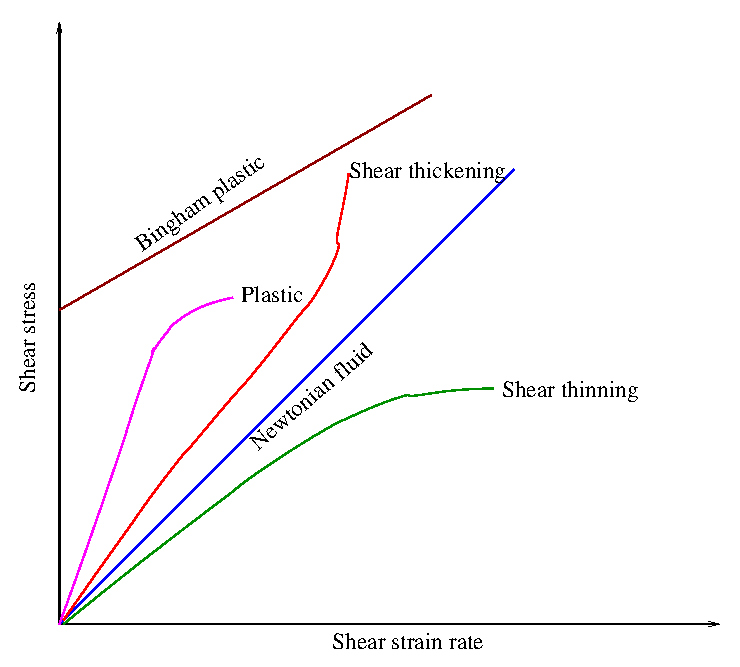
\includegraphics[width=5 in]{images/c10-fluidtypes.eps}
 % ctrans.eps: 46x0 pixel, 300dpi, 0.39x0.00 cm, bb=0 35 595 420
 \caption{Types of fluids}
 \label{fluidtypes}
\end{figure}

% learning objective
\begin{lo2}[Fluid Flow]
  List different types of fluids in contrast with Newtonian fluid
\end{lo2}

\begin{description}

\item[Newtonian fluid]: Strain rate or velocity gradient is linearly dependent on the shear stress as $\sigma_{12}=\mu u_{1,2}$. Eg: air and most of the gases, water, oils of low molecular weight and liquid metals. Often $\sigma_{12}$ is referred to as $\tau_{xy}$.

\item[Bingham Plastic]: Flow starts above a critical shear stress which is then linear with the strain rate. $\sigma_{12}= \sigma_{0} + \mu u_{1,2}$. Eg: drilling muds, peat slurries, margarine, chocolate mixtures, greases, soap, grain-water suspensions, toothpaste, paper pulp, and sewage sludge.

\item[Pseudoplastic]: Shear thinning material - viscosity decreases at higher strain rate. 

\item[Dilatant]: Shear thickening material - viscosity increases at higher strain rate.

\item[Thixotropic]: Viscosity decrease with time.

\item[Rheopectic]: Viscosity increases with time.

\item[Viscoelastic]: The material returns back to its original shape after the stress is removed.

\end{description}


\index{Viscosity}
Viscosity is a strong function of temperature. In liquid metals viscosity follows an {\em Arrhenius} relation. 
In situations where the temperature is roughly constant through out the flow, viscosity can be taken as constant. 
For fluids such as air and water, viscosity is negligible for most of the situations. Such fluids are called {\em inviscid}.  \index{Inviscid fluid}


\section{Reynold's number}

Consider the characteristic length scale of a domain to be $L$. This could be the diameter of a tube through which the fluid flows, the length along a plate over which the fluid flows, the separation between two walls between which the fluid flows and so on. Let $U_0$ be the characteristic velocity. This could be the maximum or average or externally imposed velocity. The characteristic time scale would then be $L/U_0$. Using these, the Navier-Stokes equation can be non-dimensionalized as follows. We take $x_1^* = {x_1 / L}$ as non-dimensionalized distance, $t^* = {t U_0 / L}$ as non-dimensionalized time etc. The non-dimensional velocities are $u_1^* = {u_1/U_0}$ etc.

$$ {\partial \over \partial x_1} = {\partial \over \partial x_1^*} {1 \over L}$$ 
$$ {\partial \over \partial t} = {\partial \over \partial t^*} {U_0 \over L}$$ 

Substitute these into the equation~\ref{nsa1} to obtain:

\begin{equation}
{U_0^2 \over L} \left[  \frac{\partial u_1^*}{\partial t^*} + u_1^* \frac{\partial u_1^*}{\partial x_1^*} + u_2^* \frac{\partial u_1^*}{\partial x_2^*} + u_3^* \frac{\partial u_1^*}{\partial x_3^*} \right] = F_1 -  \frac{1}{\rho L} \frac{\partial p}{\partial x_1^*} + \frac{\nu U_0}{L^2} \left( \frac{\partial^2 u_1^*}{\partial {x_1^*}^2} + \frac{\partial^2 u_1^*}{\partial {x_2^*}^2} + \frac{\partial^2 u_1^*}{\partial {x_3^*}^2} \right)
\end{equation} 

Gather the terms to obtain:

\begin{equation}
\frac{\partial u_1^*}{\partial t^*} + u_1^* \frac{\partial u_1^*}{\partial x_1^*} + u_2^* \frac{\partial u_1^*}{\partial x_2^*} + u_3^* \frac{\partial u_1^*}{\partial x_3^*} = \frac{L}{U_0^2} F_1 -  \frac{1}{\rho U_0^2} \frac{\partial p}{\partial x_1^*} + \frac{\nu}{L U_0} \left( \frac{\partial^2 u_1^*}{\partial {x_1^*}^2} + \frac{\partial^2 u_1^*}{\partial {x_2^*}^2} + \frac{\partial^2 u_1^*}{\partial {x_3^*}^2} \right)
\end{equation} 

Now we can consider that $U_0^2 / L$ as the scaling factor for $F_1$ so that non-dimensional force $F_1^* = {F_1 L / U_0^2}$. Similarly, the scaling factor for pressure can be taken as $\rho U_0^2$ so that non-dimensional pressure $p^* = {p / {\rho U_0^2}}$.


\begin{equation}
\frac{\partial u_1^*}{\partial t^*} + u_1^* \frac{\partial u_1^*}{\partial x_1^*} + u_2^* \frac{\partial u_1^*}{\partial x_2^*} + u_3^* \frac{\partial u_1^*}{\partial x_3^*} = F_1^* -  \frac{\partial p^*}{\partial x_1^*} + \frac{\nu}{L U_0} \left( \frac{\partial^2 u_1^*}{\partial {x_1^*}^2} + \frac{\partial^2 u_1^*}{\partial {x_2^*}^2} + \frac{\partial^2 u_1^*}{\partial {x_3^*}^2} \right)
\end{equation} 

The scaling factor for the diffusive term in the above equation can be taken as follows:

\begin{equation}
\boxed{ 
Re_L \equiv {L U_0 \over \nu} \equiv {L U_0 \rho \over \mu}
}
\end{equation}

Thus the non-dimensionalised Navier-Stokes equation for incompressible Newtonian fluid comes to be:

\begin{equation}
\frac{\partial u_1^*}{\partial t^*} + u_1^* \frac{\partial u_1^*}{\partial x_1^*} + u_2^* \frac{\partial u_1^*}{\partial x_2^*} + u_3^* \frac{\partial u_1^*}{\partial x_3^*} = F_1^* -  \frac{\partial p^*}{\partial x_1^*} + \frac{1}{Re_L} \left( \frac{\partial^2 u_1^*}{\partial {x_1^*}^2} + \frac{\partial^2 u_1^*}{\partial {x_2^*}^2} + \frac{\partial^2 u_1^*}{\partial {x_3^*}^2} \right)
\end{equation} 

The Reynold's number \index{Reynolds number} $Re_L$ is now a measure of the importance of the diffusive term in the Navier-Stokes equation while determining the fluid flow evolution. In the limit of $Re_L \to 0$ the flow field is expected to be governed mainly by the diffusive term. 


The subscript used with Reynold's number will be indicative of the characteristic length scale. A bar on the top, like $\bar{Re}$ indicates the use of average velocity for non-dimensionalization. 

% --------- end of nsderive2.tex ---------------------------------

%------ NSCylindrical.tex start -----------------
\section{Equations in cylindrical co-ordinate system}

We should choose a co-ordinate system with an orientation that best captures the symmetry of the problem and simplifies the final form of the solution.

Equations \ref{nsan} are written for constant properties ($\rho$ and $\mu$) and using the operators $\vnabla$ and $\nabla^2$. These operators convey a meaning independent of co-ordinate system and enable us to assign a meaning to each term in the equation. 

One can (with some endurance) derive the equations by expressing $x_1, x_2, x_3$ in terms of $r, \theta, z$ for cylindrical co-ordinate system or $r, \theta, \phi$ for spherical co-ordinate system and derive the necessary relations. The expansion of these operators and the N-S equations for cylindrical co-ordinate system can be borrowed from Appendix A of \cite{bls}. Following are the expressions that will be of use to us later. 

The velocity vector has the components as follows:

\begin{equation}
\vec{u} = u_r \hat{e}_r + u_\theta \hat{e}_\theta + u_z \hat{e}_z
\end{equation}

The operator $\vnabla$ is defined as:

\begin{equation}
\vnabla = \frac{\partial}{\partial r} \hat{e}_r + \frac{1}{r} \frac{\partial}{\partial \theta} \hat{e}_\theta + \frac{\partial}{\partial z} \hat{e}_z
\end{equation}

Remember the following relations before applying the operator directly:

\begin{equation}
{\partial \hat{e}_r \over \partial \theta} = \hat{e}_\theta
\end{equation}

\begin{equation}
{\partial \hat{e}_\theta \over \partial \theta} = -\hat{e}_r
\end{equation}

\subsection{Continuity equation}

Divergence of the velocity vector or continuity equation for an incompressible fluid is written as:

\begin{equation}
{1 \over r}{\partial \left( r u_r\right) \over \partial r} + {1 \over r}{\partial u_\theta \over \partial \theta} + {\partial u_z \over \partial z} = 0
\end{equation}

\subsection{Other operators}

The curl of velocity vector is given by the following:

\begin{equation}
\vnabla \times \vec{u} = \left[ {1 \over r}{\partial u_z \over \partial \theta} - {\partial u_\theta \over \partial z} \right] \hat{e}_r + \left[ {\partial u_r \over \partial z} - {\partial u_z \over \partial r} \right] \hat{e}_\theta + {1 \over r} \left[ {\partial \left( r u_\theta\right) \over \partial r} - {\partial u_r \over \partial \theta} \right] \hat{e}_z
\end{equation}

Laplacian operator for a scalar function can be given as:

\begin{equation}
\nabla^2 = {1 \over r} {\partial \over \partial r} \left( r {\partial \over \partial r} \right) + {1 \over r^2} {\partial^2 \over \partial \theta^2} + {\partial^2 \over \partial z^2}
\end{equation}

\begin{equation}
\vec{u} \cdot \vnabla = u_r \frac{\partial}{\partial r} + \frac{u_\theta}{r} \frac{\partial}{\partial \theta} + u_z \frac{\partial}{\partial z}
\end{equation}


\subsection{Stress components}

Normal and shear stresses for constant density and viscosity are given as follows:

\begin{equation}
\sigma_{rr} = -p + 2 \mu {\partial u_r \over \partial r}
\end{equation}

\begin{equation}
\sigma_{\theta \theta} = -p + 2 \mu \left[ {1 \over r} {\partial u_\theta \over \partial \theta} + {u_r \over r} \right]
\end{equation}

\begin{equation}
\sigma_{zz} = -p + 2 \mu {\partial u_z \over \partial z}
\end{equation}

\begin{equation}
\tau_{r\theta} = \mu \left[ r {\partial \over \partial r} \left( {u_\theta \over r} \right) + {1 \over r} {\partial u_r \over \partial \theta} \right]
\end{equation}

\begin{equation}
\tau_{\theta z} = \mu \left[ {\partial u_\theta \over \partial z} + {1 \over r} {\partial u_z \over \partial \theta} \right]
\end{equation}

\begin{equation}
\tau_{rz} = \mu \left[ {\partial u_r \over \partial z} + {\partial u_z \over \partial r} \right]
\end{equation}


\subsection{Navier-Stokes equations in cylindrical co-ordinate system}

Most of the time we are concerned about incompressible fluids of approximately constant properties. Hence we can borrow the N-S equations in cylindrical co-ordinate system for momentum transfer with these assumptions as reproduced below:

In these equations, kinematic viscosity $\nu \equiv { \mu / \rho}$ is used to simplify expressions.

\begin{align}
\frac{\partial u_r}{\partial t} + u_r \frac{\partial u_r}{\partial r} + \frac{u_\theta}{r} \frac{\partial u_r}{\partial \theta} + u_z \frac{\partial u_r}{\partial z} - \frac{u_\theta^2}{r} = F_r -\frac{1}{\rho}\frac{\partial p}{\partial r} \nonumber \\
+ \nu \left[ \frac{\partial}{\partial r}\left(\frac{1}{r} \frac{\partial \left\{r u_r\right\}}{\partial r} \right) + \frac{1}{r^2}\frac{\partial^2 u_r}{\partial \theta^2} - \frac{2}{r^2}\frac{\partial u_\theta}{\partial \theta} + \frac{\partial^2 u_r}{\partial z^2} \right] 
\end{align}

\begin{align}
\frac{\partial u_\theta}{\partial t} + u_r \frac{\partial u_\theta}{\partial r} + \frac{u_\theta}{r} \frac{\partial u_\theta}{\partial \theta} + \frac{u_r u_\theta}{r} + u_z \frac{\partial u_\theta}{\partial z} = F_\theta -\frac{1}{\rho r}\frac{\partial p}{\partial \theta} \nonumber \\
+ \nu \left[ \frac{\partial}{\partial r}\left(\frac{1}{r} \frac{\partial \left\{r u_\theta\right\}}{\partial r} \right) + \frac{1}{r^2}\frac{\partial^2 u_\theta}{\partial \theta^2} + \frac{2}{r^2}\frac{\partial u_r}{\partial \theta} + \frac{\partial^2 u_\theta}{\partial z^2} \right] 
\end{align}

\begin{align}
\frac{\partial u_z}{\partial t} + u_r \frac{\partial u_z}{\partial r} + \frac{u_\theta}{r} \frac{\partial u_z}{\partial \theta} + u_z \frac{\partial u_z}{\partial z} = F_z-\frac{1}{\rho}\frac{\partial p}{\partial z} \nonumber \\
+ \nu \left[ \frac{1}{r} \frac{\partial}{\partial r}\left( r \frac{\partial u_z}{\partial r} \right) + \frac{1}{r^2}\frac{\partial^2 u_z}{\partial \theta^2} + \frac{\partial^2 u_z}{\partial z^2} \right] 
\end{align}


%------ end of NSCylindrical.tex -----------------

\chapter{Specific cases of fluid flow - Planar}
\label{ch:flowprob}

\section{Learning objectives}

At the end of this lesson, a student should be able to

\begin{enumerate}
\item identify the domain, write down boundary conditions and list the allowed assumptions given a flow problem description
\item identify and justify terms of Navier-Stokes equation that can be dropped in a given problem
\item integrate simple partial differential equations across the domain of a flow problem
\item apply boundary conditions to determine integration constants of a flow field solution
\item plot velocity and stress profile across the domain for a flow problem
\end{enumerate}

\section{Boundary Conditions and Problem Definitions}

{\bf Fluid-Solid}: Due to van der Waals attractions, wetting and any other atomistic phenomena, liquid tends to stick to solid and a relative motion is not possible\footnote{except under situations where surface tension plays a major role}. In most of the situation this phenomena of a solid preventing a liquid in contact with it from having a motion relative to it is called \textit{no slip condition}. Often the solid wall is stationary making the velocity of liquid at the wall zero.
$$\left. u \right|_{\text{liquid, interface}} = \left. u \right|_{\text{solid}}$$

{\bf Fluid-Liquid}: Using the arguments similar to above, there is no relative motion between two layers of liquids in contact with each other\footnote{except in situations where the two liquids in contact with each other are immiscible and interfacial tension plays a major role}. Additionally, since most liquids wet each other, the shear stress at the interface of two liquids has a unique value. 
$$\left. \tau\right|_{\text{liquid1, interface}} = \left. \tau\right|_{\text{liquid2, interface}}$$
For Newtonian fluids, if we take the interface to be at zero,
$$\left. \mu_1 \frac{\partial u_i}{\partial x_j}\right|_{x_j \rightarrow -0} = \left.\mu_2 \frac{\partial u_i}{\partial x_j}\right|_{x_j \rightarrow +0} $$


{\bf Fluid-Gas}: Because the density of gas is usually much smaller than that of liquid, it cannot sustain any shear stress at the top of the liquid layer and will lead to surface deformation. Thus, the shear stress at a \textit{free surface} is zero.
$$\tau|_{\text{liquid, free surface}} = 0$$
For Newtonian fluids, if we take the interface to be at zero,
$$\left.\frac{\partial u_i}{\partial x_j}\right|_{x_j \rightarrow 0} = 0$$

Steady state: Time derivative of the velocity is to be taken zero.
$$\frac{\partial u_i}{\partial t} = 0$$

Unidirectional flow: Velocity has only one component and the other components are to be taken zero.
$$u_2 = u_3 = 0 \ne u_1$$

Fully developed flow: The velocity has no variation along the direction of the flow.
$$\frac{\partial u_i}{\partial x_i} = 0$$

Validity of solution: The analytical solutions given in this chapter are applicable for \textit{laminar regime} of fluid flow where the flow can be visualised as layers of liquid moving with respect to each other and the effects of wall penetrate far into the liquid. When the intertial forces acting on the fluid are far greater than the viscous forces, such an assumption is not valid and the flow is said to be \textit{turbulent}. A transition from \textit{laminar} to \textit{turbulent} regimes is governed by the non-dimensional number indicating the ratio of intertial to viscous forces and is named after \textbf{Reynolds}.
$$Re = \frac{\rho D u_0}{\mu} = \frac{D u_0}{\nu}$$

$D$ is the characteristic length scale (diameter for a tube flow, width of channel for flow between two parallel plates etc.,), $u_0$ is the characteristic velocity (typically the average velocity or far field velocity) and $\nu$ is the kinematic viscosity.

Range of $Re$ for validity of a laminar solution for a problem of certain geometry is obtained from careful experiments.


Equivalent diameter: For tubes of non-circular cross sections or for other geometries, the equivalent diameter can be defined as 
$$ D_e = \frac{4 \times \text{cross sectional area}}{\text{wetted perimeter}}$$

Thus, for the case of flow between two parallel plates separated by a distance of $2\delta$ that is much smaller than the width of the plates $W$, $D_e = 4\delta$.

\section{Trivial case reproducing Newton's Law}

\begin{figure}[h]
\begin{center}
\framebox{ 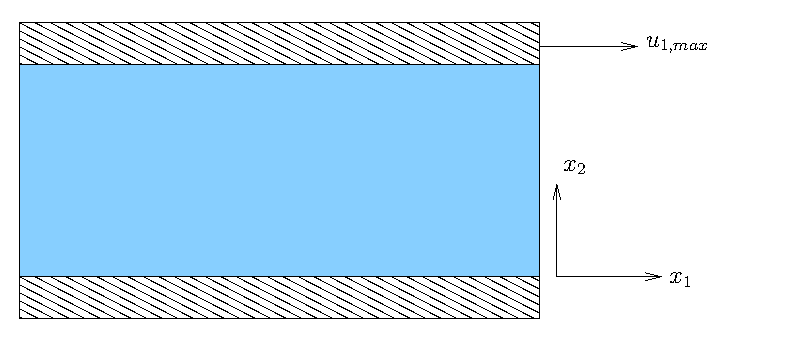
\includegraphics[scale=1]{images/c11-nlawfig.ps}}
\end{center}
\caption{Problem domain to recover Newton's Law}
\label{nlawfig}
\end{figure}

Figure \ref{nlawfig} shows the problem definition.


Assumptions:
\begin{itemize}
\item Flow is unidirectional. Only $u_1$ is to be known, $u_2$ and $u_3$ are zero.
\item Flow is steady state. $\frac{\partial u_1}{\partial t} = 0$.
\item Flow is fully developed. $\frac{\partial u_1}{\partial x_1} = 0$.
\item Flow is entirely due to the top surface being moved at $u_{1,max}$ and no body force or pressure gradients exist.
\end{itemize}


Boundary Conditions:
\begin{itemize}
\item No slip condition at bottom layer: at $y=0$, $u_1=0$.
\item No slip condition at top layer: at $y=\delta$, $u_1=u_{1,max}$.
\end{itemize}


Solution:
Use N-S equation for $u_1$ and eliminate terms as per the assumptions above.

\begin{equation}
\frac{\partial u_1}{\partial t} + u_1\frac{\partial u_1}{\partial x_1} + u_2\frac{\partial u_1}{\partial x_2} + u_3\frac{\partial u_1}{\partial x_3} = F_1 -  \frac{1}{\rho}\frac{\partial p}{\partial x_1} + \nu \left( \frac{\partial^2 u_1}{\partial x_1^2} + \frac{\partial^2 u_1}{\partial x_2^2} + \frac{\partial^2 u_1}{\partial x_3^2} \right)
\end{equation} 

\begin{equation}
\nu \frac{\partial^2 u_1}{\partial x_2^2} = 0 
\end{equation} 
or
\begin{equation}
u_1 = A x_2 + B 
\end{equation} 

Using the boundary conditions,

$$A = \frac{u_{1,max}}{\delta}$$
$$B = 0$$
or
$$u_1 = u_{1,max} \frac{y}{\delta}$$

Using Newton's law $$\sigma_{21} = \tau_{yx} = \mu \frac{\partial u_1}{\partial x_2}$$

$$\tau_{yx} = \mu \frac{u_{1,max}}{\delta}$$

The solution is plotted schematically in figure \ref{nlawsolfig}.

\begin{figure}[h]
\begin{center}
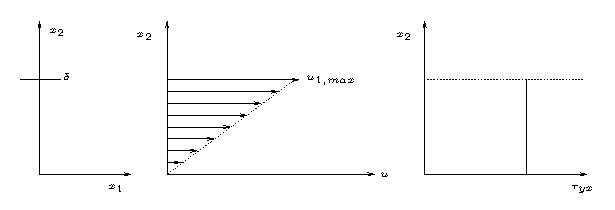
\includegraphics[scale=1.0]{images/c11-nlawsolfig.ps}
\end{center}
\caption{Velocity and Stress distribution in the Newton's Law problem}
\label{nlawsolfig}
\end{figure}

Convention: $\sigma_{12}$ or $\tau_{12}$ is on plane $1$ and in the direction $2$. As for the sign, there are two different convections adapted in the literature. 


{\bf Convention +}: 

In the above case, we have used the convention that the shear stress is positive and it is exerted by the top layer on the fluid beneath it so that Newton's law is written as $\tau_{21} = \mu \frac{\partial u_1}{\partial x_2}$.  

Shear stress $\tau_{yx}$ is stress exerted on plane $y$ in the positive direction $x$ by the layer at {\em greater} $y$ on the layer at {\em lesser} $y$.

This is the convention adapted in this handout.

{\bf Convention -}: 

This is favoured by \cite{bls} for the reasons quoted below. 

Shear stress $\tau_{xy}$ is stress exerted on plane $x$ in direction $y$ by the layer at {\em lesser} $y$ on the layer at {\em greater} $y$.

Quoting from \cite{bls} section 1.2, page 19:

\hspace{0.1\linewidth}\begin{minipage}[t]{0.8\linewidth}
{\em Note on the Sign Convention for the Stress Tensor} We have emphasised in connection with Eq. 1.1-2 (and in the generalization in this section) that $\tau_{yx}$ is the force in the positive $x$ direction on a unit area perpendicular to the $y$ direction, this being the force per unit area exerted by the fluid in the region of the {\it lesser} $y$ on the fluid of {\it greater} $y$. In most fluid dynamics and elasticity books, the words "lesser" and "greater" are interchanged and Eq 1.1-2 is written as $\tau_{yx} = +\mu(dv_x/dy)$. The advantages of the sign convention used in this book are: (a) the sign convention used in Newton's law of viscosity is consistent with that used in Fourier's law of heat conduction and Fick's law of diffusion; (b) the  sign convention used for $\tau_{ij}$ is the same as that for convective momentum flux $\rho \mathbf{v} \mathbf{v}$ (see section 1.7 and Table 19.2-2); (c) in Eq 1.2-2, the terms $p\delta_{ij}$ and $\tau_{ij}$ have the same sign affixed, and the terms $p$ and $\tau_{ii}$ are both positive in compression (in accordance with common usage in thermodynamics); (d) all terms in the entropy production in Eq. 24.1-5 have the same sign. Clearly the sign convention in Eqs. 1.1-2 and 1.2-6 is arbitrary, and either sign convention can be used, provided the physical meaning of the sign convention is clearly understood.
\end{minipage}

{\bf Note}: Figure 2.8 of~\cite{gaskell} shows a symmetric plot of velocity profile as well as shear stress profile for a channel flow. There is an error in the shear stress profile. Watch out!

%%%%%%%%%%%%%%%%%%%%%%%%%%%%%%%%%%%%%%%%%%%%%%%%%%%%%%%%%%%%%%%%%%%%%%%%%%

\section{Film flow}

Consider the case of a film of liquid falling on an inclined plane as shown in figure \ref{fallfilm}.

\begin{figure}[h]
\begin{center}
\framebox{\resizebox{4in}{!}{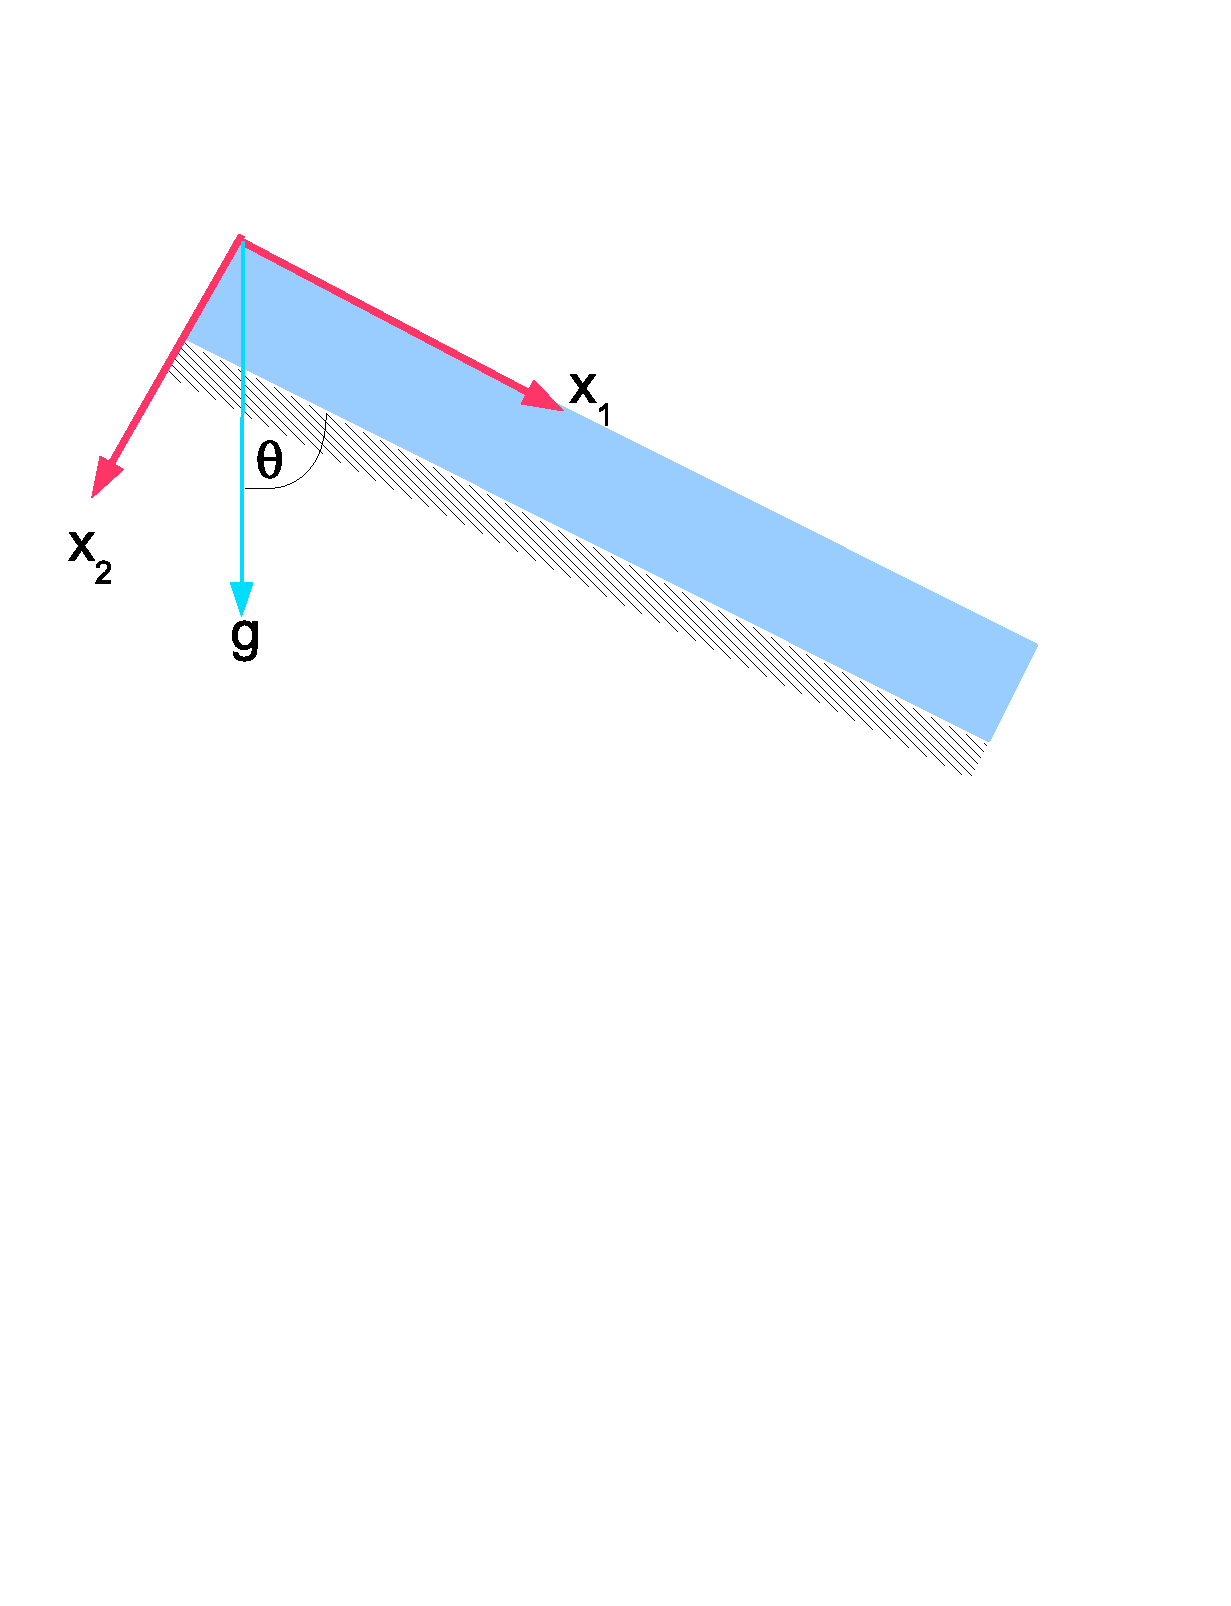
\includegraphics[bb=20 383 545 675, clip]{images/c11-FallingFilm.eps}}}
\end{center}
\caption{Schematic of a film flow problem}
\label{fallfilm}
\end{figure}


Assumptions:
\begin{itemize}
\item Flow is unidirectional. Only $u_1$ needs to be known, $u_2=u_3=0$.
\item Flow is steady state: $\frac{\partial u_1}{\partial t}=0$.
\item Flow is fully developed i.e., it varies only along $x_2$ but not along $x_1$ or $x_3$. $\frac{\partial u_1}{\partial x_1} = 0$ for all $x_1$. 
\item The only driving force for the film to fall is gravity: $\vec{F} = g\cos\theta \hat{x_1} + g\sin\theta \hat{x_2}$.
\end{itemize}


Boundary conditions:
\begin{itemize}
\item Thickness of the film is $\delta$.
\item No slip condition at the bottom of the plane: at $x_2= \delta$, $u_1=0$.
\item At $x_2 = 0$, there is a free surface on which the shear stresses are zero. $\mu \frac{\partial u_1}{\partial x_2}=0$ at $x_2 = 0$.
\end{itemize}


Solution:
Use N-S equation for $u$ and eliminate terms as per the assumptions above.

\begin{equation}
\frac{\partial u_1}{\partial t} + u_1\frac{\partial u_1}{\partial x_1} + u_2\frac{\partial u_1}{\partial x_2} + u_3\frac{\partial u_1}{\partial x_3} = F_1 -  \frac{1}{\rho}\frac{\partial p}{\partial x_1} + \nu \left( \frac{\partial^2 u_1}{\partial x_1^2} + \frac{\partial^2 u_1}{\partial x_2^2} + \frac{\partial^2 u_1}{\partial x_3^2} \right)
\end{equation} 

\begin{equation}
0 =  g \cos\theta + \nu \frac{\partial^2 u_1}{\partial x_2^2} 
\end{equation} 


$$ \frac{\partial^2 u_1}{\partial x_2^2} = -\frac{\rho g \cos\theta}{\mu} $$

$$ u_1 = -\frac{\rho g \cos\theta x^2_2}{2\mu} + C_1 x_2 + C_2 $$

Using the boundary conditions, $C_1 = 0$.

$$ C_2 = \frac{\rho g \cos\theta \delta^2}{2\mu} $$ 
Hence,
$$ u_1 = \frac{\rho \delta^2 g\cos\theta }{2 \mu}\left[1-\left(\frac{x_2}{\delta}\right)^2\right]$$

$$u_1|_{max} = \frac{\rho \delta^2 g\cos\theta}{2 \mu}$$

Using Newton's law $$\sigma_{21} = \tau_{yx} = \mu \frac{\partial u_1}{\partial x_2}$$

$$\tau_{yx} = -\rho g \cos\theta x_2$$


$$\bar{u}_1 = \frac{\int_0^\delta{u_1}dx_2}{\delta} = \frac{\rho \delta^2 g\cos\theta}{3 \mu} = \frac{2}{3} u_1|_{max}$$

If $W$ is the width of the plane, mass flow rate $\dot{M}$ is:

$$ \dot{M} = \rho W \delta \bar{u}_1 = \frac{\rho^2 \delta^3 W g \cos\theta}{3 \mu}$$

The solutions are plotted schematically in figure \ref{fallfilmsol}.

\begin{figure}[h]
\begin{center}
\framebox{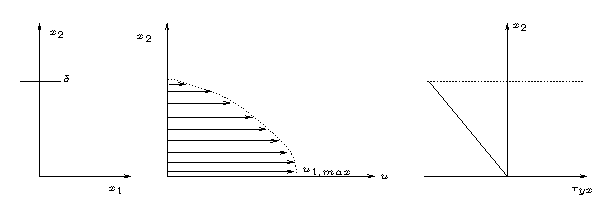
\includegraphics[scale=1.0]{images/c11-fallfilmsolfig.ps}}
\end{center}
\caption{Velocity and Stress distribution in a film flow problem}
\label{fallfilmsol}
\end{figure}


Validity:
$$Re = \frac{4\delta \rho \bar{u}_1  }{\mu} \le 25$$ 

%%%%%%%%%%%%%%%%%%%%%%%%%%%%%%%%%%%%%%%%%%%%%%%%%%%%%%%%%%%%%%%%%%%%%%%%%%

\section{Flow between two plates}

\begin{figure}[h]
\begin{center}
\framebox{
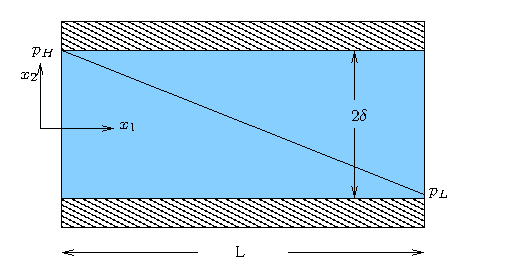
\includegraphics[scale=1.0]{images/c11-pchannelfig.ps}
}
\end{center}
\caption{Flow in a channel}
\label{pchannel}
\end{figure}

Figure \ref{pchannel} shows the problem definition. We choose the axes to make the maximum out of the symmetry of the problem.

Assumptions:
\begin{itemize}
\item Flow is unidirectional. Only $u_1$ is to be known, $u_2$ and $u_3$ are zero.
\item Flow is steady state. $\frac{\partial u_1}{\partial t} = 0$.
\item Flow is fully developed. $\frac{\partial u_1}{\partial x_1} = 0$.
\item Pressure gradient is constant $-\frac{\partial p}{\partial x_1} = \frac{p_H - p_L}{L}$
\end{itemize}

Boundary Conditions:
\begin{itemize}
\item No slip condition at bottom layer: at $y=-\delta$, $u_1=0$.
\item No slip condition at top layer: at $y=\delta$, $u_1=0$.
\end{itemize}

Use N-S equation for $u_1$ and eliminate terms as per the assumptions above.

\begin{equation}
\frac{\partial u_1}{\partial t} + u_1\frac{\partial u_1}{\partial x_1} + u_2\frac{\partial u_1}{\partial x_2} + u_3\frac{\partial u_1}{\partial x_3} = F_1 -  \frac{1}{\rho}\frac{\partial p}{\partial x_1} + \nu \left( \frac{\partial^2 u_1}{\partial x_1^2} + \frac{\partial^2 u_1}{\partial x_2^2} + \frac{\partial^2 u_1}{\partial x_3^2} \right)
\end{equation} 

\begin{equation}
\nu \frac{\partial^2 u_1}{\partial x_2^2} = \frac{1}{\rho}\frac{\partial p}{\partial x_1} = \frac{p_L-p_H}{\rho L} 
\end{equation} 
or
\begin{equation}
\frac{\partial^2 u_1}{\partial x_2^2} = -2A 
\end{equation} 

$$A = \frac{p_H-p_L}{2L \mu}$$

$$u_1 = -A x_1^2 + B x_1 + C$$

Using the boundary conditions,

$$\boxed{u_1 = \frac{p_H - p_L}{L} \frac{\delta^2 -x_2^2}{2\mu} }$$

Using Newton's law $$\sigma_{21} = \tau_{21} = \mu \frac{\partial u_1}{\partial x_2}$$

$$\tau_{21} = \frac{p_H - p_L}{2 L} \left( -2x_2 \right)$$

Maximum velocity:
$$\boxed{u_1|_{max} = \frac{p_H - p_L}{L} \frac{\delta^2}{2 \mu}} $$

Average velocity:
$$\boxed{ \bar{u}_1 = \frac{2}{3} u_1|_{max}  = \frac{p_H - p_L}{L} \frac{\delta^2}{3 \mu} }$$


The solutions are plotted schematically in figure \ref{chansol}.

\begin{figure}[h]
\begin{center}
\framebox{
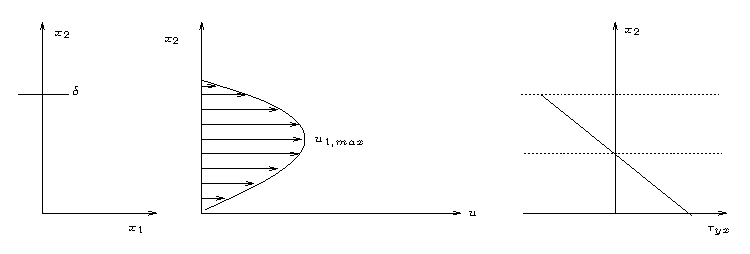
\includegraphics[scale=1.0]{images/c11-chansolfig.ps}
}
\end{center}
\caption{Flow in a channel}
\label{chansol}
\end{figure}

Interpretation of $\tau_{21}$. At $x_2=0$, $\tau_{21} = + A \mu \delta$. Recollecting {\bf convention +} we are using for Newton's law, the shear stress is exerted by the layer at {\em greater} $x_2$ on the layer at {\em lesser} $x_2$ ie., by the liquid on the wall.
At $x_2=\delta$, $\tau_{21} = - A \mu \delta$. The shear stress is exerted by the layer at {\em greater} $x_2$ on the layer at {\em lesser} $x_2$ ie., by the wall on the liquid (thus the negative sign). 

%%%%%%%%%%%%%%%%%%%%%%%%%%%%%%%%%%%%%%%%%%%%%%%%%%%%%%%%%%%%%%%%%%%%%%%%%%

% ------------------------------------------------------------------------------
\begin{figure}[h]
\begin{center}
\frame{
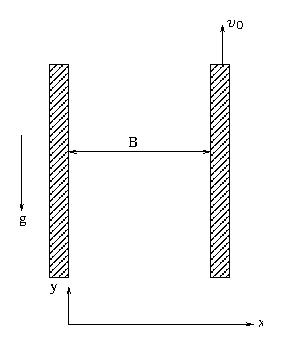
\includegraphics[scale=1.0]{images/c11-mixingfilmfig.ps}
}
\end{center}
\caption{Schematic of a film mixing problem}
\label{MixingFilm}
\end{figure}

\begin{question} 
\item Mixing film: Problem 2B.3 and 2B.4 of~\cite{bls}. An incompressible Newtonian fluid is contained between two long plates of width $W$ = \SI{1}{\metre} (along $z$) and  a distance $B$ = \SI{1}{\mm} apart as shown in figure~\ref{MixingFilm} below. The plate on the right is moved upwards at a velocity $v_0$. Gravity $g$ = \SI{9.81}{\mpss} acts along $y$ axis downwards, density of fluid $\rho$ = \SI{1000}{\kgpmc} and viscosity of fluid \SI{0.01}{\pas}. Assume  the flow is uniaxial, steady state and fully developed. (a) Calculate $v_0$ such that the net volume flow rate across a $y$ plane is zero. (b) What is the ratio of the width of the fluid layer that flows downwards to the width of the fluid layer that flows upwards. (c) Sketch a schematic of the flow field.
\end{question}
\begin{solution}[print]
\end{solution}

% ------------------------------------------------------------------------------

\begin{question} 
Slag film: Problem 2.5 of~\cite{gaskell}. A layer of molten slag of density \SI{2700}{\kgpmc} and viscosity \SI{0.3}{\pascal\second} is being transferred from one reverberatory furnace to another by flow down a plane between the two furnaces inclined at $10^o$ to the horizontal. The plane is \SI{5}{\metre} in width and \SI{5}{\metre} in length and the mass flow rate of the slag is \SI{7.5}{\kilo\gram\per\second}. Neglecting the end effects, calculate (a) thickness of the slag layer (b) average linear flow velocity of the slag and (c) mean residence time of slag on the plane. (d) Fraction of slag that remains on the plane for times equal to or greater than the mean residence time.
\end{question}
\begin{solution}[print]
{\it Answer}: 
(a) \SI{4.77e-3}{\kilo\gram\per\metre\per\second}
(b) \SI{0.116}{\metre\per\second}
(c) \SI{43}{\second}
(d) \num{0.423}
\end{solution}

% ------------------------------------------------------------------------------

\begin{figure}[h]
\label{squeegee}
\begin{center}
\resizebox{!}{3in}{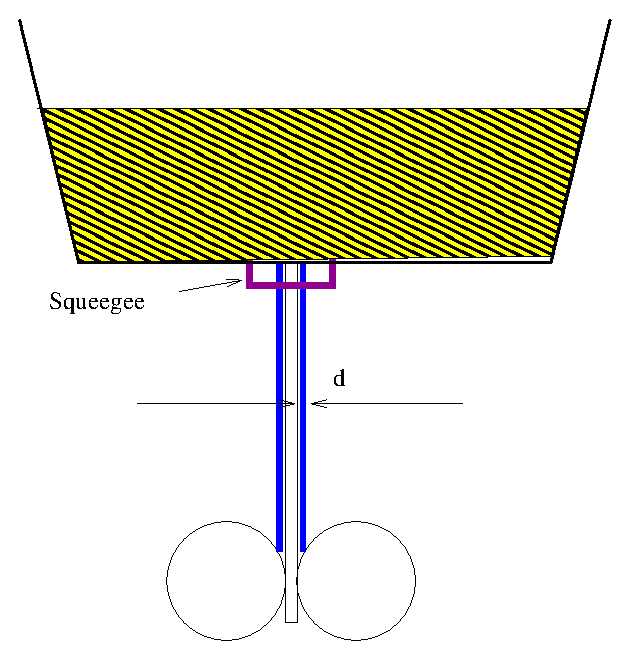
\includegraphics[bb=0 0 287 300, clip]{images/c11-squeegee.eps}}
\end{center}
\caption{Squeegee device}
\end{figure}

\begin{question} 
Squeegee device: A continuous sheet (\SI{1.5}{\metre} wide) of metal is cold-rolled by passing vertically between rolls at a constant speed of \SI{0.3}{\metre\per\second}. Before entering the rolls, the sheet passes through a tank of lubricating oil equipped with a squeegee device that coats both sides of the sheet uniformly as it exits. The amount of oil that is carried through can be controlled by the squeegee device. Determine the mass rate of oil as a function of thickness of oil film that usually range between \SI{0}{\milli\metre} and \SI{0.6}{\milli\metre}. Properties of the lubricating oil: $\rho$ = \SI{962}{\kilo\gram\per\metre\cubed}, $\mu$ = \SI{4.1e-3}{\pascal\second}.
\end{question}
\begin{solution}[print]
\end{solution}

% --------------- end of momcases-planar.tex --------------------------------------------


\chapter{Specific cases of fluid flow - Cylindrical}
\label{ch:momcasescyl}

\section{Flow through a pipe}

\begin{figure}[h]
\begin{center}
\framebox{
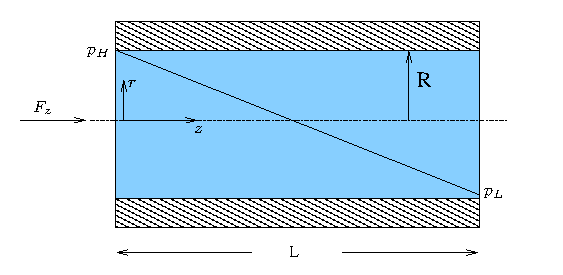
\includegraphics[scale=1.0]{images/c12-pipeflowfig.ps}
 }
\end{center}
\caption{Pipe Flow}
\label{pipeflow}
\end{figure}

Figure \ref{pipeflow} shows the problem definition.


Assumptions:
\begin{itemize}
\item Flow is unidirectional: Only $u_z$ is to be known, $u_r$ and $u_\theta$ are zero
\item Flow is steady state: $\frac{\partial u_z}{\partial t} = 0$
\item Flow is fully developed: $\frac{\partial u_z}{\partial z} = 0$
\item Pressure gradient is constant: $\frac{\partial p}{\partial z} = \frac{\Delta p}{L}$
\end{itemize}


Boundary Conditions:
\begin{itemize}
\item No slip condition at pipe wall: at $r=R$, $u_z=0$.
\item Finite velocity at center: at $r=0$, $u_z \ne \infty$.
\end{itemize}


Use N-S equation in cylindrical co-ordinate system for $u_z$ and eliminate terms as per the assumptions above.

\begin{align}
\frac{\partial u_z}{\partial t} + u_r \frac{\partial u_z}{\partial r} + \frac{u_\theta}{r} \frac{\partial u_z}{\partial \theta} + u_z \frac{\partial u_z}{\partial z} = F_z-\frac{1}{\rho}\frac{\partial p}{\partial z} \nonumber \\
+ \nu \left[ \frac{1}{r} \frac{\partial}{\partial r}\left( r \frac{\partial u_z}{\partial r} \right) + \frac{1}{r^2}\frac{\partial^2 u_z}{\partial \theta^2} + \frac{\partial^2 u_z}{\partial z^2} \right] 
\end{align}

\begin{equation*}
0 = F_z-\frac{1}{\rho}\frac{\Delta p}{L} + \frac{\mu}{\rho} \frac{1}{r} \frac{\partial}{\partial r}\left( r \frac{\partial u_z}{\partial r} \right)  
\end{equation*}

\begin{equation*}
u_z  = -\left[ \frac{\rho F_z}{4 \mu}-\frac{1}{4\mu}\frac{\Delta p}{L} \right] r^2 + C_1 \ln(r) + C_2
\end{equation*}

Using boundary conditions,
$$C_1 = 0$$
\begin{equation*}
C_2  = \left[ \frac{\rho F_z}{4 \mu}-\frac{1}{4\mu}\frac{\Delta p}{L} \right] R^2 
\end{equation*}

\begin{equation*}
u_z = \left[ \frac{\rho F_z}{4 \mu}-\frac{1}{4\mu}\frac{\Delta p}{L} \right] (R^2 - r^2)
\end{equation*}

Using Newton's law $$\sigma_{21} = \tau_{zr} = \mu \frac{\partial u_z}{\partial r}$$

$$\tau_{zr} = \left[ \frac{\rho F_z}{4 \mu}-\frac{1}{4\mu}\frac{\Delta p}{L} \right] (-2r) $$

The solution is plotted schematically in figure \ref{pfslfg}.

\begin{equation*}
u_z|_{max} = \left[ \frac{\rho F_z}{4 \mu}-\frac{1}{4\mu}\frac{\Delta p}{L} \right] R^2
\end{equation*}

Average flow velocity $\bar{u}_z$:
$$ \bar{u}_z = \frac{\int_0^R{u_z 2\pi r dr}}{\int_0^R{2\pi r dr}} = \frac{1}{2} u_z|_{max}$$
Volume flow rate $\dot{V}$:
$$ \dot{V} = \pi r^2 \bar{u}_z = \left[ \frac{\rho F_z}{8 \mu}-\frac{1}{8\mu}\frac{\Delta p}{L} \right] \pi R^4 $$

Mass flow rate $\dot{M}$ (Hagen-Poiseuille Equation):
$$ \boxed{\dot{M} = \rho \dot{V} = \left[ \frac{\rho^2 F_z}{8 \mu}-\frac{\rho}{8\mu}\frac{\Delta p}{L} \right] \pi R^4} $$

\begin{figure}[h]
\begin{center}
\framebox{
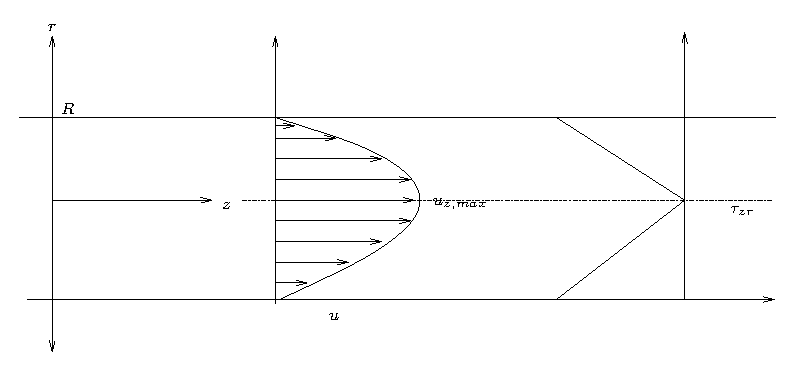
\includegraphics[scale=1.0]{images/c12-pipeflowsolfig.ps}
}
\end{center}
\caption{Solution to Pipe Flow}
\label{pfslfg}
\end{figure}

% --------------------------------------------------------------------
\begin{figure}[h]
\label{axialfilmflow}
\begin{center}
\frame{
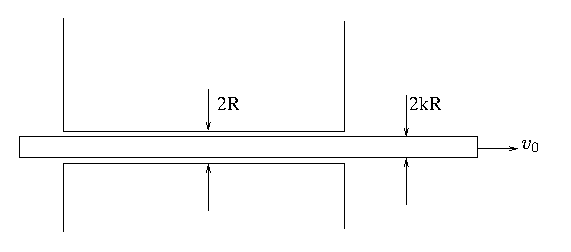
\includegraphics[scale=1.0]{images/c12-filmflowfig.ps}
}
\end{center}
\caption{Axial film flow}
\end{figure}

\begin{question}
Axial film flow: Problem 2B.7 of~\cite{bls}. A cylindrical rod of radius $kR$ moves axially with velocity $v=v_0$ along the axis of a cylindrical cavity of radius $R$ as shown in figure below. Assuming that the pressure at both ends of the cavity is same and fluid flows through the annular region only because of the rod motion. (a) Find the velocity distribution in the narrow annular region. (b) Find the mass flow rate through the annular region. (c) Obtain the viscous force acting on the rod over a length L.\\
\end{question}
\begin{solution}[print]
(a) $$ {u_z \over u_0} = { \ln \left( r / R \right) \over \ln k} $$
(b) $$ \dot{M} = {\pi R^2 u_0 \rho \over 2} \left( {1 - k^2 \over \ln \left(1 /k\right)} - 2 k^2 \right)$$
(c) $$ F_z = {2 \pi L \mu u_0 \over \ln \left( 1 / k \right)} $$
\end{solution}

% --------------------------------------------------------------------

\begin{figure}[h]
\begin{center}
\frame{
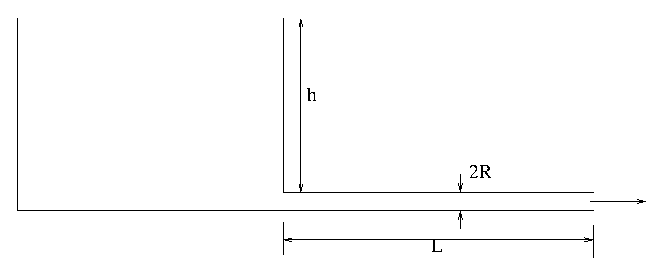
\includegraphics{images/c12-LeakingTank.eps}
}
\end{center}
\caption{Leaking Tank}
\label{LeakingTank}
\end{figure}

\begin{question}
Leaking tank: Water of viscosity $\mu$ = \SI{0.01}{\pascal\second} and density $\rho$ = \SI{1000}{\kilo\gram\per\metre\cubed} from a large tank is to be transported using a rigid smooth tube of \SI{1}{\centi\metre} dia connected at the bottom across a distance of $L$ = \SI{100}{\metre} as shown in figure~\ref{LeakingTank}. Assuming that at steady state the tank is large enough that the height of water in it ($h$) does not change much in time, what should be $h$ such that the flow rate in the tube is one litre per minute. 
\end{question}
\begin{solution}[print]
\end{solution}

% --------------------------------------------------------------------
\begin{figure}[h]
\begin{center}
\resizebox{5in}{!}{\includegraphics[bb=0 0 210 149, clip]{images/c12-CubicPipeNetwork2.eps}}
\end{center}
\caption{Cubic network of pipes}
\label{CubicPipeNetwork}
\end{figure}

\begin{question}
Cubic network of pipes: Problem 2B.12 of~\cite{bls}. A fluid is flowing in laminar flow from A to B through a network of tubes, as depicted in figure~\ref{CubicPipeNetwork}. Obtain an expression for the mass flow rate $w$ of the fluid entering at A (or leaving at B) as a function of the modified pressure drop $p_A - p_B$. Neglect the disturbances at the various tube junctions. Neglect any body forces that may act on some of the segments due to their orientation.\\
\end{question}
\begin{solution}[print]
Writing volume flow rate through each pipe at junctions as follows:

At junction 2:
$$ V_{A2} = V_{26} + V_{24}$$
	$${p_2 - p_A \over L} D^4 { \pi \over 8 \mu} = {p_6 - p_2 \over L} D^4 {\pi \over 8 \mu}  + {p_4 - p_2 \over L} D^4 {\pi \over 8 \mu} $$
$$ p_A = 3 p_2 -p_4 -p_6 $$

Skip the term $ {D^4 \pi \over L 8 \mu}$ for the remaining equations.

At junction 3:
$$ V_{A3} = V_{36} + V_{35}$$
$$ \left( p_3 - p_A \right) = \left( p_6 - p_3 \right) + \left( p_5 - p_3 \right) $$
$$ p_A = 3 p_3 -p_5 -p_6 $$

At junction 6:
$$ V_{36} + V_{26} = V_{6B}$$
$${p_6 - p_3 \over L} D^4 + {p_6 - p_2 \over L} D^4 = {p_B - p_6 \over L} D^4 $$
$$ p_B = 3 p_6 -p_2 -p_3 $$

Add the above three to obtain:

$$ 3p_B = 3 \left( p_4 + p_5 + p_6 \right) - 2 \left( p_1 + p_2 + p_3\right)$$

At junction 5:
$$ V_{35} + V_{15} = V_{5B}$$
$${p_5 - p_3 \over L} D^4 + {p_5 - p_1 \over L} D^4 = {p_B - p_5 \over L} D^4 $$
$$ p_B = 3 p_5 -p_3 -p_1 $$

At junction 1:
$$ V_{A1} = V_{15} + V_{14}$$
$${p_1 - p_A \over L} D^4 = {p_5 - p_1 \over L} D^4 + {p_4 - p_1 \over L} D^4 $$
$$ p_A = 3 p_1 -p_4 -p_5 $$


At junction 4:
$$ V_{14} + V_{24} = V_{4B}$$
$${p_4 - p_1 \over L} D^4 + {p_4 - p_2 \over L} D^4 = {p_B - p_4 \over L} D^4 $$
$$ p_B = 3 p_4 -p_1 -p_2 $$

Add the above three to obtain:

$$ 3p_A = 3 \left( p_1 + p_2 + p_3 \right) - 2 \left( p_4 + p_5 + p_6\right)$$

Write the flow rate at junction A:
$$ V_A = V_{A1} + V_{A2} + V_{A3}$$
$$ V_A = \left( p_1 - p_A + p_2 - p_A + p_3 - p_A \right) {D^4 \over L} { \pi \over 8 \mu} $$
$$ V_A = \left( p_1 + p_2 + p_3 - 3 p_A \right) {D^4 \over L} { \pi \over 8 \mu} $$

Multiply the equations with 2 and 3 to add to eliminate $ p_4 + p_5 + p_6$ term and give:

$$ 6 p_B + 9 p_A = 6 \left( p_4 + p_5 + p_6 \right) - 4 \left( p_1 + p_2 + p_3 \right) + 9 \left( p_1 + p_2 + p_3 \right) - 6 \left( p_4 + p_5 + p_6 \right)$$
$$ 6 p_B + 9 p_A = 5 \left( p_1 + p_2 + p_3 \right) $$

Now, using the equation for $V_A$, we can write:

$$ V_A = \left({ { 6p_B + 9 p_A} \over 5} - 3 p_A \right) {D^4 \over L} { \pi \over 8 \mu} $$
$$ V_A = {6 \pi \over 40 \mu} \left( p_B - p_A \right) {D^4 \over L} $$
$$ V_A = {3 \pi \over 20 \mu} \left( p_B - p_A \right) {D^4 \over L} $$

$$\dot{M} = {3 \pi \left( p_A - p_B \right) R^4 \rho \over 20 \mu L}$$
\end{solution}

% --------------------------------------------------------------------

\begin{question}
Blasius equation: Section 4.1 of~\cite{gaskell}. For steady viscous flow through a circular tube, the axial velocity profile is given approximately by the Blasius' equation below.
$$ u = u_0 \left( 1 - {r \over R} \right)^m$$
For turbulent flow, $m = {1 / 7}$. Assuming the density is constant, what is the average velocity? Is it closer to the maximum than in the case of Poiseuille flow? Comment.\\
\end{question}
\begin{solution}[print]
$0.817 u_0$
\end{solution}

% --------------------------------------------------------------------
\begin{figure}[h]
\begin{center}
\frame{
\includegraphics[scale=1.0]{images/c12-porouschannelfig.ps}
}
\end{center}
\caption{Channel flow between porous walls}
\label{PorousChannel}
\end{figure}

\begin{question}
Channel flow between porous walls: Problem 3B.16 of~\cite{bls}. Newtonian fluid flows through a rectangular channel with porous walls with a height $h$ and infinite extensions along $x_1$ and $x_3$ directions as shown in figure~\ref{PorousChannel}. The fluid leaks through the walls at a constant velocity of $v_w$. The plane flow is steady, density $\rho$ and viscosity $\mu$ are constant and there are no body forces. The flow takes place due to a constant pressure gradient $\Delta p \over L$. Velocity is fully developed along $x_1$. (a) Use the continuity equation to obtain $u_2(x_2)$. (b) Write the Navier-Stokes equation for $u_1$ after simplification. (c) Assuming no slip boundary conditions applicable for $u_1$, show that the velocity distribution can be given by the expression below.
 (d) Show that in the limit $v_w \rightarrow 0$, we retrieve the velocity profile of a plane channel flow. Note the location of axes different from the ones used in the class.
$$u_1(x_2) = {\Delta p \over L} {h \over \rho v_w} \left( {x_2 \over h} - {{1- e^{v_w x_2 \over \nu}} \over {1 - e^{v_w h \over \nu}}} \right)$$
\end{question}
\begin{solution}[print]
\end{solution}

% --------------------------------------------------------------------

\begin{question}
Euler equation: Euler equation governs the flow of inviscid fluids i.e., fluids with nearly zero viscosity. (a) Use the information given at the end of the question paper and write down Euler equation in one dimension case for flow in a vertical tube due to both gravity as well as pressure gradient. (b) Show that in steady state, it reduces to the following expression popularly known as Bernouli equation.
$$ \frac{p}{\rho} + gz + \frac{v_z^2}{2} = \text{constant}$$
\end{question}
\begin{solution}[print]
\end{solution}

% --------------------------------------------------------------------

\begin{question}
Couette flow: The Navier-Stokes equation for the $\theta$ component of velocity in cylindrical coordinate system is given to you. Annular region between two coaxial cylindrical surfaces of radii $r_i$ and $r_o$ (for inner and outer radii, respectively) is filled with a fluid. The outer cylinder is rotating with an angular velocity of $\Omega_o$ and the inner cylinder is rotating with an angular velocity of $\Omega_i$, both clockwise. Assume that the fluid flow is uniform, steady state and fully developed and is only due to the rotation of outer cylinder. (a) Determine the velocity distribution in the liquid in the annular region. (b) Show that the result will approximate to Newton's Law when the difference of radii is very small compared to either radii.
\end{question}
\begin{solution}[print]
\end{solution}

% --------------------------------------------------------------------

\begin{question}
Channel flow of two stratified immiscible fluids: Section 2.5 of~\cite{bls}. Two immiscible incompressible fluids of viscosities $\mu_1$ (bottom) and $\mu_2$ (top) are flowing between two stationary parallel plates under a pressure gradient $\Delta P \over L$. Assume $\mu_1 > \mu_2$. The thickness of the two layers $\delta$ is same. (a) Derive an expression for the shear stress as a function of distance between the two plates. (b) Determine the location of zero shear stress from the bottom. (c) Draw schematically the shear stress profile.
\end{question}
\begin{solution}[print]
\end{solution}

% --------------------------------------------------------------------

\begin{question}

The Navier-Stokes equation for the $\theta$ component of velocity in cylindrical coordinate system is given below. Annular region between two coaxial cylindrical surfaces of radii $r_i$ and $r_o$ (for inner and outer radii, respectively) is filled with a fluid. The outer cylinder is rotating with an angular velocity of $\Omega_o$ and the inner cylinder is rotating with an angular velocity of $\Omega_i$, both clockwise. Assume that the fluid flow is uniform, steady state and fully developed and is only due to the rotation of outer cylinder. (a) Determine the velocity distribution in the liquid in the annular region. (b) Show that the result will approximate to Newton's Law when the difference of radii is very small compared to either radii.

$$\frac{\partial v_\theta}{\partial t} + v_r \frac{\partial v_\theta}{\partial r} + \frac{v_\theta}{r} \frac{\partial v_\theta}{\partial \theta} + \frac{v_r v_\theta}{r} + v_z \frac{\partial v_\theta}{\partial z} = $$
$$ F_\theta -\frac{1}{\rho r}\frac{\partial p}{\partial \theta} \nonumber + \nu \left[ \frac{\partial}{\partial r}\left(\frac{1}{r} \frac{\partial \left\{rv_\theta\right\}}{\partial r} \right) + \frac{1}{r^2}\frac{\partial^2 v_\theta}{\partial \theta^2} + \frac{2}{r^2}\frac{\partial v_r}{\partial \theta} + \frac{\partial^2 v_\theta}{\partial z^2} \right] $$

\end{question}

\begin{solution}[print]

With the assumptions of steady state, fully developed uniform flow without any body forces or pressure gradients, set $\partial v_\theta \over \partial t$, $v_r$, $v_z$, $\partial v_\theta \over \partial \theta$, $F_\theta$ and $\partial p \over \partial \theta$ and variations along $z$ to zero.

$$\frac{\partial}{\partial r}\left(\frac{1}{r} \frac{\partial \left\{rv_\theta\right\}}{\partial r} \right) = 0 $$

Integrating twice and recognizing that the first integration constant $C_1$ anyway needs to be found out (so that we can drop the 2 in the denominator),

$$ v_\theta = C_1 r + {C_2 \over r}$$

Using the boundary conditions of $v_\theta = r_i \Omega_i$ at $r = r_i$ and $v_\theta = r_o \Omega_o$ at $r = r_o$,

$$r_i \Omega_i = C_1 r_i + {C_2 \over r_i}$$
$$r_o \Omega_o = C_1 r_o + {C_2 \over r_o}$$

Multiplying the first equation with $r_i$ and the second with $r_o$ and substracting,

$$C_1 = { r_i^2 \Omega_i - r_o^2\Omega_o \over r_i^2 - r_o^2} $$

Similarly, divide the first equation with $r_i$ and the second with $r_o$ and substract to get,

$$C_2 = {(\Omega_i-\Omega_o) r_i^2 r_o^2 \over r_o^2 - r_i^2}$$

Substituting,

$$\boxed{
v_\theta = { r_i^2 \Omega_i - r_o^2\Omega_o \over r_i^2 - r_o^2} r + {(\Omega_i-\Omega_o) r_i^2 r_o^2 \over r_o^2 - r_i^2} {1 \over r}
} $$

To approximate the situation to that of Newton's law, set $\Omega_i=0$, $r_o\Omega_o = u_o$, $r_i = R \approx r_o$, $r_o - r_i = \delta$, $r = R + y$.

$$ v_\theta = { - r_o u_o \over r_i^2 - r_o^2} r + {-u_o r_i^2 r_o \over r_o^2 - r_i^2} {1 \over r} $$

$$ v_\theta = { R u_o \over 2R\delta} \left({ r^2 - R^2 \over r}\right) $$

$$ v_\theta 
= { u_o \over 2\delta} \left({ (r +  R) y \over r}\right) 
= { u_o y \over \delta} \left[{ r +  R \over 2 r}\right] 
$$

In the limit of $y$ being very small compared to $R$, the term in the square brackets tends to unity, leaving the relation

$$ \boxed{ v_\theta = { u_o y \over \delta} }$$

which is the same as definition of Newton's law.
\end{solution}

% --------------------------------------------------------------------

\chapter{Creeping flow}
\label{ch:creepflow}

\section{Learning objectives}

At the end of this lesson, a student should be able to

\begin{enumerate}
\item list the assumptions and concepts behind Stoke's law
\item recollect the Stoke's law
\item apply Stoke's law to simple problems of force balance
\end{enumerate}


\section{Concept map}

A concept map exposing the connection between different concepts behind Stoke's law is given in the figure~\ref{StokesConceptMap}.

\index{Concept map, Stokes law}
\begin{figure}[h]
\begin{center}
\resizebox{!}{4in}{\includegraphics{images/c13-StokesLawConceptMap.eps}}
\end{center}
\caption{Concept map for Stokes law derivation}
\label{StokesConceptMap}
\end{figure}

\section{N-S equations using stream function}

The Navier-Stokes equations can be written for 2D flow without body force term as follows:

\begin{equation}
\label{nsa2D1}
\frac{\partial u_1}{\partial t} + u_1\frac{\partial u_1}{\partial x_1} + u_2\frac{\partial u_1}{\partial x_2} = -  \frac{1}{\rho}\frac{\partial p}{\partial x_1} + \nu \left( \frac{\partial^2 u_1}{\partial x_1^2} + \frac{\partial^2 u_1}{\partial x_2^2} \right)
\end{equation} 

\begin{equation}
\label{nsa2D2}
\frac{\partial u_2}{\partial t} + u_1\frac{\partial u_2}{\partial x_1} + u_2\frac{\partial u_2}{\partial x_2} = -  \frac{1}{\rho}\frac{\partial p}{\partial x_2} + \nu \left( \frac{\partial^2 u_2}{\partial x_1^2} + \frac{\partial^2 u_2}{\partial x_2^2} \right)
\end{equation} 

Differentiate eqn~\ref{nsa2D1} with respect to $x_2$ and eqn~\ref{nsa2D2} with respect to $x_1$ and substract the second from the first.

\begin{eqnarray}
\label{nsa2Ds}
\frac{\partial }{\partial t} \left( \frac{\partial u_1}{\partial x_2} - \frac{\partial u_2}{\partial x_1} \right) + \\ \nonumber
\frac{\partial}{\partial x_2} \left[ u_1\frac{\partial u_2}{\partial x_1} + u_2\frac{\partial u_2}{\partial x_2} \right] -  & \\ \nonumber
\frac{\partial}{\partial x_1} \left[u_1\frac{\partial u_2}{\partial x_1} + u_2\frac{\partial u_2}{\partial x_2} \right] 
  = & \nu \frac{\partial}{\partial x_2} \left[ \frac{\partial^2 u_2}{\partial x_1^2} + \frac{\partial^2 u_2}{\partial x_2^2} \right] - \\ \nonumber
 & \nu \frac{\partial}{\partial x_1} \left[ \frac{\partial^2 u_2}{\partial x_1^2} + \frac{\partial^2 u_2}{\partial x_2^2} \right]
\end{eqnarray}

From the definition of $u_1$ and $u_2$ using a stream function $\psi$, it is easy to note the following simplification.

\begin{equation}
\label{nsa2Ds1}
\frac{\partial u_1}{\partial x_2} - \frac{\partial u_2}{\partial x_1} = \nabla^2 \psi
\end{equation}



One can simplify the R.H.S. of eqn~\ref{nsa2Ds} to the following:

Define a new operator $\nabla^4$ as follows:

$$ \nabla^4 \psi \equiv \nabla^2 \nabla^2 \psi$$

\begin{equation} 
\label{nsa2Ds2}
\frac{\partial}{\partial x_2} \left[ \frac{\partial^2 u_2}{\partial x_1^2} + \frac{\partial^2 u_2}{\partial x_2^2} \right] - \frac{\partial}{\partial x_1} \left[ \frac{\partial^2 u_2}{\partial x_1^2} + \frac{\partial^2 u_2}{\partial x_2^2} \right] = \nabla^4 \psi
\end{equation} 

$$ {\partial \nabla^2 \psi \over \partial t} + \left[ {\partial \over \partial x_2} \left( \vec{u}\cdot \vec{\nabla} u_1 \right) - {\partial \over \partial x_1}\left( \vec{u}\cdot \vec{\nabla} u_2 \right) 	\right] = \nu \nabla^4 \psi $$ 


Expanding the velocities using the stream function, the term in the square brackets can be simplified to be the following.
{\bf any error here?}

$$\left[ {\partial \over \partial x_2} \left( \vec{u}\cdot \vec{\nabla} u_1 \right) - {\partial  \over \partial x_1}\left( \vec{u}\cdot \vec{\nabla} u_2 \right)	\right] = {\partial \psi \over \partial x_2} {\partial \over \partial x_1} \nabla^2 \psi - {\partial \psi \over \partial x_1} {\partial \over \partial x_2} \nabla^2 \psi $$

\begin{quote}
{\bf Classwork:} Convince yourself about the above expression by substituting for the velocity components and using differentiation by parts.
\end{quote}

\begin{equation}
\frac{\partial}{\partial x_2} \left[ u_1\frac{\partial u_2}{\partial x_1} + u_2\frac{\partial u_2}{\partial x_2} \right] - \frac{\partial}{\partial x_1} \left[u_1\frac{\partial u_2}{\partial x_1} + u_2\frac{\partial u_2}{\partial x_2} \right] = - \left[ \frac{\partial \psi}{\partial x_1} \frac{\partial \nabla^2 \psi}{\partial x_2} - \frac{\partial \psi}{\partial x_2} \frac{\partial \nabla^2 \psi}{\partial x_1} \right]
\end{equation}


We now define the following expression using the Jacobian notation of determinant of a matrix as follows.

\begin{equation*}
 {\partial \left( \psi, \nabla^2 \psi \right) \over \partial \left( x_1, x_2 \right) } \equiv
\begin{vmatrix}
{\partial \psi \over \partial x_1} & {\partial \psi \over \partial x_2} \\
\ \\
{\partial \over \partial x_1} \nabla^2 \psi & {\partial \over \partial x_2} \nabla^2 \psi \\
\end{vmatrix}
\end{equation*}


The R.H.S. of the above equation can be written as Jacobian Determinant in 2D as follows.

\begin{equation}
\label{nsa2Ds3}
\left[ \frac{\partial \psi}{\partial x_1} \frac{\partial \nabla^2 \psi}{\partial x_2} - \frac{\partial \psi}{\partial x_2} \frac{\partial \nabla^2 \psi}{\partial x_1} \right] = \frac{\partial \left( \psi, \nabla^2 \psi\right)}{\partial\left(x_1, x_2\right)}
\end{equation}

Combining equations ~\ref{nsa2Ds1}, ~\ref{nsa2Ds1} and \ref{nsa2Ds3} with \ref{nsa2Ds}, we get the Navier-Stokes equation in 2D, without body force term using stream function $\psi$ as follows:

\begin{equation}
\label{nsa2Ds4}
\boxed{
\frac{\partial \nabla^2 \psi}{\partial t} -  \frac{\partial \left( \psi, \nabla^2 \psi\right)}{\partial\left(x_1, x_2\right)} = \nu \nabla^4 \psi
}
\end{equation}


\section{The $E^2$ operator}

As can be seen above, the Laplacian operator is an important operator for the stream function use. The definition of this operator for different coordinate systems is as follows.


Laplacian in rectangular coordinates:

$$ \nabla^2 \equiv {\partial^2 \over \partial x^2} + {\partial^2 \over \partial y^2} + {\partial^2 \over \partial z^2} $$


Laplacian in cylindrical coordinates:

$$ \nabla^2 \equiv {1 \over r} {\partial \over \partial r} \left( r {\partial \over \partial r} \right) + {1 \over r^2} {\partial^2 \over \partial \theta^2} + {\partial^2 \over \partial z^2} $$


Laplacian in spherical coordinates:

$$ \nabla^2 \equiv {1 \over r^2} {\partial \over \partial r} \left( r^2 {\partial \over \partial r} \right) + {1 \over r^2 \sin\theta} {\partial \over \partial \theta} \left( \sin \theta {\partial \over \partial \theta } \right) + {1 \over r^2 \sin^2\theta} {\partial^2 \over \partial \phi^2} $$

The Laplacian operator and the Navier-Stokes equation take special forms for 2D flow in cylindrical and spherical coordinates if additional symmetry is imposed on the flow field.


{\bf Cylindrical with $V_z=0$ and no $z$ dependence:}

$$ \nabla^2 = {\partial^2 \over \partial r^2} + {1 \over r} {\partial \over \partial r} + {1 \over r^2} {\partial^2 \over \partial \theta^2} $$

Navier-Stokes equation for this situation reduces to:

$$ {\partial \over \partial t} \left( \nabla^2 \psi \right) - {1 \over r} {\partial\left( \psi, \nabla^2 \psi\right) \over \left(r, \theta \right)} = \nu \nabla^4 \psi $$


In situations where the flow is axisymmetrical, we need to define a new operator $E$ as follows:


{\bf Cylindrical with $V_\theta=0$ and no $\theta$ dependence:}

$$ E^2 \equiv {\partial^2 \over \partial r^2} - {1 \over r} {\partial \over \partial r} + {\partial^2 \over \partial z^2} $$

Navier-Stokes equation for this situation reduces to:

$$ {\partial \over \partial t} \left( E^2 \psi \right) - {1 \over r} {\partial\left( \psi, E^2 \psi\right) \over \left(r, z \right)} - {2 \over r^2} {\partial \psi \over \partial z} E^2 \psi = \nu E^4 \psi $$


Note the difference in the operator used and the reduced form of Navier-Stokes equation in the above two situations for a 2D flow in cylindrical coordinate system. 

{\bf Spherical with $V_\phi =0$ and no $\phi$ dependence:}


$$ E^2 \equiv {\partial^2 \over \partial r^2} + {\sin \theta \over r^2} {\partial \over \partial \theta} \left( {1 \over \sin\theta} {\partial \over \partial \theta} \right) $$

Navier-Stokes equation in this situation reduces to:

$$ {\partial \over \partial t} \left( E^2 \psi \right) - {1 \over r^2 \sin\theta} {\partial\left( \psi, E^2 \psi\right) \over \left(r, \theta \right)} + {2 E^2 \psi \over r^2 \sin^2\theta} \left( {\partial \psi \over \partial r} \cos\theta - {1 \over r} {\partial \psi \over \partial \theta} \sin\theta \right) = \nu E^4 \psi $$


In both the above situations, the $E^4$ is defined as $E^2 \left(E^2 \right)$.


Note the difference in the definition of $E^2$ for the cylindrical and spherical coordinates.


\section{Creeping flow over a sphere}

\index{Creeping flow}

When $Re < 0.1$, the flow around a smooth sphere is such that the viscous
effects are present all around the sphere and no \textit{flow separation} takes
place. For such a flow regime called \textit{creeping flow}. around a sphere, we
are interested not in the flow distribution around it but the viscous drag. The
velocity of a sphere falling in a liquid column (terminal velocity) or the far
field velocity of a fluid flowing around a sphere is $u_\infty$ or simply $U$ as shown in the
figure \ref{stokes}.

\begin{figure}[h]
\begin{center}
\framebox{
\includegraphics[scale=1.0]{images/c13-stokesfig.ps}
}
\end{center}
\caption{Creeping flow around a sphere}
\label{stokes}
\end{figure}

For very low Reynolds number, the acceleration terms can be neglected. The Navier-Stokes equation can then be approximated by the Stoke's equation. The stream-function form of Stoke's equation for this situation is given by:

$$ E^4 \psi = 0 $$

This needs to be solved for the following boundary conditions.

\begin{quote}
{\bf Classwork:} Convince yourself about the following forms of boundary conditions.
\end{quote}

$$ V_r(R,\theta) = 0 \implies {\partial \over \partial \theta} \psi(R,\theta) = 0$$

$$ V_\theta(R,\theta) = 0 \implies {\partial \over \partial r} \psi(R,\theta) = 0$$

$$ V_r(\infty,\theta) \rightarrow U \cos\theta \implies {\partial \over \partial \theta} \psi( \infty,\theta) \rightarrow  r^2 U \sin\theta \cos\theta$$

$$ V_\theta(\infty,\theta) \rightarrow -U \sin\theta \implies {\partial \over \partial r} \psi(\infty,\theta) \rightarrow rU\sin^2\theta$$

Combining the two above, we can say that the boundary condition on $\psi$ at $(\infty,\theta)$ is:

$$ \psi(\infty,\theta) \rightarrow {r^2 U \sin^2 \theta \over 2} $$

We propose that the solution of $\psi(r,\theta)$ for this problem can be of the following form.

$$ \psi(r,\theta) = f(r) \sin^2 \theta$$

We need to determine the form of $f(r)$ to satisfy the above conditions.

Substitute the proposed solution in the Stoke's equation to get the following:

$$ E^4 \psi = E^2 \left( E^2 \right) \psi = \left[ {\partial^2 \over \partial r^2} + {\sin \theta \over r^2} {\partial \over \partial \theta} \left( {1 \over \sin\theta} {\partial \over \partial \theta} \right) \right]^2 f(r) \sin^2 \theta = 0 $$


\begin{quote}
{\bf Classwork:} Convince yourself that this expression can be reduced to the following. Use differentiation by parts and simplify.
\end{quote}


$$ \left[ {\partial^2 \over \partial r^2} - {2 \over r^2} \right]^2 f(r) = 0 $$


We suspect a form of $r^n$ may satisfy this equation. 

\begin{quote}
{\bf Classwork:} Convince yourself that the above equation when used with $f(r)=r^n$ simplifies to the following. 
$$(n+1)(n-1)(n-2)(n-4)r^{n-4}=0$$.
\end{quote}


We see that the equation turns out to be true only for the values of n in $\{-1, 1, 2, 4 \}$. We take a linear combination of these four possible solutions to arrive at a general solution as follows.

$$ f(r) = A r^4 + B r^2 + Cr + {D \over r}$$

The boundary conditions for this equation shall be:

$$ f\left(R\right) = 0 $$

$$ \left. {\partial f \over \partial r} \right|_R = 0 $$

$$ f\left(\infty\right) \rightarrow {r^2 U \over 2} $$


Inspecting the boundary conditions that this expression of $f(r)$ should satisfy, we can arrive at the values of the four coefficients.

\begin{quote}
{\bf Classwork:} Show that the coefficients take the following values: \\
$A=0$, $B=U/2$, $C =-3UR/4$ and $D=UR^3/4$.
\end{quote} 

Thus, the final solution of $\psi$ comes out as follows.

$$ \psi(r,\theta) = UR^2 \sin^2 \theta \left[ {1 \over 2} \left( r \over R \right)^2 - {3 \over 4} \left(r \over R\right) + {1 \over 4} \left( R \over r\right) \right] $$

\begin{quote}
{\bf Homework:} Plot contours of the above function using, say, Matlab and convince yourself about the nature of the flow around a sphere in 2D.
\end{quote}


Using this stream function, the two velocity components can be arrived at as:

$$ V_r(r,\theta) = U \cos\theta \left[ 1 - {3 \over 2} \left( R \over r\right) + {1 \over 2} \left( R \over r\right)^3 \right] $$

$$ V_\theta(r,\theta) = - U \sin\theta \left[ 1 - {3 \over 4} \left( R \over r\right) - {1 \over 4} \left( R \over r\right)^3 \right] $$

\subsection{Pressure}

Substitute the above two velocity components in the Navier-Stokes equation, without the acceleration term as follows.

Substitute the solution for $V_r$ in the simplified form of Navier-Stokes equation for $V_r$ in spherical coordinate system:

$$ 0 = - {\partial p \over \partial r} + \mu \left[ {1 \over r^2} {\partial^2 \over \partial r^2} \left( r^2 V_r \right) + {1 \over r^2 \sin\theta}{\partial \over \partial \theta} \left( \sin \theta {\partial V_r \over \partial \theta} \right) \right] $$

This gives the first variation of pressure as follows.

$$ {\partial p \over \partial r} = {3 R \mu U } \left( 1 \over r^3 \right) \cos\theta $$

Similarly, substitute the solution for $V_\theta$ and $V_r$ in the Navier-Stokes equation for $V_\theta$ in spherical coordinate system:

$$ 0 = - {1 \over r} {\partial p \over \partial \theta} + \mu \left[ {1 \over r^2} {\partial \over \partial r} \left( r^2 {\partial V_\theta \over \partial r} \right) + {1 \over r^2}{\partial \over \partial \theta} \left( {1 \over \sin \theta} {\partial \left( V_\theta \sin\theta\right) \over \partial \theta} \right) + {2 \over r^2} {\partial V_r \over \partial \theta } \right] $$

This gives the second variation of pressure as follows.

$$ {\partial p \over \partial \theta} = {3 \over 2} {\mu U \over R} \left( R \over r \right)^2 \sin \theta $$

\begin{quote}
{\bf Classwork:} Convince yourself about the above derivatives of pressure and the below integrated form.
\end{quote}

Integrating the two, we obtain:

$$ p = - {3 \over 2} {\mu U \over R} \left( R \over r \right)^2 \cos \theta + \text{constant}$$

It turns out that the integration constant is $p_0 - \rho g z$.



\subsection{Drag forces}

We borrow the expressions for pressure and stress for creeping flow around a
sphere from section 2.6 of Bird's book on Transport Phenomena.

Pressure: 
$$p = p_0 - \rho g z - \frac{3}{2} \frac{\mu u_\infty}{R}
\left(\frac{R}{r}\right)^2 \cos\theta$$

We can choose to have $p_0 = 0$ for the following discussion.

\begin{quote}
Look up BLS book to obtain the expressions for different stresses in spherical coordinates.
\end{quote}

Shear Stress:

$$ \sigma_{rr} = \mu \left[ 2 { \partial V_r \over \partial r} \right] $$

$$ \tau_{r\theta} = \mu \left[ r {\partial \over \partial r} \left( V_\theta \over r \right) + {1 \over r} {\partial V_r \over \partial \theta} \right]$$


Substitute the expression for $V_r$ to get the following.

$$\sigma_{rr} = \frac{3\mu v_\infty}{R} \left[ -\left(\frac{R}{r}\right)^2 +
\left(\frac{R}{r}\right)^4 \right] \cos\theta$$ 


$$\tau_{r\theta} = \frac{3}{2} \frac{\mu u_\infty}{R} \left(\frac{R}{r}\right)^4
\sin\theta$$ 


An elemental area on the surface of the sphere of radius $R$ is given by $Rd\theta \, R\sin\theta d\phi = R^2 \,\sin\theta \, d\theta \, d\phi$.


Substitute $z = R \cos\theta$ in the pressure term before integrating.


\begin{quote}
{\bf Classwork:} Convince yourself about the following integration.
\end{quote}

{\bf Watch out confusion between $\theta$ and $\phi$ here. Also the integration limits correspondingly}

The normal force along $z$ due to the $z$ component of pressure and normal
stress $\tau_{rr}$ is given as:
$$ F_n = \int_{0}^{\pi}{ \int_{0}^{2\pi}{ \left( - p|_{r=R} +
\sigma_{rr}|_{r=R}\right) \cos\theta \, R^2 \sin\theta d\theta d\phi}} $$ 

$$ = \frac{4}{3} \pi R^3 \rho g + 2 \pi \mu R u_\infty $$

The first term $\frac{4}{3} \pi R^3 \rho g$ is called \textit{buoyancy force}.


The second term $2 \pi \mu R u_\infty$ is called \textit{form drag}. \index{Form drag}

\begin{quote}
{\bf Classwork:} Convince yourself about the following integration.
\end{quote}


The tangential force along $z$ due to  $z$ component of shear stress
$\tau_{r\theta}$ is given as:
$$ F_t = \int_{0}^{\pi}{ \int_{0}^{2\pi}{ \left( \tau_{r\theta}|_{r=R} \, \sin\theta \right) R^2
\sin\theta d\theta d\phi}} $$ 

$$ = 3 \pi \mu R u_\infty \int_{0}^{\pi}{\sin^3\theta d\theta} $$

$$ = 4 \pi \mu R u_\infty$$

This term $4 \pi \mu R u_\infty$ is called \textit{friction drag}. \index{Friction drag}

\subsection{Terminal velocity}

A sphere is to fall with terminal velocity $u_\infty$ in a fluid when there are no forces acting on it. If the weight of the sphere equals the drag forces acting on it due to fluid flow around it, then the velocity of the sphere relative to the fluid can be referred to as terminal velocity. This is then also the far field velocity of the fluid in a coordinate system fixed to the sphere.

The weight of the falling sphere should equal the sum of form drag and friction
drag. Here, $\rho_s$ is the density of the sphere and $\rho$ is the density of the fluid.

$$\frac{4}{3} \pi R^3 \rho_s g = \frac{4}{3} \pi R^3 \rho g + 6 \pi \mu R
u_\infty $$

Collecting the terms on the LHS and simplifying, we obtain the  {\bf Stokes Law}. \index{Stokes law}


$$\boxed{ \frac{4}{3} \pi R^3 \left( \rho_s - \rho \right) g = 6 \pi \mu R
u_\infty }$$


In case of a sphere falling down a fluid column, $u_\infty$ is also referred to as {\bf terminal velocity}.

The above expression is valid only for $Re << 0.1$ where creeping flow is valid.

% --------------------------------------------------------------------

\section{Summary}



% --------------------------------------------------------------------


\section{Exercises}

% ----------------------------------------------------------

\begin{question}
Example 3.2 of~\cite{gaskell}. When a hollow sphere of diameter \SI{0.005}{\metre} and composite density \SI{1500}{\kilo\gram\per\metre\cubed} is dropped into a column of oil of density \SI{888}{\kilo\gram\per\metre\cubed}, it attains a terminal velocity of \SI{0.01}{\metre\per\second}. (a) Calculate the viscosity of the oil. (b) Comment if the estimate is valid.
\end{question}
\begin{solution}[print]
{\it Answer}: $\mu$ = \SI{0.834}{\pascal\second}.
\end{solution}

% ----------------------------------------------------------

\begin{question}
Example 3.3 of~\cite{gaskell}. The product of the deoxidation of liquid steel by the addition of aluminum is solid alumina. It forms throughout the liquid and floats to the top. This process is performed for a fixed duration of time after which the floating mass is skikked off. Those particles that take longer to float will remain in the solidified steel as inclusions and are detrimental to the mechanical properties. Assuming that the solid alumina forms as small spheres, (a) calculate the size of the smallest sphere that can float to the surface of a \SI{1.5}{\metre} deep quiescent liquid steel in \SI{20}{\minute}. (b) Comment if the estimate is valid.\\ 
\end{question}
\begin{solution}[print]
{\it Answer}: $R$ = \SI{33.2}{\micro\metre}.
\end{solution}
% ----------------------------------------------------------

\begin{question}
Problem 3.1 of~\cite{gaskell}. Viscosities of experimental glasses are being determined by measuring the terminal velocity of a platinum sphere falling through a column of molten glass. When dropped into a column of standard glass of viscosity \SI{10}{\pascal\second} and density \SI{2500}{\kilo\gram\per\metre\cubed}, the measured terminal velocity is \SI{0.0258}{ \metre\per\second}. When dropped into an experimental glass of density \SI{3000}{\kilo\gram\per\metre\cubed}, the measured velocity is \SI{0.0168}{ \metre\per\second}. Calculate the viscosity of the experimental molten glass. Density of platinum is \SI{21450}{\kilo\gram\per\metre\cubed}.
\end{question}
\begin{solution}[print]
{\it Answer}: $\mu$ = \SI{14.96}{\pascal\second}.
\end{solution}
% ----------------------------------------------------------

\begin{question}
Problem 3.4 of~\cite{gaskell}. Small glass spheres of density \SI{2620}{\kilo\gram\per\metre\cubed} are allowed to fall through $\mathrm{CCl_4}$ of density \SI{1590}{\kilo\gram\per\metre\cubed} and viscosity \SI{9.58e-4}{\pascal\second}. Calculate (a) the maximum diameter of sphere for which the flow obeys Stoke's law (b) the terminal velocity that a sphere of this diameter attains. 
\end{question}
\begin{solution}[print]
{\it Answer}: (a) \SI{46.8}{\micro\metre} (b) \SI{1.28}{\milli\metre\per\second}
\end{solution}
% ----------------------------------------------------------


% --------------------------------------------------------------------

\section{Creeping flow through a porous medium}

\begin{figure}[h]
\begin{center}
\framebox{
\includegraphics[scale=0.7]{images/c13-porousfig.ps}
}
\end{center}
\caption{Porous medium and its approximation as a bundle of tubes}
\label{pfslfg}
\end{figure}

A porous medium is characterised by the fraction of voids or porosity $\epsilon$. 
$$ \epsilon = \frac{\text{volume of voids}}{\text{volume of porous body}} $$

For a given porosity, the distribution of porosity could be such that the surface area is a second variable. Thus a porous medium is also characterised by surface area per unit volume of solid $S_0$.

$$ S_0 = \frac{\text{wettable surface area}}{\text{volume of solid}} $$

If a porous medium can be imagined to act like a bundle of thin tubes, then the equivalent diameter could be defined as hydraulic radius:

$$ R_h = \frac{\text{volume of voids}}{\text{wettable surface area}}$$

Using the definition of $\epsilon$, volume of voids is $V\epsilon$. Using the definition of $S_0$, the wettable surface area is $S_0 V(1-\epsilon)$.

\begin{equation}
R_h = \frac{\epsilon}{S_0 (1-\epsilon)}
\label{rh}
\end{equation}

If $A$ is the cross sectional area of the porous body, then $A\epsilon$ is the cross sectional area of the voids through which the liquid can flow. If $\bar{u}$ is the actual velocity of the fluid through the void, we can define the average (superficial) velocity $\bar{u}_s$ through the entire porous body such that the volume flow rate $\dot{V}$ is same:

$$ \bar{u}_s A = \bar{u} A\epsilon = \dot{V} $$
or
\begin{equation}
\label{vs}
\bar{u}_s  = \bar{u} \epsilon 
\end{equation}

We take clue from the \textit{Poiseuille flow} the connects the pressure gradient with the flow through a tube:
\begin{equation}
\label{poiseuille}
\bar{u} = \frac{\Delta p}{L} \frac{R^2}{8\mu} = \frac{1}{K_1} \frac{\Delta p}{L} \frac{R^2}{\mu}
\end{equation}

{\bf Darcy's Law}: Considering a porous medium as a bundle of tubes, the volume flow rate is proportional to the cross sectional area and the pressure gradient. The proportionality constant is called as \textit{permeability coefficient}.

\begin{equation}
\label{darcylaw}
\dot{V} = k_D A \frac{\Delta p}{L}
\end{equation}

Considering that the nature of flow through a porous medium is a lot tortuous than through a tube, the constant $K_1$ in equation~\ref{poiseuille} is taken not as $8$ but $4.2$ as has also been validated through experiments.


Now substituting equations \ref{vs}, \ref{rh} into \ref{poiseuille} with $4.2$ as the constant, we get the \textit{Blake-Kozeny equation}:

\begin{equation}
\label{pmflow}
\boxed{
  \bar{u}_s = \frac{1}{4.2} \frac{\Delta p}{L} \frac{\epsilon^3}{\mu S_0^2 \left(1-\epsilon\right)^2}
}
\end{equation}


Validity:

Evaluating $Re$ for porous medium taking the equivalent diameter as $2R_h$,
$$Re = \frac{\bar{u}D\rho}{\mu} = 2 \frac{\rho \bar{u}_s}{\mu S_0 (1-\epsilon)} $$

We define the Reynolds number for porous medium as:

\begin{equation}
\boxed{
   Re_c = \frac{\rho \bar{u}_s}{\mu S_0 (1-\epsilon)}
}
\label{rec}
\end{equation}

The Blake-Kozeny equation is valid for $Re_c < 2$

{\bf Packed bed of spheres}: If the porous medium is made of spherical particles of diameter $d_p$, then $S_0$, the surface area per unit volume of solid can be estimated directly since total wettable area is the sum of surface area of all spheres and total volume of solid is the sum of volume of all spheres.

$$ S_0  = \frac{4 \pi R^2}{\frac{4}{3}\pi R^3} = \frac{3}{R} = \frac{6}{d_p} $$

Substituting this in Blake-Kozeny equation, we get the following equation:

\begin{equation}
\label{ergunp1}
\boxed{
  \frac{\Delta p}{L} = \frac{150 \mu \bar{u}_s \left(1-\epsilon\right)^2}{d_p^2 \epsilon^3}
}
\end{equation}


Evaluating $Re$ for porous medium made of spherical particles (packed bed of spheres) and taking the equivalent diameter as $d_p$,
$$Re = \frac{\bar{u}D\rho}{\mu} = \frac{\rho \bar{u}_s d_p}{\mu 3 (1-\epsilon)} $$

We define the Reynolds number for packed bed of spheres as:

\begin{equation}
\boxed{
   Re_E = \frac{\rho \bar{u}_s d_p}{\mu (1-\epsilon)}
}
\label{rec}
\end{equation}

\section{Exercises}

\begin{enumerate}
 \item Problem 3.12 of~\cite{gp}. Preliminary experimental studies have shown that the porosity in a newly developed packed bed reactor is $\epsilon < 0.6$. The pellets have a diameter of \SI{30}{\milli\metre} and the reducing gas flows through the bed at a rate of \SI{0.025}{\kilo\gram\per\second}. The reactor has \SI{3}{\metre} $\times$ \SI{3}{\metre} square cross section and is \SI{15}{\metre} in height. A constant pressure difference of \SI{690}{\pascal} is maintained between the inlet and outlet nozzles, and it may be assumed that the temperature is uniform throughout the reactor. You are required to evaluate the bed porosity. The properties of the gas are $\mu$ = \SI{2.07e-5}{\pascal\second} and $\rho$ = \SI{1.2}{\kilo\gram\per\metre\cubed}. Comment if the solution is valid. \\
{\it Answer}: $\epsilon = 0.054$.

\end{enumerate}



%%%%%%%%%%%%%%%%%%%%%%%%%%%%%%%%%%%%%%%%%%%%%%%%%%%%%%%%%%%%%%%%%%%%%%%%%%


\chapter{Correlations for turbulent regime}
\label{ch:turbulent}

\section{Learning objectives}

At the end of this lesson, a student should be able to
\begin{enumerate}
\item apply the concept of friction factor to determine velocity in a simple flow problem
\item apply the definition to derive friction factor as a function of Reynold's number and other non-dimensional parameters
\item iteratively identify the appropriate friction factor correlation for simple flow problems
\end{enumerate}

\section{Concept map}

At large Reynolds numbers, the flow distribution cannot be obtained through a simple analytical expression as it could be time dependent. In such cases, we are interested in the force associated with the flow and its effectiveness in imparting kinetic energy to the fluid. For this, we define a quantity called \textit{friction factor} and express it as a function of non-dimensional quantities such as $Re$ and relative roughness $\zeta$. For laminar flow, the expression for friction factor must result back to the analytical expressions derived for the situation.

\index{Concept map, friction factors}

\begin{figure}[h]
\begin{center}
\framebox{\resizebox{6in}{!}{\includegraphics{images/c14-ProblemSolutionFlow.eps}}}
\end{center}
\caption{Concept map on how one usually goes about problem solution using friction factors}
\label{FrictionFactorConceptMap}
\end{figure}


\section{Friction factor}

Friction factor $f$ is defined in the following expression:

\begin{equation}
\boxed{
   F_k = f A \frac{1}{2} \rho \bar{u}^2
}
\label{ffactor}
\end{equation}

$\frac{1}{2} \rho \bar{u}^2$ is the kinetic energy per unit volume of the fluid with average velocity $\bar{u}$.

For internal flow, $A$ is the wetted area.

For external flow or flow over submerged objects, $A$ is the area projected on a plane perpendicular to the velocity $\bar{u}$.

$F_k$ is the force associated with the fluid flow. For flow through a tube, it would be the pressure times the cross-sectional area over which it acts. For a sphere falling through a liquid, it would be the buoyancy force.

\section{Flow through tube}

For internal flow through a tube of diameter $D$, length $L$ due to pressure gradient $\frac{\Delta p}{L}$,

$$ \Delta p \cdot \pi \frac{D^2}{4} = f \cdot \pi D L \cdot \frac{1}{2}\rho \bar{u}^2 $$

or

\begin{equation}
   f = \frac{1}{4} \frac{\Delta p}{L} \frac{D}{\frac{1}{2} \rho \bar{u}^2}
\label{ffactori}
\end{equation}

For laminar regime, we know that 

$$ \bar{u} = \frac{\Delta p}{L} \frac{R^2}{8\mu} $$

Substitute the following in equation \ref{ffactor}:

$$ A = 2 \pi R L$$
$$ F_k = \Delta p \pi R^2 $$

to get

\begin{equation}
\boxed{
\frac{\Delta p}{L} = f \frac{\rho \bar{u}^2}{R}
}
\end{equation}

Eliminating $\frac{\Delta p}{L}$ using the expression for Poiseuille flow, we get 

$$ f = \frac{8 \mu}{\rho R \bar{u}} = 16 \frac{\mu}{\rho D \bar{u}} = \frac{16}{Re}  $$

Friction factors for pipe flow:

Laminar flow through smooth pipe ($Re < 2100$): $$f = \frac{16}{Re}$$ 

Turbulent flow through smooth pipe ($ 3000 < Re < 10^5$): $$f = 0.0791 Re^{-0.25}$$ 

Turbulent flow through rough pipe ($4 \times 10^4 < Re < 10^8$): 
$$f^{-0.5} = -3.6 \log_{10}\left[ \left(\frac{\zeta}{3.7}\right)^{1.11} + \frac{6.9}{Re} \right]$$
Here, $\zeta$ is relative roughness


\section{Flow across a sphere}

For laminar regime, we know that the force associated with the flow is given by Stoke's law.


Substitute the following in equation \ref{ffactor}:

$A$ is projected area for flow over submerged objects:
$$ A = \pi R^2 $$
$$ \bar{u} = u_\infty$$
$$ F_k = 6 \pi \mu R u_\infty $$

to get

$$ 6 \pi \mu R u_\infty = f \cdot \pi R^2 \cdot \frac{1}{2} \rho u_\infty^2 $$

Simplifying, we get 

$$ f = \frac{24}{Re} $$

Friction factors for flow over sphere:

\begin{equation}
 \boxed{
 F = f \, \pi R^2 \, {1\over 2} \rho u_\infty^2
 }
\end{equation}


\begin{tabular}{lll}
Friction Factor & $Re$ range & Remarks \\
 $f = {24 / Re}$ & $Re < 0.1$ & Laminar \\
 $f = 18.5 Re^{-0.6}$ & $ 2 < Re < 500$ & Turbulent \\
 $f = \left( \sqrt{24 / Re} + 0.5407 \right)^2$ & $Re<6000$ & Turbulent \\
 $f = 0.44$ & $ 500 < Re < 2 \times 10^5$ & Newtons Law
\end{tabular}


\section{Flow through a porous medium}

For creeping flow through a porous medium, we can use the Darcy's law to approximate the porous medium to be a bundle of tubes and obtain the following relation from equation \ref{pmflow}.

Use the definition of friction factor applied for tube flow and expressions as used in the derivation of~\ref{pmflow}:

$$ \Delta p \cdot \pi {D_h^2 \over 4} = f \cdot \pi D_h L \cdot {1 \over 2} \rho u^2$$

$$ {\Delta p \over L} = f \cdot {\rho u_s^2 \over  \epsilon^2 R_h} $$

Thus,

\begin{equation}
\boxed{
{\Delta p \over L} = f {S_0 \left(1 - \epsilon \right) \over \epsilon^3} \, \rho u_s^2
}
\label{pmflow3}
\end{equation}

Substituting equation~\ref{pmflow} in the above to eliminate pressure drop,

$$ f =  4.2 \frac{ \left( 1-\epsilon\right) S_0 \mu}{\rho \bar{u}_s} = \frac{4.2}{Re_c} $$


Friction factors for flow through porous medium:

For $Re_c < 2$: $$f = \frac{4.2}{Re_c} $$
For $2 < Re_c < 1000 $: $$f = \frac{4.2}{Re_c} + 0.292 $$
For $1000 < Re_c < 10^5 $: $$f = 0.292 $$

\section{Flow through a packed bed of spheres}

For creeping flow through a packed bed of sphere, we can use the porous medium equation \ref{pmflow} and substitute expression for $S_0$.

$$S_0 = {6 \over d_p}$$

Substitute the same in equation~\ref{pmflow3} to get
\begin{equation}
{\Delta p \over L} = f {6 \left(1 - \epsilon \right) \over d_p \epsilon^3} \, \rho u_s^2
\end{equation}

We define $6f$ as $f_E$ so that:

\begin{equation}
\boxed{
{\Delta p \over L} = f_E {\left(1 - \epsilon \right) \over d_p \epsilon^3} \, \rho u_s^2
}
\label{pmflow4}
\end{equation}

Eliminating $\frac{\Delta p}{L}$, we get 

$$ f_E =  150 \frac{ \left( 1-\epsilon\right) \mu}{\rho \bar{u}_s d_p} = \frac{150}{Re_E}$$

Friction factors for flow through packed bed of spheres:

For $Re_E < 10$:  $$f_E = \frac{150}{Re_E} $$ 
For $10 < Re_E < 1000$: $$f_E = \frac{150}{Re_E} + 1.75 $$ 
For $1000 < Re_E < 10^5 $: $$f_E = 1.75 $$

% ------------------------------------------------------------------------

\section{Summary}


% ------------------------------------------------------------------------

\section{Exercises}

% ------------------------------------------------------------------------

\begin{question}
Flow past infinite cylinder: Problem 6B.9 of~\cite{bls}. The flow past a long cylinder is very different from the flow past a sphere. It is found that, when the fluid approaches a velocity $u_\infty$, the kinetic force acting on a length $L$ of the cylinder is given by: $$ F_k = {4 \pi \mu u_\infty L \over \ln \left(7.4 / \textrm{Re} \right)}$$
The Reynolds number is defined here as $Re = {D u_\infty \rho / \mu}$ and the above equation is valid up to $Re = 1$. For this range, what is the formula for the friction factor as a function of the Reynolds number?
\end{question}
\begin{solution}[print]
\end{solution}

% ------------------------------------------------------------------------

\begin{question}
The drag force on a plate of width $W$ and length $L$ may be calculated from the dimensionless velocity gradient at the wall as follows where the symbols have their usual meaning. Calculate the friction factor for this flow.
$$ F = 1.328 \sqrt{\rho \mu L W^2 u_\infty^3} $$
For turbulent flow in the same situation, an approximate boundary layer treatment based on the $1/7$ power velocity distribution gives the drag force on the plate as follows.
$$ F = 0.072 \rho u_\infty^2 W L \left( L u_\infty \rho / \mu \right)^{-1/5}$$
Determine the friction factor for this regime by defining the Reynold's number appropriately.
\end{question}
\begin{solution}[print]
\end{solution}

% ------------------------------------------------------------------------

\begin{question}
Consider a circular disc immersed completely in a fluid and rotating about its center with an angular velocity $\Omega$. For such a situation, one may use the definition of friction factor $f$ in terms of the torque needed to keep the disc rotating $T_z$ as $T_z/R = f\, A \, K$ where the appropriate area is the wetted area of the disc on both sides $A=2 \pi R^2$ and the kinetic energy per unit volume is taken as $K = \frac{1}{2} \rho \Omega^2 R^2$. It is known that for laminar regime, an exact boundary layer development gives $T_z = 0.616 \pi \rho R^4 \sqrt{\mu \Omega^3 / \rho}$. For turbulent flow, an approximate boundary layer treatment based on the $1/7$ power velocity distribution leads to $T_z = 0.073 \rho \Omega^2 R^5 \left(\mu / R^2 \Omega \rho \right)^{0.2}$. Develop expressions for friction factor for this situation in both the regimes.
\end{question}
\begin{solution}[print]
\end{solution}

% ------------------------------------------------------------------------

\begin{question}
	Examples 4.1, 4.3 of~\cite{gaskell}. (a) Calculate the pressure drop required to pass water at \SI{300}{\kelvin} through a \SI{300}{\meter} long smooth pipe of inside diameter \SI{0.05}{\metre} at the rate of \SI{1.5e-3}{\mcps} . $\rho$ = \SI{997}{\kgpmc}, $\mu$ = \SI{8.57e-4}{\pascal\second}. (b) What would be the answer if the pipe is not smooth but has a relative roughness of $0.002$?
\end{question}
\begin{solution}[print]
	{\it Answer:} (a) \SI{3.8e4}{\pascal} (b) \SI{4.64e4}{\pascal}.
\end{solution}

% ------------------------------------------------------------------------

\begin{question}
Examples 4.2, 4.4 of~\cite{gaskell}. (a) Calculate the flow rate of water at \SI{300}{\kelvin} in a smooth pipe of \SI{0.07}{\metre} inner diameter when the pressure drop per unit length is \SI{125}{\pascal\per\metre}. (b) What would be the answer if the pipe has a relative roughness of $0.002$.
\end{question}
\begin{solution}[print]
{\it Answer:} (a) \SI{3.7}{\kgps} (b) \SI{3.17}{\kgps}.
\end{solution}

% ------------------------------------------------------------------------

\begin{question}
	Problem 4.2 of~\cite{gaskell}. Water at \SI{300}{\kelvin} is pumped at an average linear flow velocity of \SI{2}{\mps} through a \SI{30}{\metre} length of horizontal pipe of inside diameter \SI{0.025}{\metre} and relative roughness of $0.004$. (a) Calculate the pressure drop over the length of pipe. (b) The rough pipe is replaced by a smooth walled pipe of that diameter, which with the same pressure drop, gives the same average linear flow velocity. Calculate the required diameter of the smooth walled pipe.
\end{question}
\begin{solution}[print]
{\it Answer:} (a) \SI{72.07}{\kilo\pascal} (b) \SI{0.0183}{\metre}.



\end{solution}

% ------------------------------------------------------------------------

\begin{question}
	Problem 4.4 of~\cite{gaskell}. The average flow velocity of water at \SI{300}{\kelvin} in a smooth pipe of internal diameter \SI{0.07}{\meter} is \SI{1}{\mps} when the rate of pressure drop is \SI{125}{\pascal\per\metre}. Calculate the average flow velocity if the relative roughness were $0.002$.
\end{question}
\begin{solution}[print]
{\it Answer:} \SI{0.83}{\mps}.

{\bf Useful information}:\\
Density of water at \SI{300}{\kelvin} can be taken as \SI{997}{\kilo\gram\per\meter\cubed}. Viscosity can be taken as \SI{8.57e-4}{\pascal\second}. 

$$\text{Laminar: } f = \frac{16}{Re} \text{ for } Re < 2100$$

$$\text{Turbulent: } f = 0.0791 Re^{-0.25} \text{ for } 3000 < Re < 10^5$$

$$\text{Rough Pipe: } f^{-0.5} = -3.6 \log_{10}\left[
\left(\frac{\zeta}{3.7}\right)^{1.11} + \frac{6.9}{Re} \right] \text{ for } 4
\times 10^4 < Re < 10^8$$ $\zeta$ is relative roughness


R = \SI{3.5e-2}{\meter}\\

{\bf Using laminar assumption:} Estimate the velocity using Poiseuille flow.

$$ u = \frac{1}{8 \mu} \frac{\Delta P}{L} R^2 = 22.3 \, \text{m/s} $$

Evaluate Reynold's number for this velocity:

$$ Re = \frac{u D \rho}{\mu} = 1.8 \times 10^6 $$

This means, the flow velocity given by Poiseuille flow expression is not valid.


{\bf Using turbulent assumption:} Use the friction factor expression for turbulent flow through a smooth pipe.

$$ \Delta P \, \pi R^2 = f \,\, 2 \pi R L \,\, \frac{1}{2} \rho u^2 $$
$$ f = \frac{1}{2} \frac{\Delta P}{L} \frac{D}{\rho u^2}$$

Substituting, we get

$$ 0.0791 \left[ \frac{u D \rho}{\mu} \right]^{-0.25} = \frac{1}{2} \frac{\Delta P}{L} \frac{D}{\rho u^2} $$

$$ u^{1.75} 0.0791 \left[ \frac{D \rho}{\mu} \right]^{-0.25}  =  \frac{1}{2} \frac{\Delta P}{L} \frac{D}{\rho}$$

$$ u^{1.75} = 0.937$$
$$ u = 0.96 \, \text{m/s}$$


Reynold's number for this velocity is $ Re = \frac{u D \rho}{\mu} = 78470$, the expression used is valid.


{\bf Turbulent flow through rough pipe}\\

From the definition of friction factor, we have
$$ f = \frac{1}{2} \left( \frac{\Delta P}{L} \right) \frac{D}{\rho u^2}$$
Taking inverse square root on both sides (keeping in mind that we need expression for $f^{-0.5}$ readily:
$$ f^{-0.5} = u \left[\frac{2 \rho}{D \left(\frac{\Delta P}{L}\right)} \right]^{0.5}$$

From the empirical correlation of friction factors for rough pipes, we have:
$$ f^{-0.5} = -3.6 \, \log \left[ \left(\frac{\zeta}{3.7}\right)^{1.11} + \frac{6.9 \mu }{u D \rho} \right] $$

Combining the two expressions above to eliminate $f$,

$$ u \left[\frac{2 \rho}{D \left(\frac{\Delta P}{L}\right)} \right]^{0.5} = -3.6 \, \log \left[ \left(\frac{\zeta}{3.7}\right)^{1.11} + \frac{6.9 \mu }{u D \rho} \right] $$


$$ u = -3.6 \times \left[\frac{2 \rho}{D \left(\frac{\Delta P}{L}\right)} \right]^{-0.5} \times \, \log_{10} \left[ \left(\frac{\zeta}{3.7}\right)^{1.11} + \frac{6.9 \mu }{u D \rho} \right] = q(u) $$

Where, $q(u)$ is a function of $u$.

While evaluating this function $q(u)$ in your calculator, first enter the initial guess and press "=" sign so that the value is stored in the variable "Ans". Now enter the expression for $q(u)$ as above taking care to use $\log_{10}$ instead of $\log$ and using "Ans" where $u$ is to be enter. Now press "=" button to evaluate the expression to get the next value of $u$. Repeat till value does not change much.

Take the solution for turbulent flow through smooth pipe as the first guess.

$$ u_0 = 0.96 $$
$$ u_1 = q(u_0) = 0.8198$$
$$ u_2 = q(u_1) = 0.82773$$
$$ u_3 = q(u_2) = 0.82756$$
$$ u_4 = q(u_3) = 0.82756$$

We can say that thanks to a good initial guess, the single point iteration has converged to the solution of $u$ as $0.82756 \, \text{m/s}$.

Reynold's number for this velocity is $ Re = \frac{u D \rho}{\mu} = 67393$, means the expression used is valid.

\end{solution}

% ------------------------------------------------------------------------

\begin{question}
	Example 4.7 of~\cite{gaskell}. Calculate the terminal velocity attained by a steel sphere of diameter \SI{0.01}{\metre} when it is dropped in still air. The density of steel is \SI{7500}{\kgpmc}, density of air is \SI{1.177}{\kgpmc} and viscosity of air is \SI{1.85e-5}{\pascal\second}.
\end{question}
\begin{solution}[print]
{\it Answer:} \SI{43.5}{\mps}.
\end{solution}

% ------------------------------------------------------------------------

\begin{question}
	Problem 4.5 of~\cite{gaskell}. Density of lead is \SI{11340}{\kgpmc}. A lead shot of diameter \SI{3}{\mm} is fired upward into still air at \SI{300}{\kelvin} over open water. Calculate (a) the drag force that the shot experiences as it leaves the gun barrel at a velocity of \SI{150}{\mps} (b) the terminal velocity that it attains when it falls through the still air and (c) the terminal velocity that it attains when it falls through the still water.
\end{question}
\begin{solution}[print]
	{\it Answer:} (a) \SI{0.0412}{\newton} (b) \SI{29.3}{\mps} (c) \SI{0.9618}{\mps}.
\end{solution}

% ------------------------------------------------------------------------

\begin{question}
Settling ratio is defined as the ratio of sizes of two particles that settle at the same time. It is useful to know the settling ratio of two minerals in a given medium so that they could later be mechanically separated using a sieve. Assuming smooth spherical shapes of particles, estimate the settling ratio of mineral A to mineral B in water for (a) laminar flow regime and (b) turbulent flow regime. The properties of water are $\rho$ = \SI{997}{\kgpmc}, $\mu$ = \SI{8.57e-5}{\pascal\second}. Density of minerals are $\rho_A$ = \SI{2700}{\kgpmc} and $\rho_B$ = \SI{3400}{\kgpmc}.
\end{question}
\begin{solution}[print]
{\it Answer:} (a) $1.19$ (b) $1.41$.
\end{solution}

% ------------------------------------------------------------------------


\begin{question}
	Problem 4.8 of~\cite{gaskell}. Air at \SI{300}{\kelvin} and an average pressure of \SI{101.2}{\kilo\pascal} is flowing through a packed bed of spheres of \SI{1}{\cm} diameter. The bed is cylindrical in geometry with \SI{0.1}{\metre} in dia and \SI{0.2}{\metre} in height and a porosity of $0.35$. Calculate the pressure drop across the bed required to give a mass flow rate of air of \SI{0.05}{\kgps}.
\end{question}
\begin{solution}[print]
{\it Answer:} \SI{21}{\kilo\pascal}.
\end{solution}

% ------------------------------------------------------------------------

\begin{question}
Problem 3.13 of~\cite{gp}. Molten aluminum is passed through a horizontal filter bed of $\mathrm{Al_2O_3}$ spheres in order to remove drossy oxides from the aluminum. The filter bed comprises of two different packings arranged in series. The first packing encountered by the flow captures large drossy particles and the second packing captures the smaller drossy particles. Given the lengths as $L_1 = 0.7 L_2$, $\epsilon_1 = \epsilon_2$, $d_{p,1} = 2 d_{p,2}$, compute the ratio of the pressure drop across the first and second beds for the cases of (a) creeping flow through the bed (b) fully turbulent flow through the bed.
\end{question}
\begin{solution}[print]
{\it Answer:} (a) $0.175$ (b) $0.35$
\end{solution}

% ------------------------------------------------------------------------

% -------------------------------
% Heat Transfer
% -------------------------------
\chapter{Energy Transport}
\label{ch:energytransport}

\section{Learning objectives}

At the end of this lesson, a student should be able to 
\begin{enumerate}
\item recall the generalized Fourier heat condution equation in rectangular coordinate systems
\item analyse Fourier's first law of heat conduction to determine the thermal gradients for steady heat flow across composite walls
\end{enumerate}

% --------------------------------------------------

\section{Introduction}
Energy transport or heat transfer is basically through two means: conduction and radiation. The third mode of heat transfer by convection could be imagined as a combination of conduction and advection. \textit{Conduction} is a mode of energy transport by vibrational, rotational and translational degrees of freedom of atoms. The first two are predominant modes of energy exchange between atoms in solid and liquid states while the third is predominant in gaseous state. Energy transport by \textit{radiation} involves emission and absorption of electromagnetic radiation as photons typically in the infrared wavelength range. Taking cue from \textit{Lambert's law} that the attenuation of electromagnetic radiation in a medium is exponential ($ q_z = q_0 \exp\left(-mz\right)$), the absorption coefficient $m$ being higher for medium of higher density, one can consider that radiative heat transfer is mostly a surface phenomena for solids and liquids. Thus, it is often taken in to account in the boundary conditions.

% --------------------------------------------------

\section{Thermal equilibrium}

In this section we talk about thermal equilibrium, how the second law of thermodynamics comes of use and the broad direction of heat transfer laws from this.


Consider the case of two identical blocks of $T_1$ and $T_2$ being brought in perfect contact with each other. The system is insulated from the rest of the universe. After a while, the two blocks are in thermal equilibrium if they reach a temperature of $\bar{T} = 0.5*(T_1+T_2)$. During this process, the entropy change of the first block is given by:
$$ \Delta S_1 = \int_{T_1}^{\bar{T}}{\delta q \over T}$$

At constant pressure, which is the typical condition during heat transfer, we can use the change in enthalpy for the amount of heat given to a body.

$$ \delta q = m C_p dT$$

$$ \Delta S_1 = \int_{T_1}^{\bar{T}}{m C_p dT \over T} = m C_p \ln\left({ \bar{T} \over T_1} \right)$$

Similarly, the entropy change for the second block is given by:

$$ \Delta S_2 = \int_{T_2}^{\bar{T}}{\delta q \over T} = m C_p \ln\left({ \bar{T} \over T_2} \right) $$

The total entropy change is 

$$ \Delta S_\text{total} = \Delta S_1 + \Delta S_2 = m C_p \ln \left( { \bar{T}^2 \over T_1 T_2} \right) $$

If we can show the following equation to be true then it implies that $\Delta S_\text{total} \ge 0 $ which means that the thermal equilibration is spontaneous and that heat flows from a location of high temperature to a location of low temperature until thermal equilibrium is achieved.
\begin{equation}
\label{t1t2a}
{ \bar{T}^2 \over T_1 T_2} \ge 1
\end{equation}

$$ { \bar{T}^2 \over T_1 T_2} = { \left( T_1 + T_2 \right)^2 \over 4 T_1 T_2} = { T_1^2 + T_2^2 + 2 T_1 T_2 \over 4 T_1 T_2}$$

Since $T_1$ and $T_2$ are different, the following is always true: 
$$ \left(T_1 - T_2 \right)^2 \ge 0$$ 

This implies $ T_1^2 + T_2^2 - 2 T_1 T_2  \ge 0$ or $ T_1^2 + T_2^2 \ge 2 T_1 T_2 $ or $ T_1^2 + T_2^2 + 2 T_1 T_2 \ge 4 T_1 T_2 $ or that equation~\ref{t1t2a} is true. Thus one can say that thermal equilibration is a spontaneous process.

% --------------------------------------------------

\section{Balance of Enthalpy}

The governing equation for heat transfer by conduction can be derived similar to the way the governing equations for momentum transfer (Navier-Stokes equations) were derived. In that process we had followed the following sequence of steps:
\begin{itemize}
\item Balance equation or conservation principle
\item Gauss theorem to convert surface integral to volume integral
\item Linear constitutive relation
\item Curie principle to simplify property tensor
\end{itemize}

We will follow the same steps to derive the governing equation for energy transport.

The balance equation for heat transfer is the first law of thermodynamics or the conservation of energy. If $dU$ is the change in the internal energy, $dq$ is the heat flow into the system, $-pdV$ is the work done by the system and $dW_{\text{other}}$ is the work done by the system other than reduction in volume,

$$dU = dq - pdV + dW_{\text{other}}$$

$dW_{\text{other}}$ is usually zero for the kind of situations we are interested in.

Using definition of enthalpy $H$ as $H = U + PV$,

$$dH = dU + pdV + Vdp = dq - pdV + pdV + V dp = dq + Vdp$$

Writing $H$ as a function of $T$ and $p$,

$$dH = \left( \frac{\partial H}{\partial T} \right)_p dT + \left( \frac{\partial H}{\partial p} \right)_T dp $$

Since pressure is usually left constant at atmospheric pressure, $H$ is usally $H_p$. Thus,

\begin{equation}
\boxed{
dH_p = dq = \rho C_p dT = \rho C_p (T - T_\text{ref})
}
\label{hrhocp}
\end{equation}

If $T_\text{ref}$ is chosen as a reference temperature where $H_p$ is taken as $0$ then one can integrate the above equation to arrive at the following.

\begin{equation}
H_p = \rho C_p (T - T_\text{ref})
\label{hrhocpa}
\end{equation}


If the volumetric heat generation term is $g$ and $J_i$ is the surface heat flux through a surface of area $dS$ and surface normal $n_i$, then we can write the energy balance for a control volume of volume $dV$ as

$$ \frac{D}{Dt} \int_V{H dV} = \int_{V}{g dV} - \int_{S}{ J_i n_i dS} $$

Using equation \ref{hrhocp} and making use of Reynold's transport theorem (section \ref{rtt}) to take the material derivative inside the integral: 

\begin{equation}
  \int_V{\frac{D}{Dt} \rho C_p (T - T_\text{ref}) dV} = \int_{V}{g dV} - \int_{S}{J_i n_i dS} 
\end{equation}

Using the Gauss theorem to convert the surface integral to volume integral,

\begin{equation}
  \int_V{\frac{D}{Dt} \rho C_p (T - T_\text{ref}) dV} = \int_{V}{g dV} - \int_{V}{\frac{\partial J_i}{\partial x_i} dV} 
\end{equation}


Since the integration is over the same control volume $dV$, we can equate the integrands.

\begin{equation}
\frac{D}{Dt} \rho C_p T = g - \frac{\partial J_i}{\partial x_i}
\label{ebalance}
\end{equation}

To obtain a relation between the surface heat flux $J_i$ and its effects, we seek a linear constitutive equation as given in the following section.

\section{Fourier's first law}

Since surface heat flux $J_i$ tends to increase temperatures locally leading to temperature differences in the body, it can be related to temperature gradients. The most general way of such a relation could be as given below:

$$ J_j = -k_{ij} \frac{\partial T}{\partial x_i} $$ 

The thermal conductivity ($k_{ij}$) is a tensor of order 2. Usually, the materials of interest are polycrystalline metallic materials and liquids, both of which can be considered as isotropic in most of the situations\footnote{Highly textured polycrystalline materials and liquid crystals are exceptions}. Using Curie principle, thermal conductivity being a material property, it must exhibit at least as much symmetry as the material itself. Thermal conductivity for an isotropic material will be an isotropic tensor and can be written as $k_{ij} = k \delta_{ij}$.

For single crystalline materials that are anisotropic, one can use symmetry arguments to reduce the number of independent values necessary to write the thermal conductivity tensor. \textbf{Lars Onsager}'s reciprocal relations come of great use here in stating that for crystals of rotational symmetry such as 3, 4 and 6 fold, the property tensor can be represented by a symmetric matrix. Using the theorem that all symmetric tensors can be diagonalised (section \ref{diagonalisable}), and applying the four fold symmetry on the tensor to reduce the number of independent values to one as shown in section \ref{cubicsimplify}, we can write the thermal conductivity tensor as following for \textit{polycrystalline materials, liquids and single crystalline materials with four fold symmetry}:

$$ k_{ij} = k \delta_{ij}$$

However, for single crystalline materials that donot possess cubic symmetry such as graphite, thermal conductivity should be written as a tensor (with two or more components).

Thus, for the kind of materials that we interested in (i.e., isotropic), the flux can be expressed in terms of temperature gradient as :

$$ J_j = -k \delta_{ij} \frac{\partial T}{\partial x_i} $$
or

First law of Fourier heat conduction:
\begin{equation}
\boxed{
 J_i = -k \frac{\partial T}{\partial x_i}
}
\label{fourierf}
\end{equation}


The Fourier's equation can be written in a co-ordinate system independent general form as:

$$ \vec{q} = -k \vnabla T$$

such that it can be written for different co-ordinate systems as follows:

Cartesian ($x_1,x_2,x_3$):
$$ \vec{q} = -k\left( \frac{\partial T}{\partial x_1} \hat{x}_1 + \frac{\partial T}{\partial x_2} \hat{x}_2 + \frac{\partial T}{\partial x_3} \hat{x}_3 \right) $$


Cylindrical ($r,\theta,z$):
$$ \vec{q} = -k\left( \frac{\partial T}{\partial r} \hat{r} + \frac{1}{r} \frac{\partial T}{\partial \theta} \hat{\theta} + \frac{\partial T}{\partial z} \hat{z} \right) $$

Spherical ($r,\theta,\phi$):
$$ \vec{q} = -k\left( \frac{\partial T}{\partial r} \hat{r} + \frac{1}{r} \frac{\partial T}{\partial \theta} \hat{\theta} + \frac{1}{r \sin\theta}\frac{\partial T}{\partial \phi} \hat{\phi} \right) $$

\section{Fourier's second law}

Substituting equation \ref{fourierf} in to \ref{ebalance}:

$$ \frac{D}{Dt} \rho C_p T = g - \frac{\partial}{\partial x_i} \left( -k \frac{\partial T}{\partial x_i} \right) $$

\begin{equation}
\frac{D \rho C_p T}{Dt}  = \frac{\partial}{\partial x_i} \left(k \frac{\partial T}{\partial x_i} \right) + g
\label{fourier2a}
\end{equation}

For constant properties, using thermal diffusivity $\alpha = \frac{k}{\rho C_p}$
\begin{equation}
\boxed{
\frac{DT}{Dt} = \frac{\partial T}{\partial t} + \vec{u} \cdot \vnabla T  = \alpha \nabla^2 T + \frac{g}{\rho C_p}
}
\label{fourier2b1}
\end{equation}

Expanding the $\nabla$ operator for different co-ordinate systems:

Cartesian:
\begin{equation}
\frac{\partial T}{\partial t} + u_1 \frac{\partial T}{\partial x_1} +  u_2 \frac{\partial T}{\partial x_2} + u_3 \frac{\partial T}{\partial x_3} = \alpha \left( \frac{\partial^2 T}{\partial x_1^2} + \frac{\partial^2 T}{\partial x_2^2} + \frac{\partial^2 T}{\partial x_3^2}\right)  + \frac{g}{\rho C_p}
\end{equation}

Cylindrical:
\begin{equation}
\frac{\partial T}{\partial t} + u_r \frac{\partial T}{\partial r} + \frac{u_\theta}{r} \frac{\partial T}{\partial \theta} + u_z \frac{\partial T}{\partial z}  = \alpha \left( \frac{1}{r} \frac{\partial}{\partial r} \left[ r \frac{\partial T}{\partial r} \right] + \frac{1}{r^2} \frac{\partial^2 T}{\partial \theta^2} + \frac{\partial^2 T}{\partial z^2}\right)  + \frac{g}{\rho C_p}
\end{equation}

Spherical:
\begin{align}
\frac{\partial T}{\partial t} + u_r \frac{\partial T}{\partial r} + \frac{u_\theta}{r} \frac{\partial T}{\partial \theta} + \frac{u_\phi}{r\sin\theta} \frac{\partial T}{\partial \phi} = \nonumber \\
\alpha \left( \frac{1}{r^2} \frac{\partial}{\partial r} \left[ r^2 \frac{\partial T}{\partial r} \right] + \frac{1}{r^2 \sin\theta} \frac{\partial}{\partial \theta} \left[ \sin\theta \frac{\partial T}{\partial \theta} \right] + \frac{1}{r^2 \sin^2 \theta} \frac{\partial^2 T}{\partial \phi^2}\right)  + \frac{g}{\rho C_p}
\end{align}

Recognising that for solids, $\vec{u} = 0$, leading to $\frac{D}{Dt} = \frac{\partial}{\partial t} + \vec{u} \cdot \vnabla = \frac{\partial}{\partial t}$, we can use co-ordinate system independent notation to write the \textit{Fourier's second law} as:

\begin{equation}
\boxed{
\frac{\partial T}{\partial t}  = \alpha \nabla^2 T + \frac{g}{\rho C_p}
}
\label{fourier2b2}
\end{equation}

The expanded forms for the three co-ordinate systems of interest are:

Cartesian ($x_1,x_2,x_3$):
\begin{equation}
\frac{\partial T}{\partial t}  = \alpha \left( \frac{\partial^2 T}{\partial x_1^2} + \frac{\partial^2 T}{\partial x_2^2} + \frac{\partial^2 T}{\partial x_3^2}\right)  + \frac{g}{\rho C_p}
\end{equation}

Cylindrical ($r,\theta,z$):
\begin{equation}
\frac{\partial T}{\partial t}  = \alpha \left( \frac{1}{r} \frac{\partial}{\partial r} \left[ r \frac{\partial T}{\partial r} \right] + \frac{1}{r^2} \frac{\partial^2 T}{\partial \theta^2} + \frac{\partial^2 T}{\partial z^2}\right)  + \frac{g}{\rho C_p}
\end{equation}

Spherical ($r,\theta,\phi$):
\begin{equation}
\frac{\partial T}{\partial t} = \alpha \left( \frac{1}{r^2} \frac{\partial}{\partial r} \left[ r^2 \frac{\partial T}{\partial r} \right] + \frac{1}{r^2 \sin\theta} \frac{\partial}{\partial \theta} \left[ \sin\theta \frac{\partial T}{\partial \theta} \right] + \frac{1}{r^2 \sin^2 \theta} \frac{\partial^2 T}{\partial \phi^2}\right)  + \frac{g}{\rho C_p}
\end{equation}


\section{Boundary conditions}

\textbf{Neumann} boundary condition: Heat flux is specified at the boundary.

\textbf{Dirichlet} boundary condition: Temperature is specified at the boundaries.

\textbf{Newton's Law} of cooling: Heat flux as a function of boundary temperature is specified at the boundary. 

The rate of heat transfer from a surface of a solid to the fluid it is in contact with is proportional to the difference in temperatures of the fluid and the solid.

$$q=h \left( T_s - T_\infty\right)$$

The heat transfer coefficient ($h$) is a property dependent on several factors including velocity of the fluid, geometry of the surface and thermophysical properties of the two materials.

A heat flux balance at the surface will connect the Fourier's equation with the  Newton's law of cooling as follows:

$$ q|_{x=0} = h\left( T_s - T_\infty \right) = -k \frac{\partial T}{\partial x} |_{x=0} $$
Since $h$ is always defined as a positive quantity irrespective of the direction of heat flow,

$$ h = \left| \frac{-k\frac{\partial T}{\partial x}|_{x=0}}{T_s - T_\infty} \right| $$

\textbf{Interface resistance}: When smooth surfaces of two solids are in perfect contact, the interface can be said to be at one temperature. However, if the surfaces are not smooth and the contact is not perfect, there could be a jump in the interface temperatures\footnote{at a macro-scale. The temperature will be continuous without a jump when measured at micro-scale. Kapitza resistance is an exception} and the resistance to heat flow across the interface is characterized by a parameter $h$, interfacial heat transfer coefficient. The heat flux across the two interfaces can then be written similar to Newton's law as 
$$ q|_\text{interface} = h \left(T_{s1} - T_{s2} \right) $$

\textbf{Radiative heat flux}: For gases at high temperatures or surfaces of solids or liquids at high temperatures, radiation can be a significant mode of energy transport. When expressed as a boundary heat flux, it can written as:
$$ q = e \sigma_{SB}T^4 $$

$\sigma_{SB}$ is the Stefan-Boltzmann constant and $e$ is the emissivity. Radiative heat flux from surface $1$ to surface $2$ (of areas $A_1$ and $A_2$) that have \textit{view factors} $F_{12}$ and $F_{21}$ is

$$q_{12} = A_1 F_{12} (T_1^4 - T_2^4) = A_2 F_{21} (T_1^4 - T_2^4) $$

% --------------------------------------------------------------

\section{Summary}

\begin{enumerate}
\item Fourier's first law in different coordinate systems
\end{enumerate}

% --------------------------------------------------------------

\chapter{Steady state heat transfer in solids}
\label{ch:heatcases1}

\section{Concept map}

\index{Concept map, heat transfer solutions}

\begin{figure}[h]
\begin{center}
\framebox{
\includegraphics[scale=0.5]{images/c16-HeatTransferConceptMap.eps}
}
\end{center}
\caption{Concept map on heat transfer solutions}
\label{conceptmapheatsolutions}
\end{figure}


\section{Steady state 1D heat transfer}

\subsection{Across a rectangular slab}

\begin{figure}[h]
\begin{center}
\framebox{ 
\includegraphics[scale=0.7]{images/c16-slabfig.ps}
}
\end{center}
\caption{Heat flow across a slab}
\label{slab}
\end{figure}

At steady state, if $q$ is the rate of heat transfer ($Js^{-1}$) across a slab
area $A$:

$$ \frac{q}{A} = -k \frac{\partial T}{\partial x} $$

If the surface temperatures of the slab are $T_1$ and $T_2$ at $x_1$ and $x_2$,
respectively, then:

$$ \int_{T_1}^{T_2}{dT} = \frac{-q}{Ak} \int_{x_1}^{x_2}{dx} $$

$$ T_2 - T_1 = \frac{q}{Ak} (x_1 - x_2) = - \frac{q}{Ak} \Delta x $$

\begin{equation}
\boxed{
  \frac{T_1 - T_2}{q} = \frac{\Delta x}{Ak}
}
\end{equation}

Taking the analogy of electricity, $T_1 - T_2$ is the driving force similar to
voltage, $q$ is the flux similar to current and $\frac{\Delta x}{Ak}$ is the
resistance. Now the resistance to heat flow is known, they can combined in
serial and parallel similar to the circuits in electricity.

As can be seen from the equation for flux:
$$\frac{q}{A} = k \frac{T_1 - T_2}{\Delta x}$$
doubling the slab thickness $\Delta x$ will halve the heat flux.

We can write the heat flux at the inner wall as follows:

\begin{equation}
	\left. \frac{q}{A} \right|_{1} = \left( k \frac{\Delta T}{\Delta x} \right) \, f 
\end{equation}

Here, the geometric factor $f$ is equal to unity for planar shells.

\subsection{Across a cylindrical wall} 

\begin{figure}[h]
\begin{center}
\framebox{
 \includegraphics[scale=0.7]{images/c16-cylwallfig.ps}
}
\end{center}
\caption{Heat flow across a cylindrical wall}
\label{cylwall}
\end{figure}

At steady state, if $q$ is the rate of heat transfer ($Js^{-1}$) across a
cylindrical wall of (variable) area $A=2\pi r L$:

$$ \frac{q}{A} = \frac{q}{2\pi r L} = -k \frac{\partial T}{\partial r} $$

Heat flow across a hollow cylindrical wall of inner radius $R_1$ and outer $R_2$
at temperatures $T_1$ and $T_2$, respectively, is then given by:

$$ \int_{T_1}^{T_2}{dT} = \frac{-q}{2\pi L k} \int_{R_1}^{R_2}{\frac{dr}{r}}$$

$$ T_2 - T_1 = \frac{-q}{2\pi L k} \ln{\frac{R_2}{R_1}}$$

\begin{equation}
\boxed{
  \frac{T_1 - T_2}{q} = \frac{ \ln{\frac{R_2}{R_1}} } {2\pi L k}
}
\end{equation}

Drawing the analogy to electricity as above, the resistance to heat flow across
a cylindrical wall is $\frac{\ln{\frac{R_2}{R_1} }} {2\pi L k}$.

As can be seen from the equation for flux:
$$\frac{q}{A}|_{r=R_1} = \frac{q}{2\pi L R_1} = k \frac{T_1 - T_2}{R_1
\ln{\frac{R_2}{R_1}}} = k \frac{T_1 - T_2}{R_1 \ln{(1+ \frac{\Delta R}{R_1})}}
$$

Doubling the slab thickness $\Delta R$ will \textit{not necessarily} halve the
heat flux. It can be noted that in the limit of large curvature, $R_1
\rightarrow \infty$, $\frac{\Delta R}{R_1}$ is a small quantity and $\ln{(1+
\frac{\Delta R}{R_1})}$ can be approximated to $\frac{\Delta R}{R_1}$ leading to
the above expression as:

$$\frac{q}{A}|_{r=R_1 \rightarrow \infty} = k \frac{T_1 - T_2}{R_1 \frac{\Delta
R}{R_1}} = k \frac{T_1 - T_2}{ \Delta R} $$

which is the limit where a cylindrical wall of thickness $\Delta R$ can be
approximated to a rectangular slab of same thickness.

We can write the heat flux at the inner wall as follows:

\begin{equation}
	\left. \frac{q}{A} \right|_{1} = \left( k \frac{\Delta T}{\Delta R} \right) \, f 
\end{equation}

Here, the geometric factor $f$ for cylindrical shell is written as:

\begin{equation}
	f = \frac{ \frac{\Delta R}{R_1}}{\ln\left(1 + \frac{\Delta R}{R_1}\right)}
\end{equation}


\subsection{Across a spherical shell}

At steady state, if $q$ is the rate of heat transfer ($Js^{-1}$) across a
spherical shell of (variable) area $A=4\pi r^2$:

$$ \frac{q}{A} = \frac{q}{4\pi r^2} = -k \frac{\partial T}{\partial r} $$

Heat flow across a hollow sphere of inner radius $R_1$ and outer $R_2$ at
temperatures $T_1$ and $T_2$, respectively, is then given by:

$$ \int_{T_1}^{T_2}{dT} = \frac{-q}{4\pi k} \int_{R_1}^{R_2}{\frac{dr}{r^2}}$$

$$ T_2 - T_1 = \frac{-q}{4\pi k} \left( \frac{1}{R_1} - \frac{1}{R_2} \right) $$

\begin{equation}
\boxed{
  \frac{T_1 - T_2}{q} = \frac{1}{4\pi k} \left( \frac{1}{R_1} - \frac{1}{R_2}
\right)
}
\end{equation}

Drawing the analogy to electricity as above, the resistance to heat flow across
a cylindrical wall is $\frac{1}{4\pi k} \left( \frac{1}{R_2} - \frac{1}{R_1}
\right)$.

$$\left. \frac{q}{A} \right|_{r=R_1 \rightarrow \infty} =  k \frac{(T_1 -
T_2)R_2}{\Delta R R_1} = \left. k \frac{T_1 - T_2}{\Delta R} \left( 1 + {\Delta
R \over R_1}\right) \right|_{R_1 \rightarrow \infty} = k {T_1 - T_2 \over \Delta
R}$$

which is the limit where a spherical shell of thickness $\Delta R$ can be
approximated to a rectangular slab of same thickness.

We can write the heat flux at the inner wall as follows:

\begin{equation}
	\left. \frac{q}{A} \right|_{1} = \left( k \frac{\Delta T}{\Delta R} \right) \, f 
\end{equation}

Here, the geometric factor $f$ for spherical shell is written as:

\begin{equation}
	f = \left(1 + \frac{\Delta R}{R_1} \right)
\end{equation}


\subsection{Point effect of diffusion}

When the temperature differences and the properties are kept constant, heat flux
(heat per unit time per unit area) depends on the geometry - with the following
geometries in the decreasing order of effectiveness: point, line, plane, edge,
corner. Such a sequence of effectiveness of thermal diffusion arises from the
amount of space available for exchange of energy. Point effect of diffusion comes of use when interpreting defects in casting.

As can be seen from the equation for flux:

Doubling the slab thickness $\Delta R$ will \textit{not necessarily} halve the
heat flux. It can be noted that in the limit of large curvature, $R_1
\rightarrow \infty$, $\frac{\Delta R}{R_1}$ is a small quantity and goes to zero
leading to the above expression as:

$$\left. \frac{q}{A}\right|_{r=R_1 \rightarrow \infty} = k \frac{T_1 -
T_2}{\Delta R} $$

which is the limit where a spherical wall of thickness $\Delta R$ can be
approximated to a slab of same thickness.

The rationale behind this is the what we call as \textit{point effect of
diffusion}. Taking the wall thickness to be same, we plot the three geometries
below: 

\begin{figure}[h]
\begin{center}
\framebox{
 \includegraphics[scale=0.7]{images/c16-pediff.eps}
}
\end{center}
\caption{Point effect of diffusion}
\label{pediff}
\end{figure}


\subsection{Across a planar composite wall}

Using the electrical analogy of the previous section, flux boundary condition
$\frac{q}{A} = h \left(T_s - T_\infty \right)$ can be written such that the
resistance to heat flow is $\frac{1}{Ah}$.

At steady state, if $q$ is the rate of heat transfer ($Js^{-1}$) across a planar
composite wall of constant area $A$:

$$ \frac{q}{A} = h_b \left(T_b - T_1 \right) = 
      -k_{12} \frac{T_2 - T_1}{\Delta x_{12}} = 
      -k_{23} \frac{T_3 - T_2}{\Delta x_{23}} = 
      -k_{34} \frac{T_4 - T_3}{\Delta x_{34}} = 
       h_a \left(T_4 - T_a \right) $$

or

$$ T_a - T_b = \frac{q}{A} \left[ \frac{1}{h_a} + 
                                  \frac{\Delta x_{12}}{k_{12}} +
                                  \frac{\Delta x_{23}}{k_{23}} +
                                  \frac{\Delta x_{34}}{k_{34}} +
                                  \frac{1}{h_b} \right] $$

Analogy with electricity: $\frac{1}{h}$ and $\frac{\Delta x}{k}$ act as
resistances. Temperature is analogous to voltage difference (driving force for
the current). $\frac{q}{A}$ is analogous to current.

\subsection{Across a cylindrical composite wall}

Using the electrical analogue of the previous section, the heat flow across a
composite hollow cylindrical wall is given by:

$$ T_a - T_b = \frac{q}{2 \pi L} \left[ \frac{1}{r_1 h_1} +
\frac{\ln{\frac{r_1}{r_2}}}{k_{12}} + \frac{\ln{\frac{r_2}{r_3}}}{k_{23}} +
\frac{\ln{\frac{r_3}{r_4}}}{k_{34}} + \frac{1}{r_4 h_4} \right] $$

\pagebreak
\section{Exercises}

\begin{enumerate}

 \item Heat is flowing at steady state through an annular wall of a cylinder of
inner radius $R_1$ and outer radius $R_2$. Thermal conductivity of the wall
material is approximated to be linear function of temperature with a value of
$k_1$ at the inner wall temperature $T_1$ and $k_2$ at the outer wall
temperature $T_2$. (a) Derive an expression for the heat flow across the
cylindrical shell. (b) Simplify the expression for the case when the wall
thickness is very small compared to the radius of the cylinder.


 \item Example 6.3 of~\cite{gaskell}. Hot water flows through a glass tube of
inner radius \SI{3}{\cm} and outer radius \SI{5}{\cm}. The temperatures of the
inner and outer surfaces of the tube are, respectively, \SI{90}{\celsius} and
\SI{85}{\celsius} and the mean thermal conductivity of the glass is
\SI{0.84}{\wpmk} . (a) Calculate the rate of heat loss from the tube per unit
length. (b)By how much is the rate of heat loss decreased if the wall thickness
of the tube is doubled keeping the inner radius same.\\ {\bf Answer:} (a)
\SI{51.7}{\watt\per\metre} (b) \SI{31.1}{\watt\per\metre}

 \item An iron slab of thickness \SI{2}{\cm} carries an electric current that
generates heat at a rate of \SI{10e6}{\watt\per\metre\cubed}. If the right side
face of the slab is at \SI{20}{\celsius}, what should be the temperature of the
left side face such that all the heat flux in the slab is from the left face to
the right face at steady state? Properties of steel are $k$ = \SI{45}{\wpmk},
$\rho$ = \SI{7210}{\kgpmc} and $C_p$ =
\SI{750}{\joule\per\kilo\gram\per\kelvin}.

\item Example 6.4 of~\cite{gaskell}. A furnace wall consists of \SI{15}{
		\centi\metre} thick silica brick ($k$ = \SI{1.1}{\wpmk}), a \SI{5}{\cm} glass
fibre ($k$ = \SI{0.035}{\wpmk} and a \SI{1}{\cm} steel ($k$ = \SI{45}{\wpmk}).
Inner temperature of the furnace is \SI{500}{\celsius} and heat transfer
coefficient on the inner wall is \SI{15}{\wpmsk}. Ambient temperature is
\SI{20}{\celsius} and heat transfer coefficient on the outer wall is
\SI{20}{\wpmsk}. (a) Calculate the power loss per unit area of furnace wall at
steady state. (b) Temperatures at each junction. \\ {\bf Answer:} (a)
		\SI{285.4}{\watt\per\metre\squared} (b) $T_i = $ \SI{481}{\celsius}, $T_1 = $ \SI{442}{
			\celsius}, $T_2 \approx T_3 \approx$ \SI{34}{\celsius}.

 \item A \SI{50}{\cm} long tubular furnace is made of a \SI{1}{\cm} thick silica
tube of \SI{10}{\cm} inner radius kept in a \SI{5}{\mm} thick steel tube of
\SI{15}{\cm} outer dia with glass wool in between. Knowing that the glass wool
would melt at \SI{800}{\celsius} and that furnace converts all its electrical
power to heat energy, (a) what is the highest temperature that can be set in the
furnace and (b) what is the power consumption at that temperature setting? 
Ignore end effects and assume steady state. The heat transfer coefficients for
inside and outside of the furnace can be taken to be \SI{20}{\wpmsk}. Assume
room temperature to be \SI{300}{\kelvin} .


 \item Example 6.7 of~\cite{gaskell}. A copper wire of diameter \SI{1}{
		 \milli\metre} has an insulating plastic sheath of \SI{0.5}{\mm} around it. The
heat transfer coefficient on the surface exposed to ambient air at
\SI{30}{\celsius} is \SI{8}{\wpmsk}. If the insulating plastic softens above
\SI{100}{\celsius}, calculate the maximum current that can be passed through the
wire. Properties of copper are $k$ = \SI{380}{\wpmk}, $\sigma$ =
\SI{1.96e-8}{\ohm\metre}. Properties of the insulating plastic are $k$ =
		\SI{0.35}{\wpmk} and $\sigma \approx \SI{0}{\ohm\metre}$. \\ {\bf Answer:} \SI{14.3}{
			\ampere}
\end{enumerate}

% ----------------------- end of heatcases1.tex --------------------

\chapter{Transient heat transfer in solids}
\label{ch:heatcases2}

\subsection{Introduction}
Within the domain of unidirectional heat transfer where the transient evolution
of temperatures is of interest, one can think of two extreme cases. The first
where the heat transfer from the solid is limited by thermal diffusion through
its bulk. This is when the removal of heat from the interface is not
constrained. An example could be a hot ceramic piece kept in front of a fan. 


The second case is when bulk diffusion of heat within the solid is not
constrained at all but the heat transfer at the interface is limited by the
surrounding medium. An example could be a hot copper block kept in still air.


In the second case, one can assume that no thermal gradients would be present
within the solid and use what is known as {\it lumped heat capacitance method}
to obtain the variation of average temperature of the solid with time. This
forms the {\it interface dominated} heat transfer.


In the first case, one needs to solve the equation of thermal diffusion in solid
to determine the thermal gradients that drive the heat flux across the interface
of the solid with the ambient medium. This forms the {\it conduction dominated}
heat transfer.


\subsection{Interface dominated}

The change in the temperature of an object immersed in a fluid at different
temperature can be estimated easily if the thermal conductivity of the object is
high enough that no thermal gradients develop within the object. 

If the characteristic length scale of the object is $L$, we require that the
inner temperature of the object $T_i$ is as close to the surface temperature
$T_s$ as possible. A balance of flux at the surface gives:

$$ k \frac{T_i - T_s}{L} = h \left(T_s - T_\infty\right) $$
or
$$ \frac{T_i - T_s}{T_s - T_\infty} = \frac{hL}{k}$$

We define Biot Number as
$$Bi = \frac{hL}{k}$$

If $Bi \le 0.1$, $T_i$ is close enough to $T_s$ that thermal gradients within
the object can be neglected so that Newtonian cooling is applicable. In such as
case, we can write,

$$ h A \left(T - T_\infty \right) = -\rho C_p V \frac{dT}{dt} $$

$$ \int_{T_0}^{T}{\frac{dT}{T-T_\infty}} = \frac{-hA}{\rho C_p V}
\int_{0}^{t}{dt}$$
or
$$ \ln{\frac{T-T_\infty}{T_0-T_\infty}} = \frac{-hAt}{\rho C_p V}$$
or
$$ \frac{T-T_\infty}{T_0-T_\infty} = \exp{\left(-\frac{hAt}{\rho C_p
V}\right)}$$

Defining $V/A$ as $L$, the characteristic length scale,

$$ \frac{ht}{\rho C_p L} = \frac{hL}{k} \frac{\alpha t}{L^2} = Bi.Fo$$

where, we define Fourier number as:

$$Fo = \frac{\alpha t}{L^2} = \frac{kt}{\rho C_p L^2}$$

Thus, when $Bi \le 0.1$,

$$ \frac{T - T_\infty}{T_0 - T_\infty} = \exp{\left(-Bi.Fo\right)}$$

\begin{figure}[h]
	\begin{center}
		%\framebox{\resizebox{4in}{!}{\includegraphics[bb=0 0 329 425, clip]{images/Bejan_BiFoMap.eps}}}
		\framebox{\resizebox{4in}{!}{\includegraphics{images/c17-Bejan_BiFoMap.eps}}}
	\end{center}
	\caption{Regimes of domination of convective and conduction heat transfer}
	\label{bejanmap}
\end{figure}


\subsection{Conduction dominated}

In problems where heat transfer is dominated by conduction, temperature as a
function of time and spatial coordinates can be obtained by solving the Fourier
heat conduction equation. 


For the problem of semi-infinite domain where temperature at one end is fixed
and we are interested in its evolution as a function of distance and time, the
governing equation can be written for a one dimensional case as follows.

$$
\label{f2xt}
\frac{\partial T}{\partial t} = \alpha \frac{\partial^2 T}{\partial x^2}
$$

While variable separation is one way of solving this equation, it leads to
summation of a series. We use a co-ordinate transformation to make the equation
simpler.

Put $$\eta = \frac{x}{2\sqrt{\alpha t}}$$ leading to
$$\frac{\partial \eta}{\partial x} = \frac{1}{2\sqrt{\alpha t}}$$
$$\frac{\partial \eta}{\partial t} = \frac{-\eta}{2t}$$
$$\frac{\partial T}{\partial \eta} = \frac{\partial T}{\partial x}
\frac{1}{2\sqrt{\alpha t}}$$
$$\frac{\partial^2 T}{\partial \eta^2} = \frac{\partial^2 T}{\partial x^2}
\frac{1}{4\alpha t}$$


Equation \ref{f2xt} becomes 
$$
\frac{\partial^2 T}{\partial \eta^2} = -2\eta \frac{\partial T}{\partial \eta}
$$
or
$$
\frac{\ddot{T}}{\dot{T}} = -2\eta
$$

Integrating once,
\\
$$
\log\dot{T} = -\eta^2 + \text{constant}
$$
or
$$
\dot{T} = C_1 e^{-\eta^2}
$$
Integrating once more,
$$
T = \int_{\eta=0}^{\eta=\eta}{C_1 e^{-\eta^2} d\eta} + C_2
$$

The integral cannot be simplified and is often given as a tabulated function
with the following definition and properties

$$
\text{erf}(\eta) = \frac{2}{\sqrt{\pi}} \int_{0}^{\eta}{e^{-\eta^2} d\eta}
$$


$$
\frac{\partial}{\partial \eta} \text{erf}(\eta) = \frac{2}{\sqrt{\pi}}
e^{-\eta^2}
$$

$$
\text{erf}(0) = 0
$$

$$
\text{erf}(\infty) = 1
$$

$$
\text{erf}(-\eta) = -\text{erf}(\eta)
$$

Thus, the solution of \ref{f2xt} in a semi-infinite domain can be written as :

$$
\label{erfsol}
\boxed{
T = A \text{erf}(\frac{x}{2\sqrt{\alpha t}}) + B
}
$$

The constants $A$ and $B$ can be determined using the boundary conditions.


\pagebreak

\section{Exercises}

\begin{enumerate}
 \item A long copper wire of 2 mm diameter is exposed to air stream at a
temperature of 400 K. After a minute, the average temperature of the wire
increased from 280 K to 350 K. (a) Estimate the average heat transfer
coefficient on the surface (b) Using the Biot number, comment on the validity of
your solution.

\item Small droplets of a molten glass maintain their amorphicity if they cool
at a rate of atleast \SI{10}{\kelvin\per\second} measured at \SI{1070}{\kelvin}.
For a spherical droplet with \SI{0.1}{\mm} diameter, what is the required heat
transfer coefficient to achieve the minimum cooling rate? The quench environment
is maintained at \SI{293}{\kelvin}. Properties of glass are $\rho$ =
\SI{3000}{\kgpmc}, $C_p$ = \SI{840}{\joule\per\kilo\gram\per\kelvin}, $k$=
\SI{17}{\wpmk}. Verify if your answer is valid for lumped capacitance method to
work.

 \item A typical human body generates about \SI{100}{\watt} due to metabolism.
In order to keep the body temperature at \SI{37}{\celsius}, the heat must be
dissipated through various mechanisms such as convective heat transfer,
radiation, evaporation and conduction that are dynamically balanced depending on
the outside temperature. If the heat loss is significant and the core
temperature drops below \SI{21}{\celsius}, death occurs. Assuming the surface
area of a human body to be about \SI{2}{\meter\squared}, estimate how long a
human can stay alive in (a) quiescent water at \SI{10}{\celsius} where $h$ =
\SI{230}{\wpmsk} and (b) in flowing water at \SI{10}{\celsius} moving at
\SI{0.25}{\mps} where $h$ = \SI{580}{\wpmsk}. Assume $C_p$ of human body to be
about \SI{3470}{\joule\per\kilo\gram\per\kelvin}.

\end{enumerate}


\section{Moving boundary condition}

Problem: Liquid is poured at $T_M$ in a {\em thick} mould kept at $T_0$.
Assuming that all the latent heat is extracted through mould, arrive at the rate
of solidification.

\begin{figure}[h]
\begin{center}
\framebox{
 \includegraphics[scale=0.7]{images/c17-ratesolfig.ps}
}
\end{center}
\caption{Temperature profile during solidification}
\label{ratesol1}
\end{figure}

Solution:


\framebox{Solidification is usually antiparallel to the direction of heat
flux}\footnote{Solidification in undercooled melts is an exception}


Heat flux at $x=0$ is 
$$ \vec{J} = -k_m \left. \frac{\partial T}{\partial x} \right|_{x=0} \hat{x}$$

Latent heat release per unit volume of solid formed is $ \rho_s \Delta H_f$

Let the heat transfer be across a constant mould-solid surface area of $A$

Balancing the two,

$$ A J = -\rho_s \Delta H_f \frac{\partial V}{\partial t} $$

since a positive $J$ implies heat flux in $+\hat{x}$ direction leading to a
negative rate of solidification. 

$$
A k_m \left. \frac{\partial T}{\partial x} \right|_{x=0} = \rho_s \Delta H_f
\frac{\partial V}{\partial t}
$$

Writing the error function solution to the temperature in the mould (properties
of mould indicated by subscript $_m$),

$$
\frac{T_M - T}{T_M - T_0} = \text{erf} (\frac{-x}{2\sqrt{\alpha_m t}})
$$

Substituting,

$$
A k_m (T_M - T_0) \frac{2}{\sqrt{\pi}} \frac{1}{2 \sqrt{\alpha_m t}} = \rho_s
\Delta H_f \frac{\partial V}{\partial t} 
$$

or

$$
\frac{1}{A} \frac{\partial V}{\partial t} =  \frac{(T_M - T_0)}{\rho_s \Delta
H_f \sqrt{\pi}} \sqrt{k_m \rho_m C_{pm}} \frac{1}{\sqrt{t}} 
$$

Define {\em heat diffusivity} $H_D$ as 
$$
\boxed{
H_D = \sqrt{k_m \rho_m C_{pm}}
}
$$

Integrating from $V=0$ at $t=0$ to $V=V$ at $t=t$,

$$
\boxed{
\frac{V}{A} =  \frac{2}{\sqrt{\pi}} \frac{(T_M - T_0) {H_D}_m}{\rho_s \Delta
H_f}  \sqrt{t} 
}
$$

{\em Chvorinov's Rule}:
$$
\frac{V}{A} \propto \sqrt{t}
$$

\subsection{Solidification: mould and solid conductivity controlled}

Problem: Liquid at $T_M$ is poured in to a mould at $T_0$. Heat transfer is
controlled by conduction through solid as well as mould. If the mould-solid
interface temperature is $T_S$ after a thickness of $M$ of solid has formed,
derive expressions to estimate the two quantities.

\begin{figure}[h]
\begin{center}
\framebox{
 \includegraphics[scale=0.7]{images/c17-ratesol2fig.ps}
}
\end{center}
\caption{Temperature profile during solidification}
\label{ratesol2}
\end{figure}

Boundary conditions:

BC1: $T=T_0$ at $x=-\infty$ 

BC2: $T=T_S$ at $x=0$ and $t=\tau$

BC3: Flux balance  
$$
-k_m \left. \frac{\partial T}{\partial x} \right|_{x \rightarrow -0} = -k_s
\left. \frac{\partial T}{\partial x} \right|_{x \rightarrow +0}
$$

BC4: $T=T_M$ at $x=M$ and $t=\tau$

BC5: Flux balance
$$
A k_s \left. \frac{\partial T}{\partial x} \right|_{x=M} = \rho_s \Delta H_f
\frac{\partial V}{\partial t}
$$

Solution:

Using BC1 and BC2, write the error function solution for heat conduction in the
mould as:

$$
\frac{T_S - T}{T_S - T_0} = \text{erf} (\frac{-x}{2\sqrt{\alpha_m t}})
$$

Similarly the error function solution for heat conduction in the solid is:

$$
T = A \text{erf}\left(\frac{x}{2\sqrt{\alpha_s t}} \right) + B
$$

Using BC2 and BC4 and naming $\frac{M}{2\sqrt{\alpha_s \tau}}$ as $\phi$, write
the solution for temperature in the solid as

$$
T = T_S + \frac{T_M - T_S}{\text{erf}(\phi)}
\text{erf}\left(\frac{x}{2\sqrt{\alpha_s t}} \right)
$$

BC3 provides an estimate of $T_S$ for a given $\phi$:
$$
k_m \frac{T_S - T_0}{\sqrt{\pi \alpha_m \tau}} = k_s \frac{T_M - T_S}{\sqrt{\pi
\alpha_s \tau}} \frac{1}{\text{erf}(\phi)}
$$

Using the definition of heat diffusivity,

$$
{H_D}_m (T_S - T_0) = \frac{{H_D}_s}{\text{erf}(\phi)} (T_M - T_S) 
$$

Call 

$$
p = \frac{{H_D}_s}{{H_D}_m \text{erf}(\phi)}
$$

$$
\boxed{
T_S = \frac{pT_M + T_0}{p+1}
}
$$

BC5 provides an estimate for $\phi$ as a function of physical parameters.

$$
A k_s \frac{2}{\sqrt{\pi}} e^{-\phi^2} \frac {T_M-T_S}{ \text{erf}(\phi) 2
\sqrt{\alpha_s t} } = \rho_s \Delta H_f \frac{\partial V}{\partial t}
$$

Recognising that $\frac{V}{A} = M$,

$$
k_s \frac{2}{\sqrt{\pi}} e^{-\phi^2} \frac {(T_M-T_S)}{2 \sqrt{\alpha_s t}
\text{erf}(\phi) } = \rho_s \Delta H_f \frac{\partial M}{\partial t}
$$

Integrating the equation from $M=0$ at $t=0$ to $M=M$ at $t=\tau$,

$$
 k_s \frac{2}{\sqrt{\pi}} e^{-\phi^2} \frac {(T_M-T_S)
\sqrt{\tau}}{\sqrt{\alpha_s} \text{erf}(\phi) } = \rho_s \Delta H_f M
$$

Simplifying,

$$
\boxed{
\phi \text{erf}(\phi) e^{\phi^2}  = \frac{C_{ps}(T_M-T_S)}{\Delta H_f
\sqrt{\pi}} 
}
$$

Using a table / plot of $\phi \text{erf}(\phi) e^{\phi^2}$ as a function of
$\phi$, one can look up for the RHS of above equation for the corresponding
$\phi$ which gives the relation $M = 2 \phi \sqrt{\alpha_s \tau}$.

\pagebreak
\section{Exercises}
 
\begin{enumerate}
 \item A two inch slab of aluminium is cast in a mold made of silica sand on one
side and an unknown material on the other side. The cast slab is sectioned to
look at the plane of last solidification that can be identified by porosity. If
it is known that the plane is located \SI{30}{\milli\metre} away from the silica side of
the mould, (a) estimate the heat diffusivity of the unknown mould material. From
the properties of mould materials given below, (b) guess which one comes
closest. Neglect superheat.


Typical values of physical properties:\\
\begin{tabular}{|l|l|l|l|}
\hline
Material & $k$ in\si{\watt\per\metre\per\kelvin} & $\rho$
in\si{\kilo\gram\per\metre\cubed} & $C_p$ in
\si{\joule\per\kilo\gram\per\kelvin} \\
\hline
Silica & 0.6 & 1500 & 1160  \\
Mullite & 0.37 & 1600 & 770  \\
Zircon & 1.0 & 2720 & 840  \\
\hline
\end{tabular}



\item A liquid metal ($L$) at temperatute $T_p$ is poured into a mould ($m$)
kept at temperature $T_0$. (a) If the mould-metal surface reaches thermal
equilibrium instantly, find its temperature $T_s$ when the freezing is yet to
start. (b) A component is formed from an alpha brass alloy poured into a mould
kept at \SI{25}{\celsius}. If the freezing takes place over a temperature range
from \SI{1055}{\celsius} to \SI{1045}{\celsius}, find the minimum pouring
temperature to prevent instantaneous freezing. Properties are as follows. $k_m$
= \SI{1.6}{\wpmk}, $k_L$ = \SI{109}{\wpmk}, $\rho_m$ = \SI{3.2e3}{\kgpmc},
$\rho_L$ = \SI{8.52e3}{\kgpmc}, $C_{p,m}$ =
\SI{1e3}{\joule\per\kilo\gram\per\kelvin}, $C_{p,L}$ =
\SI{385}{\joule\per\kilo\gram\per\kelvin}.

\end{enumerate}
% ----------------------- end of heatcases2.tex --------------------

\chapter{Heat tranfer with advection term}
\label{ch:convheat}

\section{Steady state heat transfer}

\subsection{Heat transfer normal to plug flow}

Plug flow is defined as spatially constant fluid flow. One usually approximates flow regimes in a chemical reactor to be plug flow. Also, flow across a porous medium under constant pressure drop leads to constant flow.


The equation for heat transfer is given as:

$$ {\partial T \over \partial t} + u_1 {\partial T \over \partial x_1} + u_2 {\partial T \over \partial x_1} + u_3 {\partial T \over \partial x_1} = \alpha \left({ \partial^2 T \over \partial x_1^2} + { \partial^2 T \over \partial x_2^2} + { \partial^2 T \over \partial x_3^2} \right) + {g \over \rho C_p}$$

Let us assume that the constant flow is along $\hat{x}_1$ and the steady state unidirectional heat transfer is along $\hat{x}_2$. Setting these values, we can see that the governing equation reduces to:

$$ k {\partial^2 T \over \partial x_2^2} + g = 0$$

Thus, plug flow normal to steady state unidirectional heat transfer has no effect on the temperature profile. Since there are no velocity gradients in a plug flow, viscous dissipiation is also not considered. Thus, often, $g=0$.

In the case of a velocity profile such as channel flow normal to steady state unidirectional heat transfer, the equation remains the same except that the source term $g$ can be given by the viscous dissipation. Assuming that the fluid is Newtonian and the flow to be channel flow, we can write:

$$ k {\partial^2 T \over \partial x_2^2} + \mu {u_0^2 \over \delta^2} = 0$$

We can solve the above equation subject to the following boundary conditions:

BC1: $$ \left. T \right|_{x_2=0} = T_0 $$
BC2: $$ \left. {\partial T \over \partial y} \right|_{x_2=\delta} = 0 $$

$${k \over \mu u_0^2} \left( T - T_0 \right) = {x_2 \over \delta } - {1 \over 2} \left( {x_2 \over \delta} \right)^2 $$


\subsection{Heat transfer along plug flow}

Let us assume that the constant flow and the steady state unidirectional heat transfer are both along $\hat{x}_1$. We can write the governing equation as:

$$ u_0 {\partial T \over \partial x} = \alpha {\partial^2 T \over \partial x^2} + {g \over \rho C_p}$$

If we ignore heat generation term due to viscous dissipation, then the solution can be written subject to the following boundary conditions.

BC1: $$ \left. T \right|_{x \rightarrow x_1} = T_1 $$

BC2: $$ \left. T \right|_{x \rightarrow x_2} = T_2 $$

The solution is of the form 

$$ T = A \exp\left( u_0 x \over \alpha \right) + B $$

Applying the boundary conditions, we get the solution as 

$$ {T_1 - T \over T_1 - T_2} = { { \exp\left({u_0 x_1 \over \alpha}\right) - \exp\left({u_0 x \over \alpha}\right) } \over {\exp\left({u_0 x_1 \over \alpha}\right) - \exp\left({u_0 x_2 \over \alpha}\right) } }$$

In the limit of $u_0 \rightarrow 0$, we note that $u_0 x \over \alpha$ is very small so that $\exp\left( u_0 x \over \alpha \right) \approx 1 + {u_0 x \over \alpha} $. 

This makes the solution take the following form:

$$ {T_1 - T \over T_1 - T_2 } \approx { \left[ 1 + \left(u_0 x_1 \over \alpha \right) \right] - \left[ 1 + \left( u_0 x \over \alpha \right) \right]  \over \left[ 1 + \left( u_0 x_1 \over \alpha \right) \right] - \left[ 1 + \left( u_0 x_2 \over \alpha \right) \right] }   = { {x_1 - x} \over {x_1 - x_2}} $$

One can see that as $u_0 \to 0$, the solution approaches the linear profile as in steady state conduction for unidirectional heat transfer.

\section{Exercises}

\begin{enumerate}
 \item A journal bearing of outer diameter \SI{20}{\cm} has a separation between the rotating shaft and the stationary journal of \SI{1}{\mm} filled with a lubricant liquid. The angular velocity of the shaft is 1000 rpm. Assuming that the shaft is kept at \SI{20}{\celsius} and the journal at \SI{30}{\celsius}, determine the temperature distribution along the radial direction in the lubricant layer taking viscous dissipation into account. The properties of the lubricant are: $\rho$ = \SI{900}{\kgpmc}, $k$ = \SI{0.15}{\wpmk}, $\mu$ = \SI{0.8}{\pascal\second}. Calculate the maximum temperature in the liquid lubricant layer. Assume the liquid to be flowing with usual limitations as that of Couette flow.


\end{enumerate}



\section{Heat transfer in a smooth pipe}
Energy transport in fluids involves the complete form of equation \ref{fourier2b1}.

\begin{equation}
\frac{\partial T}{\partial t} + \vec{u} \cdot \vnabla T  = \alpha \nabla^2 T + \frac{g}{\rho C_p}
\end{equation}

We will limit this chapter to the cases with the following assumptions:

\begin{itemize}
\item $\vec{u}$ is known analytically
\item Flow is unidirectional, steady state and fully developed
\item Heat transfer is steady state
\end{itemize}


Problem: For a fluid flowing unidirectionally through a pipe at steady state and with fully developed velocity profile and a given entry temperature, what is $T(r,z)$ for a given surface heat flux. In addition to the assumptions above, we make the following ones too.

\newcommand{\umax}{u_{\text{max}}}
Assumptions:
\begin{itemize}
\item $\vec{u} = \umax \left[ 1 - \left( \frac{r}{R} \right)^2 \right] \hat{z}$
\item Surface heat flux is constant. $q_0 = k \frac{\partial T}{\partial r} = \text{constant}$
\item Cylindrical symmetry. Nothing happens along $\hat{\theta}$ direction.
\end{itemize}

We can write the governing equation as follows:

$$
\umax \left[ 1 - \left( \frac{r}{R} \right)^2 \right] \frac{\partial T}{\partial z} = \alpha \left[ \frac{1}{r} \frac{\partial}{\partial r} r \frac{\partial T}{\partial r} \right]
$$

subject to the following boundary conditions:

BC1: Finite temperature at the center of pipe $$T(r=0, z) = \text{finite}$$

BC2: Constant wall heat flux $$ q_0 = -k \frac{\partial T}{\partial r} $$

BC3: Entry temperature $$T(r, z=0) = T_0$$

Before attempting to solve the above differential equation, it is a good idea to non-dimensionalize the variables that could possibly simplify the derivation as well as the final expressions. In this process, we recognise that $q_0 R \over k$ has units of temperature, $R$ is the characteristic length scale, $\tau_0 = { R^2 \over \alpha}$ is the characteristic time scale and that along $\hat{z}$ the fluid moves a characteristic distance of $\umax \tau_0$ that can be used to scale $z$.


{\bf Scaling:}

$$T^* = \frac{T-T_0}{\frac{q_0 R}{k}}$$
$$r^* = \frac{r}{R}$$
$$z^* = \frac{z \alpha}{\umax R^2}$$

leading to 

$$\frac{\partial T}{\partial z} = \frac{\partial T^*}{\partial z^*} \frac{k R \umax}{\alpha q_0}$$
$$\frac{\partial T}{\partial r} = \frac{\partial T*}{\partial r^*} \frac{k}{q_0 R^2}$$

Thus the governing equation can be non-dimensionalised to:

$$
(1 - {r^*}^2) \frac{\partial T^*}{\partial z^*} = \frac{1}{r^*} \frac{\partial}{\partial r^*} \left( r^* \frac{\partial T^*}{\partial r^*} \right) 
$$

The above equation needs to be solved subject to the following boundary conditions:

BC1: $$ T^*(r^*=0, z^*) = \text{finite}$$
BC2: $$ \left. \frac{\partial T^*}{\partial r^*} \right|_{r^*=1} = 1$$
BC3: $$ T^*(r^*, z^*=0) = 0$$ As we would notice later, BC3 should actually be stated in integral form to state that the starting temperature is not given as a function of $r^*$ but as a flow averaged (bulk) value.

We propose the following solution:

$$ T^* = C_0 z^* + \phi(r^*)$$

Substituting the solution into the governing equation,

$$ (1-{r^*}^2) C_0 = \frac{1}{r^*} \frac{\partial}{\partial r^*} \left( r^* \frac{\partial \phi}{\partial r^*} \right)$$

Integrating once w.r.t $r^*$, 

$$ r^* \frac{\partial \phi}{\partial r^*}  = C_0 \left( \frac{{r^*}^2}{2} - \frac{{r^*}^4}{4}  \right) + C_1$$

Integrating once more,

$$ \phi = C_0 \left( \frac{{r^*}^2}{4} - \frac{{r^*}^4}{16}  \right) + C_1 \ln{r^*} + C_2 $$

Thus, the solution is:

\begin{equation}
\label{tsol7a}
T^* = C_0 z^* + C_0 \left( \frac{{r^*}^2}{4} - \frac{{r^*}^4}{16}  \right) + C_1 \ln{r^*} + C_2
\end{equation}


BC1 implies $C_1 = 0$

BC2 implies $C_0 = 4$

\begin{equation}
\label{tsol7b}
T^* = 4 z^* + \left( \frac{{r^*}^2}{1} - \frac{{r^*}^4}{4}  \right) +  C_2
\end{equation}

BC3 is not useful in arriving at $C_2$. We need one more boundary condition. We use the {\em overall} balance of energy for the same.

BC4: The overall energy entering the pipe at a length $z$ is given by

$$
Q_z = \int_{0}^{2\pi}{ \int_{0}^{R}{ \rho C_p T(r,z) u(r) dr}\quad rd\theta}
$$

The overall energy entering the pipe at a length $z=0$ is given by

$$
Q_0 = \int_{0}^{2\pi}{ \int_{0}^{R}{ \rho C_p T_0 u(r) dr}\quad rd\theta}
$$

The overall balance $Q_z-Q_0 = 2 \pi R z q_0$ can now be written as:

\begin{equation}
\label{tsol7c1}
\int_{0}^{2\pi}{ \int_{0}^{R}{ \rho C_p \left(T-T_0\right) \umax \left[1 - \left(\frac{r}{R}\right)^2\right]  dr}\quad rd\theta} = 2 \pi R z q_0
\end{equation}

$$
\int_{0}^{R}{ \left(T-T_0\right) \left[1 - \left(\frac{r}{R}\right)^2\right] r dr} = \frac{R z q_0}{\umax \rho C_p} = \frac{R q_0}{k} \frac{z \alpha}{\umax}
$$


This can be expressed in the non-dimensional form as:

\begin{equation}
\label{int7bc}
\int_{0}^{1}{ T^* (1-{r^*}^2) r^* dr^*} = z^*
\end{equation}

Substituting \ref{tsol7b} in to \ref{int7bc},

$$
\int_{0}^{1}{\left[4 z^* + {r^*}^2  - \frac{1}{4} {r^*}^4  + C_2 \right] \left[ 1-{r^*}^2 \right] r^* d r^*} = z^*
$$

$$
\int_{0}^{1}{\left[{r^*}^2  - \frac{1}{4} {r^*}^4  + C_2 \right] \left[ 1-{r^*}^2 \right] r^* d r^*} = 0
$$

$$
\frac{C_2}{4} + \int_{0}^{1}{\left[{r^*}^2  - \frac{1}{4} {r^*}^4  \right] \left[ 1-{r^*}^2 \right] r^* d r^*} = 0
$$

We use the above integral BC4 to arrive at $C_2 = \frac{7}{24}$. Thus, the final solution for temperature distribution in a fluid flowing through a tube with constant heat flux is

$$
\boxed{
T^* = 4 z^* + {r^*}^2  - \frac{1}{4} {r^*}^4  - \frac{7}{24} 
}
$$

Surface temperature is given by setting $r=R$. Express $T_s$ by setting $r* = 1$ as follows:

$$ T_s^* = 4 z^* + 1^2 - {1^4 \over 4} - {7 \over 24} = 4 z^* + {11 \over 24}$$

$$ {T_s - T_0 \over {q_0 R \over k}} = 4 {z \alpha \over u_\text{max} R^2 } + {11 \over 24}$$

\begin{equation}
\label{tstb1}
 T_s = T_0 + {4 z q_0 \over R u_\text{max} \rho C_p} + {11 \over 24} {q_0 R \over k} = T_0 + {4 z q_0 \over R u_\text{max} \rho C_p} + {11 \over 48} {q_0 D \over k} 
\end{equation}



\subsection{Bulk temperature}

We now define {\em bulk temperature} or {\em flow averaged temperature} $T_b$ as 

$$
T_b = {<T u_z> \over < u_z >} = { \int_{0}^{2\pi}{ \int_{0}^{R}{ T(r,z) u(r) dr}\quad rd\theta} \over \int_{0}^{2\pi}{ \int_{0}^{R}{ u(r) dr}\quad rd\theta} }
$$

For our case of unidirectional, fully developed flow,


$$
T_b = { \int_{0}^{R}{ T(r,z) u(r) rdr} \over \int_{0}^{R}{ u(r) rdr}}
$$

Now, look at equation~\ref{tsol7c1} to write the following.

Numerator is
$$
\frac{2 \pi R z q_0}{\rho C_p} + T_0 \int_0^{2\pi}{ \int_0^R{ u(r) dr \quad rd\theta}} = \frac{2 \pi R z q_0}{\rho C_p} + 2\pi \umax \frac{R^2}{4} T_0
$$

Denominator is
$$
2\pi \umax \frac{R^2}{4}
$$

$$
T_b = T_0 + \frac{4 q_0 z}{\rho C_p R \umax}
$$

Rearranging using \ref{tstb1},

$$
\frac{\left(T_s - T_b\right)k}{q_0 D} = \frac{11}{48}
$$

$$
\boxed{
  Nu = \frac{q_0 D}{\left(T_s - T_b\right)k} = \frac{48}{11}
}
$$

We define the heat transfer coefficient for tube flow as $ h = \frac{q_0}{\left( T_s - T_b \right)} $.

\section{Constant Surface Temperature solution}

The solution is in the form of an infinite series:

$$ {T_s - T \over T_s - T_b} = \sum_{n=0}^{\infty}{C_{2n} \left({r \over R} \right)^{2n}} $$

Where the coefficients are given as follows:

$$ C_0 = 1$$
$$ C_2 = - {1 \over 4} \lambda_0^2 = -1.828397 $$
$$ C_{2n} = {\lambda_0^2 \over \left(2n\right)^2} \left( C_{2n-4} - C_{2n-2} \right) $$
$$ \lambda_0 = 2.704364 $$

The Nusselt number for the above temperature distribution can be shown to be:

$$ Nu = {\lambda_0^2 \over 2} = 3.657 $$




\section{Definitions of some non-dimensional numbers}

Biot Number: $$ Bi = {h L \over k_s}$$

Fourier Number: $$Fo = {\alpha t \over L^2}$$

Grashof Number: $$Gr_L = {g \beta (T_s - T_\infty) L^3 \over \nu^2 }$$

Rayleigh Number: $$Ra_x = {g \beta (T_s - T_\infty) x^3 \over \nu \alpha}$$

Nusselt Number: $$Nu_L = {h L \over k_f}$$

Peclet Number: $$Pe_L = {V L \over \alpha}$$

Prandtl Number: $$Pr = {\nu \over \alpha}$$

Stanton Number: $$St = {h \over \rho V C_p}$$


\begin{center}
\section{Forced convection correlations}
\end{center}


{\bf External flow over flat plate at uniform surface temperature:}\\
\begin{itemize}
 \item Laminar external flow for $Pr \ge 0.6$ : 
      $$Nu_x = {h_x x \over k} = 0.332 Re_x^{1/2} Pr^{1/3}$$
 \item Laminar external flow for $0.6 < Pr < 50$ : 
      $$\bar{Nu}_x = {\bar{h}_x x \over k} = 0.664 Re_x^{1/2} Pr^{1/3}$$
 \item Laminar Flow of liquid metal for $Pr \le 0.05$, $Pe_x \ge 10^2$ where $Pe_x = Re_x Pr$ :
      $$ Nu_x = 0.565 Pe_x^{1/2} $$
 \item Laminar flow of fluids of all Prandtl numbers, $Pe_x \ge 10^2$ :
      $$ Nu_x = {0.3387 Re_x^{1/2} Pr^{1/3} \over \left[ 1 + \left( 0.0468 \over Pr \right)^{2/3} \right]^{1/4} } $$
 \item Turbulent flow for $0.6 < Pr < 60$, $Re < 10^8$:
      $$ Nu_x = St Re_x Pr = 0.0296 Re_x^{4/5} Pr^{1/3} $$
 \item Laminar + Turbulent flow where the representative $Re_{x,c}$ for transition is taken as $5 \times 10^5$, $0.6 < Pr < 60$, $5 \times 10^5 < Re_L < 10^8$ :
      $$ \bar{Nu}_L = \left( 0.037 Re_L^{4/5} - 871 \right) Pr^{1/3} $$
\end{itemize}


{\bf Flat plate with uniform surface flux:}\\
\begin{itemize}
 \item Laminar flow, $Pr \ge 0.6$ :
      $$ Nu_x = 0.453 Re_x^{1/2} Pr^{1/3} $$
 \item Turbulent flow, $ 0.6 < Pr < 60$ :
      $$ Nu_x = 0.0308 Re_x^{4/5} Pr^{1/3} $$
\end{itemize}


{\bf External flow over circular cylinder:}

\begin{itemize}
\item Correlation for wide range of parameters:
$$ \bar{Nu}_D = { \bar{h} D \over k} = C Re_D^m Pr^{1/3} $$
\end{itemize}


\begin{center}
 
\begin{tabular}{lll}
\hline
 $Re_D$ & $C$ & $m$ \\
\hline
$0.4 - 4$ & 0.989 & 0.33 \\
$4 - 40$ & 0.911 & 0.385 \\
$40 - 4000$ & 0.683 & 0.466 \\
$4\times 10^3 - 4\times 10^4$  & 0.193 & 0.618 \\
$4 \times 10^4 - 4\times 10^5 $ & 0.027 & 0.805 \\
\hline
\end{tabular}

\end{center}


\vspace{5 mm}
When properties are not constant over the temperature range involved, for $0.7 < Pr < 500$ and $1 < Re_D < 10^6$,
$$\bar{Nu}_D = C Re_D^m Pr^n \left( {Pr \over Pr_s} \right)^{1 \over 4}$$
If $Pr \le 10$, $n=0.37$ and if $Pr \ge 10$, $n=0.36$

\begin{center}
 
\begin{tabular}{l l l}
\hline
$Re_D$ & C & m \\
\hline
1- 40 & 0.75 & 0.4 \\
40 - $10^3$ & 0.51 & 0.5 \\
$2 \times 10^5$ - $10^6$ & 0.076 & 0.7 \\
\hline
\end{tabular}

\end{center}


Comprehensive equation for all $Re_D$ and $Pr > 0.2$ 

$$ \bar{Nu_D} = 0.3 + {0.62 Re_D^{1/2} Pr^{1/3} \over \left[ 1 + \left( 0.4 \over Pr \right)^{2/3} \right]^{1 \over 4} } \left[ 1 + \left( Re_D \over 282000 \right)^{5 \over 8} \right]^{4 \over 5}  $$

\pagebreak


{\bf External flow over a sphere} :
\begin{itemize}
 \item  For $0.71 < Pr < 380$, $3.5 < Re_D < 7.6 \times 10^4$, $1 < {\mu / \mu_s} < 3.2 $ :
      $$ \bar{Nu_D} = 2 + \left[ 0.4 Re_D^{1/2} + 0.06 Re_D^{2/3} \right] Pr^{0.4} \left[ \mu \over \mu_s \right]^{1 \over 4} $$
\item For freely falling droplets of liquids:
      $$ \bar{Nu_D} = 2 + 0.6 Re_D^{1/2} Pr^{1/3} $$
\end{itemize}


{\bf Internal flow through circular tube:}\\
\begin{itemize}
 \item Laminar, fully developed flow, uniform heat flux, $Pr \ge 0.6$: $$Nu_D = 4.36 $$
 \item Laminar, fully developed flow, uniform surface temperature, $Pr \ge 0.6$: $$Nu_D = 3.66 $$
 \item Turbulent, fully developed flow, $0.7 \le Pr \le 16700$, $Re_D \ge 10^4$, ${L/D} \ge 10$ :
       $$ Nu_D = 0.027 Re_D^{4 / 5} Pr^{1 \over 3} \left( \mu \over \mu_s \right)^{0.14} $$
 \item Liquid metals, Turbulent, fully developed, uniform heat flux, $3.6 \times 10^3 < Re_D < 9.05\times 10^5$, $10^2 < Pe_D < 10^4$: $$Nu_D = 4.82 + 0.0185 \left( Re_D Pr \right)^{0.827} $$
 \item Liquid metals, Turbulent, fully developed, uniform surface temperature, $Pe_D > 10^2$: $$ Nu_D = 5.0 + 0.025 \left( Re_D Pr \right)^{0.8} $$
\end{itemize}


\section{Exercises}

\begin{enumerate}
 \item A solar water heater is made of a parabolic mirror that concentrates a total heat flux of \SI{2}{\kilo\watt\per\second\squared} on to a thin copper tube that carries the water. If the inlet water is at \SI{20}{\celsius} and at a flow rate of \SI{0.02}{\kgps} and the outlet shall have \SI{60}{\celsius}, what should be the length of the tube? Assuming fully developed flow of water through the tube with $Nu = {48 \over 11}$ applicable, estimate the surface temperature at the outlet. Properties of water are: $C_p$ = \SI{4200}{\joule\per\kilo\gram\per\kelvin}, $k$ = \SI{0.67}{\wpmk}, $\mu$ = \SI{0.35e-3}{\pascal\second}, $Pr = 2.2$.

\section{Summary}

\begin{figure}[h]
        \begin{center}
                \framebox{\resizebox{4in}{!}{\includegraphics{images/c18-ThermalConductionProfiles.eps}}}
        \end{center}
        \caption{1D Profiles of thermal conduction problems}
        \label{thermalprofiles}
\end{figure}

\end{enumerate}

% -------------------------------
% Mass Transfer
% -------------------------------
\chapter{Mass Transfer}

\section{Introduction}

In this section, you will see that balance of mass taking individual species
into consideration will lead to the continuity equation. Also, the meaning of
velocity $\vec{u}$ used for the advective term in the earlier chapters in
relation to the velocities of individual species will also be evident.
Diffusional flux will be expressed using the difference in the velocity of a
species compared to that of the center of mass.

\fbox{ %begin minipage frame
\begin{minipage}{4 in}
In this chapter, the subscripts refer to the species and/or reactions. They should not be confused with subscript notation.
\end{minipage}
} % end of minipage frame

\section{Organization of topics}

Mass transfer topics fall into the following four major categories.
\begin{itemize}
\item \textbf{Solid state diffusion}: discussed mainly in the context of
physical metallurgy.
\item \textbf{Convective mass transfer}: when flux is more important to arrive at overall solute balances.
\item \textbf{Reaction with a generation term}: when solute is generated or
consumed at a location because of a reaction. The rate of formation of a certain
product is of interest here. We can use balance of fluxes taking into account
the fact that more than one species are involved in the transport.
\item \textbf{Solute redistribution}: as it occurs during partitioning during a phase transformation. For example, during solidification. Solute element partitioning is important not only for segregation of solute elements but also to understand formation of porosity due to dissolved gases.
\end{itemize}

Unlike the parameters used for Momentum transfer (Velocity) and heat transfer
(Temperature), the parameters used for mass transfer are varied in their
physical meaning as well as in their units.

\begin{itemize}
\item Concentration (mass per unit volume): default variable for us
\item Atom/Mole fraction or percentage or ppm: popular in physical metallurgy
\item Weight fraction or percentage or ppm: a practicable quantity used in
process metallurgy
\item Partial pressure: useful unit when dealing with gases
\item Fugacity
\item Activity
\end{itemize}

In our discussion, unless otherwise specified, we deal with the concentration as
our variable and convert the rest of the quantities to concentration when
necessary. 

In addition, we must also specify for which of the species are we writing down
the balance equation. Meaning, instead of $C$ as our variable, really we have
$C_i$ as our set of variables where $i$ goes over the range of number of species
participating in the mass transfer. Unless specified, we will be dealing with a
situation where the balance is written down only for one species.


\section{Chemical equilibrium}

We first introduce the idea of chemical equilibrium here with inputs from Metallurgical thermodynamics. The role of chemical potential is to be clarified with respect to things that happen in metallurgical scenario such as carburization as well as precipitation. Evening out of solute concentrations is to be shown as a special case of ideal solutions. 


The different variables that describe the content of solute are to be listed with their significance. The choice of solute concentration and conversions across are to be listed.


The subtle difference in chemical potential and diffusion potential and the difference between slope and intercept of $G_m$ versus $X_B$ plots to be explained. How these things are reconciled in binary and multi-component systems to be explained.


The need for definition of velocity in continuum and its reconciliation with species velocities is to be raised here.

Also we should introduce the concept of vapour pressure as function of temperature here.



\section{Reaction Equilibrium}

\subsection{Objectives}

\begin{enumerate}
\item To illustrate the equivalence of gibbs energy minimization method and entropy maximization method at constant temperature and pressure to arrive at the equilibrium condition.
\item To write down the reaction from the equilibrium condition
\item To determine the direction of a reaction if the equilibrium is disturbed
\end{enumerate}

\subsection{Example system}

Consider an example reaction between species $\text{CO}$, $\text{O}_2$ and $\text{CO}_2$.  The species are in an isolated container and the temperature of the system is $T$ and the total pressure of the system is $p_\text{tot}$. Let the number of moles of each species be designated as follows: $n_{\text{CO}_2}$, $n_\text{CO}$ and $n_{\text{O}_2}$ for the species $\text{CO}_2$, $\text{CO}$ and $\text{O}_2$, respectively. It is known that these species mix with each other - like ideal gases - and their activities can be given as follows.

\begin{equation}
a_{\text{CO}_2} = \frac{ p_{\text{CO}_2}}{p_\text{tot}}
\end{equation}

If $p_\text{tot} = 1 \, \text{atm.}$ then we can write $a_{\text{CO}_2} = p_{\text{CO}_2}$. Similarly for other two species.

The species form a solution in the gas phase and so one can write the Gibbs energy of the mixture using partial molar quantities as follows.

\begin{equation}
 G = n_{\text{CO}_2} \, \bar{G}_{\text{CO}_2} + n_\text{CO} \, \bar{G}_\text{CO} + n_{\text{O}_2} \, \bar{G}_{\text{O}_2} \end{equation}

We can use the symbol $\mu_i$ instead of $\bar{G}_i$ for the partial molar Gibbs energy of species $i$. Note that for idea solutions, partial molar Gibbs energy is same as molar Gibbs energy.

\begin{equation}
 G = n_{\text{CO}_2} \, \mu_{\text{CO}_2} + n_\text{CO} \, \mu_\text{CO} + n_{\text{O}_2} \, \mu_{\text{O}_2} \end{equation}

Partial molar Gibbs energy of any species can be expressed with respect to a standard state as follows.

\begin{equation}
 \mu_{\text{CO}_2} = \mu^o_{\text{CO}_2} + R T \ln a_{\text{CO}_2} \end{equation}

We can write the expressions for the other two species similarly.
\begin{equation}
 \mu_\text{CO} = \mu^o_\text{CO} + R T \ln a_\text{CO} \end{equation}
\begin{equation}
 \mu_{\text{O}_2} = \mu^o_{\text{O}_2} + R T \ln a_{\text{O}_2} \end{equation}

If we denote $m_O$ as the total number of oxygen atoms divided by the Avogadro number, then we can write the following balance equations to keep the total number of atoms of any element to be conserved within the system.

\begin{equation}
 m_O = 2 n_{\text{O}_2} + n_\text{CO} + 2 n_{\text{CO}_2} \end{equation}

\begin{equation}
 m_C = n_{\text{CO}_2} + n_\text{CO} \end{equation}

During the reaction, the total number of atoms of any element does not change. Thus, the change in number of moles of any species is then related to that in others through the following relations.

\begin{equation}
 dm_O = 0 \implies 2 dn_{\text{O}_2} + dn_\text{CO} + 2 dn_{\text{CO}_2} = 0\end{equation}

\begin{equation}
 dm_C = 0 \implies dn_{\text{CO}_2} + dn_\text{CO} = 0 	\end{equation}

\subsection{Gibbs energy minimization method}

We can use the Lagrangian multiplier method to arrive at the condition of equilibrium between three species.

The problem statement will be as follows:

Minimize the function $G$ given by
\begin{equation}
 G = n_{\text{CO}_2} \, \mu_{\text{CO}_2} + n_\text{CO} \, \mu_\text{CO} + n_{\text{O}_2} \, \mu_{\text{O}_2} \end{equation}
subject to the following two constraints:
\begin{equation}
 m_O = 2 n_{\text{O}_2} + n_\text{CO} + 2 n_{\text{CO}_2} \end{equation}

\begin{equation}
 m_C = n_{\text{CO}_2} + n_\text{CO} \end{equation}

So we can construct a composite function $F$ using two Lagrangian multipliers $\lambda_O$ and $\lambda_C$ as follows

\begin{eqnarray}
 F & = n_{\text{CO}_2} \, \mu_{\text{CO}_2} + n_\text{CO} \, \mu_\text{CO} + n_{\text{O}_2} \, \mu_{\text{O}_2} \nonumber \\
 & + \lambda_O \left[ m_O - \left( 2 n_{\text{O}_2} + n_\text{CO} + 2 n_{\text{CO}_2} \right) \right] \nonumber \\
 & + \lambda_C \left[ m_C - \left( n_{\text{CO}_2} + n_\text{CO} \right) \right]\end{eqnarray}

Minimization of $F$ (not strictly but conveniently) with respect to the five variables will be given as:

\begin{eqnarray}
 \frac{\partial F}{\partial n_{\text{CO}_2}} = 0 & \implies \mu_{\text{CO}_2} - 2 \lambda_O - \lambda_C = 0 \nonumber \\
 \frac{\partial F}{\partial n_\text{CO}} = 0 & \implies \mu_\text{CO} - \lambda_O - \lambda_C = 0  \nonumber \\
 \frac{\partial F}{\partial n_{\text{O}_2}} = 0 & \implies \mu_{\text{O}_2} - 2 \lambda_O = 0 \nonumber \\
 \frac{\partial F}{\partial \lambda_O} = 0 & \implies m_O = 2 n_{\text{O}_2} + n_\text{CO} + 2 n_{\text{CO}_2} \nonumber \\
 \frac{\partial F}{\partial \lambda_C} = 0 & \implies m_C = n_{\text{CO}_2} + n_\text{CO} 
\end{eqnarray}

We can combine the first three equations to eliminate $\lambda_C$ and $\lambda_O$ to get the condition for equilibrium as:

\begin{equation} 2 \mu_{\text{CO}} + \mu_{\text{O}_2} = 2 \mu_{\text{CO}2} \end{equation}

Looking at the coefficients of the chemical potentials of each species, we could then write the stoichiometric equation as:

\begin{equation} 2 \text{CO} + \text{O}_2 = 2 \text{CO}2 \end{equation}

If we denote Gibbs energy change per mole of oxygen for this reaction as $\Delta G_r$ then we could express it as:

\begin{equation} \Delta G_r = 2 \mu_{\text{CO}2} - 2 \mu_{\text{CO}} - \mu_{\text{O}_2} \end{equation}

The convention will then be: $\Delta G_r$ = Sum of chemical potentials on RHS multiplied with their stoichiometric coefficients {\bf minus} Sum of chemical potentials on LHS multiplied with their stoichiometric coefficients. 

The oxidation reactions are generally written with {\bf one} mole of oxygen so that the interpretation of $\Delta G_r$ the way we write is {\em Gibbs energy change for the reaction per mole of oxygen}.

Expanding the chemical potentials using their activities, we could then write,

\begin{equation} \Delta G_r = 2 \left( \mu^o_{\text{CO}2} + RT \ln a_{\text{CO}_2}\right) - 2  \left( \mu^o_{\text{CO}} + RT \ln a_\text{CO} \right) - \left( \mu^o_{\text{O}_2} + RT \ln a_{\text{O}_2} \right) \end{equation}

\begin{equation} \Delta G_r = \Delta G^o_r + R T \ln K \end{equation}

Where,

\begin{equation} \Delta G^o_r = 2 \mu^o_{\text{CO}2} - 2 \mu^o_{\text{CO}} - \mu^o_{\text{O}_2} \end{equation}


The reaction constant $K$ is given by

\begin{equation} K = \frac{a^2_{\text{CO}_2}}{a^2_\text{CO}a_{\text{O}_2}} \end{equation}

Expressing activites in terms of partial pressures,

\begin{equation} K = \frac{p^2_{\text{CO}_2}}{p^2_\text{CO}p_{\text{O}_2}} \times p_\text{tot} \end{equation}

Only when the total pressure is 1 atm., we can write

\begin{equation} K = \frac{p^2_{\text{CO}_2}}{p^2_\text{CO}p_{\text{O}_2}} \end{equation}

Equilibrium requires that $\Delta G_r = 0$. We denote the value of reaction constant $K$ at equilibrium as $K_\text{eq}$ to differentiate the value of the reaction constant at equilibrium and for any other combination of partial pressures of the species. Thus, at equilibrium, we have,

\begin{equation} \Delta G_r = 0 = \Delta G^o_r + R T \ln K_\text{eq} \implies \Delta G^o_r = -RT \ln K_\text{eq} \end{equation}

Substituting these back, we can write the Gibbs energy change per mole of oxygen for the reaction as 

\begin{equation} \Delta G_r = - RT \ln K_\text{eq} + RT \ln K = RT \ln \frac{K}{K_\text{eq}} \end{equation}

We now have the following three possibilities:

\begin{enumerate}
\item When the partial pressures of the species are such that $K = K_\text{eq}$ then $\Delta G_r = 0$ and the species are at equilibrium.

\item When the partial pressures of the species are such that $K > K_\text{eq}$ then $\Delta G_r > 0$. This means that the sum of Gibbs energy of the species on the right hand side of the reaction is {\bf more} than that of the left hand side (per one mole of oxygen). Since the system should tend to lower its total Gibbs energy, the equilibrium should shift towards the left hand side. The product should then dissociate.

\item When the partial pressures of the species are such that $K < K_\text{eq}$ then $\Delta G_r < 0$. This means that the sum of Gibbs energy of the species on the right hand side of the reaction is {\bf less} than that of the left hand side (per one mole of oxygen). Since the system should tend to lower its total Gibbs energy, the equilibrium should shift towards the right hand side. The product should then form.
\end{enumerate}
	

\begin{figure}[h]
\begin{center}
\framebox{
 \includegraphics[scale=0.7]{images/c19-kchangefig.ps}
}
\end{center}
\caption{Schematic showing changes in reaction constant}
\label{kchange}
\end{figure}

\subsection{Entropy maximization method}

Using the definition of chemical potential as a form of work done by the system due to change in composition, we can write the following.

\begin{equation} dU = T \, dS - p \, dV + \sum_{i}{ \mu_i \, dn_i} \end{equation}

Rearranging the terms, we can write the entropy change for the system as:

\begin{equation} dS = \frac{dU}{T} + \frac{p \, dV}{T} - \frac{1}{T} \sum_{i}{ \mu_i \, dn_i} \end{equation}

We consider an isolated system consisting of $n_{\text{CO}_2}$, $n_\text{CO}$ and $n_{\text{O}_2}$ moles of the species $\text{CO}_2$, $\text{CO}$ and $\text{O}_2$, respectively.

The last term in the entropy expression is then elaborated as follows:
\begin{equation} \sum_{i}{ \mu_i \, dn_i} = \mu_{\text{CO}_2} \, dn_{\text{CO}_2}  +  \mu_\text{CO} \, dn_\text{CO}  + \mu_{\text{O}_2} \, dn_{\text{O}_2} \end{equation}

From the conservation of number of atoms of each element, we write the change in number of moles of species related as follows:

\begin{equation} 2 dn_{\text{O}_2} = -dn_\text{CO} - 2 dn_{\text{CO}_2} \end{equation}

\begin{equation} dn_\text{CO} = -dn_{\text{CO}_2} \end{equation}

We use these expressions to eliminate the variables $dn_\text{CO}$ and $dn_{\text{O}_2}$ from the above equation.

\begin{equation} \sum_{i}{ \mu_i \, dn_i} = \mu_{\text{CO}_2} \, dn_{\text{CO}_2}  +  \mu_\text{CO} \, \left( - dn_{\text{CO}_2} \right) + \frac{1}{2} \mu_{\text{O}_2} \, \left( -2dn_{\text{CO}_2} -dn_\text{CO} \right) \end{equation}

\begin{equation} \sum_{i}{ \mu_i \, dn_i} = \mu_{\text{CO}_2} \, dn_{\text{CO}_2}  +  \mu_\text{CO} \, \left( - dn_{\text{CO}_2} \right) + \frac{1}{2} \mu_{\text{O}_2} \, \left( -2dn_{\text{CO}_2} + dn_{\text{CO}_2} \right) \end{equation}

\begin{equation} \sum_{i}{ \mu_i \, dn_i} = \left( \mu_{\text{CO}_2} -  \mu_\text{CO} - \frac{1}{2} \mu_{\text{O}_2}  \right) \, dn_{\text{CO}_2} \end{equation}

\begin{equation} \sum_{i}{ \mu_i \, dn_i} = \frac{1}{2} \left( 2 \mu_{\text{CO}_2} -  2\mu_\text{CO} - \mu_{\text{O}_2}  \right) \, dn_{\text{CO}_2} \end{equation}

Substituting this into the expression for entropy change,

\begin{equation} dS = \frac{dU}{T} + \frac{p \, dV}{T} - \frac{1}{2T} \left( 2 \mu_{\text{CO}_2} -  2\mu_\text{CO} - \mu_{\text{O}_2}  \right) \, dn_{\text{CO}_2} \end{equation}

For an isolated system, the change in internal energy and volume are zero. Thus, we can see that entropy maximization with respect to composition is possible when ${\partial S}/{\partial n_{\text{CO}_2}} = 0$. Thus, the equilibrium - when entropy is maximum - is when the following condition is satisfied.

\begin{equation} 2 \mu_{\text{CO}_2} -  2\mu_\text{CO} - \mu_{\text{O}_2} = 0 \end{equation}

On the lines of earlier method, we define $\Delta G_r$ as follows:

\begin{equation} \Delta G_r \equiv 2 \mu_{\text{CO}_2} -  2\mu_\text{CO} - \mu_{\text{O}_2} \end{equation}


\begin{equation} dS = \frac{-\Delta G_r}{2T} \, dn_{\text{CO}_2} \end{equation}

When $\Delta G_r < 0$, the reaction should proceed in the direction dictated by a spontaneous increase in entropy. This is possible only when $dn_{\text{CO}_2}$ is positive. This implies that the number of moles of $\text{CO}_2$ must increase. Thus, the reaction proceeds towards RHS.

Similarly, when $\Delta G_r > 0$, the reaction should proceed in the direction dictated by a spontaneous increase in entropy. This is possible only when $dn_{\text{CO}_2}$ is negative. This implies that the number of moles of $\text{CO}_2$ must decrease. Thus, the reaction proceeds towards LHS.

The chemical potentials for each phase can now be expanded as $ \mu_i = \mu^o_i + RT \ln a_i$ to see the conclusions above extended to a variation in partial pressures of individual species.

\subsection{Ellingham Diagram}

If we would like to express the standard Gibbs energy for any reaction in terms of standard enthalpy and entropy of the reaction, we can say:

\begin{equation}
\Delta G^o (T) = \Delta H^o (T) - T \Delta S^o(T)
\end{equation}

The variation of enthalpy with temperature at a given pressure is given by:

\begin{equation}
\Delta H^o (T) = \Delta H^o (T_o) + \int_{T_o}^{T}{ \Delta C_p^o(T) dT}
\end{equation}

Where, $\Delta C_p^o$ is the heat capacity of the components on RHS minus the heat capacity of the components on the LHS, with the coefficients given as per the stoichiometric equation.

Similarly, we can write the variation of entropy with temperature at a given pressure as:

\begin{equation}
\Delta S^o (T) = \Delta S^o (T_o) + \int_{T_o}^{T}{\frac{\Delta C_p^o(T)}{T} dT}
\end{equation}

Compared to the heats of reactions (latent component, usually in hundreds of kilojoules), the heat exchanges for altering the temperatures of reactants or products (sensible component, usually in tens of kilojoules) are much smaller. Thus in both the above equations, the second term on RHS can be taken as negligible.

Thus, $\Delta G^o_r$ is expressed as simple linear relationship with temperature as $A + BT$. Here, $A \approx \Delta H^o (T_o) = \sum_\text{RHS}{n_i H_i}-\sum_\text{LHS}{n_i H_i}$. The constants $n_i$ are taken from the stoichiometric reaction. Similarly, $-B \approx \Delta S^o(T_o) = \sum_\text{RHS}{n_i S_i}-\sum_\text{LHS}{n_i S_i}$

The sign of $B$ is negative when the total entropy of the species on the RHS is more than that on the LHS. Remember that the molar entropy of a gaseous phase is always much higher that the corresponding condensed phases. So, we could say the following: If the reaction is written such that the number of moles of gaseous species on the LHS is more, then the constant $B$ is positive. This is the case for most of the oxidation reactions for metals. However, the case of $ 2 \text{C} + \text{O}_2 = 2 \text{CO}_2 $ will have negative value of $B$. 

The plot of $\Delta G^o (T)$ as a function of $T$ is known as Ellingham diagram.

\subsection{References}
\begin{enumerate}
\item Chapter 11 of {\em Thermodynamics in Materials Science} by Robert DeHoff, Second Edition, CRC Press (2006), ISBN: 9780849340659
\item Chapter 17 of {\em Materials Thermodynamics} by Y. Austin Chang and W. Alan Oates, Wiley (2010), ISBN: 9780470484142
\item Chapter 10 of {\em Materials Thermodynamics with emphasis on chemical approach} by Hae-Geon Lee, World Scientific Press (2012), ISBN:  9789814368056
\end{enumerate}


\section{Species balance equation}

The derivation that follows is based on what is found in the first few pages of
the book by de Groot and Mazur~\cite{degroot}.

The symbols used are as follows: 
\begin{itemize}
 \item $\rho_k$ is the density of species $k$ in \si{\kilo\gram\per\meter\cubed}. This is the
default unit of concentration unless otherwise specified in most of the
subjects.
\item $\vec{u}_k$ is the velocity of the species $k$.
\item $N$ is the total number of species in the domain considered.
\item $R$ is the total number of reactions that take place in the domain.
\item In $j^\text{th}$ reaction, the rate of production of species $k$ is given
by $\kappa_{jk} Q_j$.
\item $Q_j$ is the chemical reaction rate of $j^\text{th}$ reaction in
\si{\kgpmcps}. 
\item The coefficients $\kappa_{kj}$ are taken as positive for the product
species and negative for the reacting species in the $j^\text{th}$ reaction.
\end{itemize}

The total density $\rho$ at any location is given by:

$$ \rho = \sum_{k=1}^{N}{\rho_k} $$

%%%%%%%%%%%%%%%%%%%%%%%%%%%%%%%%%%%%%%%%%%%%%%%%%%%%%%%%%%%%%%%%%%%%

\fbox{ %begin minipage frame
\begin{minipage}{6 in}
As an example, take the reduction of wustite by hydrogen to produce iron. Let
this be the $j^\text{th}$ reaction.
$$ \text{FeO} + \text{H}_2 \rightarrow \text{Fe} + \text{H}_2\text{O} $$

Using the molar weights in \si{\gram\per\mole} and a subscript $k$ to indicate
the number of the species - total $N$ being 4 here. 


$MW_1 \equiv MW_\text{FeO} =71.84$ \\
$MW_2 \equiv MW_{\text{H}_2} = 2$ \\
$MW_3 \equiv MW_\text{Fe} = 55.84$ \\
$MW_4 \equiv MW_{\text{H}_2\text{O}} = 18$ \\

$$\kappa_{j1} =  -{MW_1 \over MW_1 + MW_2} $$

We can write the equation with the coefficients as:

$$\SI{0.973}{\gram} \, \text{FeO} + \SI{0.027}{\gram} \, \text{H}_2 \rightarrow
\SI{0.756}{\gram} \, \text{Fe} + \SI{0.244}{\gram} \, \text{H}_2\text{O} $$ 

So that, $\kappa_{j1} = -0.973$, $\kappa_{j2} = -0.027$, $\kappa_{j3} = 0.756$
and $\kappa_{j4} = 0.244$.

Conservation of mass requires the following:
$$ \kappa_{j1} + \kappa_{j2} + \kappa_{j3} + \kappa_{j4} = 0 $$
\end{minipage}
} % end of minipage frame

%%%%%%%%%%%%%%%%%%%%%%%%%%%%%%%%%%%%%%%%%%%%%%%%%%%%%%%%%%%%%%%%%%%%

We notice that in the $j^\text{th}$ reaction the following equation implies
conservation of mass.

$$ \sum_{k=1}^{N}{\kappa_{jk}} = 0$$

Let $s_{kj}$ be the rate of production of $k^\text{th}$ species due to
$j^\text{th}$ reaction. 
The total production rate of $k^\text{th}$ species is given by:
$$ q_k = \sum_{k=1}^{N}{s_{kj}} $$

We can note that for each reaction $j$, $s_{jk} = \kappa_{jk}Q_j$. Thus,

$$ q_k = \sum_{k=1}^{N}{\kappa_{jk}Q_j} $$

Let $\vec{j}_k$ be the flux of species $k$ across the faces of the control
volume.

Consider a control volume with $dV$ as the volume and $dS$ as the surface area
in the domain fixed in space. $\hat{n}$ is the normal to each surface element.
The control
volume contains all the $N$ number of species with their respective
concentrations given by $\rho_k$. The change in the concentration of any
$k^\text{th}$ species is either due to an inward flux of that species from the
surface of the control volume or due to its generation from any of the $R$
reactions that are possible in the domain. Thus, we can write the balance of
mass for every $k^\text{th}$ species in the domain as follows:

$$ \int_{V}{ {\partial \rho_k \over \partial t} dV} = - \int_{S}{ \vec{j}_k
\cdot
\hat{n} dS} + \int_{V}{q_k dV} $$

We can express the flux of a species using the velocity of that species as

$$\vec{j}_k = \rho_k \vec{u}_k$$

Substituting,

$$ \int_{V}{ {\partial \rho_k \over \partial t} dV} = - \int_{S}{ \rho_k
\vec{u}_k \cdot \hat{n} dS} + \int_{V}{\sum_{j=1}^{R}{\kappa_{jk}Q_j} dV} $$

Using the Gauss theorem to convert the surface integral to volume integral, we
obtain

$$ \int_{V}{ {\partial \rho_k \over \partial t} dV} = - \int_{V}{ \vnabla \cdot
\left(\rho_k \vec{u}_k \right) dV} + \int_{V}{\sum_{j=1}^{R}{\kappa_{jk}Q_j} dV}
$$

Since this is valid for every control volume at every location in the domain, we
can write:

\begin{equation}
\label{rhokuk1}
\boxed{
 {\partial \rho_k \over \partial t}  = - { \vnabla \cdot \left(\rho_k \vec{u}_k
\right) } + \sum_{j=1}^{M}{\kappa_{jk}Q_j}
}
\end{equation}

\subsection{Continuity Equation}
 
We can now retrieve continuity equation that expresses the balance of mass from
the above species balance equation.


The above equation is also true for every species. So we can sum it up over all
the $N$ species.

$$ \sum_{k=1}^{N}{\partial \rho_k \over \partial t}  = - \sum_{k=1}^{N}{ \vnabla
\cdot \left(\rho_k \vec{u}_k \right) } +
\sum_{k=1}^{N}{\sum_{j=1}^{R}{\kappa_{jk}Q_j} } $$

Re-arranging the last term by taking $Q_j$ common and using the definition of
total density:

$$ {\partial \rho \over \partial t}  = - \sum_{k=1}^{N}{ \vnabla \cdot
\left(\rho_k \vec{u}_k \right) } + \sum_{j=1}^{R} {Q_j
\sum_{k=1}^{N}{\kappa_{jk} } } $$

Recognizing that the sum of $\kappa_{jk}$ over any $j^\text{th}$ reaction is
zero:

$$ {\partial \rho \over \partial t}  = - \sum_{k=1}^{N}{ \vnabla \cdot
\left(\rho_k \vec{u}_k \right) } $$

We now define the {\em barycentric velocity} or the {\em velocity of the centre
of mass} as follows:

$$ \vec{u} = { \sum_{k=1}^{N}{\rho_k \vec{u}_k} \over \sum_{k=1}^{N}{\rho_k}} =
{1 \over \rho} \sum_{k=1}^{N}{\rho_k \vec{u}_k} $$

Substituting this definition, the balance of mass comes to a form that is
familiar from the continuity equation:

$$ {\partial \rho \over \partial t}  = - \vnabla \cdot \left( \rho \vec{u}
\right) $$

Using the definition of substantial / material derivative,

$$ {\partial \rho \over \partial t} + \left( \vec{u} \cdot \vnabla \right) \rho 
= {D \over Dt} \rho =  - \rho \left( \vnabla \cdot \vec{u} \right) $$

\subsection{Diffusional flux}

We define {\it Diffusional flux} of a species as due to difference in the
velocity of the species from the velocity of the centre of mass.

We revisit equation~\ref{rhokuk1} by substituting {\em diffusional flux} of the
$k^\text{th}$ species as defined below:

\begin{equation}
 \label{diffluxdef}
\boxed{
\vec{J}_k = \rho_k \left( \vec{u}_k - \vec{u} \right) = \rho_k \vec{u}^*_k
}
\end{equation}


Here, $\vec{u}^*_k$ is the velocity of the species {\bf relative} to the centre of mass.


$$ {D \rho_k \over D t} = - \rho_k \vnabla \cdot \vec{u} - \vnabla \cdot
\vec{J}_k + \sum_{j=1}^{M}{ \kappa_{jk} Q_j } $$

Defining mass fraction $c_k = {\rho_k / \rho}$, we can write the following
balance of mass for each of the $k^\text{th}$ species:

\begin{equation}
 \label{mconv1}
\boxed{
\rho {D c_k \over D t} = - \vnabla \cdot \vec{J}_k + \sum_{j=1}^{M}{ \kappa_{jk}
Q_j } 
}
\end{equation}

Summing up equation~\ref{diffluxdef} over all species, we can conclude that:

$$ \sum_{k=1}^{N}{\vec{J}_k} = 0 $$

In other words, of the $N$ equations for the fluxes, only $N-1$ are independent.

\subsection{Ficks Law}

We now seek a linear constitutive relation to determine $\vec{J}$. Refer to the
section 43.14 of Feynman Lecture Series for more discussion at this point. Flux
of a species is usually expressed as a product of composition of that species
and the velocity of that species. Diffusional flux, however, is expressed as a product of composition and the velocity of the species relative to the center of mass.

$$ \vec{J}_k = (\vec{u}_k - \vec{u}) \rho_k = \vec{u}^*_k \rho_k $$


If velocity of a species relative to the centre of mass is the effect, 
then the cause is a gradient in chemical potential - meaning that atoms move to
reduce the free energy of the system. The quantity that connects  a cause and 
effect is a material property and one can use relevant theories to deduce 
the minimum number of entities necessary to represent that property.

$$ \vec{u}^* = - M \vec{\nabla} \mu_k $$

In solid state diffusion, typically one considers that the center of mass is not moving ie., $\vec{u} = 0$ or 
$\vec{u}_k = \vec{u}^*_k$. Thus the typical form in which the above equation is often seen is:

$$ \vec{u}_k  = - M \vec{\nabla} \mu_k $$

$M$ is called the \textbf{mobility tensor}. Using Onsager's reciprocal
relations~\cite{onsager1, onsager2}, one can say that $M$ is a symemtric tensor.
It is isotropic for isotropic media. For our discussion, we are usually limited
to liquids, gases, polycrystalline materials that can be approximated to
istotropic media.

$$ \vec{J}_k = -M \rho_k \vec{\nabla} \mu_k $$

Using an ideal solution approximation,

$$\mu = \mu_0 + RT \ln {X\gamma} = \mu_0 + RT \left( \ln X  + \ln \gamma
\right)$$

Where, $X$ is mole fraction and is proportional to $C$ and $\gamma$ is the
activity of the species in the solution. 
We now look at the form of diffusion equation in one dimension rectangular coordinate system for simplicity.

$$ -M \rho_k {\partial \mu \over \partial x} = - M \rho_k {\partial \mu \over \partial
\rho_k}{\partial \rho_k \over \partial x} = -M{\partial \mu \over \partial \ln \rho_k}{\partial
\rho_k \over \partial x} $$

Since composition can be related to atom fraction $X_k$ as 

$$ \rho_k = X_k M_w $$ 

$${\partial \mu \over \partial \ln \rho_k} = {\partial \mu \over \partial \ln X_k}$$

$$ M{\partial \mu \over \partial \ln X_k} = MRT \left( 1 + {\partial \ln \gamma
\over \partial \ln X_k} \right) = D_k $$

Where, $D_k$ is the diffusivity of the solute $k$ in the solution. Thus, the Fick's
first law of solute diffusion goes as
\begin{equation}
\boxed{
  \vec{J}_k = -D_k {\partial \rho_k \over \partial x}
}
\label{ficks-1}
\end{equation}

\subsection{Diffusion equation}

Substituting the same in the balance equation,

\begin{equation}
{\partial \rho_A \over \partial t} + \left( \vec{u} \cdot \vec{\nabla} \right) \rho_A =
\vec{\nabla} \cdot \left( D {\partial \rho_A \over \partial x} \right) + \sum_{j=1}^{r}{\kappa_{Aj}Q_j}
\end{equation}

Assuming the $D$ is constant over the range of variation of $\rho_A$, absence of any
generation term and that the domain is solid and the species A is dilute enough that $\rho_A$ is very small corresponding to $\rho$, we get the Fick's second law of
solute diffusion

\begin{equation}
\boxed{
{\partial \rho_A \over \partial t} = D \nabla^2 \rho_A
}
\end{equation}

This is called as the Diffusion equation or Fick's second law of diffusion.

\subsection{Diffusivity}

Unlike the relevant properties for momentum and heat transfer, the kind of
diffusivity to be used depends on the situation of mass transfer problem.
Following are some examples.

\begin{itemize}
\item \textbf{Diffusivity in gas}: Using kinetic theory of gases,
$$D_{AA} = {1 \over 3} \lambda u$$
Where, $\lambda$ is mean free path and $u$ is the average velocity of the atoms
in the gas.
$$\lambda = {k_B T \over \sqrt{2} \pi \sigma_A^2 \rho}$$
$$ u = \sqrt{8 k_B N T \over \pi M_A}$$
Thus, the diffusivity in gas goes as $T^{3/2}$.

\item \textbf{Diffusivity in gas entrapped in a pore}: In case the gas is
entrapped in a pore, instead of the mean free path from the kinetic theory of
gases, we are supposed to use the pore diameter. This means the temperature
dependence of Diffusivity goes as $T^{1/2}$.

\item \textbf{Liquid Diffusivity}: Using the Einstein equation,
$$k_B T = 6 \pi r_A \mu_B D_{AB}$$

\item \textbf{Solid Diffusivity}: Arrhenius variation

$$ D  = D_0 e^{-Q \over RT} $$

The activation energy for Diffusion in solid $Q$ depends on the way diffusion
takes place and following are some situations where they are different:

\begin{itemize}
\item Diffusion aided by non-equilibrium defect concentration eg., due to
quenched-in vacancies
\item Pipe diffusion aided by dislocations
\item Grain boundary aided diffusion
\item Surface diffusion
\item Stress induced diffusion
\item Bulk diffusion
\end{itemize}

\end{itemize}




\chapter{Solute diffusion in solids}

\section{Solid state diffusion}

We consider a few simple cases of solid state diffusion.

\subsection{Steady state diffusion profiles}

Consider the phase diagram to arrive at the interface compositions during diffusion couple experiments. The case of intermediate metastable phase with and without the possibility of it's nucleation. 

\subsection{Fixed boundary compositions}

In the domain, composition is fixed with the following boundary conditions:\\
$C = C_s$ at $x = 0$ and $t > 0$\\
$C = C_\infty$ at $x = \infty$ \\
$C = C_s$ at $t = \infty$ and $x > 0$\\

The governing equation is $$ {\partial C \over \partial t} = D {\partial^2 C
\over \partial x^2} $$

By using a variable substition $\eta = {x \over 2 \sqrt{Dt}}$, one can integrate
the equation subject to the above boundary conditions as:

$$ {C - C_\infty \over C_s - C_\infty} = 1 - \text{erf} {x \over 2 \sqrt{Dt}} =
\text{erfc} {x \over 2 \sqrt{Dt}}$$

\begin{figure}[h]
\begin{center}
\framebox{
 \includegraphics[scale=0.7]{images/c20-fixcompfig.ps}
}
\end{center}
\caption{Fixed Compositions}
\label{slab}
\end{figure}

\subsection{Fixed total solute content}

In the domain, the total solute is fixed with the following boundary
condition:\\
$$ \int_{-\infty}^{\infty}{C dx} = M$$

The governing equation to be solved is same as Fick's second law of solute
diffusion. In order to figure out the form of $C$ that will satisfy the
governing equation as well as the boundary condition, we use the property of
erf(x).

$$ \text{erf} (\infty) = 1 = {2 \over \sqrt{\pi}} \int_{0}^{\infty}{\exp(-{x^2
\over 4Dt}) {1 \over 2 \sqrt{Dt}} dx}$$

Using algebraic manipulations,

$$ \int_{-\infty}^{\infty}{ {M \over 2 \sqrt{\pi D t}} \exp(-{x^2 \over 4Dt})
dx} = M = \int_{-\infty}^{\infty}{C dx}$$

One can verify that the following form of solution for $C$ will not only satisfy
the boundary condition as given above but also the governing equation.

$$ C = {M \over 2 \sqrt{\pi D t}} \exp(-{x^2 \over 4Dt}) $$


\subsection{Fourier series solution}

In this section we describe the Fourier series solution of diffusion equation and its application in Homogenization heat treatment process.

\subsection{Diffusion during growth of precipitate}

Zener's solution, Role of curvature on the interface composition, ...

\subsection{Solute profile during directional solidification}

During directional solidification, one can consider solute balance at the solid-liquid interface as follows. The solute dumped into the liquid by the growing solid due to solute partition effect is taken away into the bulk liquid by diffusion. The liquid composition is then given as a function of distance from the solid-liquid interface as follows:

\begin{equation}
{C_l \over C_0} = 1 + {1-k\over k} \exp{\left(- {Vx \over D}\right)}
\end{equation}

Here, $k$ is the partition coefficient, $V$ is the velocity of the solid-liquid interface, $D$ is the diffusivity of the solute in the liquid and $C_0$ is the initial / steady-state solute concentration.

\subsection{Solute profile during eutectic solidification}

Here we talk about Jackson-Hunt's solution

\section{Diffusion with two species considered}

\subsection{Interdiffusion coefficient}

Here we derive the expression for interdiffusion coefficient $\tilde{D}$ for the case of constant density.

\subsection{Stagnant layer approach}

\begin{figure}[h]
\begin{center}
\framebox{
 \includegraphics[scale=0.7]{images/c20-stagnantfig.ps}
}
\end{center}
\caption{Stagnant layer approach}
\label{stagnant}
\end{figure}

Consider a situation such as in the figure \ref{stagnant}. At the bottom layer,
species A is being generated and we are interested in the net flux of A and its
distribution in the layer above. It can be taken that in the stagnant layer,
there is no net flux of B. 
The net flux equations are:

$$ j_A = -D_{AB} {\partial \rho_A \over \partial x} + u \rho_A $$
$$ j_B = -D_{AB} {\partial \rho_B \over \partial x} + u \rho_B = 0$$
or
$$ u = { D_{AB} \over \rho_B} {\partial \rho_B \over \partial x}$$

If only species A and B are present and the total density $\rho$ is constant,

$$ \rho_A + \rho_B = \rho$$
such that 
$$ {\partial \rho_B \over \partial x} = - {\partial \rho_A \over \partial x}$$

Substituting in the equation of net flux of A,

$$ j_A = -D_{AB} {\partial \rho_A \over \partial x} - \rho_A {D_{AB} \over (\rho - \rho_A) }
{\partial \rho_A \over \partial x} $$

$$ j_A =  - D_{AB} {\rho \over (\rho - \rho_A)} {\partial \rho_A \over \partial x} $$

At steady state, 

$$ \vec{\nabla} \cdot {\vec{j_A}} = 0$$

or

$$ {\partial \over \partial x} \left[ {\rho \over (\rho - \rho_A)} {\partial \rho_A \over
\partial x} \right] = 0 $$

Integrating twice with the boundary conditions:

\begin{itemize}
\item Considering that species B is being flushed at the top, concentration of
species A at $x=L$, the height of the layer can be taken as $\rho_{AL}$, usually
zero. 
\item At $x=0$, $\rho_A = \rho_{A0}$
\end{itemize}

we obtain the solution for distribution of $\rho_A$ in the stagnant layer as:

$$ \boxed{
\ln {\rho - \rho_{A} \over \rho - \rho_{A0}} = {x \over L} \ln {\rho - \rho_{AL} \over \rho - \rho_{A0}}
}$$

Using the above expression,

$$ {\partial \rho_A \over \partial x} = - { (\rho - \rho_A) \over L } \ln {\rho - \rho_{AL}
\over \rho - \rho_{A0}} $$

Substiting the same to obtain $j_A$,

$$ \boxed{
j_A = {D_{AB} \rho \over L} \ln {\rho - \rho_{AL} \over \rho - \rho_{A0}} 
}$$

In the limit of $\rho_{A0} = 0$ and the value of $\rho_{AL}$ being small, the above
equation reduces to $j_A = -D_{AB} {\rho_{AL} \over L}$, which is the same as
Fick's first law valid for the case of no advection. Thus, the stagnant layer
approach with very dilute species can be approximated to the regime where Fick's
law is applicable even though the other species is also taking part in the
diffusion process.

It is easy to see that instead of concentrations, if one were to use partial
pressures of the respective species, one would have the following  equations
valid:

$$p_A + p_B = p$$

$$p_A = RT C_A$$

$$ \ln {p - p_A \over p - p_{A0}} = {x \over L}  \ln {p - p_{AL} \over p -
p_{A0}} $$

$$ j_A = {p D_{AB} \over RTL} \ln {p - p_{AL} \over p - p_{A0}}$$

$j_A$ when expressed in rate of loss of mass can be accuarately measured and
thus provides an excellent means to obtain $D_{AB}$ by weight loss method using
a setup similar to that of figure \ref{stagnant}.



\section{Boundary conditions}

In most of the cases, the diffusion within the domain can be simplified to be one dimensional and be solved either using the solid state diffusion equation or stagnant layer approach. However, the conditions at the boundary of the domain are required in all cases. Following are few ways to obtain those boundary conditions.

\subsection{Solubility limts}

In situations such as carburising / decarburising and nitriding, the maximum concentration of the corresponding species in the domain at the boundary can be obtained by looking up the phase diagram. The solid solution limits can be used as boundary conditions.

\subsection{Reaction mass transfer}

In a reaction, we are interested in the rate of formation of a particular
product, usually a condensed one. It can usually be obtained by knowing the flux
of that species by balacing with the flux of a diffusing species and applying
appropriate boundary conditions. The compositions of the participating species
are related by the equilibrium constant of the reaction. Consider the following
example.

$$ A_{(g)} \rightarrow n B_{(g)} + C_{(s)} $$

$$ K = { [B]^n \over [A] } = {p_B^n \over p_A} $$
$$ p_A + p_B = p$$

One can solve for $p_B$ by solving the above two equations.

One has to know the value of $K$ at a given temperature and should watch out the
units of $K$ to know the convention for the units of $[A]$ and $[B]$.

Once the value of $K$ is known, it is possible to obtain the flux of one of the
species, say A, using either the Fick's law or the stagnant layer approach
depending on how dilute the system is. The fluxes of the diffusing species A and
B are related to as:

$$ j_B = n j_A = n j_C$$

If B is a dilute species in a stagnant layer of A of height $L$ and a total
pressure $p$, one can use the following expression for $j_B$

$$ j_B = {p D_{AB} \over RTL} \ln {p - p_{BL} \over p - p_{B0}}$$

The quantity $j_C$ can then be converted to appropriate rate of formation as
mass or volume or moles or thickness as desired using the properties of $C$.

\subsection{Sieverts Law}

Most of the time, one is interested in determining flux of a species as a
function of the concentration of that species.

\textbf{Sievert's Law} For absorption of gases in metals, one can use the
following expression to obtain the concentration.


$$ {1 \over 2} H_2 \rightarrow [H]$$

Equilibrium constant is given by 

$$ K = { [H] \over \sqrt{p_{H_2}} } $$

If the concentration of hydrogen is given in ppm and the partial pressure in
atm, then K would be in ppm/$\sqrt{\text{atm}}$. One must watch the units of $K$
to know the convention followed. This is because pressure could be in units such
as bar (atm), torr (mmHg), mbar or Pa.

Conversion of partial pressure of a gas into concentration is done by
approximating the gas to be an ideal gas.


$$ p_A V = n_A R T$$

$$ C_A = {n_A \over V} = {p_A \over RT}$$

Here, $C_A$ is given in mol/vol and may need to be converted to mass/vol using
molar weight and density.


\chapter{Convective mass transfer}

\section{Mass transfer with advection}

In a situation where the domain consists of species A and B and we are
interested in the flux of species A, there are following possible situations.

\begin{itemize}
\item Species B is not present / species A is very dilute in B and thus B can be
said to not take part in the diffusion process. In this situation, the flux is
given by Fick's first law.
\item Species B is present and takes part in the diffusion process.
Additionally, an assumption can be made that net flux of B is zero and species B
moves only to replace species A. This approach is called \textbf{stagnant layer}
approach.
\item Species B is present and the domain is not stagnant. In such a situation,
the influence of bulk velocity on the flux of both species be determined
separately.
\end{itemize}

The first case is simple as discussed in the previous section. For the second
case, we can proceed by assuming that the flux is one dimensional and the
velocity of the species A is $v$ which is same (but opposite in direction) for
species B. 

The total flux that takes advection into account can be
given as:

$$ \boxed{
 \vec{j_A} = -D_{AB}\vec{\nabla} \rho_A + \vec{u} \rho_A 
}$$

Where, $\vec{j_A}$ is the \textbf{net} flux of species A taking the advection
into account.

\section{Mass transfer with advection}

In a situation where the domain consists of species A and B and we are
interested in the flux of species A, there are following possible situations.

\begin{itemize}
\item Species B is not present / species A is very dilute in B and thus B can be
said to not take part in the diffusion process. In this situation, the flux is
given by Fick's first law.
\item Species B is present and takes part in the diffusion process.
Additionally, an assumption can be made that net flux of B is zero and species B
moves only to replace species A. This approach is called \textbf{stagnant layer}
approach.
\item Species B is present and the domain is not stagnant. In such a situation,
the influence of bulk velocity on the flux of both species be determined
separately.
\end{itemize}

The first case is simple as discussed in the previous section. For the second
case, we can proceed by assuming that the flux is one dimensional and the
velocity of the species A is $v$ which is same (but opposite in direction) for
species B. 

The total flux that takes advection into account can be
given as:

$$ \boxed{
 \vec{j_A} = -D_{AB}\vec{\nabla} \rho_A + \vec{u} \rho_A 
}$$

Where, $\vec{j_A}$ is the \textbf{net} flux of species A taking the advection
into account.

\subsection{Mass transfer coefficient}

In many situations, it may be favourable to define a mass transfer coefficient
akin to heat transfer coefficient such that one can experimentally or otherwise
determine it. The definition is as given below:

$$ j_A = k_A \left( C_A - C_{A0} \right) $$

If the units of $C_A$, as used commonly, are mass/vol then the units of $k_A$
are same as those of velocity. Once the mass transfer coefficient is known, flux
can be determined using the above equation. In situations such as solid state
diffusion, $k_A$ can be determined by evaluating the slope of the species
distribution (say, error function) itself.

Eg., for transient diffusion in solid / quiescent liquid whose bulk composition
is $C_{A0}$ and is in contact with atmosphere with zero concentration of species
A as illustrated in the figure, we can write the following flux balance.

\begin{figure}[h]
\begin{center}
\framebox{
 \includegraphics[scale=0.7]{images/c21-surfrenewfig.ps}
}
\end{center}
\caption{Surface Renewal Approach}
\label{surfrenew}
\end{figure}

Writing the composition distribution for species A in the domain,

$$ { C_A \over C_{A0} } = \text{erf} \left({x \over 2\sqrt{D_{AB}t}}\right)$$

Evaluating the flux at the interface at time t,

$$ k_{A,t} \left( C_{A0} - 0 \right) = j_A = | - \left. D_{AB} {\partial C_A
\over \partial x} \right|_{x \rightarrow 0} | = D_{AB} C_{A0} \left. {2 \over
\sqrt{\pi}} e^{-\left({x \over 2\sqrt{D_{AB}t}}\right)^2} {1 \over \sqrt{D_{AB}
t}} \right|_{x \rightarrow 0}$$

$$ k_{A,t} = 2 \sqrt{D_{AB} \over \pi t} $$

This is the instantaneous mass transfer coefficient. The time averaged
coefficient will be obtained by averaging the coefficient over the time interval
$t=0$ to $t=t$.

$$ \boxed{
k_A = \sqrt{D_{AB} \over \pi t} 
}$$

In case of a steadily falling (along $z$ axis) film of liquid, the quantity $z
\over u_{z,\text{max}}$ plays the role of time. The $z$ averaged mass transfer
coefficient will then be given as

$$ \boxed{
k_A = \sqrt{D_{AB} u_{z,\text{max}} \over \pi z} 
}$$

\subsection{Film Theory}

\begin{figure}[h]
\begin{center}
\framebox{
 \includegraphics[scale=0.7]{images/c21-filmtheoryfig.ps}
}
\end{center}
\caption{Film Theory}
\label{filmtheory}
\end{figure}

Mass transfer coefficient $h_m$ can be estimated as follows.

$$ h_m \left( C_A^s - C_A^\infty \right) = \left| j_A \right| $$

$$ j_A = \left| -D {\partial C_A \over \partial x} \right|_{x \rightarrow 0} = {D \left( C_A^s - C_A^\infty \right) \over \delta} $$

\begin{equation}
\boxed{
	h_m = {D \over \delta}
}
\end{equation}

\subsection{Penetration Theory}

\begin{figure}[h]
\begin{center}
\framebox{
 \includegraphics[scale=0.7]{images/c21-penetrationtheoryfig.ps}
}
\end{center}
\caption{Schematic of penetration theory. Here, $t_2 > t_1$.}
\label{penetrationtheory}
\end{figure}

Mass transfer coefficient $h_m$ can be estimated as follows.

$$ h_m \left( C_A^s - C_A^\infty \right) = \left| j_A \right| $$

$$ j_A = \left| -D {\partial C_A \over \partial x} \right|_{x \rightarrow 0} $$

$$ { C_A - C_A^\infty \over \left( C_A^s - C_A^\infty \right) } =  \text{erf} \left( {x \over 2 \sqrt{D t} } \right) $$

$$ j_A = D \left( C_A^s - C_A^\infty \right) {2 \over \sqrt{\pi}} {1 \over 2 \sqrt{Dt} } $$

\begin{equation}
\boxed{
	h_m = \sqrt {D \over \pi t}
}
\end{equation}


\subsection{Surface Renewal Theory}

\begin{figure}[h]
\begin{center}
\framebox{
 \includegraphics[scale=0.7]{images/c21-surfacerenewaltheoryfig.ps}
}
\end{center}
\caption{Schematic of surface renewal theory.}
\label{surfacerenewaltheory}
\end{figure}

Let $\tau$ be the time scale of the process that brings a pocket of fresh liquid to the surface (agitation frequency or residence time of a bubble etc. The probability of a liquid packet uniformly mixed with a concentration of species A of $C_A^\infty$ is given as $ {1/\tau}\, e^{-t\over\tau} $

We can see that the following identity holds for the probability distribution.

$$ \int_{0}^{\infty}{ {1\over \tau} e^{-t\over \tau} dt} = 1 $$

The instantaneous heat transfer coefficient for diffusional heat flux at time $t$ is given by the following.

$$ h_m\left( t \right) = \sqrt{D \over \pi t} $$

The averaged mass transfer coefficient taking the probability of the liquid packet being available at the surface into account,

$$ \bar{h}_m = \int_{0}^{\infty}{ \sqrt{D \over \pi t} {1 \over \tau} e^{-t\over\tau} dt} = \sqrt{D \over \tau}$$


The mass transfer coefficient can be given as follows.

\begin{equation}
\boxed{
	\bar{h}_m = \sqrt {D \over \tau}
}
\end{equation}


\subsection{Sherwood number}

Like the heat transfer coefficient is obtained in non-dimensionalized form by
encapsulating it with the thermal conductivity and characteristic length scale
as Nusselt number, mass transfer coefficient is also obtained in
non-dimensionalized form by encapsulating it with the solute diffusivity and
characteristic length scale as Sherwood number.

$$ Sh = {k_A L_c \over D_{AB}}$$

Sherwood number is determined experimentally as a function of Reynold's number
and Schmidt number to obtain correlations for advection aided mass transfer.

$$Sc = {\nu \over D_{AB}}$$

Examples:

Mass transfer from a sphere:

$$Sh_D  = 2 + C Re_D^m Sc^{1 \over 3}$$

The constants $C$ and $m$ depend on the range of $Re$ and $Sc$.

Mass transfer from a plate of length L (for $Re < 2 \times 10^5$):

$$ Sh_L = 0.664 Re_L^{0.5} Sc^{1 \over 3}$$ 


\section{Exercises}

\begin{enumerate}
\item Suppose that a hollow cylinder of nickel is used to measure the diffusion coefficient of hydrogen through this material. The cylinder has an outer diameter of \SI{2}{\milli\meter} and an inner diameter of \SI{1}{\milli\meter}. A CH$_4$/H$_2$ mixture is passed through the base of the cylinder which fixes the hydrogen concentration on the inner wall as 0.01 wt\%. Hydrogen diffusing through the cylinder is evacuated so that the hydrogen concentration on the outerwall is effectively zero. If hydrogen is collected under steady-state conditions at a rate of \SI{1.1e-11}{\mole\per\second} from the cylinder, \SI{2}{\centi\meter} long, held at \SI{200}{\celsius}, what is the diffusion coefficient? Take the density of nickel as \SI{8790}{\kilo\gram\per\meter\cubed}. {\bf Ans:} \SI{1.38e-11}{\meter\squared\per\second}

\item A dopant B is sent into a block of metal A of square cross-section. The flux of B is given as a constant. Making suitable assumptions, determine the concentration of B as function of distance from the surface of the bar if it is held at a high temperature for a long duration. What would be a good measure of depth of dopant penetration?

\item Nickel alloys are used in gas turbine engines at temperatures in excess of \SI{1000}{\celsius}. If pure nickel is exposed to air at \SI{1000}{\celsius} it will develop a coherent oxide scale. Determine how thick the oxide scale will be after 1, 10, 100 hours. Diffusivity is \SI{2.5e-15}{\meter\squared\per\second}. \\
Tips: Assume film theory is applicable. It is known that NiO becomes metal deficient to become Ni$_{1-x}$O as the oxygen potential is increased. In equilibrium with air at \SI{1000}{\celsius}, $x=3\times10^{-3}$.  {\bf Ans:} 232 nm, 735 nm and 2.32 $\mu$m.
{\bf Check if more data is needed}

\item Develop an expression for the drop in pressure of a steel cylinder that contains hydrogen  gas. 

\item For an iron melt at \SI{1600}{\celsius}, determine the maximum rate of iron evaporation and the corresponding thickness of the iron vapour layer. Assume an argon / oxygen atmosphere with a total pressure of \SI{1}{\bar}. Partial pressure of iron is \SI{7.5e-5}{\bar}, diffusivity of iron in argon is \SI{5.6e-4}{\meter\squared\per\second}. {\bf Ans:} \SI{0.1}{\mol\per\meter\squared\per\second}, \SI{2.7}{\micro\meter}.


\item A thin sheet of iron at \SI{800}{\celsius} is subjected to different gaseous atmospheres on both of its surfaces such that the composition of one face is 4 at\% carbon and the other is at 0 at\% carbon. At steady state, make a plot of the composition profile in the sample indicating clearly compositions and respective distances. The thickness is \SI{1}{\milli\meter} and density changes during experiment may be neglected. At \SI{800}{\celsius} it is known that the diffusion coefficient of carbon in iron is given by \SI{e-6}{\centi\meter\squared\per\second} in ferrite and \SI{e-8}{\centi\meter\squared\per\second} in austenite. {\bf Ans:} $\alpha$ is \SI{0.845}{\milli\meter} thick, interface is with 0.096 and 2.238 at\% carbon, respectively.

\item A thin layer of gold is plated on to the end of a nickel bar. The bar is annealed at \SI{900}{\celsius} for \SI{10}{\hour}. At this temperature, the interdiffusion coefficient of gold in nickel is \SI{1e-11}{\centi\meter\squared\per\second}. After this treatment, the concentration of gold at a distance of \SI{0.05}{\centi\meter} from the end is 0.1 at fraction of gold. At what distance is the atom fraction of gold equal to 0.01? {\bf Ans:} \SI{5.0033}{\centi\meter}

\item An electronic circuit plate is being protected from corrosion due to atmospheric moisture by a two layer coating of polymers. Assume a small gap between the two layers of polymers. If the two layers have different reaction constants for equilibrium with water vapour and different diffusivities, model how to determine the flux of moisture towards the circuit plate. Assume that the RH in the atmosphere is known. Draw schematically the variation of concentration of water vapour in the polymer layers as function of distance.

\item Silicon can be grown by CVD of silane. Given a system in which silicon grows from the bottom of an inert crucible with the top flushed by pure silane at 1 atm, predict the growth rate of silicon. Assume that the gas/silicon interface equilibrium is established according to the following reaction. 
$$ \text{SiH}_{4\text{(g)}} = \text{Si}_{\text{(s)}} + 2\text{H}_{2\text{(g)}} $$ 
The equilibrium constant is given by $K = 10^{-4} \, \text{atm}$. The diffusion coefficient in the gas at the reaction temperature \SI{700}{\kelvin} can be taken as \SI{1}{\centi\meter\squared\per\second}. {\bf Ans:} \SI{108}{\micro\meter\per\second}

\item When ceramic oxides are used to contain molten metals, they can dissolve and add undesirable impurities to the melt. This is especially true when melting is done under vacuum. For examples, magnesium oxide decomposes slowly according to the following equation.
$$ \text{MgO}_{\text{(s)}} = \text{[Mg]} + \text{[O]} $$
The square brackets indicate dissolution in the melt. The equilibrium constant for this reaction is $K = C_{Mg} C_O = 10^{-6}$ where $C_{Mg}$ and $C_O$ are concentrations in \SI{}{\mole\per\meter\cubed} of melt of Mg and O, respectively. For flow parallel to a \SI{3}{\meter} long plate of MgO, calculate the average mass transfer coefficient for Mg dissolving in the melt. Assume that $C_{Mg} = C_O$. For $x<0$, $C_{Mg}=0$ in the melt and V = \SI{3}{\meter\per\second}. What is the average flux of MgO dissolving in the melt? {\bf Ans:} \SI{3.15e-4}{\meter\per\second}, \SI{3.15e-7}{\mole\per\meter\squared\per\second}.\\
Density of the melt is \SI{8000}{\kilo\gram\per\meter\cubed}, thermal conductivity is \SI{50}{\watt\per\meter\per\kelvin}, heat capacity is \SI{840}{\joule\per\kilo\gram\per\kelvin}, viscosity is \SI{1.24e-3}{\newton\second\per\meter\squared} and diffusivities of both the species are \SI{5e-9}{\meter\squared\per\second}. For turbulent conditions, take $$ Sh_L = 0.037 Re_L^{0.8} Sc^{1/3}$$. 
\end{enumerate}

% -------------------------------
% Similarity
% -------------------------------
\chapter{Similarity across transport phenomena}

\section{Learning objectives}

At the end of this lesson, a student should be able to 

\begin{enumerate}
\item look up correlations of h-factors to determine unknown parameters of one transport phenomena from known parameters of another transport phenomena
\end{enumerate}

% -----------------------------------------------------

\section{Reynold's analogy}

% -----------------------------------------------------

\section{Chilton-Colburn analogy}

In case the transport properties are known for one quantity (say, heat) and we
are interested in the transport of another quantity (say, solute), we can make
use of the similarity expressions thanks to the fact that under laminar
conditions and when fully developed profiles are present, similarity relations
are valid.

The problem is to connect friction factor, heat transfer coefficient and mass
transfer coefficient at an interface. 

If the velocity, temperature and solute profiles are fully developed, then the
following three expressions will all be the same functions (eg., parabolas for a
tube):

$$ {v \over v_\infty} = {T - T_s \over T_\infty - T_s} = {C_A - C_{A0} \over
C_{A,\infty} - C_{A0}} $$

Equating the slopes at the interface since the profiles are the same:

$$ \left. {\partial \over \partial x} {v \over v_\infty} \right|_{x \rightarrow
0} = \left. {\partial \over \partial x} {T - T_s \over T_\infty - T_s}\right|_{x
\rightarrow 0} = \left. {\partial \over \partial x} {C_A - C_{A0} \over
C_{A,\infty} - C_{A0}}\right|_{x \rightarrow 0} $$

Take the case of a hypothetical fluid that has $Pr=Sc=1$ ie.,

$$ { \mu C_p \over k} = {\mu \over \rho D_{AB} } = 1$$

or

$$ \mu = {k \over C_p} = \rho D_{AB}$$

Multiply these quantities with the respective slopes of the profiles as:

$$ \left. \mu {\partial \over \partial x} {v \over v_\infty} \right|_{x
\rightarrow 0} = \left. {k \over C_p} {\partial \over \partial x} {T - T_s \over
T_\infty - T_s}\right|_{x \rightarrow 0} = \left. \rho D_{AB} {\partial \over
\partial x} {C_A - C_{A0} \over C_{A,\infty} - C_{A0}}\right|_{x \rightarrow 0}
$$

$$ {\tau \over v_\infty} = {q \over C_p(T_\infty - T_s)} = {\rho j_A \over
(C_{A\infty} - C_{A0})} $$

Dividing each quantity with $\rho v_\infty$, 

$$ {1 \over 2} {\tau \over {1 \over 2} \rho v^2_\infty} = {q \over \rho C_p
(T_\infty - T_s) v_{\infty}} = {j_A \over (C_{A\infty} - C_{A0}) v_\infty} $$

Recognize the following quantities:

Skin friction coefficient: 
$$ {\tau \over { {1 \over 2} \rho v^2_\infty}} = f$$

Heat transfer coefficient:
$$ {q \over (T_\infty - T_s)} = h$$

Mass transfer coefficient:
$${j_A \over (C_{A\infty} - C_{A0})} = k_A$$

$$ {f \over 2} = {h \over \rho C_p v_\infty} = {k_A \over v_\infty}$$

We define Stanton number as:

$$St = {h \over \rho C_p v_\infty}$$

The following analogy is called as Reynold's analogy:

$$ \boxed{
{f \over 2} = St = {k_A \over v_\infty}
}$$

Chilton-Colburn realized that the above expression can be made to be applicable
even when $Pr$ and $Sc$ are not unity but for a range of $0.6 < Pr < 100$ and
$0.6 < Sc < 2500 $ provided a correction factor of $Pr^{2 \over 3}$ for heat
transfer and $Sc^{2 \over 3}$ for mass tranfer are used:

$$ \boxed{
{f \over 2} = St Pr^{2 \over 3} = {k_A \over v_\infty} Sc^{2 \over 3}
}$$

Each of the above three quantities are called as \textbf{j-factors}.

$$j_H = St Pr^{2 \over 3} = {h \over \rho C_p v_\infty} Pr^{2 \over 3}$$

$$j_D = {k_A \over v_\infty} Sc^{2 \over 3} $$

In situations where the analogy is applicable, one can obtain the mass transfer
coefficient from the heat transfer coefficient or the skin friction factor by
using the above analogy and the appropriate property values.

\textbf{Evaporative heat flux}

Dry air at \SI{40}{\celsius} flows on surface of water. Due to evaporative loss, the surface temperature of water dips. Estimate the drop in temperature of the surface of water. 

{\bf Properties:}\\
Density of air at \SI{40}{\celsius} can be taken as $\rho$ = \SI{1.133}{\kilo\gram\per\meter\cubed} \\
Molar weight of water vapor: $M$ = \SI{0.018}{\kilo\gram\per\mole} \\
Heat of evaporation : $\Delta H$ = \SI{3.338e5}{\joule\per\kilo\gram} \\
Heat capacity of air: $C_p$ = \SI{1005}{\joule\per\kilo\gram\per\kelvin} \\
Vapor pressure of air in Pascals: $\ln p^0 = {-6679 \over T} - 4.65 \ln T + 56.97$ \\
Lewis number of air under given conditions: $Le = 1.1$ \\


{\bf Solution}:

$$ St = {h \over \rho C_p u_\infty} $$

Taking a ratio of second and third terms of the Chilton-Colburn analogy, we get

$$ {h \over k_m} = \rho C_p \left( Sc \over Pr \right)^{2/3} = \rho C_p Le^{2/3}$$

We can assume that water vapour behaves like ideal gas here. Assuming the equation of state for ideal gas, the concentration of water vapour in moles per unit volume is given by

$$ \dot{n} = {n \over V} = {p \over RT}$$

Evaporative loss of moles of water = difference in concentration of water vapour on surface of water and in the air that is flowing. Since the air is given as dry, we can take the evaporative loss in moles per unit area per unit time using mass transfer coefficient $k_m$ as follows.

$$ \dot{N} = k_m \left[ \left. \dot{n}\right|_{T=T_s} -  \left. \dot{n}\right|_{T=T_\infty}\right] $$

At the surface of water, 

$$ \left. \dot{n}\right|_{T=T_s} =  \left. {p^0 \over RT} \right|_{T=T_s} = {1 \over R T_s} \exp \left( {-6679 \over T_s} - 4.65 \ln T_s + 56.97 \right)$$

Far away from the surface of water, the air is dry.
$$ \left. \dot{n}\right|_{T=T_\infty} =  \left. {0 \over RT} \right|_{T=T_\infty} $$

Combining the equations above,

$$ \dot{N} = k_m \left[ {1 \over R T_s}\exp \left( {-6679 \over T_s} - 4.65 \ln T_s + 56.97 \right) - {1 \over R T_\infty} 0\right]$$

Heat loss because of this mass flux is given by

$$ M \, \Delta H \, \dot{N} $$

This heat loss is same as given by heat transfer coefficient namely

$$ h \left( T_\infty - T_s \right) $$

Taking these two as equivalent,

$$ M \, \Delta H \,  k_m \left[ {1 \over R T_s} \exp \left( {-6679 \over T_s} - 4.65 \ln T_s + 56.97 \right) \right] = h \left( T_\infty - T_s \right) $$

$$ M \, \Delta H \, \left({k_m \over h}\right) {1 \over R T_s} \exp \left( {-6679 \over T_s} - 4.65 \ln T_s + 56.97 \right) = \left( 313 - T_s \right) $$
$$ T_s = 313 - M \, \Delta H \, {1 \over \rho C_p Le^{2/3}} {1 \over R T_s} \exp \left( {-6679 \over T_s} - 4.65 \ln T_s + 56.97 \right) $$

$$ T_s = 313 - {0.595 \over T_s} \exp \left( {-6679 \over T_s} - 4.65 \ln T_s + 56.97 \right) $$

Using initial guess as $T_s = 300$, we can apply single point iteration scheme to find out the answer as \SI{304.1}{\kelvin}.

% ------------------------------------------------

\section{Summary}

Expressions that convey similarity relations of relevance to Metallurgical and Materials Engineering.

% ------------------------------------------------

\section{Exercises}

% ------------------------------------------------

% -------------------------------

% We can enable this after masking [print] option for solutions 
% within text -Phani, 20-07-2019
%\chapter{Solutions}

\printsolutions


\chapter*{Mapping of Questions to Learning Objectives}

{\bf Question : Learning Objectives : Exams : References} 

\ForEachQuestion{Q \QuestionNumber{#1} : LO \GetQuestionProperty{LearningObjectives}{#1} : Exams \GetQuestionProperty{Exams}{#1} : References \GetQuestionProperty{References}{#1} \\ }

\pagebreak


\appendix

\chapter{Derivations}

% ---------------------------------------------------------------------------

\section{The quotient rule}
\label{quotientrule}

Adapted from section 2.62 of \cite{aris}.

Let $b_{i}$ be {\bf any} vector and $a_{ij}$ be a matrix of nine numbers ($i,j = 1,2,3$). If a relation could be found such that $ a_{ij} b_i = c_j $ is vector, then $a_{ij}$ is a tensor of order 2.

Consider a co-ordinate transformation with the tranformation matrix $T_{ij}$. Since $b$ and $c$ are vectors,
\begin{equation}
\begin{array}{ccc}
b_p^* = T_{pi} b_i & \mathrm{or} & b_i = T_{pi} b_p^* 
\end{array}
\end{equation}


$$ c_q^* = T_{qj} c_j $$

In the new co-ordinate system:
$$ a_{pq}^* b_p^* = c_q^* = T_{qj} c_j = T_{qj} a_{ij} b_i = T_{qj} a_{ij} T_{pi} b_p^* $$

$$ ( a_{pq}^* - T_{pi} T_{qj} a_{ij} ) b_p^* = 0 $$

Since $b_p^*$ is only the arbitrary vector $b_i$ in new co-ordinate system which is independent of $a_{ij}$ the only way the above equation can hold is if  

$$ a_{pq}^* = T_{pi} T_{qj} a_{ij}  $$

which is the definition for the entity $a_{ij}$ to be a tensor of order two.

%-------------------------------------------------------------------------



\section{Symmetric tensors are diagonalisable}
\label{diagonalisable}

Adapted from section 2.5 of \cite{aris}.

If $a_{ij}$ is a tensor and $b_i$ is an arbitrary vector then by quotient rule, $c_j = a_{ij}b_i$ is a vector. For some $b_i$, the vector $c_i$ could be in the same orientation such that if $\lambda$ is the ratio of their magnitudes, $a_{ij} b_i = \lambda b_j = \lambda \delta_{ij} b_i$ . 

$$ \left( a_{ij} - \lambda \delta_{ij} \right) b_i = 0 $$

This is a set of three unknowns ($a_1$, $a_2$ and $a_3$) and for a solution to exist, $\lambda$ must satisfy the following equation:

$$ det \left( a_{ij} - \lambda \delta_{ij} \right) = 0 $$

$$ \lambda^3 - X \lambda^2 + Y \lambda - Z = 0$$

$$ X = a_{ii} = \mathrm{Trace}(a_{ij}) $$

$$ Y = a_{22}a_{33} - a_{23}a_{32} + a_{11}a_{33} - a_{13}a_{31} + a_{22}a_{11} - a_{12}a_{21} $$

$$ Z = det (a_{ij}) $$

$X$, $Y$ and $Z$ are three invariants of $a_{ij}$ under rotation of co-ordinate system.

The above is called the characteristic equation of the tensor $a_{ij}$ and the three values of $\lambda$ its characteristic values / latent roots / eigen values.

For the three eigen values $\lambda_{(p)}, p=1:3$, the corresponding characteristic vectors (${b_i}_{(p)}, p=1:3$ be denoted as $T_{j1}$, $T_{j2}$ and $T_{j3}$. 


\begin{equation}
T = \left(
\begin{array}{ccc}
{b_1}_{(1)} & {b_1}_{(2)} & {b_1}_{(3)} \\
{b_2}_{(1)} & {b_2}_{(2)} & {b_2}_{(3)} \\
{b_3}_{(1)} & {b_3}_{(2)} & {b_3}_{(3)} 
\end{array}
\right) = \left(
\begin{array}{ccc}
T_{11} & T_{12} & T_{13} \\
T_{21} & T_{22} & T_{23} \\
T_{31} & T_{32} & T_{33} \\
\end{array}
\right)
\end{equation}

\begin{equation}
\begin{array}{l}
a_{ij}T_{j1} = \lambda_1 T_{i1} \\
a_{ij}T_{j2} = \lambda_2 T_{i2}
\end{array}
\end{equation}

Multiply the first equation with $T_{i2}$ and the second equation with $T_{i1}$.

\begin{equation}
\begin{array}{l}
a_{ij}T_{j1} T_{i2} = \lambda_1 T_{i1} T_{i2} \\
a_{ij}T_{j2} T_{i1} = \lambda_2 T_{i2} T_{i1}
\end{array}
\end{equation}

Transpose the second equation (swap the indices $i$ and $j$ in second equation):

\begin{equation}
\begin{array}{l}
a_{ij}T_{j1} T_{i2} = \lambda_1 T_{i1} T_{i2} \\
a_{ji}T_{i2} T_{j1} = \lambda_2 T_{j2} T_{j1}
\end{array}
\end{equation}

If $a_{ij}$ is {\bf symmetric}, then

\begin{equation}
\begin{array}{l}
a_{ij}T_{j1} T_{i2} = \lambda_1 T_{i1} T_{i2} \\
a_{ij}T_{i2} T_{j1} = \lambda_2 T_{j2} T_{j1}
\end{array}
\end{equation}

ie.,

$$ a_{ij}T_{j1} T_{i2} = \lambda_1 T_{i1} T_{i2}  = \lambda_2 T_{j2} T_{j1} $$

Since $\lambda_1$ and $\lambda_2$ are distinct, the above equation can be true only if 

\begin{equation}
\begin{array}{l}
T_{i1} T_{i2}  = \delta_{ij}
\end{array}
\end{equation}

If we choose a co-ordinate transformation with the transformation matrix to contain the elements of $T_{ij}$ made out of the three eigen vectors,

$$ a_{pq}^* = T_{ip}T_{jq} a_{ij} = \lambda_p T_{ip}T_{iq} = \lambda_p \delta_{pq} $$

ie., $a_{pq}$ is diagonal. 


% ---------------------------------------------------------------------------

\section{Levi-Civita tensor is isotropic}
\label{levicivitaisotropic}

Adapted from section 2.7 of \cite{aris}.

Since $\epsilon_{ijk}$ is a tensor of order 3, for an arbitrary co-ordinate transformation $T_{ij}$ ,


\begin{equation}
T_{ip} T_{jq} T_{kr} \epsilon_{ijk} = \left|
\begin{array}{ccc}
T_{1p} & T_{1q} & T_{1r} \\
T_{2p} & T_{2q} & T_{2r} \\
T_{3p} & T_{3q} & T_{3r}
\end{array}
\right|
\end{equation}

In the above determinant, if $p=q$ or $p=r$ or $q=r$, two columns being same will make the R.H.S. go to 0.
If $p$, $q$ and $r$ are cyclic (e.g., $1,2,3$) then the R.H.S. is the determinant of the transformation matrix itself which is 1.
If $p$, $q$ and $r$ are anti-cyclic (e.g., $1,3,2$), then the R.H.S. is the determinant of the transformation matrix (with two rows interchanged) which is -1.

These are the values defined for $\epsilon_{pqr}$. Hence the R.H.S. can be equated to $\epsilon_{pqr}^*$. Thus,

$$\epsilon_{pqr}^* = T_{ip} T_{jq} T_{kr} \epsilon_{ijk} $$

Since the above result is applicable for {\bf any} $T_{ij}$, $\epsilon_{ijk}$ is isotropic.

% -----------------------------------------------------------------------------------------


\section{General form of isotropic tensor of order four}
\label{isotensorfour}

Adapted from section 2.7 of \cite{aris}.

An isotropic tensor $a_{ijkl}$ of order 4 should be invariant under {\bf any} co-ordinate transformation $T_{ij}$.

$$ a_{pqrs} = T_{ip} T_{jq} T_{kr} T_{ls} a_{ijkl} $$

We categorise the 81 components of $a_{ijkl} : i,j,k,l = 1,2,3$ in to classes to figure out the non-zero (independent) components. 

\begin{center}
\begin{tabular}{|l|l|l|}
\hline
Class & component & remark \\
\hline
I & $T_{1111}$ & All suffixes are same (nnnn)\\ 
II & $T_{1112}$ & Three suffixes are same (nnnm)\\ 
III(i) & $T_{1122}$ & Two suffixes are same (nnmm)\\ 
III(ii) & $T_{1221}$ & Two suffixes are same (nmmn) \\ 
III(iii) & $T_{1212}$ & Two suffixes are same (nmnm)  \\ 
IV & $T_{1123}$ & Only two suffixes are same (mmno)\\ 
\hline
\end{tabular}
\end{center}


Since class II doesnot include the elements of class I, introduce a tensor $X_{ijkl}$ defined as below:


\begin{equation}
\begin{array}{rll}
\mathrm{if} & i=j=k=l & X_{ijkl} = 1 \\
else &  & X_{ijkl}=0 
\end{array}
\end{equation}

We now choose co-ordinate rotation operations so that $T_{ij}$ can take such values that will make a conclusion about the relation between components in each of the above mentioned classes is clear. 

\begin{center}
\begin{tabular}{|l|l|l|}
\hline
Operation & Description & form of $T_{ij}$ \\
\hline
 A & Rotation about $[111]$ axis by $120^o$ & $T_{12} = T_{31} = T_{23} = 1$ \\ 
 B & Rotation about $[001]$ axis by $90^o$ & $T_{12} = -T_{21} = T_{33} = 1$ \\ 
 C & Rotation to inverse the direction of $[111]$ & $T_{13} = -T_{22} = T_{31} = -1$ \\ 
\hline
\end{tabular}
\end{center}


\begin{center}
\begin{tabular}{|l|l|l|}
\hline
Class & conclusion & operation \\
\hline
I & $T_{1111} = T_{2222}$ & A \\
 & $T_{1111} = T_{2222}$ & B \\
 & $T_{1111} = T_{3333}$ & C \\
 & all equal & Overall conclusion \\ 
 & $X_{ijkl}$ & Representation \\ 
\hline
II & $T_{1112} = T_{2223}$ & A \\
 & $T_{1112} = -T_{2221}$ & B \\
 & $T_{1112} = T_{3332}$ & C \\
 & $T_{2223} = T_{2221}$ & C  \\ 
 & all zero & Overall conclusion \\ 
\hline
III(i) & $T_{1122} = T_{2233} $ & A\\ 
 & $T_{1122} = T_{2211} $ & B\\ 
 & $T_{1122} = T_{3322} $ & C\\ 
 & all equal & Overall conclusion \\ 
 & $\delta_{ij}\delta_{kl}-X_{ijkl}$ & Representation \\ 
\hline
III(ii) & $T_{1221}=T_{2332}$ & A \\ 
 & $T_{1221}=T_{2112}$ & B \\ 
 & $T_{1221}=T_{3223}$ & C \\ 
 & all equal & Overall conclusion \\ 
 & $\delta_{il}\delta_{jk}-X_{iljk}$ & Representation \\ 
\hline
III(iii) & $T_{1212}=T_{2323}$ & A  \\ 
 & $T_{1212}=T_{2112}$ & B  \\ 
 & $T_{1212}=T_{3232}$ & C  \\ 
 & all equal & Overall conclusion \\ 
 & $\delta_{ik}\delta_{jl}-X_{ikjl}$ & Representation \\ 
\hline
IV & $T_{1123}=T_{2231}$ & A\\ 
 & $T_{1123}=-T_{2213}$ & B\\ 
 & $T_{1123}=T_{3321}$ & C\\ 
 & $T_{2231}=T_{2213}$ & C\\ 
 & all zero & Overall conclusion \\ 
\hline
\end{tabular}
\end{center}

Since there is no obvious relation between the components of classes I, III(i), III(ii) and III(iii), we can represent $a_{ijkl}$ by a linear combination of each class:

$$ a_{ijkl} = \mu_1 (\delta_{ij} \delta_{kl} - X_{ijkl} ) + \mu_2 (\delta_{ik} \delta_{jl} - X_{ijkl}) + \mu_3
(\delta_{il} \delta_{jk} - X_{ijkl} ) + \mu_4 X_{ijkl} $$

or

$$ a_{ijkl} = \mu_1 \delta_{ij} \delta_{kl}  + \mu_2 \delta_{ik} \delta_{jl} + \mu_3
\delta_{il} \delta_{jk}  + ( \mu_4 - \mu_1 - \mu_2 - \mu_3 ) X_{ijkl} $$

Choose an operation D : arbitrary rotation by some angle. Given the form of $X_{ijkl}$, the elements will not remain the same under such a transformation. Hence the last term in the above equation drops off giving the most general form of a fourth order {\bf isotropic} tensor as:


$$ a_{ijkl} = \mu_1 \delta_{ij} \delta_{kl}  + \mu_2 \delta_{ik} \delta_{jl} + \mu_3 \delta_{il} \delta_{jk}  $$

% ---------------------------------------------------------------------------



\section{Simplification of tensor properties for crystals}
\label{cubicsimplify}

Lars Onsager has proved (\cite{onsager1},\cite{onsager2}) using {\em microscopic reversibility} that for crystals with symmetries of order 3,4,6 etc., the thermal conductivity tensor is symmetric.

\begin{equation}
k_{ij} = \left(
\begin{array}{lll}
k_{11} & k_{12} & k_{13} \\
k_{12} & k_{22} & k_{23} \\
k_{13} & k_{23} & k_{33}
\end{array}
\right)
\end{equation}

For cubic crystals, the form of the tensors simplifies even further. Take co-ordinate system rotations about $\hat{x}_3$ by $90^0$ for which the transformation matrix is:

\begin{equation}
T = \left(
\begin{array}{lll}
0 & 1 & 0 \\
-1 & 0 & 0 \\
0 & 0 & 1
\end{array}
\right) 
\end{equation}


By definition, if $T$ is the transformation matrix of a co-ordinate axes rotation,

$$ k_{ij}^* = T_{pi} T_{qj} k_{pq} $$

Since the tensor in discussion is a property that should not change upon co-ordinate rotations that leave the crystal identical,
$$ k^* = k$$

Take $k_{11}$ and expand the above definition of tensor:

$$k_{11} = T_{i1}T_{j2}k_{ij} = T_{21}T_{21}k_{22} = k_{22}$$
or
$$k_{11} = k_{22}$$

Similarly,

$$k_{21} = T_{i2}T_{j1}k_{ij} = T_{12}T_{21}k_{12} = -k_{12} = -k_{21}$$
or
$$k_{21} = k_{12} = 0$$

Similarly rotating the co-ordinate system about the other two axes will show that all off diagonal terms of $k_{ij}$ vanish and all diagonal terms are same.

\begin{equation}
k_{ij} = \left(
\begin{array}{lll}
k_{11} & 0 & 0 \\
0 & k_{11} & 0 \\
0 & 0 & k_{11}
\end{array}
\right) = k \delta_{ij}
\end{equation}

Thus, only one value of $k$ is needed to completely specify the second order symmetric tensor property such as thermal conductivity of a cubic crystal.



\section{Change of variable with multiple integrals}
\label{variablechange}

This section is adapated from section 3.16 of \cite{aris}. In cartesian co-ordinates the element of volume $dV$ is the volume of rectangular parallelepiped of sides $dx_1$, $dx_2$ and $dx_3$:

$$ dV =  dx_1 dx_2 dx_3 $$

It is sometimes convenient to describe position by some other co-ordinates, say, $\xi_1$, $\xi_2$ and $\xi_3$ which are fixed to the control volume as it is moving along with the fluid. These coordinates are called as {\it convected} coordinates. These coordinates are such that the initial volume of the fluid element is given by

$$ dV_0 = d\xi_1 \, d\xi_2 \, d\xi_3 $$


The change of co-ordinate system must be given
 by fixing a point $x$ such that 

$$x_i = x_i(\xi_1, \xi_2, \xi_3) $$

Small differences in the new co-ordinate system are given by 

$$ dx_i = \frac{\partial x_i}{\partial \xi_j} d\xi_j $$

If $dx^{(j)}$ are three vectors with components $(\frac{\partial x_i}{\partial \xi_j} d\xi_j)$ for $j=1,2,3$ then the volume of the element enclosed by these vectors is given by:

$$ dV = dx^{(1)} \cdot ( dx^{(2)} \times dx^{(3)} ) $$

Using $\epsilon_{ijk}$ to write the short form of determinant (triple product),

$$ dV = \epsilon_{ijk} \frac{\partial x_i}{\partial \xi_1} d\xi_1 \frac{\partial x_j}{\partial \xi_2} d\xi_2 \frac{\partial x_k}{\partial \xi_3} d\xi_3  $$


$$ dV = J \, d\xi_1 \, d\xi_2 \, d\xi_3  = J \, dV_0$$

where $J$ is the Jacobian of the transformation of variables.

$$ J = \frac{\partial(x_1, x_2, x_3)}{\partial(\xi_1, \xi_2, \xi_3)} = \epsilon_{ijk} \frac{\partial x_i}{\partial \xi_1} \frac{\partial x_j}{\partial \xi_2} \frac{\partial x_k}{\partial \xi_3} $$

In determinant form, it is 

\begin{equation}
J = \left|
\begin{array}{lll}
\frac{\partial x_1}{\partial \xi_1} &  \frac{\partial x_1}{\partial \xi_2} & \frac{\partial x_1}{\partial \xi_3} \\
\\
\frac{\partial x_2}{\partial \xi_1} &  \frac{\partial x_2}{\partial \xi_2} & \frac{\partial x_2}{\partial \xi_3} \\
\\
\frac{\partial x_3}{\partial \xi_1} &  \frac{\partial x_3}{\partial \xi_2} & \frac{\partial x_3}{\partial \xi_3}
\end{array}
\right|
\end{equation}

Evidently, when two of the rows are same, the determinant is zero.



\section{Dilation}
\label{materialderivative}

This section is adapated from section 4.21 of \cite{aris}. Consider the following process to arrive at differentiation noting that $\left( \xi_1, \xi_2, \xi_3 \right)$ refers to {\em convected} coordinates:

$$ \frac{d}{dt} \left( \frac{\partial x_i}{\partial \xi_j} \right) = \frac{\partial}{\partial \xi_j} \left( \frac{d x_i}{dt} \right) = \frac{\partial u_i}{\partial \xi_j} $$

Since $u_i$ is a function of $x_1$, $x_2$ and $x_3$,

$$ \frac{\partial u_i}{\partial \xi_j} = 
\frac{\partial u_i}{\partial x_1} \frac{\partial x_1}{\partial \xi_j} +
\frac{\partial u_i}{\partial x_2} \frac{\partial x_2}{\partial \xi_j} +
\frac{\partial u_i}{\partial x_3} \frac{\partial x_3}{\partial \xi_j} =
\frac{\partial u_i}{\partial x_l} \frac{\partial x_l}{\partial \xi_j} 
$$


The rate of dilation as we follow the motion is given by the material derivative $\frac{DJ}{Dt}$. 

Write the Jacobian using subscript notation:

$$ J = \epsilon_{ijk} \frac{\partial x_i}{\partial \xi_1} \frac{\partial x_j}{\partial \xi_2} \frac{\partial x_k}{\partial \xi_3} $$

Differentiate by parts:

$$ \frac{DJ}{Dt} = \epsilon_{ijk} \left[
\left( \frac{\partial u_i}{\partial \xi_1} \right) \frac{\partial x_j}{\partial \xi_2} \frac{\partial x_k}{\partial \xi_3} +
\frac{\partial x_i}{\partial \xi_1} \left( \frac{\partial u_j}{\partial \xi_2} \right) \frac{\partial x_k}{\partial \xi_3} +
\frac{\partial x_i}{\partial \xi_1} \frac{\partial x_j}{\partial \xi_2} \left( \frac{\partial u_k}{\partial \xi_3} \right) \right]
$$

$$ \frac{DJ}{Dt} = \epsilon_{ijk} \left[
\left( \frac{\partial u_i}{\partial x_l} \frac{\partial x_l}{\partial \xi_1} \right) \frac{\partial x_j}{\partial \xi_2} \frac{\partial x_k}{\partial \xi_3} +
\frac{\partial x_i}{\partial \xi_1} \left( \frac{\partial u_j}{\partial x_l} \frac{\partial x_l}{\partial \xi_2} \right) \frac{\partial x_k}{\partial \xi_3} +
\frac{\partial x_i}{\partial \xi_1} \frac{\partial x_j}{\partial \xi_2} \left( \frac{\partial u_k}{\partial x_l} \frac{\partial x_l}{\partial \xi_3} \right) \right]
$$

Each of the terms in the above equation is expressible as a determinant shown in the previous section. The dummy index $l$ can take values from 1 to 3. The first term is non zero only when $l=i$ and the second when $l=j$ and the thrid when $l=k$ as the determinant goes to zero when two of its rows are same. Hence,

$$ \frac{DJ}{Dt} = \epsilon_{ijk} \left[
\frac{\partial u_i}{\partial x_i} +
\frac{\partial u_j}{\partial x_j} +
\frac{\partial u_k}{\partial x_k} \right]
\left(
\frac{\partial x_i}{\partial \xi_1} 
\frac{\partial x_j}{\partial \xi_2} 
\frac{\partial x_k}{\partial \xi_3} \right)
$$

$$ \frac{DJ}{Dt} = J \left[ \nabla_i u_i \right] $$

Divergence of a velocity field $\nabla_i u_i$ can now be interpreted as the rate of dilation or rate of change of elemental volume following the flow path. Since {\bf incompressible} fluids are defined as those with no dilatation during flow, $\nabla_i u_i = 0$ or $\vec{\nabla} \cdot \vec{u} = 0$ is the condition for incompressible fluid flow.



\section{Reynold's transport theorem}
\label{rtt}

Adapted from section 4.22 of \cite{aris}.

Let $f(\hat{x},t)$ be any function and $V(t)$ be a closed volume moving with the fluid ie., consisting of the same fluid particles. 

$$ F(t) = \int_{V(t)}{f(\hat{x},t) dV}$$

is a function of $t$ that can be calculated. We are interested in the material derivative $\frac{DF}{Dt}$. Since the integral is varying over $V(t)$, differentiation cannot be taken through the integral sign. If the differentiation is with respect to a volume in the material co-ordinate system ($\xi_1, \xi_2, \xi_3$), it would be possible to interchange differentiation and integration since  $\frac{D}{Dt}$ is differentiation with respect to time keeping $\xi$ constant.

The transformation $\hat{x} = x(\xi , t)$ with $V=JdV_0$ allows us to this, for $V(t)$ has been defined as a moving material volume and so came from some fixed $V_0$ at time $t=0$.

$$ \frac{D}{Dt} \int_{V(t)}{f(x,t) dV} = \frac{D}{Dt} \int_{V_0}{f(x(\xi,t),t) J dV_0} $$

Since the integral is over the same volume $V_0$, we can take the differentiation operator inside the integral.

\begin{equation}
\begin{array}{rl}
\frac{D}{Dt} \int_{V}{f(x,t) dV} & = \int_{V_0}{\left( \frac{Df}{Dt}J+f\frac{DJ}{Dt}\right) dV_0} \\
\\
& = \int_{V_0}{\left( \frac{Df}{Dt}+f (\nabla \cdot \vec{u}) \right) JdV_0} \\
\\
& = \int_{V}{\left( \frac{Df}{Dt}+f (\nabla \cdot \vec{u}) \right) dV} \\
\end{array}
\end{equation}

Knowing that the expression for material derivative operator is:

$$ \frac{D}{Dt} \equiv \frac{\partial}{\partial t} + (\vec{u} \cdot \nabla) $$

$$ \frac{D}{Dt} \int_{V(t)}{f(x,t) dV} = \int_{V}{\left( \frac{\partial f}{\partial t}+ \nabla \cdot (f\vec{u}) \right) dV} $$

Apply Green's theorem to the second term, with $S(t)$ as the surface of the element following the fluid flow and $\hat{n}$ as the unit normal to $S(t)$:

$$ \boxed{ \frac{D}{Dt} \int_{V(t)}{f(x,t) dV} = \int_{V(t)}{\frac{\partial f}{\partial t} dV} + \int_{S(t)}{f \vec{u} \cdot \hat{n} dS} }$$

Rate of change of the integral of any function $f$ within a moving element is the sum of integral of rate of change at a location and the net flow of $f$ over the surface enclosing the element.


\section{RTT and Continuity Equation}
\label{ktt}

Using $f=\rho$ in the Reynold's Transport Theorem given in section \ref{rtt}, one recovers continuity equation.

Using $f=\rho G$ in RTT given in section \ref{rtt} where $G$ is any dynamical property per unit mass (such as $G = u_i$, momentum per unit mass) one can bring the material derivative inside the integration.

$$ \frac{D}{Dt} \int_{V}{\rho G dV} = \int_{V}{\frac{\partial \rho G}{\partial t} dV} + \int_{S}{\rho G \vec{u} \cdot \hat{n} dS} $$

Using Gauss theorem to convert a surface integral to volume integral,

$$ \frac{D}{Dt} \int_{V}{\rho G dV} = 
\int_{V}{\left( G \frac{\partial \rho}{\partial t} + \rho \frac{\partial G}{\partial t} \right) dV} + 
\int_{V}{\vnabla \cdot \left( \rho u_i G \right) dV} $$

Keeping $\rho u_i$ together and expanding the integrand of the second integral,

$$ \frac{D}{Dt} \int_{V}{\rho G dV} = 
\int_{V}{\left[ G \frac{\partial \rho}{\partial t} + \rho \frac{\partial G}{\partial t} \right] dV} + 
\int_{V}{\left[ G \vnabla \cdot \left(\rho u_i\right) + \left(\rho u_i\right) \cdot \vnabla G \right] dV} $$

Regrouping,

$$ \frac{D}{Dt} \int_{V}{\rho G dV} = 
\int_{V}{G \left[ \frac{\partial \rho}{\partial t} + \vnabla \cdot \left(\rho u_i\right) \right]  dV} + 
\int_{V}{\rho \left[ \frac{\partial G}{\partial t}  + \left(u_i \cdot \vnabla\right) G \right] dV} $$

Recognising that the term in square brackets in the first integral is zero because of continuity equation and the integrand of the second integral could be simplified using the material derivative,

$$ \boxed{ \frac{D}{Dt} \int_{V}{\rho G dV} = 
\int_{V}{\rho \frac{DG}{Dt} dV} }$$



\section{Cauchy's stress principle}
\label{cauchy}

Adapted from section 5.11 of \cite{aris}.

Let $\hat{n}$ be the unit outward normal at a point of the surface $S$ and $\sigma(\hat{n})$ the force per unit area exerted there by the material outside $S$. Then Cauchy's principle asserts that $\sigma(\hat{n})$ is a function of the position $x$, the time $t$ and the orientation $n$ of the surface element. Thus the total internal force exerted on the volume $V$ through its bounding surface $S$ is 

$$ \int_{S}{\sigma(\hat{n}) dS } $$

If $f$ is the external force per unit mass (e.g., $f=-g\hat{x}_3$), the total external force will be 

$$ \int_{V}{\rho f dV} $$

The principle of conservation of linear momentum asserts that the sum of these two forces equals the rate of change of linear momentum of the volume.

$$ \frac{d}{dt} \int_{V}{\rho v dV} = \int_{V}{\rho f dV} +  \int_{S}{\sigma(\hat{n}) dS } $$ 

If $V$ is a volume of a given shape with a characteristic dimension $d$ then $V \sim d^3$ and $S \sim d^2$. As we let $V$ shrink on a point but preserve the shape, the first two integrals decrease as $d^3$ where as the last will as $d^2$. So,

$$ \lim_{d \to 0}{\frac{1}{d^2}\int_{S}{\sigma(\hat{n}) dS}} = 0 $$

ie., the stresses are locally in equilibrium.



\section{Stress is a tensor}
\label{stresstensor}

Adapted from section 5.12 of \cite{aris} and section 1.3, pg.9 of \cite{batchelor}.

Stress $\sigma$ is defined as force per unit area. Consider all the forces acting instantaneously on the fluid within an element of volume $\delta V$ in the shape of a tetrahedron. The three orthogonal faces have areas $\delta A_1$, $\delta A_2$ and $\delta A_3$ and unit outward normals as $-\hat{a}$, $-\hat{b}$ and $-\hat{c}$. The fourth inclined face has area $\delta A$ and unit normal $\hat{n}$. The resultant of surface forces is 

$$ \sigma(\hat{n}) \delta A +  \sigma(-\hat{a}) \delta A_1 +  \sigma(-\hat{b}) \delta A_2 +  \sigma(\hat{c}) \delta A_3$$

In view of the orthogonality of three of the faces, 

$$ \delta A_1 = \hat{a} \cdot \hat{n} \delta A $$
$$ \delta A_2 = \hat{b} \cdot \hat{n} \delta A $$
$$ \delta A_3 = \hat{c} \cdot \hat{n} \delta A $$

Thus the balance of forces along direction $i$ can be written as

$$ \delta A \left[ \sigma_i(\hat{n}) - \left\{ \hat{a}_j \sigma_i(\hat{x}_1) +  \hat{b}_j \sigma_i(\hat{x}_2) +  \hat{c}_j \sigma_i(\hat{x}_3) \right\} \hat{n}_j \right] $$

As we shrink the volume ($V \sim d^3$), since the area shrinks only as $S \sim d^2$, the quantity in square brackets must go to zero for local equilibrium. ie.,

$$ \sigma_i(\hat{n}) =  \left\{ \hat{a}_j \sigma_i(\hat{x}_1) +  \hat{b}_j \sigma_i(\hat{x}_2) +  \hat{c}_j \sigma_i(\hat{x}_3) \right\} \hat{n}_j $$

If we represent the quantity in the flower brackets on R.H.S. as $\sigma_{ij}$,

$$ \sigma_i(\hat{n}) = \sigma_{ij} \hat{n}_j $$

Since the {\bf vectors} $\sigma_i$ (surface force per unit area) and $\hat{n}$ (unit normal to the surface) donot depend on the choice of co-ordinate axes, the quantity connecting them $\sigma_{ij}$ must represent $(i,j)$-component of a axes-independent entity namely, a tensor of order 2. This is also true by the quotient rule of tensors.



\section{Stress tensor is symmetric}
\label{symstress}

Adapted from section 2.7 pg. 57 of \cite{sabersky}.

Consider stress at the center of a control volume of size $ \delta x_1 \times \delta x_2 \times \delta x_3$ as shown in the figure. The torque produced by the forces about an axis along $\hat{x}_3$ and through the center of gravity of the CV is 

$$ T = \sigma_{12} \delta x_1 \delta x_3 \delta x_2 - \sigma_{21}  \delta x_2 \delta x_3 \delta x_1 $$

or 

$$ T = ( \sigma_{12} - \sigma_{21} ) \delta x_1 \delta x_2 \delta x_3 $$

The torque may be equated to the product of angular acceleration ($\ddot{\alpha_3}$) and the moment of inertia taken about the previously mentioned axis ($\hat{x}_3$):


$$ ( \sigma_{12} - \sigma_{21} ) \delta x_1 \delta x_2 \delta x_3 = \frac{\rho}{12}  \delta x_1 \delta x_2 \delta x_3 (\delta x_1^2 + \delta x_2^2) \ddot{\alpha_3}  $$

or

$$ ( \sigma_{12} - \sigma_{21} ) = \frac{\rho}{12} (\delta x_1^2 + \delta x_2^2) \ddot{\alpha_3}  $$

As we shrink the CV to infinitesimal size, since the term in the bracket on the right goes to zero, if the L.H.S. were to remain finite $\ddot{\alpha_3}$ must blow up. It can be prevented only if L.H.S. is zero. ie., 

$$ \sigma_{12} = \sigma_{21} $$

or

The tensor $\sigma_{ij}$ is {\bf symmetric}.



% ---- start of strainratemeaning.tex -----------------------------------
\section{Meaning of terms in strain rate tensor}
\label{strainratemeaning}

Figure \ref{fluidelement} shows how a fluid element deforms during its motion. The deformation can be analysed into different modes and the respective strains and strain rates can be expressed in terms of the velocity gradients as shown below.


\begin{figure}[h]
\framebox{
\includegraphics{images/a13-strainrate.eps}
}
\caption{Analysis of deformation of a fluid element}
\label{fluidelement}
\end{figure}

\setlength{\parskip}{5mm}
\setlength{\parindent}{0mm}


In this handout, the geometry is restricted to 2D and the symbols used are $x,y$ for axes, $u,v$ for velocity components along those axes, respectively, for easy observation. The results can be extended to 3D using subscript notation.


Initial Positions:

\begin{tabular}{|l|l|l|}
\hline
$A$ & $x_0$ & $y_0$ \\

$B$ & $(x_0 + \Delta x)$ & $y_0$ \\

$C$ & $(x_0 + \Delta x)$ & $(y_0 + \Delta y)$ \\

$D$ & $x_0$ & $(y_0 + \Delta y)$ \\
\hline
\end{tabular}

Velocities:

\begin{tabular}{|l|l|l|}
\hline

$A$ & $u$ & $v$ \\

$B$ & $(u + \frac{\partial u}{\partial x} \Delta x)$ & $(v + \frac{\partial v}{\partial x} \Delta x)$ \\

$C$ & $(u + \frac{\partial u}{\partial x} \Delta x + \frac{\partial u}{\partial y} \Delta y)$ & $(v + \frac{\partial v}{\partial x} \Delta x + \frac{\partial v}{\partial y} \Delta y))$ \\

$D$ & $(u + \frac{\partial u}{\partial y} \Delta y)$ & $(v + \frac{\partial v}{\partial y} \Delta y)$ \\
\hline
\end{tabular}


Positions after $dt$:

\begin{tabular}{|l|l|l|}
\hline

$P$ & $x_0 + u dt$ & $y_0 + v dt$ \\

$Q$ & $(x_0 + \Delta x) + (u + \frac{\partial u}{\partial x}\Delta x) dt$ & 
$y_0 + (v + \frac{\partial v}{\partial x}\Delta x) dt$ \\

$R$ & $(x_0 + \Delta x) + (u + \frac{\partial u}{\partial x}\Delta x + \frac{\partial u}{\partial y}\Delta y) dt$ & 
$(y_0 + \Delta y)+ (v + \frac{\partial v}{\partial x}\Delta x + \frac{\partial v}{\partial y}\Delta y) dt$ \\


$S$ & $x_0 + (u + \frac{\partial u}{\partial y}\Delta y) dt$ & 
$(y_0 + \Delta y) + (v + \frac{\partial v}{\partial y}\Delta y) dt$  \\

\hline

\end{tabular}


Dilational strain along $x$, $s_{11}$ is $\frac{PQ_x-AB}{AB}$. 
Shear strain along $y$, $s_{12}$ is $\frac{PQ_y}{AB}$. 

Dilational strain along $y$, $s_{22}$ is $\frac{PS_y-AD}{AD}$. 
Shear strain along $x$, $s_{21}$ is $\frac{PS_x}{AD}$. 

Dilational Strain rate:
$$ e_{11} = \frac{\frac{\partial u}{\partial x} \Delta x dt}{\Delta x} \frac{1}{dt} = \frac{\partial u}{\partial x} $$
$$ e_{22} = \frac{\frac{\partial v}{\partial y} \Delta y dt}{\Delta y} \frac{1}{dt} = \frac{\partial v}{\partial y} $$

Shear Strains:
$$\alpha = \frac{\frac{\partial v}{\partial x} \Delta x dt}{\Delta x} = \frac{\partial v}{\partial x} dt$$
$$\beta = \frac{\frac{\partial u}{\partial y} \Delta y dt}{\Delta y} = \frac{\partial u}{\partial y} dt$$
Pure shear strain rate:
$$e_{12} = e_{21} = \frac{1}{2} (\alpha + \beta) \frac{1}{dt} = \frac{1}{2} \left( \frac{\partial v}{\partial x} + \frac{\partial u}{\partial y} \right) $$
Pure rotational rate:
$$\Omega_{12} = -\Omega_{21} = \frac{1}{2} (\alpha - \beta) \frac{1}{dt} = \frac{1}{2} \left( \frac{\partial v}{\partial x} - \frac{\partial u}{\partial y} \right) $$

One can say generalize the above expressions using the subscript notation in the following way:

General strain rate tensor: $$ s_{ij} = {\partial u_i \over \partial x_j}$$

Expressing it as a sum of symmetric ($e_{ij}$) and anti-symmetric $(\Omega_{ij})$ tensors:
$$ s_{ij} = e_{ij} + \Omega_{ij}$$
	
Dilation: $$s_{ij} \delta_{ij} = s_{ii} = e_{ii} = {\partial u_i \over \partial x_i}$$ 
Shear: $${1 \over 2} \left( s_{ij} + s_{ji} \right) = {\partial u_i \over \partial x_j} + {\partial u_j \over \partial x_i}$$
Rotation: $${1 \over 2} \left( s_{ij} - s_{ji} \right) = {\partial u_i \over \partial x_j} - {\partial u_j \over \partial x_i}$$

% ------- end of strainratemeaning.tex ------------------


% ---------------------------------------------------------------------------
\section{Strain rate tensor}

\label{strainratetensor}

Adapted from section 4.41 of \cite{aris}

Consider two points P and Q at co-ordinates $\xi$ and $\xi+d \xi$. At time $t$ they are to be found at $x(\xi,t)$ and $x(\xi+d\xi,t)$.

Using only the first term of Taylor's expansion,

$$ x_i(\xi + d\xi, t) = x_i(\xi,t) + \frac{\partial x_i}{\partial \xi_j} d\xi_j $$

So the displacement vector is
$$ dx = x(\xi+d\xi,t) - x(\xi,t) $$
where
$$ dx_i = \frac{\partial x_i}{\partial \xi_j} d\xi_j $$

Since $dx$ and $d\xi$ are vectors, by quotient rule, the nine quantities $\frac{\partial x_i}{\partial \xi_j}$ form the components of a tensor of order 2.

Since we define velocity $v$ as $v=\frac{dx}{dt}$, the relative velocity of two fluid particles at $\xi$ and $\xi+d\xi$ is

$$ du_i = \frac{\partial u_i}{\partial \xi_k} d\xi_k = \frac{d}{dt} \frac{\partial x_i}{\partial \xi_j} d \xi_j $$

Using the inverse of the relation given above,

$$ du_i = \frac{\partial u_i}{\partial \xi_k} \frac{\partial \xi_k}{\partial x_j} dx_j = \frac{\partial u_i}{\partial x_j} dx_j $$

Once again, by quotient rule, the components of $\frac{\partial u_i}{\partial x_j}$ form a tensor or order 2. This is called velocity gradient tensor. Like any tensor of order two, velocity gradient tensor can be split into two tensors, one symmetric and one anti-symmetric.

$$ \frac{\partial u_i}{\partial x_j} = \frac{1}{2} \left( \frac{\partial u_i}{\partial x_j} + \frac{\partial u_j}{\partial x_i} \right) + \frac{1}{2} \left( \frac{\partial u_i}{\partial x_j} - \frac{\partial u_j}{\partial x_i} \right) $$

We denote the symmetric part of the velocity gradient tensor as $e_{ij}$ (strain rate tensor) and the anti-symmetric part as $\Omega_{ij}$ (vorticity tensor).
$$ \frac{\partial u_i}{\partial x_j} = e_{ij} + \Omega_{ij} $$

As shown in the section \ref{strainratemeaning}, we can recognise that $e_{ij}$ represents rate of strain (both dilational and shear) and $\Omega_{ij}$ represents rigid body rotation.




\bibliography{refs}

\bibliographystyle{apalike}

\printindex
\end{document}
